\documentclass[12pt,a4paper,twoside]{book}
\usepackage[utf8]{inputenc}
\usepackage[english]{babel}
\usepackage[vscale=0.8,left=3cm,right=2cm,footskip=2.5cm, headsep=1cm]{geometry}
\usepackage{amsmath}
\usepackage{amsfonts}
\usepackage{amssymb}
\usepackage{graphicx}
\usepackage[pdfborder={0 0 0 }]{hyperref}
\usepackage{enumerate}
\usepackage{simplewick}
\usepackage{feynmf}
\usepackage{color}
\usepackage{rotating}
\usepackage{pdflscape}
\usepackage{subfigure}
\usepackage{placeins}
\usepackage{algorithmicx}
\usepackage{algpseudocode}
\usepackage{algorithm}


\definecolor{javared}{rgb}{0.6,0,0} % for strings
\definecolor{javagreen}{rgb}{0.25,0.5,0.35} % comments
\definecolor{javapurple}{rgb}{0.5,0,0.35} % keywords
\definecolor{javadocblue}{rgb}{0.25,0.35,0.75} % javadoc

\usepackage{listings}
\lstset{language=c++,
basicstyle=\ttfamily,
keywordstyle=\color{javapurple}\bfseries,
stringstyle=\color{javared},
commentstyle=\color{javagreen},
morecomment=[s][\color{javadocblue}]{/**}{*/},
numbers=left,
numberstyle=\small\color{black},
numbersep=10pt,
tabsize=4,
showspaces=false,
showstringspaces=false,
frame=tb,
breaklines=true}

\author{Christoffer Hirth}
\title{Studies of quantum dots\\Ab initio coupled-cluster analysis using OpenCL and GPU programming}

\begin{document}
\thispagestyle{empty}
\begin{center} \vspace{1cm}
    \textbf{\Large{\mtitle}}\\ \vspace{0.5cm}
    \small{by}\\ \vspace{0.5cm}
    \large{\mauthor}\\ \vspace{4.4cm}
    \large{THESIS}\\ \vspace{0.3cm}
    \small{for the degree of}\\ \vspace{0.3cm}
    \large{MASTER OF SCIENCE}\\ \vspace{0.7cm}
    
\includegraphics[scale=1.0]{../Images/UiO_Segl_pms485.eps} \\ \vspace{0.5cm}
    \large{Faculty of Mathematics and Natural Sciences \\ University of Oslo} \\ \vspace{0.5cm}
    \small{\mdate}\\ \vfill
\end{center}
\newpage
\vspace*{\fill}
{\setlength{\parindent}{0cm}
All illustrations in this thesis are created using the TikZ package \cite{tantau_graph_2013} if nothing else is specified. The plots are produced using a controversial combination of Matplotlib \cite{hunter_matplotlib:_2007} and PGFPlots \cite{tantau_graph_2013}.\bigskip

Effort was made to follow the ISO 80000-2:2009 standard for mathematical signs and symbols \cite{iso/tc_12_iso_nodate}, and the ISO 80000-9:2009 standard for quantities and units in physical chemistry \cite{iso/tc_12_iso_nodate-1}.\bigskip

The \LaTeX\, document preparation system was applied for typesetting.
} 
\newpage
\section*{Abstract}
Being able to solve the many-body Schrödinger equation accurately, in principle all physics and chemistry could be derived from first principles. However, exact wave functions of realistic and interesting systems are in general unavailable because they are non-deterministic polynomial-hard to compute \cite{troyer_computational_2005}, implying that we need to rely on approximations. The variational Monte Carlo (VMC) method is widely used for ground state studies, but requires a trial wave function ansatz which must trade off between efficiency and accuracy. The method has also many common features with machine learning algorithms, and as neural networks have shown impressive power as function approximators, the idea is to use a neural network as the trial wave function guess. For fermionic systems, like electronic structure systems, the wave function needs to obey Fermi-Dirac statistics, which typically is achieved using a Slater determinant. As a neural network hardly can model this feature, our approach is to replace the single-particle functions in the Slater determinant with restricted Boltzmann machines (RBM). To model the cusp correctly, correlation factors in the forms of a simple Jastrow factor and the well-known Padé-Jastrow factor were added, abbreviated RBM+SJ and RBM+PJ, respectively.

Our primary focus is on closed-shell circular quantum dots, where we compute the ground-state energy and electron density for two-dimensional systems with up to $N=90$ electrons and three-dimensional systems with up to $N=70$ electrons. The energy obtained by the RBM was reasonably close to experimental results, and it gradually got closer as we added more complex correlation factors. For the RBM+PJ, the energy was found to be lower than the VMC-energy for small dots, but for larger dots it was slightly higher. However, the one-body density profile reveals that the RBM gives more distinctly located electrons compared to the VMC method, which can be explained by the way the RBM models the correlations. From the two-body density profile, we also observe that the repulsive interactions get more significant as we add a Jastrow factor. Based on the electron densities and the energy distribution between kinetic and potential energy, it is certain that the various methods provide different electron configurations. For low-frequency dots, the electron density undergoes a phase transformation with an additional radial peak compared to high-frequency dots, indicating "incipient" Wigner localization.

The computational time consumption was found to be favorable for the RBM for small systems and VMC for large systems, which can be explained by the exploding number of variational parameters in the RBM as the system sizes increase. RBMs with Jastrow factors were significantly more computationally expensive than the other methods, and apparently, there is no point in adding a simple Jastrow factor when we can add a more complicated Jastrow factor.

\thispagestyle{empty}
\cleardoublepage

\section*{Acknowledgements}
After five exciting years at Blindern my time here has come to an end, and on that occasion I would like to acknowledge some people who have been influential throughout the studies. First, I would like to thank my excellent supervisor, Morten Hjorth-Jensen, whom I luckily got to know three years ago. From day one, you took me under your wing and enthralled me with your eager, massive knowledge and work ethic. Few things make me more motivated than talking with you, be it in real-life at Blindern or through video conversations from whatever place you happen to be at.

I would also like to acknowledge the support I have got from my parents and my sister. Albeit the schedule has been filled up and I have not spent as much time with you as I wanted, you have always been supportive and stand up for me anytime I need some help. Thanks to my friends (you know who you are) who are always ready for a beer (or ten) whenever I seek to disconnect from the studies. Those moments filled with lively discussions and dark humor have kept me motivated throughout the studies, which has been absolutely crucial.

The computational physics group is a funny composition of different people with a shared predilection for physics and programming. There are so many talented guys in the group, and I have really appreciated spending early mornings and late nights with you. Last, but not least, I would also like to thank my high school teacher, Jens Otto Opaker, who with his enthusiasm and dedication, got me hooked on science in the first place.

\iffalse
\textcolor{red}{I have always believed that everything has a reason, which I used to point out whenever people talked about things that could not easily be explained. First when I was introduced to quantum mechanics, I realized that it might not be that simple, which is one of the reasons why this beautiful theory caught my attention. Even though my philosophy has changed to a less deterministic direction, I still like to think that everything can be explained out of some first principles.}
\fi
    
\thispagestyle{empty}
\cleardoublepage

\newpage

{%
    %\microtypesetup{protrusion=false}
    \tableofcontents
    %\microtypesetup{protrusion=true}
    \thispagestyle{empty}
    \clearpage}%

\thispagestyle{empty}
\clearpage



\chapter*{Preface}
\addcontentsline{toc}{chapter}{Preface}
The completion of this thesis marks the end of a story that begun almost twenty years ago.
As a small boy, barely six years old and just started at elementary school, I pondered everything that crossed my mind.
Standing outside our cottage in the winter watching the stars, and occasionally also the northern light, I was stunned by the size and the beauty of the universe we live in.
Later, as I watched wood burn in the fireplace, I enjoyed the stories told me about how the sun's warmth was stored inside the logs, to be released in winter by lighting a match.

 
The decision of going in the direction of natural sciences came early, initially made by myself, but it would not have been realized if I had not gotten the help by people I met on my way.
Whenever I had questions my dad helped feed my curiosity, and whenever my curiosity let me down my mother gave me the care and comfort I needed.

 
Throughout years of education I have had both positive and negative experiences.
The best experience was meeting Morten Hjorth-Jensen as the teacher in computational physics.
I know no other professor with the same enthusiasm and excellence, both academic and pedagogical, and there is no coincidence why I returned half a year later to discuss topics for a Master's Thesis with him.
Having an office available during the Master I spent more time working at the university, and I appreciate the collegues who sat close by.
I would like to mention Frank Olsen (we spent some time discussing different topics regarding our similar theses), Jørgen Høgberget (another intelligent, but out-of-control, coffee addict), and Sarah Reimann (learning me German cannot have been easy, good thing we focused mainly on one word).

 
The rest of my family also deserves a few words here. 
My sisters, who has the courage to be there for me anytime, even in times when I should have been there for them instead, and my brother, who helped proof reading this thesis.
At last, but not at all the least, I appreciate how my girlfriend, soon my wife, is still there, despite all the days and nights I have spent in front of my computer.
It is no exaggeration to say that I am proud of my family.

 
To all of you, and others who has helped me during all this time, I owe you my thanks.
Hopefully have I lived up to your expectations as well.
I am looking forward to spend more time with you this summer, before I may resume my story or start a new one.




\begin{flushright}
Christoffer Hirth
\end{flushright}

\begin{tabular}{c}
Oslo,\\
June, 2012
\end{tabular}




\tableofcontents
\chapter{Introduction}
\label{introduction}

\section{Historical Background}

In order to make useful progress the equations must be solved numerically. 
About 2400 years ago, the Greek philosopher Anaxagoras invented the
idea that matter could be devided into infinitly small parts;
\emph{spermata}. 
This concept was expanded a few years later by
Democritus, who believed matter was composed of tiny particles of
finite size or mass. He called the invisible particles of matter
\emph{atoms}; which in greek means 'undevidable'. 
No experimental techniques needed to test the atomic
hypotheses existed at the time, and there was no advance in the
understanding of atoms for more than 2000 years! 

\subsection*{Discovery of the Atom}

In 1807, John Dalton postulated that atoms of each element had a
unique mass. Dalton's atomic theory contained a simple prediction for
the case where two elements combine to form two different compounds;
\emph{The Law of Multiple Proportions}. (For example, 16 g of oxygen, O,
combines with 12 g of carbon, C, to form carbonmonoxide, CO, and
32 g of O combines with 12 g of C to form carbondioxide, CO$_2$).
%
\newline
%
A great leap in the understanding of the structure of matter was made
in 1811 by Amedeo Avogadro. Avogadro correctly hypothesized that the
particles of a gas were small compared to the distance between the
particles. He determined that these particles were often made up of
more than one atom; \emph{molecules}. This important result is the
basis for the \emph{Ideal Gas Law}, and the discovery provided a
systematic method for measurement of the atomic mass numbers.

\subsection*{The Periodic Table}

In 1869, Dmitri Mendeleev made the first classification of the
elements. The elements were ordered with increasing atomic mass
number, and placed in several columns according to their chemical
properties. Mendeleev discovered some gaps, that made him to correctly
predict the existance of undiscovered elements!

\subsection*{Discovery of the Electron}

A type of radiation, called \emph{cathode rays}, was observed to be
emitted from metallic surfaces when voltage was applied. At the end of
the 19$^{th}$ century there was much speculation about the fundamental
properties of the cathode rays. One school of thought held the belief
that cathode rays were particles, while the other school believed it
was a wave-phenomenon. In 1897, Joseph John Thomson preformed a
definitive set of experiments that proved that cathode rays had
a particle behavior. Thomson developed the necessary technique to
observe the deflection of chatode rays in an electric field. This led
to the interpretation of chatode rays as charged particles;
\emph{electrons}.

\subsection*{Measurement of the Electric Charge}

In 1909, Robert Millikan made the first accurate measurement of the
electron charge. \emph{The Millikan Oil-Droplet Experiment} was
performed by spraying tiny droplets of oil between two conducting
plates. By switching the electric field between the two plates on and
off, Millikan was able to accuratly estimate the electron charge. The
result of numerous measurements by Millikan, was that the charge was
allways an integer multiple of $1.6 \cdot 10^{-19}C$.
Figure \ref{oil_droplet} illustrates the forces acting on the
oil-droplet.

\begin{figure}[hbtp]
\begin{center}
  \epsfig{file=Introduction/oil_droplet.eps, height=5cm}
  \caption{
    Forces on an oil-droplet in: \newline
    \hspace*{1.5cm}
           a) Free fall          \newline
    \hspace*{1.5cm}
	   b) Electric field     \newline
    (G=Gravitation, D=Drag, E=Electric force)
  }
  \label{oil_droplet}
\end{center}
\end{figure}

His results were systematically low by about 4\% due to inaccurate
knowledge of the coefficient of viscosity. \newline
The electron charge is -e,
where $e = 1.602 \cdot 10^{-19}C$. All free particles are observed to
have values of electric charge equal to an integer times the
fundamental charge e:

\begin{equation*}
  q=n e
\end{equation*}

where the integer $n=\dots,-1,0,1,\dots$ is the electric charge
\emph{quantum number}.

\subsection*{The Nucleus}

In 1912, Ernest Rutherford and his associates discovered that the
positive charge of the atom is concentrated in a \emph{nucleus}. The
charge of the $\alpha$ particle, discovered by Becquerel, was
determined to be $2e$, and the mass of the $\alpha$ particle was
determined to be about four times the mass of the hydrogen
atom. \newline
A new particle with zero electric charge was discovered by bombarding
beryllium atoms with $\alpha$ particles. James Chadwick showed that
the new particle, the \emph{neutron}, had mass nearly equal to that of
the \emph{proton}.

\subsection*{The Bohr Model of the Atom}

In 1913, Niels Bohr made the first qunatitatively successful model of
the atom. Inspired by the work of Rutherford, Bohr made a planetary
model of the atom; with electrons moving in circular orbits about the
nucleus. This model may seem quite simple in retrospect, but for the
time it was a great advancement of science. In addition to the
classical circular orbits, the second part of Bohr's atomic model
contains a bold hypothesis of new physics. The new physics recognizes
that \emph{angular momentum} is \emph{quantized}; it can take only
certain values:

\begin{equation*}
  L = mvr = n \hbar
\end{equation*}

where $n$ is a positive integer. Solving the energy equations result
in orbits of radius:

\begin{equation*}
  r_n = \frac{n^2\hbar^2}{mke^2}
\end{equation*}

where the \emph{Bohr radius}

\begin{equation*}
  a_0 \equiv r_1 = \frac{\hbar^2}{mke^2} \approx 0.053 nm
\end{equation*}

is in the correct order of magnitude for the size of the atom!

{\bf Planc }





%               The Two First Excited states of Helium
\subsection{The Two First Excited states of Helium}

We will not make any calculations regarding exited states in this
thesis, but it is a really important issue in quantum mechanics. The
ground state energy does not tell much about the 
chemical properties of the atom on its own. Therefore good
approximations of the exited states are needed. Also, when discussing
different numerical approaches for solving the many body-problem,
including linear combinations of exited states may greatly improve
some original approximation to the ground state. Furthermore,
understanding how we include exited states is important for fully
understanding the application of the Slater determinant.
\newline
%
\newline
The state of helium with the $1s$ and the $2s$ orbitals occupied
with one electron each. 








The construction of the
periodic table in the second half of the $19^{\mathrm{th}}$ century
was based on the chemical properties of the different atoms. These
properties were not understood until the development of quantum
mechanics. The electrons are filled from the energetically lowest
orbitals. In the $s$ orbitals only two electrons of different
spins are allowed. Disregarding electron repulsion this would imply
that twice the energy is needed in removing an electron from ground
state helium than from the ground state hydrogen. This due to the 
double electric charge of the helium nucleus. The ionization energy of
hydrogen is $13.60 eV$ and the ionization energy of helium is $24.58
eV$ (ref. \cite{atkins2003}). The electron repulsion thus reduce the
ionization energy by almost $10\%$.
\newline
%
\newline
The early development of quantum theory may be summarized through the
four postulates of quantum mechanics.


%*************** The Postulates of Quantum Mechanics **************
%*
%*
\section{The Postulates of Quantum Mechanics}

A common formulation of quantum mechanics is by means of linear
algebra. In this formulation every state is represented as a (usually
infinite dimensional) complex vector, and an operator is represented
as a complex, linear and hermitian matrix. 
The postulates of quantum mechanics fall naturally into two sets: the
first three, which tell us how the system is depicted at a given time,
and the fourth, which specifies how this picture changes with time. 
\newline

%*                     The First Postulate                              *
%\subsection{The First Postulate}

{\bf \large Postulate 1}
\emph{
The state of a quantum mechanical particle is described by a vector
$\Psi$ in a Hilbert space ${\cal H}$. All the possible states of the
particle are ${\cal H}$ except the zero vector.
\newline
}

The first postulate states that a particle is described as a vector in
the Hilbert space. So a particle with finite degrees of
freedom $\mathbf{x}$ and $\mathbf{p}$ in classical
mechanics, now has infinite degrees of freedom. 
\newline

%*                     The Second Postulate                              *
%\subsection{The Second Postulate}

{\bf \large Postulate 2}
\emph{
Every observable are represented by an Hermitian linear operator in
${\cal H}$. For every classical dynamical variable
$\omega(\mathbf{x},\mathbf{p})$ there is a corresponding quantum
mechanical operator $\Omega$  obtained by operator substitution of the
fundamental position and momentum operators $\mathbf{X}$ and
$\mathbf{P}$, respectively: 
}
%
\begin{equation*}
  \Omega(\mathbf{X},\mathbf{P}) = \omega(\mathbf{x} \to
  \mathbf{X},\mathbf{p} \to \mathbf{P})
\end{equation*}
%
\emph{
The components of $\mathbf{X}$ and $\mathbf{P}$ are operators defined
through the fundamental commutation relation
}

\begin{equation*}
  \left[ X_i, P_j \right] = i \hbar \delta_{ij}
\end{equation*}

The second postulate tell us how to to move from the classical to the
quantum mechanical picture. The observables (or measurable quantities)
are defined through an operator. This operator may be obtained by
simple substitution of the position and the momentum of the
corresponding classical observable.
\newline

%*                     The Third Postulate                              *
%\subsection{The Third Postulate}

{\bf \large Postulate 3}
\emph{
The only possible values obtainable in an (ideal) measurement of an
observable $\Omega$ are its eigenvalues $\omega_n$. Each have a
probability
}
%
\begin{equation*}
  P(\omega_n) = \frac{\int \Psi^* \Phi_n }{\int \Psi^* \Psi }
\end{equation*}
%
\emph{
with $\Phi_n$ the eigenfunction corresponding to the eigenvalue
$\omega_n$. Immediately after a measurement the state collapses into
$\Phi_n$.
}
\newline

The third postulate tells what may be extracted from the quantum
mechanical picture by means of measurements. Note that the eigenvalues
may either have a continuous spectrum or be \emph{quantized}.
\newline


%*                     The Fourth Postulate                              *
%\subsection{The Fourth Postulate}

{\bf \large Postulate 4}
\emph{
The time development of the quantum state $\Psi$ is given by the time
dependent Schr\"odinger equation,
}

\begin{equation*}
  \hat{H} \Psi(\mathbf{x},t) = i\hbar \frac{\delta}{\delta
  t}\Psi(\mathbf{x},t) 
\end{equation*}

The fourth and final postulate defines the Schr\"odinger
equation. This equation describes how the quantum mechanical state
evolve in time.
\newline





\part{Theory}
%\newtheorem{postulate}{Postulate}[chapter]
\newcommand{\tr}[1]{\text{Tr}\left(#1\right)}

\part{Theory}
\label{part:theory}

\chapter{Quantum Mechanics}
\label{ch:qm}
Quantum mechanics governs the behaviour of everything. In fact, both the tool we will be using for the thesis, quantum computing, and the problem we are trying to solve, the ground state energy of a Hamiltonian, are tightly connected to the principles of quantum mechanics. It is therefore important that we devote this chapter to the theory of quantum mechanics. We start by introducing notations, followed by postulates and key definitions and theorems, including the variational principle and basic many-body physics. We will follow the textbook \textit{Quantum Mechanics}~\cite{schiff1968} in the formulation.
\section*{Symbols and Notations}
\label{sec:notations}

The notations defined in Table~\ref{tab:notations} are used throughout this thesis. Table~\ref{tab:notations} includes symbols for many essential concepts for the topic of quantum computing. Note that the hat on an operator $ \hat A $ is often omitted for simplicity when there is no ambiguity. 
\begin{table}[ht]
	\centering
	\caption{Notations}
	\label{tab:notations}

	\begin{tabular}{ll}
		\toprule
		Notation & Meaning \\
		\midrule
		$ \ket{\psi} $ & State vector, ket \\
		$ \bra{\psi} $ & Dual vector of $ \ket{\psi} $, bra \\
		$ \braket{\psi|\phi} $ & Inner product of $ \ket{\psi} $ and $ \ket{\phi} $ \\
		$ \ket{\psi}\bra{\phi} $ & Outer product of $ \ket{\psi} $ and $ \ket{\phi} $ \\
		$ \hat A$ & operator A \\
		$ \hat I $ & Identity operator \\
		$ \braket{\psi|\hat A|\psi} $ & Expectation value of $ \hat A $ in $ \ket{\psi} $ \\
		$ [\hat A, \hat B] $ & Commutator of $ \hat A $ and $ \hat B $ \\
		$ \{\hat A, \hat B\} $ & Anti-commutator of $ \hat A $ and $ \hat B $ \\
		$ \hat A^\dagger $ & Hermitian conjugate of $ \hat A $ \\
		$ \tr{\hat A} $ & Trace of $ \hat A $ \\
		%$ Tr_A(\hat A) $ & Partial trace of $ \hat A $ over $ \mathcal{H}_A $ \\
		$ A \otimes B $ & Tensor product of $ \hat A $ and $ \hat B $ \\
		$ X,Y,Z $ & Pauli $ \sigma_x, \sigma_y \text{ and } \sigma_z $ matrices \\
            $ \mathcal{H}$ Hilbert space \\
	\bottomrule	
	\end{tabular}
\end{table}

\section{Postulates}
\label{sec:posulates}

The postulates of quantum mechanics are the basic assumptions and the foundation of the theory, every other theorem in quantum mechanics follows as a consequence. They are the assumptions that the theory is built upon. The postulates are listed below:


\begin{postulate}{}{qm1}
	The state of a quantum system is described by a ket vector $ \ket{\psi} $ in a Hilbert space $ \mathcal{H} $.
\end{postulate}
This is the \textbf{state postulate}, it states that the state vector $\ket{\psi}$ contains all the information about the system

\begin{postulate}{}{qm2}
	Every observable quantity is associated with a Hermitian operator $ \hat A $ in $ \mathcal{H} $. $\braket{A} = \braket{\Psi|A|\Psi}$ is the expectation value of $ \hat A $ in the state $ \ket{\Psi} $. The only possible result of a measurement of an observable $ \hat A $ is one of the eigenvalues of $ \hat A $.
\end{postulate}
As we will discuss later in Subsection~\ref{sub:hermitian}, the eigenvalues of Hermitian operators are real, which is an important consequence as the measurement results of any oberservable has to be real.
\begin{postulate}{}{qm3}
	The time evolution of a wave function is governed by the Schr{\"o}dinger equation:
	\begin{equation}
		i\hbar\frac{\partial}{\partial t}\ket{\Psi(t)} = \hat H\ket{\Psi(t)}.
	\end{equation}
\end{postulate}
This is the \textbf{evolution postulate}, it describes how the quantum system changes over time if undisturbed, through e.g. measurement.


\begin{postulate}{}{pos:qm4}
	The probability of measuring an observable $ \hat A $ in the state $ \ket{\Psi} $ is given by:
	\begin{equation}
		P(a) = \left | {\braket{\Psi|a}}^2 \right |,
	\end{equation}
	where $ \ket{a} $ is an eigenstate of $ \hat A $.
\end{postulate}
Opposite to Postulate~\ref{pos:qm3}, the \textbf{measurement postulate} describes the behaviour of a quantum system when disturbed.

\begin{postulate}{}{qm5}
	The eigenvectors of a Hermitian operator form a complete basis, which means that any state vector can be expressed as a linear combination of the eigenvectors:
	\begin{equation}
		\ket{\Psi} = \sum_{i} c_i \ket{\psi_i},
	\end{equation}
where $ \{ \psi_i \}  $ is a complete basis set. 
\end{postulate}

\section{The Schr{\"o}dinger Equation}

The Schr{\"o}dinger equation is the fundamental equation of quantum mechanics. It describes the time evolution of a quantum system without measurement. Since the norm of the state vector must be conserved, the time evolution operator in quantum mechanics therefore must be unitary. The Schr{\"o}dinger equation is given by:
\begin{equation}
	\label{eq:schrodinger}
i\hbar\frac{\partial}{\partial t}\ket{\Psi(t)} = \hat H\ket{\Psi(t)},
\end{equation}
where $ \hat H $ is the Hamiltonian operator of the system. 
The time independent Schr{\"o}dinger equation is given by:
\begin{equation}
	\label{eq:time_independent_schrodinger}
	\hat H\ket{\Psi} = E\ket{\Psi},
\end{equation}
where $ E $ is the energy of the system. The solution to the time independent Schr{\"o}dinger equation (TISE) is the eigenvalue of the Hamiltonian operator. The ground state energy problem which we will be solving using the VQE in Chapter~\ref{chap:results} is fundamentally the TISE.

\section{Special Types of Operators in Quantum Mechanics}
According to Postulate~\ref{pos:qm2}, every observable can be represented by a Hermitian operator. In this section, we will discuss the properties of operators and their representations.

\begin{theorem}{Spectral Theorem}{spectral}
If $ \hat A $ is a Hermitian operator in vector space $ V $, then there exists an orthonormal basis of $ V $ consists of eigenvector of $ \hat A $. Each eigenvalue of $ \hat A $ is real.  The spectral decomposition of a Hermitian operator $ \hat A $ is given by:
\begin{equation}
	\hat A = \sum_{i} a_i \ket{\psi_i}\bra{\psi_i},
\end{equation}
where $ a_i $ is the eigenvalue of $ \hat A $ and $ \ket{\psi_i} $ is the corresponding eigenvector.
\end{theorem}
Rewriting the operators in a different basis is extremely important in quantum computing, as we will see in Chapter~\ref{ch:qc}.

\subsection{Hermitian Operators}
\label{sub:hermitian}

\begin{definition}{Hermitian Operators}{hermitian}
An operator $ \hat A $ is Hermitian if it satisfies:
\begin{equation}
	\hat A = \hat A^\dagger,
\end{equation}
where $ \hat A^\dagger $ is the Hermitian conjugate of $ \hat A $. 

The Hermitian conjugate of an operator is defined as:
\begin{equation}
	\braket{\psi|\hat A^{\dagger} |\phi} = \braket{\phi|\hat A|\psi}^*.
\end{equation}

\end{definition}
Example of famous Hermitian operators include the Pauli matrices, $\sigma_x, \sigma_y$ and $\sigma_z$.


The eigenvalues of a Hermitian operator are real, as 
\begin{equation}
\begin{aligned}
	\braket{\psi|a|\psi}^* &= \braket{\psi|\hat A^{\dagger}|\psi} = \braket{\psi|\hat A|\psi} = \braket{\psi|a|\psi}, \\
					&\implies \braket{\psi|a|\psi} = a \braket{\psi|\psi}  \in \mathbb{R}, \\
					&\implies a \in \mathbb{R} \quad \quad \text{since} \braket{\psi|\psi} \in \mathbb{R},
\end{aligned}
\end{equation}
where $ a $ is an eigenvalue of $ \hat A $.
This ensures that all measurable quantities and expectation values are real.

\subsection{Unitary Operators}
\label{sub:unitary}
\begin{definition}{Unitary Operators}{unitary}
	An operator $ \hat U $ is unitary if it satisfies:
	\begin{equation}
		\hat U^\dagger \hat U = \hat U \hat U^\dagger = \hat I.
	\end{equation}
\end{definition}


This is an important property for quantum gates to have, as it ensures that the norm and orthogonality of the state vector are preserved . \\
Given an initial state $ \ket{\psi(0)} $ and any operator $ \hat U $. The evolution is given by
\[ \hat U \ket{\psi(0)} = \ket{\psi(t)}.  \]
By requiring the norm of the state vector to be preserved, we have
\[ \braket{\psi(0)|\psi(0)} = \braket{\psi(t)|\psi(t)} = \braket{\psi(0)|U^{\dagger}U|\psi(0)}, \] 
\[ \implies U^{\dagger}U = \hat I, \] 
hence $ U $ is unitary.

\subsection{Commutators and Anticommutators}
Operators in general do not commute. Two commuting operators have the same eigenvectors and can be measured simultaneously. Finding commuting terms in the Hamiltonian could save the number of measurements in the context of quantum computing. The anti-commutation relation for fermions are extremely important in quantum computing and that is the reason why mappings like the Jordan-Wigner transformation must respect the anti-commutation relation for fermionic operators.
\begin{definition}{Commutator}{commutator}
	The commutator of two operators $ \hat A $ and $ \hat B $ is defined as:
	\begin{equation}
		[\hat A, \hat B] = \hat A \hat B - \hat B \hat A.
	\end{equation}
		The anticommutator of two operators $ \hat A $ and $ \hat B $ is defined as:
	
	\begin{equation}
		\{\hat A, \hat B\} = \hat A \hat B + \hat B \hat A.
	\end{equation}
\end{definition}

Important commutation relations are given in Appendix~\ref{appsec:commutation_relations}.

\section{Density Matrix}
\label{sec:density_matrix}
The density operator is useful to describe a mixed state, which contain classical uncertainties that cannot be described using superposition. In finite dimensional space, the density operator can be written as a matrix and is therefore often called the \textit{density matrix}.  
\begin{definition}{Density Matrix}{density_matrix}
	The density matrix $ \rho $ is defined as:
	\begin{equation}
		\rho = \sum_{i} p_i \ket{\psi_i}\bra{\psi_i},
	\end{equation}
	where $ p_i $ is the probability of the state $ \ket{\psi_i} $.
\end{definition}

The expectation value of an observable $ \hat A $ in a classical ensemble of states described by the density matrix $ \rho $ is given by:
\begin{equation}
\begin{aligned}
	\braket{A} &= \sum_j P_j \braket{\psi_j|A|\psi_j}, \\
		   &= \sum_j P_j \braket{\psi_j|\sum_k |k} \braket{k|\hat A|\psi_j}, \\
		   &= \sum_{j,k} P_j \braket{\psi_j|k} \braket{k|\hat A|\psi_j}, \\
		   &= \sum_{j,k} P_j \braket{k|\hat A|\psi_j} \braket{\psi_j|k}, \\
		   &= \tr{\hat A \rho}.
\end{aligned}
\end{equation}

For a pure state $ \ket{\psi} $, the density matrix is the projector:
\begin{equation}
	\rho = \ket{\psi}\bra{\psi}.
\end{equation}

\section{Entanglement}
\label{sec:entanglement}
Entanglement is a purely quantum mechanical phenomenon where two or more different quantum states, (particles or otherwise), become correlated where measurements to one state can determine the other(s) state(s) instantaneously. This is one of the many reasons why quantum computers might be better than classical computers.
For two states $ \ket{\psi}  $ and $ \ket{\phi} $ in two Hilbert spaces $ \mathcal{H}_1 $ and $ \mathcal{H}_2 $ with basis $ \{\ket{u_j} \} $ and $ \{\ket{w_j} \} $  respectively, the tensor product $ \ket{\psi} \otimes \ket{\phi} $ is a state in the Hilbert space $ \mathcal{H}_1 \otimes \mathcal{H}_2 $. This is called a \textit{product state} and if
\[ \ket{\psi} = \sum_j d_j \ket{u_j},\] and \[ \ket{\phi} = \sum_k f_k \ket{w_k},\] 
then
\[ \ket{\psi} \otimes \ket{\phi} = \sum_{j,k} d_j f_k \ket{u_j} \otimes \ket{w_k}.\]
An arbitrary state $ \ket{\Psi} $ in the combined Hilbert space can be written as:
\[ \ket{\Psi} = \sum_{j,k} c_{jk} \ket{u_j} \otimes \ket{u_k}, \] 
with coefficients $ c_{jk} $.
A product state has separable coefficients. If the coefficients $ c_{jk} $  are not separable, the state $ \ket{\Psi} $ is called an entangled state. 

\section{the Variational Principle}
\label{sec:variational_principle}
The variational method provides an upper bound on the ground state energy levels of a system. It is given by
\begin{equation}
	\label{eq:variational_principle}
	E_0 \leq \bra{\psi(\vec{\theta)}} \hat H \ket{\psi(\vec{\theta)}}.
\end{equation}
Note that the equality is only true when $\ket{\psi}$ is the ground state.
It consists of two steps:
\begin{enumerate}
	\item Choose an ansatz $\ket{\psi(\vec{\theta_0})}$ for the ground state.
	\item Optimise the parameter $\vec{\theta}$ of the ansatz to minimise the energy.
\end{enumerate}
The variational principle allows us to find the ground state energy using iterative methods which is the key principle behind the VQE. 



\section{Many-Body Physics}
\label{sec:many_body_physics}
Most problems we will attempt to solve in this thesis are fundamentally many-body problems.
In this section, we will discuss the many-body basis, indistinguishability and the second quantization formalism.

\subsection{Many-Body Basis}
\label{sub:many_body_basis}
If the single particle state is represented by $ \{ \ket{\phi_i} \} $, a single particle state $ \ket{\psi}  $  can be represented by
\begin{equation}
	\ket{\psi_{\text{1-particle}}}  = \sum_{j} c_j \ket{\phi_{j}}.
\end{equation}
Then the $ N $ identical particle state can be written as a tensor product of the single particle basis:
\begin{equation}
	\label{eq:many_body_state}
	\ket{\psi_{\text{N-particle}}} = \sum_{j_1, j_2, \ldots, j_N} c_{j_1, j_2, \ldots, j_N} \ket{\phi_{j_1}} \otimes \ket{\phi_{j_2}} \otimes \cdots \otimes \ket{\phi_{j_N}}.
\end{equation}

\subsection{indistinguishability}
\label{sub:indistinguishability}
Fundamental particles are indistinguishable. This means that the state of a system is invariant under the exchange of two particles. If $ \hat P_{ij} $ is the particle exchange operator which exchanges state of particle $ i $ and particle $ j $,
\begin{equation}
	\label{eq:indistinguishability}
	\hat P_{ij} \ket{\psi(0,\ldots,i,\ldots,j,\ldots)} = e^{i\phi}\ket{\psi(0,\ldots,j,\ldots,i,\ldots)}. \\
\end{equation}
Since the physics is invariant under the exchange of two particles, the state can only differ by a global phase. Applying the particle exchange operator again must give the exact state that we have started with.
\begin{equation}	
	\hat P_{ij}^2 \ket{\psi(0,\ldots,i,\ldots,j,\ldots)} = e^{2i\phi}\ket{\psi(0,\ldots,i,\ldots,j,\ldots)} = \ket{\psi(0,\ldots,i,\ldots,j,\ldots)} 
\end{equation}
This implies that $ e^{2i\phi} = 1 $, hence $ e^{i\phi} = \pm 1$, which means that the state is either symmetric or antisymmetric under the exchange of two particles. 

The principle of indistinguishability results in that the actual space for the both fermions and bosons are smaller than the tensor product of the single particle Hilbert space.


\subsection{Occupation Number (Second Quantisation) Notation}
\label{sub:occupation_number_notation}

Because of the indistinguishability discussed in Section~\ref{sub:indistinguishability}, the coefficients $ \{ c_{j_{n}} \}  $ in Equation~\eqref{eq:many_body_state} are not independent and not all elements of the combined Hilbert space are physical states. The occupation number notation provides a different way to represent the many-body state, also called second quantisation formalism. Since the fundamental particles are either symmetric or antisymmetric under exchange of particles, one could simply the number of particles in a given state, hence the occupation number notation. In the occupation number notation, Equation~\eqref{eq:many_body_state}
becomes:
\begin{equation}
	\label{eq:occupation_number_notation}
	\ket{\psi_{\text{N-particles}}} = \sum_{n_1, n_2, \ldots, n_N} c_{n_1, n_2, \ldots, n_N} \ket{n_1, n_2, \ldots, n_N}.
\end{equation}
Note that the coefficients $ \{ c_n \}  $ are now independent and normalised. \\
While Equation~\eqref{eq:occupation_number_notation} looks similar to Equation~\eqref{eq:many_body_state}, they have very different physical interpretations. The state $ \ket{\phi_{j_n}} $ is a state of the $ N $th particle and the state $ \ket{n_N} $ gives the number of particles in the single particles state $ \ket{\phi_N}  $.

\subsubsection{Fock Space}
\label{sub:fock_space}
The occupation number notation introduces the possibility of having different numbers of the particles in a state, say
\[ \ket{\psi} = \ket{1,1,0} + \ket{1,0,0}, \]
where we assume for $\ket{1}$ means a state is occupied and $\ket{0}$ otherwise. The first part of the equation is a state with $2$ particles and the second part of the state has $1$ particle. This is allowed with the occupation number notation.
The space of all possible number of particles is called the Fock space.
The Fock space is the direct sum of the Hilbert space of all possible number of particles up to $ N $ . The Fock space is given by:
\begin{equation}
	F_v(\mathbb{H}) = \bigoplus_{n=0}^{N} \hat S_v \mathbb{H}^{\otimes n}.
\end{equation}
where $ \hat S_v $ is the symmetrisation operator for bosons and the antisymmetrisation operator for fermions, and$ \bigoplus $is summation over spaces. 

\subsubsection{Operators in Second Quantisation}
\label{sub:second_quantization}
The creation operator is defined as:
\begin{definition}{Creation Operator}{fermionic_creation}
	\begin{equation}
		\hat a_i^\dagger \ket{0} \equiv \ket{i},
	\end{equation}	
\end{definition}
where $ \ket{0} $ is the vacuum state and $ \ket{i} $ is the state with one particle in the $ i $th single particle state.
The hermitian conjugate of the creation operator, $ \hat a_i $ is the annihilation operator since
\begin{equation}
	\hat a_i \ket{i} = \ket{0}.
\end{equation}
The number operator is given by:
\begin{equation}
	\label{eq:number_operator}
	\hat n_i = \hat a_i^\dagger \hat a_i.
\end{equation}

An Hamiltonian operator $ \hat H $ with one-body and two-body interactions in the first quantisation formalism can be written in the second quantisation formalism as:
\begin{equation}
	\begin{aligned}
		\hat H &= \sum_{p} \hat T_p + \sum_{p \neq q} \hat V_{pq}, \\
			&= \sum_{i,j} h_{ij} \hat a_i^\dagger \hat a_j + \frac{1}{2}\sum_{i,j,k,l} v_{ijkl} \ \hat a_i^\dagger \hat a_j^\dagger \hat a_k \hat a_l,
	\end{aligned}
\end{equation}
where $h_ij$ and $v_ijkl$ are the one- and two- body coefficients.


\subsection{Fermionic Operators}
\label{sub:fermionic}
The principle of indistinguishability states that under the exchange of particles, the total many-body wavefunction be either symmetric or anti-symmetric, as we have shown in Subsection~\ref{sub:indistinguishability}. The Pauli exclusion principle states the many-body states for fermions are anti-symmetric under the exchange of particles, and for boson are symmetric. The obey the anti-commutation relation given in Appendix~\ref{appsec:commutation_relations}.

\subsection{Slater Determinant}
\label{sub:slater_determinant}
The Slater determinant is a way to antisymmetrise the many-body wave function. It is given by:
\begin{equation}
	\ket{\psi} = \frac{1}{\sqrt{N!}} \begin{vmatrix}
		\psi_1(1) & \psi_2(1) & \ldots & \psi_N(1) \\
		\psi_1(2) & \psi_2(2) & \ldots & \psi_N(2) \\
		\vdots & \vdots & \ddots & \vdots \\
		\psi_1(N) & \psi_2(N) & \ldots & \psi_N(N)
        \end{vmatrix}.
\end{equation}
where $ \psi_i(j) $ is the $ i $th single particle state with the $ j $th particle. 



\chapter{Many-body theory}
It is often insufficient to be able to calculate properties in systems with only one particle.
One would for example be restricted to only hydrogen, if studying atoms.
Methods for many-particle systems have thus been developed, often theoretically exact, but in practice we must rely on computer programs having a truncation affecting the accuracy of the results.
Different types of approximations, or many-body methods, exists, where widely
used techniques are; configuration interaction, perturbation theory, Hartree-Fock, Monte-Carlo methods and coupled-cluster theory.
Even though we will focus mainly on the coupled-cluster approach, the concepts from this chapter are typically the same for all the different methods.


\section{The non-interacting case}
The natural starting point for many-body theory is to deal with non-interacting particles.
In this case the Schrödinger equation holds the same form now as it did for one particle in eq. \eqref{eq:qm:schrodingerbraket}.
Assuming a time-independent Hamiltonian,
\begin{equation}
\hat{H} = \sum_k \hat{h}_k =  \sum_k \hat{t}_k  + \sum_k \hat{v}_k ,
\end{equation}
with $\hat{t}_k$ and $\hat{v}_k$ being the operators for kinetic and potential energy for particle $k$, the energy is constant in time and we only need to solve the time-independent Schrödinger equation.
Since the particles are not interacting, this equation is separable, and we assume a total wave function, $|\Psi^{(\lambda)} \rangle$, being a product of different single-particle spin orbitals $|\psi_k^{(\lambda)}\rangle$, with a total energy $E^{(\lambda)}=\sum_k E_k^{(\lambda)}$,
\begin{equation}
\hat{H}|\Psi^{(\lambda)} \rangle = 
\left(\sum_k \hat{h}_k\right) \left(|\psi_1^{(\lambda)}\rangle \otimes |\psi_2^{(\lambda)}\rangle 
\cdots \otimes |\psi_N^{(\lambda)}\rangle \right)
=  \sum_k E_k^{(\lambda)} |\Psi^{(\lambda)} \rangle .
\end{equation}
Here $E_k^{(\lambda)}$ is the energy of particle $k$, satisfying the single-particle eigenvalue equation,
\begin{equation}
\label{eq:manybody:nonInter}
\hat{h}_k |\psi_k^{(\lambda)} \rangle = E_k^{(\lambda)} |\psi_k^{(\lambda)} \rangle .
\end{equation}
It is important to note how the subscript refers to the different particles, whereas the superscript denotes different eigenstates inside a spectrum of energies.

Electrons are, although it complicates our calculations, interacting through the coulomb repulsion. 
For this reason we keep this simple separable calculation in memory when we move on to many-body theory which yields the correlation as a correction to the non-interacting reference energy.


\section{Indistinguishable and identical particles}
An important aspect when considering systems with more than one particle is that electrons are not only identical, they are in fact indistinguishable.
In quantum mechanics it makes no sense talking about different particles, they are truly identical and impossible to track one at a time.
As a consequence of this, interchanging the coordinates of two particles should not alter the probability distribution, i.e.
\begin{equation}
\label{eq:manybody:interchange}
| \Psi |^2
=
|\hat{P}_{ij} \Psi |^2 .
\end{equation}
This compact notation is due to the introduction of the permutation operator $\hat{P}_{ij}$, interchanging particle $i$ and $j$. Equation~\eqref{eq:manybody:interchange} holds only if
\begin{equation}
\hat{P}_{ij} = \pm 1 ,
\end{equation}
where particles with a symmetric wave function, that is $\hat{P}_{ij} = 1$, are called bosons, while particles having an antisymmetric wave function, $\hat{P}_{ij} = -1$, are called fermions.

\paragraph*{}
Since electrons are fermions we need to construct wave functions that are antisymmetric.
The simple product we assumed in the non-interacting case is insufficient.
Antisymmetric wave functions are usually expressed as determinants, as proposed by John C. Slater, therefore called Slater determinants \cite{PhysRev.34.1293}.
Having a complete, orthonormal, single-particle basis where $N$ functions,  $\phi_{\alpha}, \phi_{\beta}, \cdots \phi_{\delta}$, are occupied by $N$ particles at different positions, $\vec{r_1}, \cdots , \vec{r_N}$, a $N$-particle wave function reads
\begin{equation}
\label{eq:manybody:slater}
\Phi_{\alpha,\beta,\cdots,\delta}(\vec{r_1},\cdots,\vec{r_N})
=
\frac{1}{\sqrt{N!}}
\left|
\begin{matrix}
\phi_{\alpha}(\vec{r_1}) & \phi_{\beta}(\vec{r_1}) & \cdots & \phi_{\delta}(\vec{r_1}) \\
\phi_{\alpha}(\vec{r_2}) & \phi_{\beta}(\vec{r_2}) & \cdots & \phi_{\delta}(\vec{r_2}) \\
\vdots                   & \vdots                  & \ddots & \vdots \\
\phi_{\alpha}(\vec{r_N}) & \phi_{\beta}(\vec{r_N}) & \cdots & \phi_{\delta}(\vec{r_N})\\
\end{matrix}
\right| .
\end{equation}
The notation here is of importance.
Up to now we have looked at the exact solution, denoted $\Psi$.
In this step the single particle basis $\phi$ can be any complete basis, and therefore $\Phi$ is in general not the exact solution.
The solution can however be expressed as a combination of slater determinants, 
\begin{equation}
|\Psi^{(\lambda)} \rangle = 
\sum_{\alpha,\beta,\cdots,\delta} C_{\alpha,\beta,\cdots,\delta}^{(\lambda)}
|\Phi_{\alpha,\beta,\cdots,\delta} \rangle ,
\end{equation}
due to the completeness of our basis functions.
Determinants have the property of being zero whenever two columns are equal.
This is a manifestation of the exclusion principle formulated by Wolfgang Pauli in 1925~\cite{springerlink:10.1007/BF02980631}, two fermions can not share the same state, which he later received the Nobel prize for in 1945.
Including the two spin states available for each electron, no more than two electrons can share the same orbital.

\paragraph*{}
To incorporate interactions between the electrons, we add an extra term, $\hat{v}_{kl}$, to $\hat{H}$,
\begin{equation}
\label{eq:manybody:hamiltonnbody}
\hat{H} = \sum_k \hat{t}_k  + \sum_k \hat{v}_k + \frac{1}{2}\sum_{kl} \hat{v}_{kl} ,
\end{equation}
which is a two-body potential between electron $k$ and $l$, and the
factor of $\frac{1}{2}$ comes from the fact that all contributions are counted
twice, assuming $\hat{v}_{kl} = \hat{v}_{lk}$.
In the case of electron structures, these terms are simply all pairs of Coulomb interactions.
It is possible to continue this, by adding three-, four-, up to N-body forces.
Three-body forces are often needed in nuclear physics, but the two-body nature of the coulomb interaction limits our calculations to only two.




\section{Second quantization}
Limiting ourself to systems of electrons only, we recall the antisymmetric Slater determinant, eq.~\eqref{eq:manybody:slater}, and assuming orthonormal single-particle states,
\begin{equation}
\label{eq:manybody:orthonormalsp}
\langle \phi_r | \phi_s \rangle = \delta_{rs} ,
\end{equation}
we fill the determinant with the $N$ lowest lying states.
This is called the reference state, or ground state, having all $N$ particles in states with the lowest possible energies, still obeying the exclusion principle.
From now on, all single-particle states within the reference determinant will
be labeled $i,j,...$, whereas states with higher energies are labeled $a,b,...$~.
The border between states within the determinant and higher states is called the Fermi level.
When referring to states without knowing whether they are above or below the Fermi level, we will label them $p,q,...$~.
In this representation, the ground state can be written in the occupancy notation,
\begin{equation}
| \Phi \rangle = | ijkl... \rangle .
\end{equation}


\paragraph*{}
We will now introduce creation and annihilation operators, similar to the ladder operators in section~\ref{sec:qm:ladder}.
Instead of raising/lowering the energy of one electron, these operators add or remove one electron from the Slater determinant.
Denoting an empty determinant as `$|\rangle$', we can fill it to the reference state by adding one electron at a time using creation operators,
\begin{equation}
|\Phi \rangle = \hat{i}^{\dagger}\hat{j}^{\dagger}\hat{k}^{\dagger} \cdots |\rangle .
\end{equation}
This ground state is sometimes written as $| 0 \rangle$ for simplicity.
It is also possible to remove one electron by the annihilation operator, e.g.
\begin{equation}
\hat{j} | \Phi \rangle = 
\hat{j} | ijk\cdots \rangle = 
- \hat{j} | jik\cdots \rangle =
- | ik\cdots \rangle .
\end{equation}
The minus sign here comes from the fact that these operators only alter the left-most state, and being antisymmetric one needs to multiply a factor of $-1$ for each permutation it takes to bring $j$ to the left side of the determinant.

It should not be allowed to annihilate an electron that is not present in the determinant, neither create an already present one.
With this in mind, it is clear that the following two statements must be true;
\begin{equation}
\label{eq:manybody:particlehole}
\begin{split}
\hat{p}^{\dagger} |\Phi \rangle &=
\left\lbrace
\begin{matrix}
|\Phi^{p} \rangle & \textrm{ if } p \in a,b,c,\cdots \\
0	                & \textrm{ if } p \in i,j,k,\cdots \\
\end{matrix}
\right. 
\\
\hat{p} |\Phi \rangle &=
\left\lbrace
\begin{matrix}
0                   & \textrm{ if } p \in a,b,c,\cdots \\
|\Phi_p \rangle     & \textrm{ if } p \in i,j,k,\cdots  \\
\end{matrix}
\right. 
\end{split}
\end{equation}
where $| \Phi_p \rangle$ means the reference state without $p$, and $| \Phi^p \rangle$ means the reference state with $p$ added.
In the particle-hole formalism everything is relative to the reference, where
an added electron is called a particle and a removed one referred to as a hole.
Generalizing this one can have multiple particles and holes. 
To prevent from creating a $0$-determinant, the hole states must be in $i,j,...$, and the particle states in $a,b,...$~.
An example could be
\begin{equation}
|\Phi_{ijk}^{ab} \rangle =
\hat{a}^{\dagger} \hat{b}^{\dagger} \hat{k} \hat{j} \hat{i} |\Phi \rangle .
\end{equation}
Having two particles and three holes, we call this a 2p-3h excitation.


\paragraph*{}
Because of the orthonormal single particle basis~(\ref{eq:manybody:orthonormalsp}), the determinants will be orthonormal too.
To be consistent we define the empty vacuum state to be normalized as well,
\begin{equation}
\langle | \rangle = 1 .
\end{equation}
We see the importance of this when using the fact that creation and annihilation operators are each others adjoint,
\begin{equation}
\langle \Phi | \Phi \rangle = 
\left( \langle | \cdots \hat{j} \hat{i} \right) \left( \hat{i}^{\dagger} \hat{j}^{\dagger} \cdots | \rangle \right) =
 \langle | \left(  \cdots \hat{j} \hat{i}\hat{i}^{\dagger} \hat{j}^{\dagger} \cdots | \rangle \right)  .
\end{equation}
Since we first add $i,j,...$ to the vacuum before we remove the same particles, we end out with a vacuum state again,
\begin{equation}
 \langle | \left(  \cdots \hat{j} \hat{i}\hat{i}^{\dagger} \hat{j}^{\dagger} \cdots | \rangle \right) = 
 \langle | \rangle = 1 .
\end{equation}

\paragraph*{}
More rigorously one may calculate this using the anti-commutation rules. Similar to the commutator the anti-commutator is defined as 
\begin{equation}
[\hat{A},\hat{B}]_+ = \hat{A} \hat{B} + \hat{B} \hat{A} .
\end{equation}
We will start out with the annihilation operators by considering 
\begin{equation}
\begin{split}
\hat{p}\hat{q} | qpij\cdots \rangle &= |ij\cdots \rangle
\\
\hat{q}\hat{p} | qpij\cdots \rangle &= - \hat{q}\hat{p} | pqij\cdots \rangle = - | ij\cdots \rangle .
\end{split}
\end{equation}
One permutation is required for $\hat{q}\hat{p}$ since the operators only can act on the leftmost particle.
If neither $p$ nor $q$ is in the determinant then both of the expressions return zero.
In all cases the anti-commutator should be zero, thus
\begin{equation}
[\hat{p},\hat{q}]_+ = 0 .
\end{equation}
Considering two creation operators using the same procedure, we find that
$\hat{p}^{\dagger} \hat{q}^{\dagger} = - \hat{q}^{\dagger} \hat{p}^{\dagger}$
if neither $p$ nor $q$ is present in the determinant. If at least one of the
two is already present we get zero. Again the anti-commutator is zero, 
\begin{equation}
[\hat{p}^{\dagger},\hat{q}^{\dagger}]_+ = 0 .
\end{equation}
The last step is to look at one creation, and one annihilation operator.
If these two represent two different states ($p \neq q$), we have
\begin{equation}
\begin{split}
\hat{p}^{\dagger} \hat{q} |q ij\cdots \rangle &= |pij\cdots \rangle
\\
\hat{q} \hat{p}^{\dagger} |q ij\cdots \rangle &= 
\hat{q} |pqij\cdots \rangle = - |pij\cdots \rangle .
\end{split}
\end{equation}
With $q$ missing, or $p$ already present in the determinant the anti-commutator is zero, leading to 
\begin{equation}
[\hat{p}^{\dagger},\hat{q}]_+ = 0 \hspace{3mm}\textrm{ if }\hspace{1mm} p \neq q .
\end{equation}
If $p = q$, we need to investigate both when $p$ is already present and not,
\begin{equation}
\begin{split}
\hat{p} \hat{p}^{\dagger} |p ij\cdots \rangle &= 0 \\
\hat{p}^{\dagger} \hat{p} |p ij\cdots \rangle &= |pij\cdots \rangle \\
\hat{p} \hat{p}^{\dagger} |ij\cdots \rangle &= |ij\cdots \rangle \\
\hat{p}^{\dagger} \hat{p} |ij\cdots \rangle &= 0  ,
\end{split}
\end{equation}
which leads to the relation
\begin{equation}
[\hat{p}^{\dagger}, \hat{p}]_+ = 1 .
\end{equation}
All together we summarize to,
\begin{equation}
\label{eq:manybody:anticommutators}
\begin{split}
[\hat{p},\hat{q}]_+ &= 0 \\
[\hat{p}^{\dagger},\hat{q}^{\dagger}]_+ &= 0 \\
[\hat{p}^{\dagger},\hat{q}]_+ &= \delta_{pq} .
\end{split}
\end{equation}

Using the tools that the anti-commutators present, we could once again look at the normalized inner product
\begin{equation}
\langle i | i \rangle = \langle | \hat{i}\hat{i}^{\dagger} | \rangle
= \langle | -\hat{i}^{\dagger} \hat{i} + 1 | \rangle
= \langle | -\hat{i}^{\dagger} \hat{i} | \rangle + \langle | \rangle
= \langle | \rangle = 1 .
\end{equation}
The trick here was to switch place for $\hat{i}$ and $\hat{i}^{\dagger}$ by using the anti-commutation relation, and in the end reason that $\hat{i}|\rangle$ must be zero. 
For a general (wider) string of operators the same can be applied, but it is tedious, and better methods exist.



\subsection{Operators}
\label{sec:manybody:operators}
Suppose we rewrite the Hamiltonian from eq.~\eqref{eq:manybody:hamiltonnbody} as a sum of two terms, $\hat{H}^{(0)}$ and $\hat{H}^{(1)}$, where the first term contains all one-body terms and the second incorporates only the two body potential between electrons,
\begin{equation}
\begin{split}
\hat{H}^{(0)} &= \sum_{k=0}^N \left( \hat{t}_k + \hat{v}_k \right)
= \sum_{k=0}^N \hat{h}^{(0)}(x_k)
\\
\hat{H}^{(1)} &= \frac{1}{2} \sum_{kl}^N \hat{v}_{kl} (x_k, x_l) .
\end{split}
\end{equation}
Introducing atomic units, that is setting $\hbar = m_{e} = e = 1$, these operators can be expressed neatly as
\begin{equation}
\begin{split}
\hat{t}_k &= - \frac{1}{2} \nabla^2 \\ 
\hat{v}_{k} &= \frac{1}{2} \omega^2 x_k^2 \hspace{3mm}\textrm{ (for harmonic oscillator)} \\
\hat{v}_{kl} &= \frac{1}{|x_k - x_l|} \hspace{3mm}\textrm{ (for electrons)} .
\end{split}
\end{equation}


Before we express the operators in second quantization, using the creation and annihilation operators, we will define the number operator, counting the number of occupied states in a determinant, hence the number of particles,
\begin{equation}
\label{eq:manybody:numberoperator}
\hat{N} = \sum_p \hat{p}^{\dagger} \hat{p} .
\end{equation}
This is the first example of a second quantized operator, and the most striking is the unrestricted sum, with $p$ looping through all values in our basis.
Extending this for the different parts of our Hamiltonian, the one-body operator becomes
\begin{equation}
\hat{H}^{(0)} = \sum_{pq} \langle p| \hat{h}^{(0)} |q\rangle \hat{p}^{\dagger} \hat{q},
\end{equation}
and the two-body operator reads
\begin{equation}
\label{eq:manybody:twobody}
\begin{split}
\hat{H}^{(1)} &= \frac{1}{2} \sum_{pqrs} \langle pq | \hat{v} | rs \rangle 
\hat{p}^{\dagger} \hat{q}^{\dagger} \hat{s}\hat{r} \\
&= \frac{1}{4} \sum_{pqrs} \langle pq ||rs \rangle \hat{p}^{\dagger}
\hat{q}^{\dagger} \hat{s} \hat{r} .
\end{split}
\end{equation}
A usual interpretation is that $\hat{H}^{(0)}$ excites one particle from $q$ into a state
$p$ with a probability of
\begin{equation}
\langle p| \hat{h}^{(0)} |q\rangle = \int \phi_p^{*}(x_1) \hat{h}^{(0)}(x_1)
\phi_q(x_1) dx_1 ,
\end{equation}
whereas the two-body operator excites two particles from the states $r$ and $s$ into
$p$ and $q$, with a probability amplitude of
\begin{equation}
\langle pq | \hat{v} | rs \rangle =
\int \int \phi_p^{*}(x_1)\phi_q^{*}(x_2) \hat{v}(x_1,x_2) \phi_r(x_1)
\phi_s(x_2) dx_1 dx_2 .
\end{equation}
In the two-body case the probability amplitude is written directly as an integral,
without taking $|rs\rangle$ as an antisymmetric determinant.
To account for this, one often use the antisymmetric element instead, defined as
\begin{equation}
\label{eq:manybody:v_elem}
\langle pq | | rs \rangle = \langle pq |v| rs \rangle - \langle pq |v| sr
\rangle .
\end{equation}
This expression will still not account for the factor $\frac{1}{\sqrt{2}}$ in
front of a slater determinant, which is why we need a factor $\frac{1}{4}$ when
using this in equation~\eqref{eq:manybody:twobody}.

\paragraph*{}
With these forms of our operators, we can calculate expectation values in a
general way between two determinants.
For instance $\langle ij|\hat{V}|kl \rangle$ can be calculated using anticommutators,
\begin{equation}
\label{eq:manybody:anticomEval}
\begin{split}
\langle ij|\hat{V}|kl \rangle &= 
\frac{1}{4} \sum_{pqrs} \langle pq||rs \rangle 
\langle | \hat{j}\hat{i} 
\hat{p}^{\dagger} \hat{q}^{\dagger} \hat{s} \hat{r}
\hat{k}^{\dagger} \hat{l}^{\dagger} | \rangle 
= 
\frac{1}{4} \sum_{pqrs} \langle pq||rs \rangle 
\langle | \hat{j}
\left(\delta_{ip} -  \hat{p}^{\dagger} \hat{i} \right)
\hat{q}^{\dagger} \hat{s} \hat{r}
\hat{k}^{\dagger} \hat{l}^{\dagger} | \rangle \\
%
&= 
\frac{1}{4} \sum_{pqrs} \langle pq||rs \rangle \langle |
 \delta_{ip}  \hat{j}\hat{q}^{\dagger} \hat{s} \hat{r}\hat{k}^{\dagger}\hat{l}^{\dagger} -
\hat{j}  \hat{p}^{\dagger} \hat{i} \hat{q}^{\dagger} \hat{s} \hat{r}\hat{k}^{\dagger} \hat{l}^{\dagger} 
| \rangle  \\
&= 
\frac{1}{4} \sum_{pqrs} \langle pq||rs \rangle \langle |
\delta_{ip} \delta_{jq} \hat{s} \hat{r}\hat{k}^{\dagger}\hat{l}^{\dagger} +
\delta_{ip} \hat{q}^{\dagger}  \hat{j}\hat{s} \hat{r}\hat{k}^{\dagger}\hat{l}^{\dagger} -
\hat{j}  \hat{p}^{\dagger} \hat{i} \hat{q}^{\dagger} \hat{s} \hat{r}\hat{k}^{\dagger} \hat{l}^{\dagger} 
| \rangle .
\end{split}
\end{equation}
The second term on the last line of eq.~\eqref{eq:manybody:anticomEval} has $\hat{q}^{\dagger}$ as the leftmost operator.
Acting from the left on a vacuum bra state, this leads to zero.
The philosophy is to continue this process, moving creation operators
to the left in all terms.
The only contributing terms will then have Kronecker deltas only, i.e.
\begin{equation}
\label{eq:manybody:evaluationanticom}
\begin{split}
\langle ij|\hat{V}|kl \rangle &= 
\frac{1}{4} \sum_{pqrs} \langle pq||rs \rangle \langle |
\delta_{ip} \delta_{jq} \delta_{rk} \delta_{sl}
- \delta_{ip} \delta_{jq} \delta_{sk} \delta_{rl}
+ \delta_{jp} \delta_{iq} \delta_{sk} \delta_{rl}
- \delta_{jp} \delta_{iq} \delta_{rk} \delta_{sl}
|\rangle \\
&=
\frac{1}{4} \left[
 \langle ij||kl \rangle
-\langle ij||lk \rangle
+\langle ji||lk \rangle
-\langle ji||kl \rangle
\right]
=
\langle ij||kl \rangle .
\end{split}
\end{equation}
The last step here was to see that all terms are exactly the same, due to the
antisymmetric elements, where
\begin{equation}
 \langle ij||kl \rangle =
-\langle ij||lk \rangle =
\langle ji||lk \rangle =
-\langle ji||kl \rangle .
\end{equation}


\subsection{Wick's theorem}
Anticommutators, as seen in the previous section, are powerfull, yet
tedious, constructs for calculation of expectation values.
Any state can be transformed into a string of operators acting on the vacuum,
which we can transform further by anticommutators.
For strings of more operators one could automate this process, by using sympy
or similar software, but for hand
calculations simplifications exists through what is known as the time-independent Wick's theorem.

\paragraph*{}
Having a string of operators $\hat{A} \hat{B} \hat{C} ...$, we define the
normal-ordered product 
\begin{equation}
\left\lbrace  \hat{A} \hat{B} \hat{C} ...  \right\rbrace ,
\end{equation}
as a reordered product, with all creation operators moved to the left, and
annihilation operators to the right.
A phase phactor of $-1$ will arise whenever an odd number of permutations is
needed in the reordering.
Such a product is extremely usefull due to the fact that all expectation values
in vacuum yields zero.
Furthermore we define a contraction between two operators as the difference between the original
ordering and the normal ordering,
\begin{equation}
\contraction[1ex]{}{\hat{A}}{}{\hat{B}}
\hat{A}\hat{B}
=
\bcontraction[1ex]{}{\hat{A}}{}{\hat{B}}
\hat{A}\hat{B}
=
\hat{A}\hat{B} - \left\lbrace \hat{A}\hat{B} \right\rbrace .
\end{equation}
With this approach, four contractions are possible;
\begin{equation}
\label{eq:manybody:vacuumcontractions}
\begin{split}
\contraction[1ex]{}{\hat{p}}{}{\hat{q}}
\hat{p}\hat{q} &= \hat{p}\hat{q} - \hat{p}\hat{q} = 0 \\
%
\contraction[1ex]{}{\hat{p}}{}{\hat{q}^{\dagger}}
\hat{p}\hat{q}^{\dagger} &= \hat{p}\hat{q}^{\dagger} -(-\hat{q}^{\dagger}
\hat{p}) = \delta_{pq}\\
%
\contraction[1ex]{}{\hat{p}^{\dagger}}{}{\hat{q}}
\hat{p}^{\dagger}\hat{q} &= \hat{p}^{\dagger}\hat{q} - \hat{p}^{\dagger}\hat{q}
= 0\\
%
\contraction[1ex]{}{\hat{p}^{\dagger}}{}{\hat{q}^{\dagger}}
\hat{p}^{\dagger}\hat{q}^{\dagger} &= \hat{p}^{\dagger}\hat{q}^{\dagger} -
\hat{p}^{\dagger}\hat{q}^{\dagger} = 0  .
\end{split}
\end{equation}
If contractions occur within a normal product, a phase factor of $-1$ will
arise from each permutation that is needed to bring the contracted operators
beside each other.

Wick's theorem~\cite{PhysRev.80.268} states that any string of operators can be rewritten as a sum,
where the first term is the normal-ordered string.
The second term is a sum of all possible normal products with contractions between two operators only.
The next term is a sum of possible contractions between four operators, and so
on up to a sum of all possibilities where all operators are contracted.
The nice feature of this theorem is that all products with normal ordered
strings will not give a contribution when evaluated between vacuum states.
In this case only terms that are fully contracted will contribute.

If we have a product of two already normal-ordered operator strings, this is rewritten as the normal-ordered string off all operators plus all possible contractions between the first and the second string.

As an example we will return to the transition probability from
equation~\eqref{eq:manybody:evaluationanticom}, using Wick's theorem instead,
%THIS SIMPLE WICK LOOKS FISHY
\begin{equation}
\begin{split}
\label{eq:manybody:evaluationwick}
&\langle ij|\hat{V}|kl \rangle = 
\frac{1}{4} \sum_{pqrs} \langle pq||rs \rangle 
\langle | \hat{j}\hat{i} 
\hat{p}^{\dagger} \hat{q}^{\dagger} \hat{s} \hat{r}
\hat{k}^{\dagger} \hat{l}^{\dagger} | \rangle \\
%
&= 
\frac{1}{4} \sum_{pqrs} \langle pq||rs \rangle \langle | 
\contraction[1ex]{}{\hat{j}}{\hat{i}}{ \hat{p}}
\contraction[1.6ex]{\hat{j}}{\hat{i}}{\hat{p}^{\dagger}}{\hat{q}}
\hat{j}\hat{i} \hat{p}^{\dagger} \hat{q}^{\dagger} 
\contraction[1ex]{}{\hat{s}}{\hat{r}}{\hat{k}}
\contraction[1.6ex]{\hat{s}}{\hat{r}}{\hat{k}^{\dagger}}{\hat{l}}
\hat{s} \hat{r}\hat{k}^{\dagger} \hat{l}^{\dagger} 
+
\contraction[1ex]{}{\hat{j}}{\hat{i}}{ \hat{p}}
\contraction[1.6ex]{\hat{j}}{\hat{i}}{\hat{p}^{\dagger}}{\hat{q}}
\hat{j}\hat{i} \hat{p}^{\dagger} \hat{q}^{\dagger} 
\contraction[1ex]{\hat{s}}{\hat{r}}{}{\hat{k}}
\contraction[1.6ex]{}{\hat{s}}{\hat{r}\hat{k}^{\dagger}}{\hat{l}}
\hat{s} \hat{r}\hat{k}^{\dagger} \hat{l}^{\dagger} 
+
\contraction[1ex]{\hat{j}}{\hat{i}}{}{ \hat{p}}
\contraction[1.6ex]{}{\hat{j}}{\hat{i}\hat{p}^{\dagger}}{\hat{q}}
\hat{j}\hat{i} \hat{p}^{\dagger} \hat{q}^{\dagger} 
\contraction[1ex]{\hat{s}}{\hat{r}}{}{\hat{k}}
\contraction[1.6ex]{}{\hat{s}}{\hat{r}\hat{k}^{\dagger}}{\hat{l}}
\hat{s} \hat{r}\hat{k}^{\dagger} \hat{l}^{\dagger} 
+
\contraction[1ex]{\hat{j}}{\hat{i}}{}{ \hat{p}}
\contraction[1.6ex]{}{\hat{j}}{\hat{i}\hat{p}^{\dagger}}{\hat{q}}
\hat{j}\hat{i} \hat{p}^{\dagger} \hat{q}^{\dagger} 
\contraction[1ex]{}{\hat{s}}{\hat{r}}{\hat{k}}
\contraction[1.6ex]{\hat{s}}{\hat{r}}{\hat{k}^{\dagger}}{\hat{l}}
\hat{s} \hat{r}\hat{k}^{\dagger} \hat{l}^{\dagger} 
| \rangle \\
%
&= 
\frac{1}{4} \sum_{pqrs} \langle pq||rs \rangle \langle |
 \delta_{jp} \delta_{iq} \delta_{sk} \delta_{rl}
- \delta_{jp} \delta_{iq} \delta_{rk} \delta_{sl}
+ \delta_{ip} \delta_{jq} \delta_{rk} \delta_{sl}
- \delta_{ip} \delta_{jq} \delta_{sk} \delta_{rl}
|\rangle .
%
\end{split}
\end{equation}
This is not all fully contracted terms, but with a little reasoning it seems
clear that the other terms have at least one contraction that is equal to zero.
It is possible to count the number of crossing lines, instead of 
moving operators close to eachother, to get the correct phase factor.
The number of crossings are $(2,1,0,1)$ in the four terms, leading to a minus
sign in the second and the last term, due to odd number of crossings.
Comparing \eqref{eq:manybody:evaluationwick} with
\eqref{eq:manybody:evaluationanticom}, both yield the correct result and
using wicks theorem is much less work.


\paragraph*{}
To further optimize this theorem, one may redefine the normal ordering with
moving all creation operators above the fermi level, and all annihilation
operators below the fermi level, to the left.
With this reordering, all expectation values yield zero when evaluated in the
reference state, as a pure consequence of
equation~\eqref{eq:manybody:particlehole}, e.g. 
\begin{equation}
\langle \Phi |\hat{a}^{\dagger} \cdots \hat{b} | \Phi \rangle = 0
\hspace{3mm}\textrm{ or }\hspace{3mm}
\langle \Phi | \hat{i} \cdots \hat{j}^{\dagger}| \Phi \rangle = 0 .
\end{equation}
The contractions in eq.~\eqref{eq:manybody:vacuumcontractions} are altered
to only two nonzero contractions,
\begin{equation}
\label{eq:manybody:referencecontractions}
\begin{split}
\contraction{}{\hat{i}}{{}^{\dagger}}{\hat{j}}
\hat{i}^{\dagger}\hat{j}
&= \hat{i}^{\dagger}\hat{j} -\left( -  \hat{j} \hat{i}^{\dagger} \right) =
\delta_{ij} \\
%
\contraction{}{\hat{a}}{}{\hat{b}}
\hat{a}\hat{b}^{\dagger}
&=
\hat{a}\hat{b}^{\dagger} - \left(- \hat{b}^{\dagger} \hat{a} \right) =
\delta_{ab}   .
\end{split}
\end{equation}
Apart from the redefinition of the normal product, Wick's theorem is unaltered.





\section{Diagrams}
The human brain is, sadly, not well suited for finding possible combinations of
contractions, using Wick's theorem.
As an example, we present a string of operators
arising from the evaluation of the transition probability from a 1p-1h excitation
to another 1p-1h excitation for the two-body potential, 
\begin{equation}
\label{eq:manybody:example}
\langle \Phi_i^a | \hat{V} | \Phi_j^b \rangle
\rightarrow
\hat{i}^{\dagger} \hat{a} \hspace{2mm} \hat{p}^{\dagger} \hat{q}^{\dagger}
\hat{s} \hat{r} \hspace{2mm} \hat{b}^{\dagger} \hat{j} .
\end{equation}
Although this expression only contains eight operators, it leads to fourteen nonzero,
fully contracted, terms.
One needs to be focused and systematic in order to calculate all terms correctly.
However, the brain seems to be good at visualizing mental images, and therefore a
graphical presentation of the formulas could serve us well.

The graphical approach presented here originated in quantum field theory,
developed by Richard Feynman.
Although originally meant to be used on time dependent transitions from one
state to another, it is presented here without a time ordering (following~\cite{shavitt2009many}).
It does, however, restrict the order in which operators are applied.

\paragraph*{}
Diagrams start out with the reference ket state, denoted by two horizontal lines at
the bottom, and end out with the reference bra state, as two horizontal lines
at the top. 
Particle operators are lines pointing upwards, whereas holes point downwards.
In this fashion, determinants with excitations from the reference state can be visualized as
\begin{eqnarray}
\langle \Phi_i^a | = \langle \Phi | \hat{i}^{\dagger}\hat{a} =& 
\parbox{30mm}{
    \textrm{
    \begin{fmffile}{fmf-oneponehbra}
        \begin{fmfgraph*}(50,50)
            \fmfbottom{i1,i2} \fmftop{o1,o2}
            \fmf{phantom}{i1,hb,pb,i2}
            \fmf{double}{o1,ht,pt,o2}
            \fmffreeze
            \fmf{electron,label=$i$}{ht,hb}
            \fmf{electron,label=$a$}{pb,pt}
        \end{fmfgraph*}
    \end{fmffile}
    }
} \\
|\Phi_{ij}^{ab} \rangle = \hat{a}^{\dagger}\hat{b}^{\dagger}\hat{j}\hat{i}|\Phi \rangle =& 
\parbox{40mm}{
    \textrm{
    \begin{fmffile}{fmf-twoptwohket}
        \begin{fmfgraph*}(100,50)
            \fmfbottom{i1,i2} \fmftop{o1,o2}
            \fmf{double}{i1,h1b,p1b,dummyb,h2b,p2b,i2}
            \fmf{phantom}{o1,h1t,p1t,dummyt,h2t,p2t,o2}
            \fmffreeze
            \fmf{electron,label=$i$}{h1t,h1b}
            \fmf{electron,label=$a$}{p1b,p1t}
            \fmf{electron,label=$j$}{h2t,h2b}
            \fmf{electron,label=$b$}{p2b,p2t}
        \end{fmfgraph*}
    \end{fmffile}
    }
} .
\end{eqnarray}


One-body operators are presented as two electron lines connected to a dashed line with a cross,
\begin{equation}
\hat{H^{(0)}} = \sum_{pq} \langle p | \hat{h^{(0)}} | \hat{q} \rangle \hat{p}^{\dagger}\hat{q} =
\parbox{30mm}{
	\textrm{
	\begin{fmffile}{fmf-onebodyoperator}
		\begin{fmfgraph*}(50,50)
			\fmfbottom{i1,i2} \fmftop{o1,o2}
			\fmf{electron,label=$q$}{i1,f1}
			\fmf{electron,label=$p$}{f1,o1}
			\fmf{dashes}{f1,f2}
			\fmfv{decor.shape=cross}{f2}
			\fmf{phantom}{i2,f2}
			\fmf{phantom}{f2,o2}
		\end{fmfgraph*}
	\end{fmffile}
	}
}
\end{equation}
Two-body operators are represented similarly, but have two incoming and two outgoing lines due to the two-body nature,
\begin{equation}
\hat{H}^{(1)} = \frac{1}{4}\sum_{pqrs} \langle pq | | rs \rangle \hat{p}^{\dagger}\hat{q}^{\dagger} \hat{s} \hat{r} =
\parbox{30mm}{
	\textrm{
	\begin{fmffile}{fmf-twobodyoperator}
		\begin{fmfgraph*}(50,50)
			\fmfbottom{i1,i2} \fmftop{o1,o2}
			\fmf{electron,label=$r$}{i1,f1}
			\fmf{electron,label=$p$}{f1,o1}
			\fmf{dashes}{f1,f2}
			\fmf{electron,label=$s$}{i2,f2}
			\fmf{electron,label=$q$}{f2,o2}
		\end{fmfgraph*}
	\end{fmffile}
	}
} .
\end{equation}


The idea now is to represent contractions by connecting lines, and because only fully contracted terms are nonzero within the reference state, all lines should be connected.
All \textit{free} indexes are meant to be summed over, and the matrix elements are found by replacing $q$ with the label of incoming line and $p$ with the outgoing label in the one-body case.
In the two-body case we replace $r/s$ with left/right incoming line and $p/q$ with left/right outgoing line.
To determine the correct phase factor, one need to count the number of hole lines and the number of closed paths.
When counting the number of closed paths we will consider associated particle-hole pairs as if they were connected in the reference states.
The phase factor will in the end be $(-1)^{l + h}$, where $l$ is the number of closed paths (loops) and $h$ is the number of hole lines.


To illustrate the use of diagrams, we return to the example in the introduction, eq.~\eqref{eq:manybody:example}.
This expression is evaluated to four unique ways of connecting the diagrams;

\begin{equation}
\label{eq:manybody:iavbjDiag}
\begin{split}
\langle \Phi_i^a | \hat{V} | \Phi_j^b \rangle
&= 
\overbrace{
\parbox{35mm}{
	\textrm{
	\begin{fmffile}{fmf-example-term1}
		\begin{fmfgraph*}(80,80) \fmfkeep{fmf-example-term1}
			\fmfbottom{i1,i2} \fmftop{o1,o2}
			%Reference states
			\fmf{double}{i1,b1,dummy1,b2,i2}
			\fmf{double}{o1,t1,dummy2,t2,o2}
			\fmffreeze
			%Operator line
			\fmf{dashes}{g1,g2}
			%Electrons		
			\fmf{electron,label=$j$}{g1,b1}
			\fmf{electron,label=$b$}{b2,g2}
			\fmf{electron,label=$i$}{t1,g1}
			\fmf{electron,label=$a$}{g2,t2}
		\end{fmfgraph*}
	\end{fmffile}
	}
}
}^{(a)}
+
\overbrace{
\parbox{35mm}{
	\textrm{
	\begin{fmffile}{fmf-example-term2}
		\begin{fmfgraph*}(80,80) \fmfkeep{fmf-example-term2}
			\fmfbottom{i1,i2} \fmftop{o1,o2}
			%Reference states
			\fmf{double}{i1,b1,dummy1,b2,i2}
			\fmf{double}{o1,t1,dummy2,t2,o2}
			\fmffreeze
			%Operator line
			\fmf{dashes}{g1,g2}
			\fmf{phantom}{b1,loop}
			\fmf{phantom}{t1,loop}
			%Electrons		
			\fmf{electron,label=$b$}{b2,g2}
			\fmf{electron,label=$a$}{g2,t2}
			\fmf{electron,label=$i$}{t1,holeconnect}
			\fmf{electron,label=$j$}{holeconnect,b1}
			%Electron hole loop
			\fmf{electron,right,tension=0.3,label=$k$}{g1,loop}
			\fmf{electron,right,tension=0.3}{loop,g1}
		\end{fmfgraph*}
	\end{fmffile}
	}
}
}^{(b)} \\
&+
\underbrace{
\parbox{35mm}{
	\textrm{
	\begin{fmffile}{fmf-example-term3}
		\begin{fmfgraph*}(80,80) \fmfkeep{fmf-example-term3}
			\fmfbottom{i1,i2} \fmftop{o1,o2}
			%Reference states
			\fmf{double}{i1,b1,dummy1,b2,i2}
			\fmf{double}{o1,t1,dummy2,t2,o2}
			\fmffreeze
			%Operator line
			\fmf{dashes}{g1,g2}
			\fmf{phantom}{b2,loop}
			\fmf{phantom}{t2,loop}
			%Electrons		
			\fmf{electron,label=$b$}{b2,partconnect}
			\fmf{electron,label=$a$}{partconnect,t2}
			\fmf{electron,label=$i$}{t1,g1}
			\fmf{electron,label=$j$}{g1,b1}
			%Electron hole loop
			\fmf{electron,left,tension=0.3}{g2,loop}
			\fmf{electron,left,tension=0.3,label=$k$}{loop,g2}
		\end{fmfgraph*}
	\end{fmffile}
	}
}
}_{(c)}
+
\underbrace{
\parbox{35mm}{
	\textrm{
	\begin{fmffile}{fmf-example-term4}
		\begin{fmfgraph*}(80,80) \fmfkeep{fmf-example-term4}
			\fmfbottom{i1,i2} \fmftop{o1,o2}
			%Reference states
			\fmf{double}{i1,b1,b2,b3,b4,b5,i2}
			\fmf{double}{o1,t1,t2,t3,t4,t5,o2}
			\fmffreeze
			%Connecting points for hole loops
			\fmf{phantom}{b3,loop1,t3}
			\fmf{phantom}{i2,loop2,o2}
			\fmffreeze
			%Operator
			\fmf{dashes}{g1,g2}
			%Hole loops
			\fmf{electron,right,label=$k$,tension=0.3}{g1,loop1}
			\fmf{electron,right,tension=0.3}{loop1,g1}
			\fmf{electron,left,label=$l$,tension=0.3}{g2,loop2}
			\fmf{electron,left,tension=0.3}{loop2,g2}
			%Electronlines
			\fmf{electron,label=$i$}{t1,holeconnect}
			\fmf{electron,label=$j$}{holeconnect,b1}
			\fmf{electron,label=$b$}{b2,partconnect}
			\fmf{electron,label=$a$}{partconnect,t2}
		\end{fmfgraph*}
	\end{fmffile}
	}
} 
}_{(d)}
.
\end{split}
\end{equation}
\begin{enumerate}[{\bf Term (\ref{eq:manybody:iavbjDiag}a)}]
\item has no free indexes since all lines are connected to the particle and hole indices already defined in the reference states.
The corresponding matrix element is $\langle ja || ib \rangle$.
Having two hole lines, one closed loop, and in total four equal terms, 
\begin{equation}
\parbox{23mm}{
	\textrm{
	\begin{fmffile}{fmf-example-term1-1}
		\begin{fmfgraph*}(50,50)
			\fmfbottom{i1,i2} \fmftop{o1,o2}
			%Reference states
			\fmf{double}{i1,b1,dummy1,b2,i2}
			\fmf{double}{o1,t1,dummy2,t2,o2}
			\fmffreeze
			%Operator line
			\fmf{dashes}{g1,g2}
			%Electrons		
			\fmf{electron}{g1,b1}
			\fmf{electron}{b2,g2}
			\fmf{electron}{t1,g1}
			\fmf{electron}{g2,t2}
		\end{fmfgraph*}
	\end{fmffile}
	}
}
=
\parbox{23mm}{
	\textrm{
	\begin{fmffile}{fmf-example-term1-2}
		\begin{fmfgraph*}(50,50) \fmfkeep{fmf-example-term1-2}
			\fmfbottom{i1,i2} \fmftop{o1,o2}
			%Reference states
			\fmf{double}{i1,b1,dummy1,b2,i2}
			\fmf{double}{o1,t1,dummy2,t2,o2}
			\fmffreeze
			%Operator line
			\fmf{dashes}{g1,g2}
			\fmf{phantom}{g1,b1}
			\fmf{phantom}{b2,g2}
			\fmf{phantom}{t1,g1}
			\fmf{phantom}{g2,t2}			
			\fmffreeze
			%Electrons		
			\fmf{electron}{g2,b1}
			\fmf{electron}{b2,g1}
			\fmf{electron}{t1,g2}
			\fmf{electron}{g1,t2}
		\end{fmfgraph*}
	\end{fmffile}
	}
}
=
\parbox{23mm}{
	\textrm{
	\begin{fmffile}{fmf-example-term1-3}
		\begin{fmfgraph*}(50,50) \fmfkeep{fmf-example-term1-3}
			\fmfbottom{i1,i2} \fmftop{o1,o2}
			%Reference states
			\fmf{double}{i1,b1,dummy1,b2,i2}
			\fmf{double}{o1,t1,dummy2,t2,o2}
			\fmffreeze
			%Operator line
			\fmf{dashes}{g1,g2}
			\fmf{phantom}{g1,b1}
			\fmf{phantom}{b2,g2}
			\fmf{phantom}{t1,g1}
			\fmf{phantom}{g2,t2}			
			\fmffreeze
			%Electrons		
			\fmf{electron}{g1,b1}
			\fmf{electron}{b2,g1}
			\fmf{electron}{t1,g2}
			\fmf{electron}{g2,t2}
		\end{fmfgraph*}
	\end{fmffile}
	}
}
=
\parbox{23mm}{
	\textrm{
	\begin{fmffile}{fmf-example-term1-4}
		\begin{fmfgraph*}(50,50) \fmfkeep{fmf-example-term1-4}
			\fmfbottom{i1,i2} \fmftop{o1,o2}
			%Reference states
			\fmf{double}{i1,b1,dummy1,b2,i2}
			\fmf{double}{o1,t1,dummy2,t2,o2}
			\fmffreeze
			%Operator line
			\fmf{dashes}{g1,g2}
			\fmf{phantom}{g1,b1}
			\fmf{phantom}{b2,g2}
			\fmf{phantom}{t1,g1}
			\fmf{phantom}{g2,t2}			
			\fmffreeze
			%Electrons		
			\fmf{electron}{g2,b1}
			\fmf{electron}{b2,g2}
			\fmf{electron}{t1,g1}
			\fmf{electron}{g1,t2}
		\end{fmfgraph*}
	\end{fmffile}
	}
} ,
\end{equation}
the total factor in front should be $(-1)^{2+1} \cdot 4 \cdot \frac{1}{4} = -1$.
\item corresponds to the element $\delta_{ij} \langle ka || kb \rangle$, where the delta function follows from the contracted hole lines between $i$ and $j$.
There are two hole lines, two loops, and in total four equal terms,
\begin{equation}
\parbox{23mm}{
	\textrm{
	\begin{fmffile}{fmf-example-term2-1}
		\begin{fmfgraph*}(50,50)
			\fmfbottom{i1,i2} \fmftop{o1,o2}
			%Reference states
			\fmf{double}{i1,b1,dummy1,b2,i2}
			\fmf{double}{o1,t1,dummy2,t2,o2}
			\fmffreeze
			%Operator line
			\fmf{dashes}{g1,g2}
			\fmf{phantom}{b1,loop}
			\fmf{phantom}{t1,loop}
			%Electrons		
			\fmf{electron}{b2,g2}
			\fmf{electron}{g2,t2}
			\fmf{electron}{t1,holeconnect}
			\fmf{electron}{holeconnect,b1}
			%Electron hole loop
			\fmf{electron,right,tension=0.3}{g1,loop}
			\fmf{electron,right,tension=0.3}{loop,g1}
		\end{fmfgraph*}
	\end{fmffile}
	}
}
=
\parbox{23mm}{
	\textrm{
	\begin{fmffile}{fmf-example-term2-2}
		\begin{fmfgraph*}(50,50)
			\fmfbottom{i1,i2} \fmftop{o1,o2}
			%Reference states
			\fmf{double}{i1,b1,dummy1,b2,i2}
			\fmf{double}{o1,t1,dummy2,t2,o2}
			\fmffreeze
			%Operator line
			\fmf{dashes}{g1,g2}
			\fmf{phantom}{b1,g1}
			\fmf{phantom}{t1,g1}
			\fmf{phantom}{g2,loop}
			\fmf{phantom}{i2,loop,o2}
			\fmffreeze
			%Electrons		
			\fmf{electron}{b2,g1}
			\fmf{electron}{g1,t2}
			\fmf{electron}{t1,holeconnect}
			\fmf{electron}{holeconnect,b1}
			%Electron hole loop
			\fmf{electron,right,tension=0.3}{g2,loop}
			\fmf{electron,right,tension=0.3}{loop,g2}
		\end{fmfgraph*}
	\end{fmffile}
	}
}
=
\parbox{23mm}{
	\textrm{
	\begin{fmffile}{fmf-example-term2-3}
		\begin{fmfgraph*}(50,50)
			\fmfbottom{i1,i2} \fmftop{o1,o2}
			%Reference states
			\fmf{double}{i1,b1,dummy1,b2,i2}
			\fmf{double}{o1,t1,dummy2,t2,o2}
			\fmffreeze
			%Operator line
			\fmf{dashes}{g1,gmiddle,g2}
			\fmf{phantom}{b1,g1}
			\fmf{phantom}{t1,g1}
			\fmf{phantom}{i2,g2,o2}
			\fmffreeze
			%Electrons		
			\fmf{electron}{b2,g2}
			\fmf{electron}{g1,t2}
			\fmf{electron}{t1,holeconnect}
			\fmf{electron}{holeconnect,b1}
			%Electron hole loop
			\fmf{electron,right,tension=0.5}{g2,gmiddle}
			\fmf{electron,left,tension=0.5}{gmiddle,g1}
		\end{fmfgraph*}
	\end{fmffile}
	}
}
=
\parbox{23mm}{
	\textrm{
	\begin{fmffile}{fmf-example-term2-4}
		\begin{fmfgraph*}(50,50)
			\fmfbottom{i1,i2} \fmftop{o1,o2}
			%Reference states
			\fmf{double}{i1,b1,dummy1,b2,i2}
			\fmf{double}{o1,t1,dummy2,t2,o2}
			\fmffreeze
			%Operator line
			\fmf{dashes}{g1,gmiddle,g2}
			\fmf{phantom}{b1,g1}
			\fmf{phantom}{t1,g1}
			\fmf{phantom}{i2,g2,o2}
			\fmffreeze
			%Electrons		
			\fmf{electron}{b2,g1}
			\fmf{electron}{g2,t2}
			\fmf{electron}{t1,holeconnect}
			\fmf{electron}{holeconnect,b1}
			%Electron hole loop
			\fmf{electron,left,tension=0.5}{g1,gmiddle}
			\fmf{electron,right,tension=0.5}{gmiddle,g2}
		\end{fmfgraph*}
	\end{fmffile}
	}
} .
\end{equation}
\item is similar to (\ref{eq:manybody:iavbjDiag}b), except how the Kronecker delta connects the particle lines $a$ and $b$ instead. There are now three hole lines, two loops and four  equal terms;
\begin{equation}
\parbox{23mm}{
	\textrm{
	\begin{fmffile}{fmf-example-term3-1}
		\begin{fmfgraph*}(50,50)
			\fmfbottom{i1,i2} \fmftop{o1,o2}
			%Reference states
			\fmf{double}{i1,b1,dummy1,b2,i2}
			\fmf{double}{o1,t1,dummy2,t2,o2}
			\fmffreeze
			%Operator line
			\fmf{dashes}{g1,g2}
			\fmf{phantom}{b2,loop}
			\fmf{phantom}{t2,loop}
			%Electrons		
			\fmf{electron}{b2,partconnect}
			\fmf{electron}{partconnect,t2}
			\fmf{electron}{t1,g1}
			\fmf{electron}{g1,b1}
			%Electron hole loop
			\fmf{electron,left,tension=0.3}{g2,loop}
			\fmf{electron,left,tension=0.3}{loop,g2}
		\end{fmfgraph*}
	\end{fmffile}
	}
}
=
\parbox{23mm}{
	\textrm{
	\begin{fmffile}{fmf-example-term3-2}
		\begin{fmfgraph*}(50,50)
			\fmfbottom{i1,i2} \fmftop{o1,o2}
			%Reference states
			\fmf{double}{i1,b1,dummy1,b2,i2}
			\fmf{double}{o1,t1,dummy2,t2,o2}
			\fmffreeze
			%Operator line
			\fmf{dashes}{g1,g2}
			\fmf{phantom}{b2,g2}
			\fmf{phantom}{t2,g2}
			\fmf{phantom}{g1,loop}
			\fmf{phantom}{i1,loop,o1}
			\fmffreeze
			%Electrons		
			\fmf{electron}{b2,partconnect}
			\fmf{electron}{partconnect,t2}
			\fmf{electron}{t1,g2}
			\fmf{electron}{g2,b1}
			%Electron hole loop
			\fmf{electron,left,tension=0.3}{g1,loop}
			\fmf{electron,left,tension=0.3}{loop,g1}			
		\end{fmfgraph*}
	\end{fmffile}
	}
}
=
\parbox{23mm}{
	\textrm{
	\begin{fmffile}{fmf-example-term3-3}
		\begin{fmfgraph*}(50,50)
			\fmfbottom{i1,i2} \fmftop{o1,o2}
			%Reference states
			\fmf{double}{i1,b1,dummy1,b2,i2}
			\fmf{double}{o1,t1,dummy2,t2,o2}
			\fmffreeze
			%Operator line
			\fmf{dashes}{g1,gmiddle,g2}
			\fmf{phantom}{i1,g1,o1}
			\fmf{phantom}{b2,g2,t2}
			\fmffreeze
			%Electrons		
			\fmf{electron}{b2,partconnect}
			\fmf{electron}{partconnect,t2}
			\fmf{electron}{t1,g2}
			\fmf{electron}{g1,b1}
			%Electron hole loop
			\fmf{electron,left,tension=0.5}{g2,gmiddle}
			\fmf{electron,right,tension=0.5}{gmiddle,g1}			
		\end{fmfgraph*}
	\end{fmffile}
	}
}
=
\parbox{23mm}{
	\textrm{
	\begin{fmffile}{fmf-example-term3-4}
		\begin{fmfgraph*}(50,50)
			\fmfbottom{i1,i2} \fmftop{o1,o2}
			%Reference states
			\fmf{double}{i1,b1,dummy1,b2,i2}
			\fmf{double}{o1,t1,dummy2,t2,o2}
			\fmffreeze
			%Operator line
			\fmf{dashes}{g1,gmiddle,g2}
			\fmf{phantom}{i1,g1,o1}
			\fmf{phantom}{b2,g2,t2}
			\fmffreeze
			%Electrons		
			\fmf{electron}{b2,partconnect}
			\fmf{electron}{partconnect,t2}
			\fmf{electron}{t1,g1}
			\fmf{electron}{g2,b1}
			%Electron hole loop
			\fmf{electron,right,tension=0.5}{g1,gmiddle}
			\fmf{electron,left,tension=0.5}{gmiddle,g2}			
		\end{fmfgraph*}
	\end{fmffile}
	}
} .
\end{equation}
\item has three hole lines, three loops, but only two equal diagrams can be created;
\begin{equation}
\parbox{23mm}{
	\textrm{
	\begin{fmffile}{fmf-example-term4-1}
		\begin{fmfgraph*}(50,50) 
			\fmfbottom{i1,i2} \fmftop{o1,o2}
			%Reference states
			\fmf{double}{i1,b1,b2,b3,b4,b5,i2}
			\fmf{double}{o1,t1,t2,t3,t4,t5,o2}
			\fmffreeze
			%Connecting points for hole loops
			\fmf{phantom}{b3,loop1,t3}
			\fmf{phantom}{i2,loop2,o2}
			\fmffreeze
			%Operator
			\fmf{dashes}{g1,g2}
			%Hole loops
			\fmf{electron,right,tension=0.3}{g1,loop1}
			\fmf{electron,right,tension=0.3}{loop1,g1}
			\fmf{electron,left,tension=0.3}{g2,loop2}
			\fmf{electron,left,tension=0.3}{loop2,g2}
			%Electronlines
			\fmf{electron}{t1,holeconnect}
			\fmf{electron}{holeconnect,b1}
			\fmf{electron}{b2,partconnect}
			\fmf{electron}{partconnect,t2}
		\end{fmfgraph*}
	\end{fmffile}
	}
}
=
\parbox{23mm}{
	\textrm{
	\begin{fmffile}{fmf-example-term4-2}
		\begin{fmfgraph*}(50,50) 
			\fmfbottom{i1,i2} \fmftop{o1,o2}
			%Reference states
			\fmf{double}{i1,b1,b2,b3,b4,i2}
			\fmf{double}{o1,t1,t2,t3,t4,o2}
			\fmffreeze
			%Operator
			\fmf{phantom}{i2,g2,o2}
			\fmffreeze
			\fmf{dashes}{g1,gmiddle,g2}
			\fmf{phantom}{b2,g1,t2}
			\fmffreeze
			%Hole loops
			\fmf{electron,left,tension=0.5}{g1,gmiddle}
			\fmf{electron,right,tension=0.5}{gmiddle,g2}
			\fmf{electron,right,tension=0.5}{g2,gmiddle}
			\fmf{electron,left,tension=0.5}{gmiddle,g1}
			%Electronlines
			\fmf{electron}{t1,holeconnect}
			\fmf{electron}{holeconnect,b1}
			\fmf{electron}{b2,partconnect}
			\fmf{electron}{partconnect,t2}
		\end{fmfgraph*}
	\end{fmffile}
	}
} .
\end{equation}
\end{enumerate}

We then have in total
\begin{equation}
\begin{split}
\langle \Phi_i^a | \hat{V} | \Phi_j^b \rangle
&=
\overbrace{(-1)^{1+2}\cdot 4 \cdot \frac{1}{4} \langle ja || ib \rangle}^{(a)}
+
\overbrace{(-1)^{2+2} \cdot 4 \cdot \frac{1}{4} \sum_k \delta_{ij} \langle ka || kb \rangle}^{(b)} \\
&+
\underbrace{(-1)^{2+3} \cdot 4 \cdot \frac{1}{4} \sum_k \delta_{ab} \langle jk || ik \rangle}_{(c)}
+
\underbrace{(-1)^{3+3} \cdot 2 \frac{1}{4} \sum_{kl} \delta_{ab} \delta_{ij} \langle kl || kl \rangle }_{(d)}\\
&=  - \langle ja || ib \rangle
+  \sum_k \delta_{ij} \langle ka || kb \rangle 
- \sum_k \delta_{ab} \langle jk || ik \rangle
+ \frac{1}{2} \sum_{kl} \delta_{ab} \delta_{ij} \langle kl || kl \rangle  .
\end{split}
\end{equation}
Diagrams will return when we derive the coupled cluster equations, then presented with a more explicit set of rules for interpretation.





\section{Normal-ordered Hamiltonian}
Based on the second quantized expression for the Hamiltonian from section~\ref{sec:manybody:operators}, we can apply wicks theorem.
Defining $\delta_{pq<F}$ to be a delta function where $p$ and $q$ are below the Fermi level, the string of operators from $\hat{H}^{(0)}$ becomes
\begin{equation}
\hat{p}^{\dagger} \hat{q}
=
\left\lbrace \hat{p}^{\dagger} \hat{q}\right\rbrace
+
\contraction[1ex]{}{\hat{p}^{\dagger}}{}{\hat{q}}
\hat{p}^{\dagger}\hat{q} 
=
\left\lbrace \hat{p}^{\dagger} \hat{q}\right\rbrace
+
\delta_{pq < F} ,
\end{equation}
yielding a new expression for the single-particle interactions,
\begin{equation}
\hat{H}^{(0)}
= 
\sum_{pq} \langle p|\hat{h}^{(0)} | q\rangle 
\left\lbrace \hat{p}^{\dagger} \hat{q} \right\rbrace
+
\sum_i \langle i | \hat{h}^{(0)} | i \rangle .
\end{equation}
Similarly for $\hat{H}^{(1)}$ we get 
\begin{equation}
\begin{split}
\hat{p}^{\dagger} \hat{q}^{\dagger} \hat{s} \hat{r}
&=
\left\lbrace \hat{p}^{\dagger} \hat{q}^{\dagger} \hat{s} \hat{r} \right\rbrace
+
\left\lbrace
\contraction[1ex]{}{\hat{p}^{\dagger}}{\hat{q}^{\dagger}}{ \hat{s}} \hat{p}^{\dagger} \hat{q}^{\dagger} \hat{s} \hat{r} \right\rbrace
+
\left\lbrace
\contraction[1ex]{}{\hat{p}^{\dagger}}{\hat{q}^{\dagger} \hat{s}}{\hat{r}} \hat{p}^{\dagger} \hat{q}^{\dagger} \hat{s} \hat{r} \right\rbrace
+
\left\lbrace
\contraction[1ex]{\hat{p}^{\dagger}}{\hat{q}^{\dagger}}{}{ \hat{s}} \hat{p}^{\dagger} \hat{q}^{\dagger} \hat{s} \hat{r} \right\rbrace  \\
&+
\left\lbrace
\contraction[1ex]{\hat{p}^{\dagger}}{\hat{q}^{\dagger}}{ \hat{s}}{\hat{r}} \hat{p}^{\dagger} \hat{q}^{\dagger} \hat{s} \hat{r} \right\rbrace 
+
\left\lbrace
\contraction[0.7ex]{\hat{p}^{\dagger}}{\hat{q}^{\dagger}}{ \hat{s}}{\hat{r}}
\contraction[1.3ex]{}{\hat{p}^{\dagger}}{\hat{q}^{\dagger}}{\hat{s}}
\hat{p}^{\dagger} \hat{q}^{\dagger} \hat{s} \hat{r} \right\rbrace
+
\left\lbrace
\contraction[0.7ex]{\hat{p}^{\dagger}}{\hat{q}^{\dagger}}{}{\hat{s}}
\contraction[1.3ex]{}{\hat{p}^{\dagger}}{\hat{q}^{\dagger}\hat{s}}{\hat{r}}
\hat{p}^{\dagger} \hat{q}^{\dagger} \hat{s} \hat{r} \right\rbrace \\
&=
\left\lbrace \hat{p}^{\dagger} \hat{q}^{\dagger} \hat{s} \hat{r} \right\rbrace
-
\delta_{ps <F} \left\lbrace \hat{q}^{\dagger} \hat{r} \right\rbrace
+ 
\delta_{pr <F} \left\lbrace \hat{q}^{\dagger} \hat{s} \right\rbrace
+
\delta_{qs <F} \left\lbrace \hat{p}^{\dagger} \hat{r} \right\rbrace \\
&-
\delta_{qr <F} \left\lbrace \hat{p}^{\dagger} \hat{s} \right\rbrace
-
\delta_{ps <F} \delta_{qr <F}
+
\delta_{pr <F} \delta_{qs <F} ,
\end{split}
\end{equation}
and put back into the second-quantized operator we find
\begin{equation}
\begin{split}
\hat{H}^{(1)}
=&
\frac{1}{4} \sum_{pqrs} \langle pq || rs \rangle \left\lbrace
 \hat{p}^{\dagger} \hat{q}^{\dagger} \hat{s} \hat{r} \right\rbrace
-
\frac{1}{4} \sum_{qri} \langle iq || ri \rangle 
 \left\lbrace \hat{q}^{\dagger} \hat{r} \right\rbrace
+ 
\frac{1}{4} \sum_{qsi} \langle iq || is \rangle 
 \left\lbrace \hat{q}^{\dagger} \hat{s} \right\rbrace \\
+&
\frac{1}{4} \sum_{pri} \langle pi || ri \rangle 
 \left\lbrace \hat{p}^{\dagger} \hat{r} \right\rbrace  
-
\frac{1}{4} \sum_{psi} \langle pi || is \rangle 
 \left\lbrace \hat{p}^{\dagger} \hat{s} \right\rbrace
-
\frac{1}{4} \sum_{ij} \langle ij || ji \rangle
+
\frac{1}{4} \sum_{ij} \langle ij || ij \rangle .
\end{split}
\end{equation}
Indices are merely dummy variables summed freely over, and together with the properties of antisymmetric interaction elements this can be compressed to 
\begin{equation}
\hat{H}^{(1)}
=
\frac{1}{4} \sum_{pqrs} \langle pq || rs \rangle \left\lbrace
 \hat{p}^{\dagger} \hat{q}^{\dagger} \hat{s} \hat{r} \right\rbrace
+
\sum_{pqi} \langle pi || qi \rangle 
 \left\lbrace \hat{p}^{\dagger} \hat{q} \right\rbrace  
+
\frac{1}{2} \sum_{ij} \langle ij || ij \rangle .
\end{equation}

\paragraph*{}
Gathering all terms, we have a normal-ordered expression for the Hamiltonian,
\begin{equation}
\label{eq:manybody:Hnormalterms}
\begin{split}
\hat{H} 
=
\sum_{pq} \langle p|\hat{h}^{(0)} | q\rangle 
\left\lbrace \hat{p}^{\dagger} \hat{q} \right\rbrace
&+
\frac{1}{4} \sum_{pqrs} \langle pq || rs \rangle \left\lbrace
 \hat{p}^{\dagger} \hat{q}^{\dagger} \hat{s} \hat{r} \right\rbrace
+
\sum_{pqi} \langle pi || qi \rangle 
 \left\lbrace \hat{p}^{\dagger} \hat{q} \right\rbrace  \\
&+
\sum_i \langle i | \hat{h}^{(0)} | i \rangle
+
\frac{1}{2} \sum_{ij} \langle ij || ij \rangle .
\end{split}
\end{equation}
The last two terms in \eqref{eq:manybody:Hnormalterms} are simple constants whereas the first three are all normal-ordered.
Evaluating the energy within the reference state, the first three terms would be zero leaving us with the last two, i.e.
\begin{equation}
E_{ref} \equiv \langle \Phi_0 | \hat{H} | \Phi_0 \rangle 
= 
\sum_i \langle i | \hat{h}^{(0)} | i \rangle
+
\frac{1}{2} \sum_{ij} \langle ij || ij \rangle .
\end{equation}
Normal-ordered terms are expressed through a one-particle operator $\hat{F}_N$ and a two-particle operator $\hat{V}_N$,
\begin{equation}
\label{eq:manybody:normhamil}
\hat{H}_N \equiv \hat{H} - E_{ref} 
=
\hat{F}_N + \hat{V}_N
= 
\sum_{pq} f_{pq} \lbrace \hat{p}^{\dagger} \hat{q} \rbrace
+
\sum_{pqrs} \langle pq||rs \rangle 
\left\lbrace \hat{p}^{\dagger} \hat{q}^{\dagger} \hat{s} \hat{r} \right\rbrace ,
\end{equation}
where 
\begin{equation}
\label{eq:manybody:f_elem}
f_{pq} = \langle p | \hat{h}^{(0)} | q \rangle + \sum_i \langle pi||qi \rangle .
\end{equation}








\chapter{Systems}
\label{ch:qDots}


\section{Quantum dots}
Strongly confined electrons offer a wide variety of complex and subtle phenomena which pose severe  challenges to existing many-body methods.
Quantum dots in particular, that is, electrons confined in semiconducting heterostructures, exhibit, due to their small size, discrete quantum levels. 
The ground states of, for example, circular dots show similar shell structures and magic numbers as seen for atoms and nuclei.
In this thesis we study quantum dots confined in a nearly two-dimensional thin layer of a semiconductor.
The potential is approximated by a radially symmetric parabolic potential, also called a harmonic-oscillator potential, for which reason they are termed parabolic or circular quantum dots.

Small confined systems, such as quantum dots, have become very popular for experimental 
study. 
Beyond their possible relevance for nanotechnology, they are highly tunable in experiments and introduce level quantization and quantum interference in a controlled way. 
The possibility to manufacture systems with a tailored electronic structure, may improve electrical or optical properties of materials, a reason why quantum dots are good candidates as components in quantum computers~\cite{PhysRevA.57.120}, optimized solar cells, laser technology and medical imaging, to name a few.



\subsection{The Schrödinger equation in spherical coordinates}
Circular quantum dots are said to live in only two dimensions, a consequence of precise manufacturing techniques, making the layers so thin that we can omit the third dimension in our computations.
The quantum dots are, however, not truly two-dimensional and this could lead to an error in the calculated energies, see for example Ref.~\cite{RevLett.79.1389}.

The harmonic-oscillator potential for two dimensions was encountered in section~\ref{sec:qm:ho2d}, but we will now solve the time-independent Schrödinger equation,
\begin{equation}
-\frac{\hbar^2}{2m}\nabla^2 \psi + \frac{1}{2} m \omega^2 r^2 \psi 
=
E \psi ,
\end{equation}
in spherical coordinates instead of Cartesian coordinates.
Assuming the wave function can be separated into two functions depending on radial distance, $r$, and the angle, $\varphi$, respectively, we get
\begin{equation}
 \psi   = R(r) Y(\varphi).
\end{equation}
Employing polar coordinates also for the momentum operator, the Schrödinger equation reads,
\begin{equation}
-\frac{\hbar^2}{2m} 
\left(\frac{\partial^2}{\partial r^2} + \frac{1}{r}\frac{\partial}{\partial r} + \frac{1}{r^2}\frac{\partial^2}{\partial \varphi^2}\right)
 R(r) Y(\varphi) + \frac{1}{2} m \omega^2 r^2  R(r) Y(\varphi)
=
E  R(r) Y(\varphi) .
\end{equation}
Dividing by $\hbar^2 R(r) Y(\varphi)$, multiplying with $-2 m r^2$ and reordering terms, we obtain
\begin{equation}
\frac{r^2}{R(r)} 
\frac{\partial^2R(r)}{\partial r^2}
+
\frac{r}{R(r)}
\frac{\partial R(r)}{\partial r} 
-
\frac{2mr^2}{\hbar^2}
\left(\frac{1}{2} m \omega^2 r^2 - E  \right)
=
m_l^2
=
-
\frac{1}{Y(\varphi)}
\frac{\partial^2 Y(\varphi)}{\partial \varphi^2},
\end{equation}
where $m_l$ is our constant of separation.
Thus, we have two equations,
\begin{equation}
\label{eq:qDots:radial}
r^2 \frac{\partial^2R(r)}{\partial r^2}
+
r \frac{\partial R(r)}{\partial r} 
-
\frac{2mr^2}{\hbar^2 }
\left(\frac{1}{2} m \omega^2 r^2 - E  \right)R(r)
=
m_l^2 R(r) ,
\end{equation}
\begin{equation}
\label{eq:qDots:angular}
\frac{\partial^2 Y(\varphi)}{\partial \varphi^2}
=
- m_l^2 Y(\varphi) .
\end{equation}
Equation~\eqref{eq:qDots:angular} is easily recognized as an exponential function,
\begin{equation}
Y(\varphi) = Ke^{i m_l \varphi}, 
\end{equation}
where $K$ is to be determined by normalization,
\begin{equation}
\int_0^{2\pi} Y(\varphi) d\varphi = 1 
\Rightarrow 
Y(\varphi) = \frac{1}{\sqrt{2\pi}} e^{im_l \varphi},
\end{equation}
and rotational invariance determines $m_l$,
\begin{equation}
Y(\varphi) = Y(\varphi + 2\pi) 
\Rightarrow 
e^{im_l 2\pi} = 1
\Rightarrow
m_l = 0,\pm 1,\pm 2, \pm 3, ...   \hspace{2mm}.
\end{equation}
Substituting $R(r) = \rho(r) r^{-\frac{1}{2}}$ eq.~\eqref{eq:qDots:radial} is simplified to
\begin{equation}
\label{eq:qDots:radialEq}
- \frac{\hbar^2}{2m} \frac{\partial^2 \rho(r)}{\partial r^2}
+
\left[
\frac{1}{2} m \omega^2 r^2 
+
\frac{\hbar^2}{2m} \frac{m_l^2 - \frac{1}{4}}{r^2}
\right]\rho(r)
=
E \rho(r) ,
\end{equation}
which is normally called the radial equation.
One should note that this is equivalent to the time-independent Schrödinger equation with an \textit{effective} potential instead,
\begin{equation}
 V_{eff}(r) = V(r) +
\frac{\hbar^2}{2m} \frac{m_l^2 - \frac{1}{4}}{r^2},
\end{equation}
and this strategy can be applied to any system with a spherical symmetric potential.
The full solution after normalization,
\begin{equation}
\int_0^{\infty} |\rho(r) |^2 dr = 1,
\end{equation}
reads
\begin{equation}
\psi(r,\varphi) = \frac{1}{\sqrt{2\pi}} R(r)  e^{im_l \varphi}.
\end{equation}

We will not solve eq.~\eqref{eq:qDots:radialEq} for the one-particle quantum dot here, since it is time consuming and somewhat cumbersome.
Instead we merely state the results and recommend reading the appendix of Lohne's master's thesis~\cite{mplohne} for a full derivation.
For further details regarding the harmonic oscillator and solutions to spherically symmetric problems we recommend reading~\cite{griffiths}.
The solutions have single-particle energies,
\begin{equation}
\label{eq:qDots:spEnergies}
\epsilon_{n,m_l,m_s} = \left( 1 + |m_l|  + 2 n\right) \omega ,
\end{equation}
with corresponding wave functions,
\begin{equation}
\label{eq:qDots:wavefunc}
\psi_{n,m_l} 
=
\sqrt{\frac{n!}{\pi \left( n + |m_l| \right) !}}
\beta^{\frac{1}{2}\left( 1 + |m_l|\right)}
r^{|m_l|}
e^{-\frac{1}{2}\beta r^2}
L_n^{|m_l|}\left( \beta r^2 \right)
e^{im_l\phi} .
\end{equation}
We have used the Laguerre polynomials, $L_n^{|m_l|}(\beta r^2)$, and also defined
\begin{equation}
\beta = \frac{m \omega}{\hbar}.
\end{equation}
Each spatial wave function from eq.~\eqref{eq:qDots:wavefunc} can have either spin up or spin down.






\section{Implementation}
As a part of this thesis, we have developed a library for running simulations on different types of systems.
The implementation is based primarily on two major types of objects; {\bf systems} and {\bf solvers}.
%MHJ legg til kapittel referanse her til CCSD, dvs kap 5
There are two solvers implemented, Hartree-Fock (HF)  and Coupled Cluster (CC) theory with singles and doubles (CCSD) to be discussed later, that should work independently of the type of system as long as the system is derived from the `System' base class.
The systems differ, from a computational point of view, only by the value of the one- and two-particle elements, $f_{pq}$ and $\langle pq||rs \rangle$, as well as the number of hole-states, $n_h$, in our case always equal to the number of particles, and the number of unoccupied, virtual, particle-states, $n_p$.
% MHJ forandring
In theory, having an infinite basis, there would be infinitely many particle-states, but in actual calculations the basis sets needs to be truncated, that is we truncated
the number of virtual single-particle states $n_p$.  This means also that the number of linerarly independent Slater determinats which can be made, is also limited.

\paragraph*{}
To implement a system we need to store the elements $f_{pq}$ and $\langle pq||rs \rangle$ in a reasonable way.
We explain the storage scheme for the one-particle elements first, while the two-particle part is postponed to section~\ref{sec:qDots:symHam} due to its more  complex structure.
The different states $p$ and $q$ are assigned an integer value each, ranging from $0$ to $n-1$, where $n$ is the number of basis functions included, $n=n_h+n_p$.
%MHJ tillegg
If $p$ is a hole state, labelled with letters $ijkl\dots$ in our work, we have $i = p \in [0,n_h-1]$.
On the other hand if $p$ is a particle state, labelled with the letters $abcd\dots$, we still begin indexing from zero, $a = p -n_h \in [0,n_p]$.
In total we distinguish between three types of indexing:
\begin{equation}
\begin{split}
p &\in [0,n-1] \hspace{3mm}\textrm{(general)} , \\
i = p &\in [0,n_h-1] \hspace{3mm}\textrm{($p$ is a hole state)} , \\
a = p- n_h &\in [0,n_p-1] \hspace{3mm}\textrm{($p$ is a particle state)} .
\end{split}
\end{equation}
For the harmonic-oscillator basis, states are indexed as in fig.~\ref{fig:qDots:qDotIndex}, first varying $m_l$ in ascending order through all possible values in the lowest-lying shell, holding $|m_l| + 2n = 0$ fixed.
Even states have spin up whereas odd states have spin down, and after one shell is filled the indexing starts in the next, $|m_l| + 2n = 1,2,\cdots$ .
The number of states in a basis and how they are stored is described by the `Basis' class.
In addition the mappings between integer-indexed states and the actual set of quantum numbers are also included.
The actual implementation for the harmonic oscillator, `HObasis', extends the so-called `Basis' class.
Through `HObasis' it is possible to query the quantum numbers a given single-particle state, $p$. This consists of calling \mbox{`HObasis::stateMap(int p)'}, returning a vector of integer values.
As an example for the harmonic oscillator \mbox{`HObasis::stateMap(10)'} would return a vector
\begin{equation}
\begin{bmatrix}
0 \\
2 \\
0
\end{bmatrix},
\end{equation}
interpreted as $n=0$ and $m_l = 2$ with spin up ($0=\uparrow$ and $1=\downarrow$).
\begin{figure}
\begin{center}
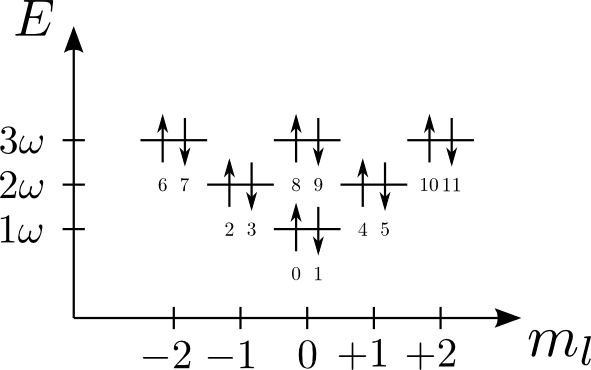
\includegraphics[scale=1.5]{../07-qDots/figs/spektrum.png}
\caption{The indexing sequence used for quantum dots, implemented in `HObasis'.}
\label{fig:qDots:qDotIndex}
\end{center}
\end{figure}


\paragraph{}
All implementations for different systems should extend the `System' base class, which has predefined constructs for holding interaction elements.
The simplest implementation of a system can be as simple as shown in listing~\ref{lst:qDots:SpecificSystem1}, explained as follows;
\begin{itemize}
\item[Line 1:~] We declare a new subclass of `System'. This provides storage objects for both one-particle and two-particle interactions as well as \textit{getter}\footnote{In object-oriented design it is common to encapsulate a class' member objects. Data is then declared private, and can only be reached through public member functions, dubbed getter methods. The author of a class may now restrict how data is accessed, for example to prevent a user from changing important variables.} methods to these storage objects.
\item[Line 4:~] The most important part in the constructor is to create a sensible `Basis', here using the default basis with 2 electrons (hole-states) and 10 virtual (particle-)states. The method `fillMatrixElements()' is defined in `System' and will fill all storage objects with values from `f\_elem' and `v\_elem' using the size of our basis, stored in `basis'.
\item[Line 12:] The normal-ordered one-particle element $f_{pq}$, defined in eq.~\eqref{eq:manybody:f_elem}, is calculated by `f\_elem'. 
\item[Line 21:] The method `v\_elem' defines a way to calculate the antisymmetrized two-particle element $\langle pq || rs \rangle $, defined in eq.~\eqref{eq:manybody:v_elem}.
\end{itemize}
\begin{lstlisting}[float,label={lst:qDots:SpecificSystem1},caption={Example on how to implement a specific system by extending the `System' super class.}]
class SpecificSystem1 : public System
{
public:
	SpecificSystem1()
	{
		std::size_t n_elec = 2;
		std::size_t n_virtual = 10;
		this->basis = new Basis(n_elec, n_virtual);
		fillMatrixElements();
	}
	
	virtual double f_elem(std::size_t p, std::size_t q) const
	{
		double h0_pq = //Some expression for h0
		double u_pq = 0;
		for(size_t i = 0; i < basis->get_nH(); i++)
			u_pq += v_elem(p, i, q, i);
		return h0_pq + u_pq;
	}
	
	virtual double v_elem(std::size_t p, std::size_t q, std::size_t r, std::size_t s) const
	{
		double v_pqrs = //Some expression for <pq||rs>
		return v_pqrs;
	}
};
\end{lstlisting}
One should in particular note that these overridden functions are declared as virtual ones. In this way it is possible to create solvers taking a pointer to any `System', still invoking the methods from the correct subclass. 
Listing~\ref{lst:qDots:virtual_p1} illustrates this, using a `System' pointer to access one single-particle element from a specific subclass.
\begin{lstlisting}[float,label={lst:qDots:virtual_p1},caption={A subclass has implemented the function `f\_elem()' returning the element $f_{02}$. The `System' base class has this method declared virtual, resulting in invoking the subclass implementation even when using a super-class pointer.},name={lst:qDots:virtual}]
//anySystem can point to any system,
System * anySystem = new SpecificSystem();
//and still get an element from the correct subclass
double f_02 = anySystem->f_elem(0,2);
\end{lstlisting}

\paragraph{}
One-particle elements are stored in three matrices: `f\_hh', `f\_ph' and `f\_pp'.
The three matrices are blocks sorted by the domain the two indices $p$ and $q$ belong to.
If both indices are hole states this belongs to `f\_hh' and if both are particle states the element is found in `f\_pp'.
When there is a one-particle state and a one-hole state the `f\_ph' matrix is used, and, since the interaction is Hermitian, we can obtain `f\_hp' as the transposed matrix.

Another way of accessing the same element as in listing~\ref{lst:qDots:virtual_p1} is to use the storage matrices directly. 
The storage matrices for one-particle elements are extracted by calling `get\_f\_hh()', `get\_f\_ph()' or `get\_f\_pp()'.
As an example, we recall `SpecificSystem1' having $n_h = 2$ and $n_p = 10$.
If one would like to extract $f_{02}$ one must note that $2$ is the first particle-state, and $0$ is the first hole-state. 
Indexing starts at zero, and because $f$ is symmetric we see how this can be found in the `f\_ph' part,
\begin{equation}
f_{02} = f_{20} = f^{ph}_{00},
\end{equation}
as implemented in listing~\ref{lst:qDots:virtual_p2}.
\begin{lstlisting}[float,label={lst:qDots:virtual_p2},caption={Continuing listing~\ref{lst:qDots:virtual_p1} extracting the same element, $f_{02}$, now through the raw storage matrix for $f$. This example assumes two occupied (hole) states, thus making index $2$ the first ($0$) particle state. With symmetric interaction matrices we expect $f_{ph} = f_{hp}^T$.},name={lst:qDots:virtual}]
mat const * f_hp;
//Get element from raw storage matrix.
f_hp = trans(anySystem->get_f_ph());
f_02 = (*f_ph)(0,0);
\end{lstlisting}

\paragraph*{}
Although the implementation in listing~\ref{lst:qDots:SpecificSystem1} is very simple, counting only 26 lines of code, this would work perfectly for small systems.
For larger systems one would encounter two problems.
Invoking `fillMatrixElements()' will force calculation of all elements every time a `SpecificSystem1' is constructed, a problem discussed later in section~\ref{sec:qDots:TPfile}.
%MHJ
The other problem is that the dimensionality of the two-particle interactions scales as the number of virtual states to the fourth power. Using symmetries of the interactions one can  reduce the total number of two-body matrix elements. However, for larger numbers of single-particle states, the dimensionalities become large and one 
needs better recipes to handle the increase in dimensionality.


\subsection{Symmetries in the Hamiltonian}
\label{sec:qDots:symHam}
Two-particle matrix elements $\langle pq||rs \rangle$ can be interpreted as the probability for two particles making a transition from states $r$ and $s$ into $p$ and $q$.
If our Hamiltonian preserves some quantum numbers, this transition is not possible, and thus zero, whenever the single-particle states $pq$ do not preserve the numbers from $rs$.
%MHJ 
In the case of quantum dots, we encounter a two-bdoy interaction that is spherically symmetric but not spin dependent.
This results in preserving both the angular-momentum quantum number $m (\equiv m_l)$ as well as spin $m_s$.
Defining $M =m^p + m^q, M' = m^r + m^s$ and $M_s = m_s^p + m_s^q, M'_s = m_s^r + m_s^s$, the following holds true,
\begin{equation}
\langle n^p m^p m_s^p; n^q m^q m_s^q || n^r m^r m_s^r; n^s m^s m_s^s \rangle
= 
0
\hspace{3mm}\textrm{if}\hspace{3mm}
M \neq M'
\hspace{3mm}\textrm{or}\hspace{3mm}
M_s \neq M'_s .
\end{equation}

More generally we define a mapping
$(p,q) \leftrightarrow (\lambda,\pi)$
where $\lambda$ is a transition channel, consisting of a specific set of preserved quantum numbers, and a configuration $\pi$ for each possible combination of $(p,q)$ within that channel, such that 
\begin{equation}
\langle \lambda \pi || \lambda' \pi' \rangle = 0
\hspace{3mm}\textrm{if}\hspace{3mm}
\lambda \neq \lambda' .
\end{equation}
This re-indexing allows us to store the interaction elements as a block-diagonal matrix, one block  for each channel $\lambda$, stored as a matrix $\langle \pi || \pi' \rangle_{\lambda}$.
We further split the interaction matrices whether their indices are above ($a,b,c,d$) or below ($i,j,k,l$) the Fermi-level, resulting in six matrices,
\begin{equation}
\label{eq:qDots:split6tpelem}
\begin{split}
\langle ij||kl \rangle& \\
\langle aj||kl \rangle& = -\langle ja||kl \rangle = \langle kl||aj \rangle = -\langle kl||ja \rangle \\
\langle ab||kl \rangle& = \langle kl||ab \rangle \\
\langle aj||cl \rangle& = -\langle aj||lc \rangle = \langle ja||lc \rangle = -\langle ja||cl \rangle\\
\langle ab||cl \rangle& = -\langle ab||lc \rangle = \langle cl||ab \rangle = \langle lc||ab \rangle \\
\langle ab||cd \rangle&  .\\
\end{split}
\end{equation}
Splitting configurations into configurations for hole-hole states, particle-hole states and particle-particle states, yielding the mappings
\begin{equation}
\begin{split}
(i,j) &\leftrightarrow (\lambda, \mu), \\
(a,j) &\leftrightarrow (\lambda, \nu), \\
(a,b) &\leftrightarrow (\lambda, \xi),
\end{split}
\end{equation}
we can use a storage scheme in `System' objects splitting interactions into six parts similarly to eq.~\eqref{eq:qDots:split6tpelem}, exploiting the sparseness to store block-diagonal parts of the six matrices only, 
\begin{equation}
\begin{split}
\langle \mu || \mu' \rangle_{\lambda},& \hspace{5mm}
\langle \nu || \mu \rangle_{\lambda}, \\
\langle \xi || \mu \rangle_{\lambda},& \hspace{5mm}
\langle \nu || \nu \rangle_{\lambda}, \\ 
\langle \xi || \nu \rangle_{\lambda},& \hspace{5mm}
\langle \xi || \xi \rangle_{\lambda} .
\end{split}
\end{equation}

Mappings from states into channels and configurations are managed by the `Basis' class, and one could access these mappings through the eight methods  in listing~\ref{lst:qDots:accessMappings}.
\begin{lstlisting}[float,label={lst:qDots:accessMappings},caption={There are eight different mappings possible to access through the basis object.}]
//Mappings from (pq,lm,dl,de) into lmd and (pi,mu,nu,xi)
get_map_lmdPI_pq();
get_map_lmdMU_lm();
get_map_lmdNU_dl();
get_map_lmdXI_de();

//Reverse mappings 
get_map_pq_lmdPI();
get_map_lm_lmdMU();
get_map_dl_lmdNU();
get_map_de_lmdXI();
\end{lstlisting}
In this context two general states are encoded to one index, $\mathrm{I}$, i.e.
\begin{equation}
\begin{split}
\mathrm{I}(pq) &= p + q \cdot (n_h + n_p) \\
\mathrm{I}(lm) &= l + m \cdot n_h \\
\mathrm{I}(dl) &= d + l \cdot n_p \\
\mathrm{I}(de) &= d + e \cdot n_p,
\end{split}
\end{equation}
where $n_h$ is the number of hole-states, and $n_p$ the number of particle-states.
Returning to our example of `SpecificSystem1' we have $n_h=2, n_p=10$, and trying to access the matrix element $\langle 20||20 \rangle$ we can use either the procedure from listing~\ref{lst:qDots:mapForward}, extracting the raw matrices, or use the `v\_elem' method as in listing~\ref{lst:qDots:mapBackward}.
\begin{lstlisting}[float,label={lst:qDots:mapForward},caption={We try to access the element $\langle 20||20 \rangle$ by mapping the $|20\rangle$ particle-hole state into a channel and a configuration, $|\nu\rangle_{\lambda}$.},name={lst:qDots:map}]
//Create a specific system
SpecificSystem1 sys;

//Get informations about its basis
Basis const * basis = sys.get_basis();
int nH = basis->get_nH(); //hole-states
int nP = basis->get_nP(); //particle-states

//(d,l) = (2,0) is a particle hole configuration.
int d = 2 - nH;
int l = 0;
int dl = d + l * nH;

//Map into a channel and a configuration.
umat const * map = basis->get_map_dl_lmdNU();
int lmd = (*map)(0,dl); //first row contains lambda values.
int nu = (*map)(1,dl); //second row contains configurations.

//Retrieve element;
vector<mat> const * phph = sys->get_v_phph();
double elem_20_20 = phph->at(lmd)(nu,nu);
\end{lstlisting}
\begin{lstlisting}[float,label={lst:qDots:mapBackward},caption={Continuing listing~\ref{lst:qDots:mapForward}, accessing the same element again, $\langle \nu || \nu \rangle_{\lambda} = \langle 20||20 \rangle$, now using the reverse mapping, $|\nu\rangle_{\lambda} \rightarrow |20\rangle$.},name={lst:qDots:map}]
//Map back to two states d,l
vector<uvec> const * mapback = basis->get_map_lmdNU_dl();
dl = mapback->at(lmd)(nu);
d = dl % nP + nH;
l = dl / nP;

//this should return the same element
elem_20_20 = sys->v_elem(d,l,d,l);
\end{lstlisting}

\paragraph*{}
The default `Basis' base class assumes only one transition channel, resulting in storing all interaction elements.
For quantum dots we have $M,M_s \leftrightarrow \lambda$, implemented in `HOBasis'.
As an example of the reduced dimensionality, we consider a harmonic oscillator basis with 20 electrons and 400 virtual states.
The largest matrix would be $\langle ab||de \rangle$ with a dimensionality of $\sim 400^4$, resulting in $\sim 200$GB of storage!
Exploiting the symmetries and employing an `HOBasis' instead reduces this to $\sim 1.75$GB.
Readers are encouraged to read through this implementation as an example of subclassing `Basis'.



\subsection{Reading elements from file}
\label{sec:qDots:TPfile}
Another time-consuming part is to calculate the matrix elements, which could be performed once and later read from file. 
To create a system read from file, it is convenient to create a subclass of `TPfile', and we take the actual implementation for circular quantum-dots `CQDot' as an example.
There are three methods, shown in listing~\ref{lst:qDots:CQDotMinimumHeader}, which must be overloaded.
\begin{lstlisting}[float,label={lst:qDots:CQDotMinimumHeader},caption={The three most important parts a subclass of `TPfile' would need. The actual implementation of `CQDot' includes some extra methods and private variables.}]
class CQDot : public TPfile
{
public:
  //#1- Constructor
  CQDot(int filledR, int shellsR, double omega = 1.0);
  
  //#2- Calculation of one-particle element f_{pq}
  virtual double f_elem(std::size_t p, std::size_t q) const
  {
    //Part arising from normal ordering
    double u_pq = 0.0;
    for (int i = 0; i < basis->get_nH(); i++)
      u_pq += v_elem(p, i, q, i);
    
	//Part from h0
    ivec3 p_NMMs = basis->stateMap(p);
    int n = pNMMs(0);
    int m = pNMMs(1);
    double h0 = omega * (2 * n + abs(m) + 1);

	//h0 is diagonal
	if (p == q)
      return h0 + u_pq;     
    else
      return u_pq;
  }

protected:
  //#3- A recipe on how to decode tp-element file.
  virtual size_t interp_qNum(char* qNumbers) const;
};
\end{lstlisting}
The constructor takes three arguments; the number of filled shells, the total number of shells and the frequency, $\omega$.

Looking at the constructor's implementation, listing~\ref{lst:qDots:constructor}, we remark how `fillMatrixElements' is no longer called to fill both one- and two-particle elements. 
Instead we read elements $\langle pq||rs \rangle$ from file using `readFileName', and later calculate $f_{pq}$ by invoking 'fillFmatrix'. Both these methods are public, and can therefore be invoked from the main program.
We create a basis, `HOBasis', store the frequency in a private variable, and create a reverse statemap to be used later when reading a file.
This reverse statemap assigns a unique key (unsigned int), constructed from the three quantum numbers, to each state, and it is later possible to get the single index for any state by constructing the same key.
\begin{lstlisting}[float,label={lst:qDots:constructor},caption={Constructor for CQDot.}]
CQDot::CQDot(int filledR, int totalR, double omega)
{
    //Initialize basis and frequency
    basis = new HOBasis(filledR, totalR);
    this->omega = omega;

    //Creating reversed state map, needed when reading file
    int ntot = basis->get_nH() + basis->get_nP();
    for (int state = 0; state < ntot; state++)
    {
    	//Extract quantum numbers n,m,m_s
        ivec3 nmms = basis->stateMap(state);
        unsigned int n = nmms(0);
        int m = nmms(1);
        unsigned int ms = nmms(2);
        
        //Each state has a unique key.
        unsigned int key = n + (m + (ms + hMaxM) * maxM) * maxM;
        revMap[key] = state;
    }
}
\end{lstlisting}

One-particle elements are still calculated through `f\_elem()', implementing the single-particle energies from eq.~\eqref{eq:qDots:spEnergies} combined with a normal-ordered part as in eq.~\eqref{eq:manybody:f_elem}, viz
\begin{equation}
f_{pq} = \delta_{pq} \left(1 + |m| + 2n \right) \omega   + \sum_{i} \langle pi||qi \rangle .
\end{equation}
Depending on $\langle pi||qi \rangle$, one-particle elements are required to be filled after two-particle elements are read from file, by invoking `fillFmatrix'.

Two-particle elements are read through the method `readFileName', redirecting to `readFileStream' in listing~\ref{lst:qDots:readFileStream}.
The file-reading itself is already implemented in the base class, and we expect elements on file to be for $\omega=1$, such that we need only to scale $\omega$ after reading.
Invoking `TPfile::readFileStream' will force the base-class implementation to be run even though these functions are declared as virtual.
The last steps are to scale elements\footnote{Only standard interaction can be scaled by $\sqrt{\omega}$, forcing us to create another file-reading routine `readEffFileStream' (and `readEffFileName') for effective interactions. See section~\ref{ssec:results:veff}.} by $\sqrt{\omega}$ and fill the single-particle elements.
\begin{lstlisting}[float,label={lst:qDots:readFileStream},caption={How to read tp-elements for CQDot.}]
void CQDot::readFileStream(std::ifstream &file)
{
    //First read file as done in super class.
    TPfile::readFileStream(file);
    //Then scale by sqrt(omega)
    size_t dimLMD = basis->dim_lmd_2p();
    for (size_t lmd = 0; lmd < dimLMD; lmd++)
    {
        v_hhhh.at(lmd) = sqrt(omega) * v_hhhh.at(lmd);
        v_phhh.at(lmd) = sqrt(omega) * v_phhh.at(lmd);
        v_pphh.at(lmd) = sqrt(omega) * v_pphh.at(lmd);
        v_phph.at(lmd) = sqrt(omega) * v_phph.at(lmd);
        v_ppph.at(lmd) = sqrt(omega) * v_ppph.at(lmd);
        v_pppp.at(lmd) = sqrt(omega) * v_pppp.at(lmd);
    }
    //Fill one-particle elements.
    fillFmatrix();
}
\end{lstlisting}


\paragraph{}
In order to successfully read elements from file the base class needs some information about the file structure, found through the sub-class implementation of `interp\_qNum'.
A basic file format is expected to be binary with the content,
\begin{verbatim}
p q r s <pq||rs> p' q' r' s' <p'q'||r's'> ... ,
\end{verbatim}
p is a number of bytes, $n_{b}$, needed to specify the state $p$, q is $n_b$ bytes necessary to specify $q$, and so on until the element itself $\langle pq||rs \rangle$ stored as a `double'. 
The implementation for quantum dots may serve as an example.
Here $n,m$ and $m_s$ are coded as an unsigned short, a short and a char. 
This is repeated for all four states an element consists of, followed by the element itself,
\begin{equation}
\underbrace{
\overbrace{n^p}^\text{ushort (2B)} 
\overbrace{m^p}^\text{short (2B)}
\overbrace{m_s^p}^\text{char (1B)}
}_\text{numBytes (5B)}
\underbrace{n^q m^q m_s^q}_\text{(5B)}
\underbrace{n^r\hspace{2mm}m^r\hspace{2mm}m_s^r\hspace{2mm}}_\text{(5B)}
\underbrace{n^s\hspace{2mm}m^s\hspace{2mm}m_s^s\hspace{2mm}}_\text{(5B)}
\underbrace{\langle pq||rs \rangle}_\text{double (8B)} .
\end{equation}
On most platforms this would require 5 bytes for each state, and 8 bytes for the element, as noted in parentheses.
In order to know how many bytes are expected to describe each state, `interp\_qNum(NULL)' is queried.
Once those bytes are read from file they are sent to the same method as a char array, and expected return is a single integer indexing the correct state.
For `CQDot', implementation in listing~\ref{lst:qDots:interp_qNum}, the char array is split into an unsigned short, short and a char, and the correct state is found using the reverse state map that was initialized in the constructor.
\begin{lstlisting}[float,label={lst:qDots:interp_qNum},caption={Implementation of `interp\_qNum' in `CQDot'.}]
size_t CQDot::interp_qNum(char* qNumbers) const
{
    //Quantum numbers n, m, m_s read from file.
    unsigned short n;
    short m;
    char ms;
    
    //Single indexed state
    size_t state;

    //The number of bytes for each state
    if (qNumbers == NULL)
        return sizeof (n) + sizeof (m) + sizeof (ms);

    //Split qNumbers!
    size_t siz_n = sizeof (n);
    memcpy(&n, qNumbers, siz_n);
    size_t siz_m = sizeof (m);
    memcpy(&m, qNumbers + siz_n, siz_m);
    size_t siz_ms = sizeof (ms);
    memcpy(&ms, qNumbers + siz_n + siz_m, siz_ms);

    //Encode spin
    if (ms == -1) 
        ms = 1; //down
    else if (ms == +1)
        ms = 0; //up
    
    //unique key for any state
    unsigned int key = n + (m + (ms + hMaxM) * maxM) * maxM;
    //revMap is a std::map filled in the constructor
    const map<unsigned int, unsigned int>::const_iterator found = revMap.find(key);
    
    if (found == revMap.end())
        state = maxM;  //A state outside the current basis
    else
        state = found->second; //State found in current basis

    return state;
}
\end{lstlisting}


A complete file can be read from file in a simple way, as listing~\ref{lst:qDots:readElem} shows, reading one element at a time, adding a  simple loop to read all elements in a file.
\begin{lstlisting}[float,label={lst:qDots:readElem},caption={How to read two-particle elements from file.}]
void TPfile::readFileStream(std::ifstream &file)
{
  //Number of bytes to read for each state.
  size_t qNumWidth = interp_qNum(NULL);
  char * qNumP = new char[qNumWidth];
  char * qNumQ = new char[qNumWidth];
  char * qNumR = new char[qNumWidth];
  char * qNumS = new char[qNumWidth];

  //Allocate memory for tp-elements.
  //......

  while (true)
  {
    //Read one `line' from file
    double element = 0;
    file.read(qNumP, sizeof (char) * qNumWidth);
    file.read(qNumQ, sizeof (char) * qNumWidth);
    file.read(qNumR, sizeof (char) * qNumWidth);
    file.read(qNumS, sizeof (char) * qNumWidth);
    file.read((char*) &element, sizeof (double));
    if (file.eof())
      break;  //End of file?

	//Find the index
    size_t p = interp_qNum(qNumP);
    size_t q = interp_qNum(qNumQ);
    size_t r = interp_qNum(qNumR);
    size_t s = interp_qNum(qNumS);

    //Store all antisymmetric possibilities 
    storePQRS(p, q, r, s, element);
    storePQRS(p, q, s, r, -element);
    storePQRS(q, p, s, r, element);
    storePQRS(q, p, r, s, -element);
  }

  //Free the four char arrays
  //......
}
\end{lstlisting}
The functionality to read files is already implemented in the `TPfile' class, as the two methods `readFileName' and `readFileStream'.






\section{Other systems}
Other systems may equally well be implemented, and should be compatible with the different solvers as long as they extend the `System' and `Basis' base classes properly.
As an example we have implemented a simple class, `Atoms', outlined in listings~\ref{lst:qDots:atoms_p1} and~\ref{lst:qDots:atoms_p2}, that include the 8 lowest-lying s-states\footnote{Atomic orbitals are distinguished by their angular momentum quantum number $l$. If $l=0$ the state is said to be \textbf{s}harp, an `s-state'. Continuing, for $l=1,2,3$, we have \textbf{p}rinciple, \textbf{d}iffuse and \textbf{f}undamental.} of atomic orbitals.

%MHJ ikke bruk Bohr Model, gi ref til griffith for hydrogen atomet
The single-particle energies are found in the Bohr model to be
\begin{equation}
E_n = \frac{Z^2}{2n^2}, \hspace{4mm}\textrm{(in atomic units)},
\end{equation}
and the two-particle correlation elements are found by integrating the Coloumb energies for the atomic orbitals, either via closed form expressions or computer algebra software, or by numerical integration.
\begin{lstlisting}[float,label={lst:qDots:atoms_p1},caption={Simple implementation for the first sharp atomic orbitals. Continued in listing~\ref{lst:qDots:atoms_p2}.},name={lst:qDots:atoms}]
class Atoms : public System
{
public:
  /** numElec is 2 for helium, 4 for beryllium */
  Atoms(int numElec = 2)
  {
    //Charge from nucleus defaults to number of electrons
    Z = numElec;
    //There are only 8 states implemented
    basis = new Basis(numElec, 8 - numElec);
    //Fill matrices
    fillMatrixElements();
  }

  virtual double f_elem(std::size_t p, std::size_t q) const
  {
    //Normal-ordered part
    double u_pq = 0;
    for (int i = 0; i < basis->get_nH(); i++)
        u_pq += v_elem(p, i, q, i);
	//single-particle energies
    int n = p / 2 + 1;	 //n is the energy level
	double h0 = -pow((double) Z, 2) / (2 * n * n);
	//h0 is diagonal
    if (p == q)
      return h0 + u_pq;
    else
      return u_pq;
  }
\end{lstlisting}
\begin{lstlisting}[float,label={lst:qDots:atoms_p2},caption={Continuation of listing~\ref{lst:qDots:atoms_p1}.},name={lst:qDots:atoms}]
  virtual double v_elem(
    std::size_t p, std::size_t q,
    std::size_t r, std::size_t s) const
  {
    //Get spin of particles
    bool pUP = p % 2 == 0;
	//... same for q,r and s ...

    //Map p,q,r,s to n quantum number
    int n_p = p / 2 + 1;
    //... same for q,r and s ...

    //First term of element
    double term1 = 0;
    if (pUP == rUP && qUP == sUP)
        term1 = spatial_integral(n_p, n_q, n_r, n_s);
    //Second term
    double term2 = 0;
    if (pUP == sUP && qUP == rUP)
        term2 = spatial_integral(n_p, n_q, n_s, n_r);
	
    return term1 - term2;
  }

  /** The spatial integral of correlation energies can be
  /*  found analytically (and tabulated) using Mathematica
  /*  or Maple. Also possible to find through numerical
  /*  integration. (four lowest lying orbitals only) */
  double spatial_integral(int n_p, int n_q, int n_r, int n_s) const;
            
private:
  /** The total charge in the nucleus */
  double Z ;
};
\end{lstlisting}


\paragraph{}
If we were to extend the Harmonic Oscillator basis to three dimension, we would have a basis often used in nuclear physics. 
In that case, one would need one additional quantum numbers for the orbitals, as well as quantum numbers describing different types of particles.
Although not done in this thesis, it should, in the author's opinion, not be too complicated.
However, nuclear calculations often require a larger dimensionality, and further basis considerations (such an angular momentum coupling scheme), see for example
% MHJ Chrsitoffer, legg til ref til Gautes PRC fra 2010.
Hagen {\em et al.} \cite{hagen2010}.





\chapter{Coupled cluster theory}
Coupled cluster~(CC) is an \textit{ab initio} method for solving the quantum mechanical many-body problem.
It was first introduced by Coester and Kümmel during the 1950s \cite{NucPhys.7.421,NucPhys.17.477},
originally developed for problems in nuclear physics, but later reformulated for systems of electrons by \v{C}i\v{z}ek in 1966 \cite{ChemPhys.45.4256}.
Even though it is somewhat computationally expensive it is one of the most popular post-Hartree-Fock methods today, due to good accuracy as well as important features like size-consistency and size-extensivity.

\section{The exponential ansatz}
The foundation for most many-body methods is to express the correct wave function by an expansion in a set of basis functions. 
One example is the Hartree-Fock~(HF) method which employs a unitary transformation of the single-particle wave functions, 
\begin{equation}
|\lambda \rangle = \sum_{\psi} C_{\lambda \psi} |\psi \rangle ,
\end{equation}
and approximates the ground state with a reference Slater determinant built up by these transformed wave functions.
Another example is configuration interaction~(CI) where the reference determinant is set to a linear expansion of determinants, including the initial reference determinant, 1p-1h excitations, 2p-2h excitations and so on, i.e.
\begin{equation}
|\Psi_{0}^{CI} \rangle = C_0 |\Phi_0 \rangle + \sum_{ia} C_i^a |\Phi_i^a\rangle + \sum_{ijab} C_{ij}^{ab} |\Phi_{ij}^{ab} \rangle + \cdots \hspace{2mm}.
\end{equation}
In all these methods one needs to solve a set of coupled equations to find these coefficients.

\paragraph*{}
The Coupled cluster method also expands the exact solution in a set of Slater determinants, but employs a non-linear expansion through the exponential ansatz,
\begin{equation}
\label{eq:CC:expon}
|\Psi_0^{CC} \rangle = e^{\hat{T}} |\Phi_0 \rangle ,
\end{equation}
where $\hat{T}$ is the cluster operator including \textit{all} possible excitations on the reference determinant.
Sorting excitations by the number of excited electrons, we may generally express this general cluster operator as a sum of a 1p-1h operator, a 2p-2h operator, and so on,
\begin{equation}
\hat{T} = \hat{T_1} + \hat{T_2} + \hat{T_3} + \cdots \hspace{2mm}.
\end{equation}
In the form of second-quantized operators the 1p-1h cluster operator is defined as
\begin{equation}
\hat{T}_1 = \sum_{ia} t_i^a \hat{a}^{\dagger} \hat{i},
\end{equation}
the 2p-2h cluster operator as
\begin{equation}
\hat{T}_2 = \frac{1}{4} \sum_{ijab} t_{ij}^{ab} \hat{a}^{\dagger} \hat{b}^{\dagger} \hat{j} \hat{i},
\end{equation}
continuing up to 
\begin{equation}
\hat{T}_n = \left( \frac{1}{n!}\right)^2 \sum_{ij\cdots ab\cdots} t_{ij\cdots}^{ab\cdots} \hat{a}^{\dagger} \hat{b}^{\dagger} \cdots \hat{j} \hat{i} .
\end{equation}
As long as we have a complete single-particle basis and include all possible excitations up to $n$p-$n$h in a system with $n$ particles, we should find the exact solution for both CI, $|\Psi_0^{CI}\rangle$, and CC, $|\Psi_0^{CC}\rangle$.

\paragraph*{}
It is of course not doable to find the exact solution in practice.
A complete single-particle basis would typically mean an infinite set of basis functions.
In addition we would need all excitations up to $n$p-$n$h determinants, yielding a huge amount of determinants. 
This is why all methods need a computational cut-off.
Two types of truncations are used.
First we truncate the number of single-particle basis functions, throwing away the ones with the highest energies, which makes sense since our interest is in the ground-state energy.
Second we truncate the number of excitations we include, giving rise to different types of the coupled cluster method.
Including the singly excited cluster operator the method is labeled by S, for `single', and including the doubly excited cluster operator the label D is added, for `double'.
This thesis has an emphasis on CCSD -- `Coupled Cluster Singles and Doubles'.

\section{Derivation of the CCSD-equations}
It is quite tedious work to derive the CCSD equations by hand, but we will present a diagrammatic approach in this section along with some explaining comments where needed. 

\paragraph{}
We aim to find the solution to the time-independent energy eigenvalue equation,
\begin{equation}
\hat{H} |\Psi_0 \rangle = E_0 |\Psi_0 \rangle
\cong
\hat{H} e^{\hat{T}} |\Phi_0 \rangle = E_0 e^{\hat{T}} |\Phi_0 \rangle ,
\end{equation}
assuming $|\Psi_0\rangle$ can be approximated by the exponential ansatz~\eqref{eq:CC:expon}. 
It is useful to project $\langle \Phi_0 | e^{-\hat{T}}$ onto the eigenvalue equation to get an explicit expression for the energy,
\begin{equation}
\langle \Phi_0 | e^{-\hat{T}} \hat{H} e^{\hat{T}} |\Phi_0 \rangle 
=
\langle \Phi_0 | e^{-\hat{T}} E_0 e^{\hat{T}} |\Phi_0 \rangle
= E_0 .
\end{equation}
We may also project this onto an excited determinant, assuming orthonormal basis functions, and exploit the fact that excited states should be orthogonal to the reference determinant,
\begin{equation}
\langle \Phi_{exc.} | e^{-\hat{T}} \hat{H} e^{\hat{T}} |\Phi_0 \rangle 
=
\langle \Phi_{exc.} | e^{-\hat{T}} E_0 e^{\hat{T}} |\Phi_0 \rangle
=
E_0 \langle \Phi_{exc.} | \hat{1} |\Phi_0 \rangle
= 0 .
\end{equation}
Further simplification is found if we use the normal-ordered Hamiltonian~\eqref{eq:manybody:normhamil}, leading to
\begin{equation}
\begin{split}
\langle \Phi_0 | e^{-\hat{T}} \hat{H}_N e^{\hat{T}} |\Phi_0 \rangle 
=&
\langle \Phi_0 | e^{-\hat{T}} \hat{H} e^{\hat{T}} |\Phi_0 \rangle - E_{ref}
=
E_0 - E_{ref} \\
\langle \Phi_{exc.} | e^{-\hat{T}} \hat{H}_N e^{\hat{T}} |\Phi_0 \rangle 
=&
\langle \Phi_{exc.} | e^{-\hat{T}} (E_0 - E_{ref}) e^{\hat{T}} |\Phi_0 \rangle
=
0 .
\end{split}
\end{equation}


\paragraph*{}
In the following derivation $i,j,k$ and $a,b,c$ will refer to indices in the bra state, whereas 
$d,e,...$ and $l,m,...$ are free indices to be summed over, still restricting $a,b,c,d,e,...$ to particle states and $i,j,k,l,m,...$ to hole states.
There are three equations that, in the case of singles and doubles, needs to be solved,
\begin{equation}
\begin{split}
\langle \Phi_0 | \bar{H} | \Phi_0 \rangle &= E_0  - E_{ref} \\
\langle \Phi_{i}^a | \bar{H} | \Phi_0 \rangle &= 0 \\
\langle \Phi_{ij}^{ab} | \bar{H} | \Phi_0 \rangle &= 0 .
\end{split}
\end{equation}
The first gives us an explicit form for the energy, whereas the other two will determine the amplitudes in the cluster operators.
The similarity transformed Hamiltonian, denoted $\bar{H}$, can be evaluated as a series of commutators, using the Baker-Campbell-Hausdorff formula,
\begin{equation}
\label{eq:CC:BCH}
\bar{H} \equiv e^{-\hat{T}} \hat{H}_N e^{\hat{T}}
=
\hat{H}_N + \left[\hat{H}_N, \hat{T} \right]
+
\frac{1}{2!} \left[\left[\hat{H}_N, \hat{T}\right], \hat{T}\right]
+
\frac{1}{3!} \left[\left[\left[\hat{H}_N, \hat{T} \right], \hat{T}\right], \hat{T}\right] + \cdots\hspace{2mm}.
\end{equation}

Let $\hat{A}$ and $\hat{B}$ be two normal-ordered strings of operators containing an even number of creation and annihilation operators. Using Wick's generalized theorem, their commutator would be
\begin{equation}
\left[ \hat{A}, \hat{B} \right]
=
\left\lbrace \hat{A}\hat{B} \right\rbrace - \left\lbrace \hat{B}\hat{A} \right\rbrace
+
\left\lbrace
\contraction[1ex]{}{\hat{A}}{}{\hat{B}}
\hat{A}\hat{B} \right\rbrace
-
\left\lbrace
\contraction[1ex]{}{\hat{B}}{}{\hat{A}}
\hat{B}\hat{A} \right\rbrace ,
\end{equation}
where the two uncontracted terms are the same, and we thus end up with
\begin{equation}
\left[ \hat{A}, \hat{B} \right]
=
\left\lbrace
\contraction[1ex]{}{\hat{A}}{}{\hat{B}}
\hat{A}\hat{B} \right\rbrace
-
\left\lbrace
\contraction[1ex]{}{\hat{B}}{}{\hat{A}}
\hat{B}\hat{A} \right\rbrace .
\end{equation}
We observe that the cluster operators are already normal-ordered, and also note how no contractions between a cluster operator on the left and any other operator on the right can be non-zero.
This is because the $\hat{T}$ operator contains $\hat{a}^{\dagger} \hat{b}^{\dagger} \cdots \hat{j}\hat{i}$, none of which can lead to any non-zero contraction from~\eqref{eq:manybody:referencecontractions}.
The cluster operators thus commute, yielding
\begin{equation}
\left[ \hat{T}_n, \hat{T}_m \right]
=
\left\lbrace
\contraction[1ex]{}{\hat{T}_n}{}{\hat{T}_m}
\hat{T}_n \hat{T}_m \right\rbrace
-
\left\lbrace
\contraction[1ex]{}{\hat{T}_m}{}{\hat{T}_n}
\hat{T}_m \hat{T}_n \right\rbrace
=
0 .
\end{equation}

We may also explore how the cluster operators commute with the Hamiltonian.
Once again terms with $\hat{T}_n$ on the left are zero, and we are left with
\begin{equation}
\left[ \hat{H}_N, \hat{T}_n \right]
=
\left\lbrace
\contraction[1ex]{}{\hat{H}_N}{}{\hat{T}_n}
\hat{H}_N \hat{T}_n \right\rbrace
-
\left\lbrace
\contraction[1ex]{}{\hat{T}_n}{}{\hat{H}_N}
\hat{T}_n \hat{H}_N \right\rbrace
=
\left\lbrace
\contraction[1ex]{}{\hat{H}}{}{\hat{T}_n}
\hat{H}_N \hat{T}_n \right\rbrace .
\end{equation}
Applying this recursively to write out~\eqref{eq:CC:BCH} it becomes clear that all surviving terms have $\hat{H}_N$ to the left, and all the cluster operators should have at least one contraction each to the Hamiltonian.
These terms are referred to as connected terms (subscript $\mathit{C}$), and because the electronic Hamiltonian includes no more than four operators it would not be possible to find connected terms with more than four cluster operators, posing a natural truncation to $\bar{H}$, 
\begin{equation}
\label{eq:CC:barhconn}
\bar{H} 
= \left(\hat{H}_N e^{\hat{T}} \right)_{\mathit{C}}
= \hat{H}_N 
+ \left( \hat{H}_N \hat{T} \right)_{\mathit{C}}
+\frac{1}{2} \left( \hat{H}_N \hat{T}^2 \right)_{\mathit{C}}
+\frac{1}{3!} \left( \hat{H}_N \hat{T}^3 \right)_{\mathit{C}}
+\frac{1}{4!} \left( \hat{H}_N \hat{T}^4 \right)_{\mathit{C}} .
\end{equation}


\subsection{Diagrammatic rules}
It is now possible to write out all possible terms and evaluate them diagrammatically. 
Writing out each term as a diagram, a number of rules exists on how to interpret them, to find the correct algebraic expressions;
\begin{enumerate}
\item\label{ite:CC:sumFree} Sum over all \textit{free} indices. Free indices are not connected to the left determinant.
\item\label{ite:CC:operators} Interpret one-body operators as $\langle out |\hat{f}| in \rangle \equiv f_{out,in}$, and two-body operators as $\langle lout,rout || lin,rin \rangle$.
\item\label{ite:CC:phase} Add a phase factor of $(-1)^{l+h}$, where $l$ is the number of loops and $h$ is the number of hole lines.
\item\label{ite:CC:equLines} Multiply by a factor of $\frac{1}{2}$ for each pair of \textit{equivalent lines}.
Equivalent lines are starting and ending at the same interaction lines.
\item\label{ite:CC:equVert} Each pair of \textit{equivalent vertices} raises an additional factor of $\frac{1}{2}$.
Equivalent vertices are vertices of equal type connected to the same interaction lines with equivalent connecting lines.
\item\label{ite:CC:permut} Each external, unique pair of holes or particles not connected to the same interaction line leads to an antisymmetric permutation $\hat{P}_{l_1 l_2}$.
\item\label{ite:CC:signTable} If there are multiple ways to connect the diagrams, only one term should exist for each configuration in the Sign-Table technique.
\end{enumerate}
The different rules will be discussed in more detail where needed.

\paragraph*{}
It is possible to split up the sums in the interactions, specifying whether the indices are within the fermi level or not. For the one-body part there exist four possibilities,
\begin{equation}
\hat{F}_N 
=
\sum_{de} f_{de} \left\lbrace \hat{d}^{\dagger} \hat{e} \right\rbrace
+
\sum_{lm} f_{lm} \left\lbrace \hat{l}^{\dagger} \hat{m} \right\rbrace
+
\sum_{ld} f_{ld} \left\lbrace \hat{l}^{\dagger} \hat{d} \right\rbrace
+
\sum_{dl} f_{dl} \left\lbrace \hat{d}^{\dagger} \hat{l} \right\rbrace,
\end{equation}
diagrammatically represented as,
\begin{equation}
\begin{split}
\hat{F}_N
=
\parbox{25mm}{
    \textrm{
    \begin{fmffile}{fmf-cc-F_N-1}
        \begin{fmfgraph*}(50,50)
            %Upper and lower lines.
            \fmfstraight
            \fmfbottom{b1,b2} \fmftop{t1,t2}
            \fmf{phantom}{b1,fL,t1}
            \fmf{phantom}{t2,fR,b2}
            \fmf{dashes}{fL,fR}
            \fmfv{decor.shape=cross,decor.size=3mm}{fR}
            \fmffreeze
            %Electron lines
            \fmf{electron}{b1,fL}
            \fmf{electron}{fL,t1}
        \end{fmfgraph*}
    \end{fmffile}
    }
}
+
\parbox{25mm}{
    \textrm{
    \begin{fmffile}{fmf-cc-F_N-2}
        \begin{fmfgraph*}(50,50)
            %Upper and lower lines.
            \fmfstraight
            \fmfbottom{b1,b2} \fmftop{t1,t2}
            \fmf{phantom}{b1,fL,t1}
            \fmf{phantom}{t2,fR,b2}
            \fmf{dashes}{fL,fR}
            \fmfv{decor.shape=cross,decor.size=3mm}{fR}
            \fmffreeze
            %Electron lines
            \fmf{electron}{t1,fL}
            \fmf{electron}{fL,b1}
        \end{fmfgraph*}
    \end{fmffile}
    }
}
+
\parbox{25mm}{
    \textrm{
    \begin{fmffile}{fmf-cc-F_N-3}
        \begin{fmfgraph*}(50,50)
            %Upper and lower lines.
            \fmfstraight
            \fmfbottom{b1,b2} \fmftop{t1,t2}
            \fmf{phantom}{b1,fL,t1}
            \fmf{phantom}{t2,fR,b2}
            \fmf{phantom}{b1,bC,b2}
            \fmf{dashes}{fL,fR}
            \fmfv{decor.shape=cross,decor.size=3mm}{fR}
            \fmffreeze
            %Electron lines
            \fmf{electron}{b1,fL}
            \fmf{electron}{fL,bC}
        \end{fmfgraph*}
    \end{fmffile}
    }
}
+
\parbox{25mm}{
    \textrm{
    \begin{fmffile}{fmf-cc-F_N-4}
        \begin{fmfgraph*}(50,50)
            %Upper and lower lines.
            \fmfstraight
            \fmfbottom{b1,b2} \fmftop{t1,t2}
            \fmf{phantom}{b1,fL,t1}
            \fmf{phantom}{t2,fR,b2}
            \fmf{phantom}{t1,tC,t2}
            \fmf{dashes}{fL,fR}
            \fmfv{decor.shape=cross,decor.size=3mm}{fR}
            \fmffreeze
            %Electron lines
            \fmf{electron}{t1,fL}
            \fmf{electron}{fL,tC}
        \end{fmfgraph*}
    \end{fmffile}
    }
} .
\end{split}
\end{equation}
The first two terms have the same amount of lines at the top as in the bottom, and we say that these terms have an excitation level zero.
Such terms have no possibility to neither create nor annihilate a particle-hole pair.
If there is an incoming 2p-2h excitation in a diagram, there will also be an outgoing 2p-2h excitation.
The third term is said to have excitation level minus one.
When connected in a diagram it will destroy one particle-hole pair, transforming for example an incoming 2p-2h excitation into an outgoing 1p-1h excitation.
Following this reasoning, the last term has excitation level plus one.

Splitting the two-body operator similarly we get 
\begin{equation}
\begin{split}
\hat{V}_N
=
\parbox{30mm}{
    \textrm{
    \begin{fmffile}{fmf-cc-V_N-1}
        \begin{fmfgraph*}(50,50)
            %Upper and lower lines.
            \fmfstraight
            \fmfbottom{b1,b2,b3,b4} \fmftop{t1,t2,t3,t4}
			\fmf{phantom}{t1,vL,b2}
			\fmf{phantom}{t3,vR,b4}
            \fmffreeze
            \fmf{dashes}{vL,vR}
            %Electron lines
            \fmf{electron}{b1,vL}
            \fmf{electron}{vL,t1}
            \fmf{electron}{b4,vR}
            \fmf{electron}{vR,t4}
        \end{fmfgraph*}
    \end{fmffile}
    }
}
&+
\parbox{30mm}{
    \textrm{
    \begin{fmffile}{fmf-cc-V_N-2}
        \begin{fmfgraph*}(50,50)
            %Upper and lower lines.
            \fmfstraight
            \fmfbottom{b1,b2,b3,b4} \fmftop{t1,t2,t3,t4}
			\fmf{phantom}{t1,vL,b2}
			\fmf{phantom}{t3,vR,b4}
            \fmffreeze
            \fmf{dashes}{vL,vR}
            %Electron lines
            \fmf{electron}{t1,vL}
            \fmf{electron}{vL,b1}
            \fmf{electron}{t4,vR}
            \fmf{electron}{vR,b4}
        \end{fmfgraph*}
    \end{fmffile}
    }
}
+
\parbox{30mm}{
    \textrm{
    \begin{fmffile}{fmf-cc-V_N-3}
        \begin{fmfgraph*}(50,50)
            %Upper and lower lines.
            \fmfstraight
            \fmfbottom{b1,b2,b3,b4} \fmftop{t1,t2,t3,t4}
			\fmf{phantom}{t1,vL,b2}
			\fmf{phantom}{t3,vR,b4}
            \fmffreeze
            \fmf{dashes}{vL,vR}
            %Electron lines
            \fmf{electron}{b1,vL}
            \fmf{electron}{vL,b2}
            \fmf{electron}{t3,vR}
            \fmf{electron}{vR,t4}
        \end{fmfgraph*}
    \end{fmffile}
    }
} \\
&+
\parbox{30mm}{
    \textrm{
    \begin{fmffile}{fmf-cc-V_N-4}
        \begin{fmfgraph*}(50,50)
            %Upper and lower lines.
            \fmfstraight
            \fmfbottom{b1,b2,b3,b4} \fmftop{t1,t2,t3,t4}
			\fmf{phantom}{t1,vL,b2}
			\fmf{phantom}{t3,vR,b4}
            \fmffreeze
            \fmf{dashes}{vL,vR}
            %Electron lines
            \fmf{electron}{b1,vL}
            \fmf{electron}{vL,t1}
            \fmf{electron}{b3,vR}
            \fmf{electron}{vR,b4}
        \end{fmfgraph*}
    \end{fmffile}
    }
}
+
\parbox{30mm}{
    \textrm{
    \begin{fmffile}{fmf-cc-V_N-5}
        \begin{fmfgraph*}(50,50)
            %Upper and lower lines.
            \fmfstraight
            \fmfbottom{b1,b2,b3,b4} \fmftop{t1,t2,t3,t4}
			\fmf{phantom}{t1,vL,b2}
			\fmf{phantom}{t3,vR,b4}
            \fmffreeze
            \fmf{dashes}{vL,vR}
            %Electron lines
            \fmf{electron}{t1,vL}
            \fmf{electron}{vL,b1}
            \fmf{electron}{b3,vR}
            \fmf{electron}{vR,b4}
        \end{fmfgraph*}
    \end{fmffile}
    }
} \\
&+
\parbox{30mm}{
    \textrm{
    \begin{fmffile}{fmf-cc-V_N-6}
        \begin{fmfgraph*}(50,50)
            %Upper and lower lines.
            \fmfstraight
            \fmfbottom{b1,b2,b3,b4} \fmftop{t1,t2,t3,t4}
			\fmf{phantom}{t1,vL,b2}
			\fmf{phantom}{t3,vR,b4}
            \fmffreeze
            \fmf{dashes}{vL,vR}
            %Electron lines
            \fmf{electron}{b1,vL}
            \fmf{electron}{vL,t1}
            \fmf{electron}{t3,vR}
            \fmf{electron}{vR,t4}
        \end{fmfgraph*}
    \end{fmffile}
    }
}
+
\parbox{30mm}{
    \textrm{
    \begin{fmffile}{fmf-cc-V_N-7}
        \begin{fmfgraph*}(50,50)
            %Upper and lower lines.
            \fmfstraight
            \fmfbottom{b1,b2,b3,b4} \fmftop{t1,t2,t3,t4}
			\fmf{phantom}{t1,vL,b2}
			\fmf{phantom}{t3,vR,b4}
            \fmffreeze
            \fmf{dashes}{vL,vR}
            %Electron lines
            \fmf{electron}{t1,vL}
            \fmf{electron}{vL,b1}
            \fmf{electron}{t3,vR}
            \fmf{electron}{vR,t4}
        \end{fmfgraph*}
    \end{fmffile}
    }
} \\
&+
\parbox{30mm}{
    \textrm{
    \begin{fmffile}{fmf-cc-V_N-8}
        \begin{fmfgraph*}(50,50)
            %Upper and lower lines.
            \fmfstraight
            \fmfbottom{b1,b2,b3,b4} \fmftop{t1,t2,t3,t4}
			\fmf{phantom}{t1,vL,b2}
			\fmf{phantom}{t3,vR,b4}
            \fmffreeze
            \fmf{dashes}{vL,vR}
            %Electron lines
            \fmf{electron}{t1,vL}
            \fmf{electron}{vL,t2}
            \fmf{electron}{t3,vR}
            \fmf{electron}{vR,t4}
        \end{fmfgraph*}
    \end{fmffile}
    }
}
+
\parbox{30mm}{
    \textrm{
    \begin{fmffile}{fmf-cc-V_N-9}
        \begin{fmfgraph*}(50,50)
            %Upper and lower lines.
            \fmfstraight
            \fmfbottom{b1,b2,b3,b4} \fmftop{t1,t2,t3,t4}
			\fmf{phantom}{t1,vL,b2}
			\fmf{phantom}{t3,vR,b4}
            \fmffreeze
            \fmf{dashes}{vL,vR}
            %Electron lines
            \fmf{electron}{b1,vL}
            \fmf{electron}{vL,b2}
            \fmf{electron}{b3,vR}
            \fmf{electron}{vR,b4}
        \end{fmfgraph*}
    \end{fmffile}
    }
}.
\end{split}
\end{equation}
The excitation levels are $0$ for the first line, $-1$ for the second, $+1$ for the third, and the last two terms have $+2$ and $-2$ respectively.


Cluster operators are represented with a solid horizontal line for the amplitude as well as electron-lines for the creation and annihilation operators, i.e.
\begin{equation}
\begin{split}
\hat{T}_1
=
\sum_{dl} t_l^d \hat{d}^{\dagger} \hat{l}
=&
\parbox{30mm}{
    \textrm{
    \begin{fmffile}{fmf-cc-T-1}
        \begin{fmfgraph*}(50,50)
            %Upper and lower lines.
            \fmfstraight
            \fmfbottom{b1,b2} \fmftop{t1,t2}
            \fmf{phantom}{b1,tL}
            \fmf{phantom}{tR,b2}
            \fmf{plain}{tL,tC,tR}
            \fmffreeze
            %Electron lines
            \fmf{electron,label=$l$}{t1,tC}
            \fmf{electron,label=$d$}{tC,t2}
        \end{fmfgraph*}
    \end{fmffile}
    }
}  \\
 \\
\hat{T}_2
=
\sum_{delm} t_{lm}^{de} \hat{d}^{\dagger} \hat{e}^{\dagger} \hat{m} \hat{l}
=&
\parbox{40mm}{
    \textrm{
    \begin{fmffile}{fmf-cc-T-2}
        \begin{fmfgraph*}(80,50)
            %Upper and lower lines.
            \fmfstraight
            \fmfbottom{b1,b2} \fmftop{t1,t2,t3,t4}
            \fmf{phantom}{b1,tL}
            \fmf{phantom}{tR,b2}
            \fmf{plain,tension=0.25}{tL,tR}
            \fmffreeze
            %Electron lines
            \fmf{electron,label=$l$}{t1,tL}
            \fmf{electron,label=$d$}{tL,t2}
            \fmf{electron,label=$m$}{t3,tR}
            \fmf{electron,label=$e$}{tR,t4}
        \end{fmfgraph*}
    \end{fmffile}
    }
} .
\end{split} 
\end{equation}
An $n$-body cluster operator creates an $n$p-$n$h excitation, and has thus an excitation level~$+n$.



\subsection{Energy}
The coupled cluster energy $\Delta E_{CCSD} = E_{0} - E_{ref}$ is defined as
\begin{equation}
\langle \Phi_0 | \bar{H} | \Phi_0 \rangle = \Delta E_{CCSD} .
\end{equation}

\subsubsection{$\mathbf{\hat{F}_N}$:}
We will first try to find all terms in eq.~\eqref{eq:CC:barhconn} with cluster operators connected to $\hat{F}_N$.
No lines can be left unconnected, since both the bra and the ket are reference states.
Only the third term in $\hat{F}_N$ can obey this, having no lines pointing upwards and an excitation level of $-1$.
To end up with an excitation level of $0$ we need to connect it with $T_1$ which has a $+1$ excitation level.
Since no electron lines are connected to the bra, they are summed freely over, labelling the particle $d$, and the hole $l$ (rule~\ref{ite:CC:sumFree}).
We have one loop, and one hole line leading to a phase factor $(-1)^{1+1} = +1$ (rule~\ref{ite:CC:phase}).
The interaction has an incoming particle line $d$, and an outgoing hole line $l$, resulting in $f_{out,in} \rightarrow f_{ld}$ (rule~\ref{ite:CC:operators}).
Setting the correct indices for the amplitude as well, this terms yields
\begin{equation}
\hat{F}_N \hat{T}_1 \rightarrow
\parbox{25mm}{
    \textrm{
    \begin{fmffile}{fmf-cc-E-1}
        \begin{fmfgraph*}(50,50)
            %Upper and lower lines.
            \fmfstraight
            \fmfbottom{b1,b2,b3,b4} \fmftop{t1,t2,t3,t4}
            \fmf{plain}{b1,b2,b3}
            \fmf{dashes}{t2,t4}
            %Electron lines
            \fmf{electron,right=0.4}{b2,t2}
            \fmf{electron,right=0.4}{t2,b2}
            %Operator "cross"
            \fmfv{decor.shape=cross,decor.size=3mm}{t4}
        \end{fmfgraph*}
    \end{fmffile}
    }
}
= + \sum_{ld} f_{ld} t_l^d ,
\end{equation}
and is the only contribution from $\hat{F}_N$.


\subsubsection{$\mathbf{\hat{V}_N}$:}
We need to use the last term in $\hat{V}_N$ since all the other terms would leave uncontracted lines pointing upwards, defying the concept of a reference bra state.
Having an excitation level of $-2$ we need to connect it to amplitudes with a $+2$ excitation level.
There are only two possible ways to do this; $\hat{V}_N \hat{T}_2$ and $\hat{V}_N \hat{T}_1^2$.
The first is
\begin{equation}
\hat{V}_N \hat{T}_2
\rightarrow
\parbox{30mm}{
    \textrm{
    \begin{fmffile}{fmf-cc-E-2}
    \begin{fmfgraph*}(50,50)
        %Upper and lover lines
        \fmfstraight
        \fmfbottom{b1,b2}
        \fmftop{t1,t2}
        \fmf{plain}{b1,b2}
        \fmf{dashes}{t1,t2}
        %Electron lines
        \fmf{electron,right=0.4}{b1,t1}
        \fmf{electron,right=0.4}{t1,b1}
        \fmf{electron,right=0.4}{b2,t2}
        \fmf{electron,right=0.4}{t2,b2}
    \end{fmfgraph*}
    \end{fmffile}
    }
}
= + \frac{1}{4} \sum_{lmde} \langle lm|| de \rangle t_{lm}^{de}, 
\end{equation}
a term with two hole lines as well as two loops and thus a positive phase.
All indices are freely summed, but since both the pair of particle lines and the pair of hole lines starts and stops and the same interaction, they are equivalent, and should be multiplied by $\left(\frac{1}{2}\right)^2 = \frac{1}{4}$ (rule~\ref{ite:CC:equLines}).

The last term in the energy has also two hole lines and two loops, but since there are two $\hat{T}_1$ operators, the particle and hole lines are no longer equivalent.
These are two equivalent vertices instead, raising a factor $\frac{1}{2}$ (rule~\ref{ite:CC:equVert}) and resulting in 
\begin{equation}
\hat{V}_N \hat{T}_1^2
\rightarrow
\parbox{28mm}{
    \textrm{
    \begin{fmffile}{fmf-cc-E-3}
        \begin{fmfgraph*}(50,50)
            %references
            \fmfstraight
            \fmfbottom{b1,b2,b3,b4}
            \fmftop{t1,t2}
            %bottom t1 lines
            \fmf{plain}{b1,elBotL,b2}
            \fmf{plain}{b3,elBotR,b4}
            %top lines
            \fmf{phantom,tension=4}{t1,elTopL}
            \fmf{phantom,tension=4}{elTopR,t2}
            \fmf{dashes}{elTopL,elTopR}
            \fmffreeze
            %electron lines
            \fmf{electron,right=0.4}{elBotL,elTopL}
            \fmf{electron,right=0.4}{elTopL,elBotL}
            \fmf{electron,right=0.4}{elBotR,elTopR}
            \fmf{electron,right=0.4}{elTopR,elBotR}
        \end{fmfgraph*}
    \end{fmffile}
    }
}
= +\frac{1}{2} \sum_{lmde} \langle lm||de \rangle t_l^d t_m^e .
\end{equation}

Adding these terms together we end up with the complete energy equation
\begin{equation}
\Delta E_{CCSD} = 
\sum_{ld} f_{ld} t_l^d
+ \frac{1}{4} \sum_{lmde} \langle lm|| de \rangle t_{lm}^{de}
+\frac{1}{2} \sum_{lmde} \langle lm||de \rangle t_l^d t_m^e,
\end{equation}
giving us the correction to the energy as compared to $E_{ref}$ for a given set of amplitudes $t_{i}^{a}$ and $t_{ij}^{ab}$.


\subsection{T1 equations}
We will need the amplitude equations to find these amplitudes, starting with the $\hat{T}_1$ equations derived from
\begin{equation}
\langle \Phi_i^a | \bar{H} | \Phi_0 \rangle = 0 .
\end{equation}
Because of the singly excited bra determinant we will need a total excitation level of $+1$.
Terms are presented in the same order as in equation~\eqref{eq:CC:barhconn}.

\subsubsection{$\mathbf{\hat{H}_N}$:}
With a reference ket at the bottom and expecting a singly excited determinant bra at the top, we need a term with excitation level $+1$ and no electron lines pointing downwards. 
There is only one appropriate term for this,
\begin{equation}
\langle \Phi_i^a | \hat{F}_N | \Phi_0 \rangle 
\rightarrow 
\parbox{30mm}{
    \textrm{
    \begin{fmffile}{fmf-cc-t1-1}
        \begin{fmfgraph*}(50,50)
            \fmfstraight
            \fmfbottom{b1,b2,b3,b4}
            \fmftop{t1,t2,t3,t4}
            %F operator
            \fmf{dashes}{b2,b4}
            \fmfv{decor.shape=cross,decor.size=3mm}{b4}
            %electrons
            \fmf{electron}{t1,b2}
            \fmf{electron}{b2,t3}
        \end{fmfgraph*}
    \end{fmffile}
    }
}
= + f_{ai} .
\end{equation}
Both electron lines are connected to the singly excited bra state, labeled $i,a$, and thus not summed freely over.
With one hole line and one loop (particle-hole excitations are `connected' in the bra determinant) the factor in front is $+1$.

\subsubsection{$\mathbf{\hat{H}_N \hat{T}}$:}
Connecting terms from $\hat{H}_N$ first with the $\hat{T}_1$ cluster operators the total excitation level needs to be $+1$, already supplied by the singly excited cluster operator.
We then require interaction terms that neither create nor destroy particle-hole excitations.
Three possible interaction terms fit in; two from $\hat{F}_N$,
\begin{equation}
\langle \Phi_i^a | \hat{F}_N \hat{T}_1 | \Phi_0 \rangle 
\rightarrow
\parbox{30mm}{
    \textrm{
    \begin{fmffile}{fmf-cc-t1-2}
        \begin{fmfgraph*}(50,50)
            \fmfstraight
            \fmfbottom{b1,b2,b3,b4}
            \fmftop{t1,t2,t3,t4}
            %T_1 operator
            \fmf{plain}{b1,b2,b3}
            %F operator
            \fmf{phantom}{t4,fR,b4}
            \fmf{dashes,tension=0}{fL,fR}
            \fmfv{decor.shape=cross,decor.size=3mm}{fR}
            %electrons
            \fmf{electron}{t1,b2}
            \fmf{electron}{b2,fL}
            \fmf{electron}{fL,t3}
        \end{fmfgraph*}
    \end{fmffile}
    }
}
+
\parbox{30mm}{
    \textrm{
    \begin{fmffile}{fmf-cc-t1-3}
        \begin{fmfgraph*}(50,50)
            \fmfstraight
            \fmfbottom{b1,b2,b3,b4}
            \fmftop{t1,t2,t3,t4}
            %T_1 operator
            \fmf{plain}{b2,b3,b4}
            %F operator
            \fmf{phantom}{t1,fL,b1}
            \fmf{dashes,tension=0}{fL,fR}
            \fmfv{decor.shape=cross,decor.size=3mm}{fL}
            %electrons
            \fmf{electron}{t2,fR}
            \fmf{electron}{fR,b3}
            \fmf{electron}{b3,t4}
        \end{fmfgraph*}
    \end{fmffile}
    }
}
= + \sum_d f_{ad} t_i^d - \sum_l f_{li} t_l^a ,
\end{equation}
and one from $\hat{V}_N$,
\begin{equation}
\langle \Phi_i^a | \hat{V}_N \hat{T}_1 | \Phi_0 \rangle 
\rightarrow
\parbox{30mm}{
    \textrm{
    \begin{fmffile}{fmf-cc-t1-4}
        \begin{fmfgraph*}(50,50)
        \fmfstraight
        \fmfbottom{b1,b2,b3,b4,b5}
        \fmftop{t1,t2,t3,t4,t5}
        %prepare fixed middle points
        \fmf{phantom}{b1,mL,t1}
        \fmf{phantom}{b5,mR,t5}
        \fmffreeze
        %T_1 operator
        \fmf{plain}{b1,b2,b3}
        %V_N operator
        \fmf{phantom,tension=2}{mL,vL}
        \fmf{phantom,tension=2}{mR,vR}
        \fmf{dashes}{vL,vR}
        \fmffreeze
        %Electrons
        \fmf{electron}{t3,vR}
        \fmf{electron}{vR,t5}
        \fmf{electron,right=0.4}{b2,vL}
        \fmf{electron,right=0.4}{vL,b2}
        \end{fmfgraph*}
    \end{fmffile}
    }
}
= + \sum_{ld} \langle la||di \rangle t_l^d .
\end{equation}
There are also three terms where the interactions are connected to $\hat{T}_2$, requiring the interactions to have the ability to annihilate one particle-hole excitation.
One term connects to $\hat{F}_N$,
\begin{equation}
\label{eq:CC:FnT2}
\langle \Phi_i^a | \hat{F}_N \hat{T}_2 | \Phi_0 \rangle 
\rightarrow
\parbox{30mm}{
    \textrm{
    \begin{fmffile}{fmf-cc-t1-5}
        \begin{fmfgraph*}(50,50)
            \fmfstraight
            \fmfbottom{b1,b2}
            \fmftop{t1,t2,t3}
            %T_2 operator
            \fmf{phantom,tension=2}{b1,tL}
            \fmf{phantom,tension=2}{tR,b2}
            \fmf{plain}{tL,tR}
            \fmffreeze
            %V_N Operator
            \fmf{phantom}{b2,vL,t2}
            \fmf{phantom}{b2,vR,t3}
            \fmf{dashes,tension=0}{vL,vR}
            \fmfv{decor.shape=cross,decor.size=3mm}{vR}
            \fmffreeze
            %electrons
            \fmf{electron}{t1,tL}
            \fmf{electron}{tL,t2}
            \fmf{electron,right=0.4}{tR,vL}
            \fmf{electron,right=0.4}{vL,tR}
        \end{fmfgraph*}
    \end{fmffile}
    }
}
= + \sum_{ld} f_{ld} t_{il}^{ad},
\end{equation}
and the other two to $\hat{V}_N$,
\begin{equation}
\label{eq:CC:VnT2}
\begin{split}
\langle \Phi_i^a | \hat{V}_N \hat{T}_2 | \Phi_0 \rangle 
\rightarrow &
\parbox{30mm}{
    \textrm{
    \begin{fmffile}{fmf-cc-t1-6}
        \begin{fmfgraph*}(50,50)
            \fmfstraight
            \fmfbottom{b1,b2}
            \fmftop{t1,t2,t3}
            %T_2 operator
            \fmf{phantom,tension=2}{b1,tL}
            \fmf{plain}{tL,b2}
            \fmffreeze
            %electrons
            \fmf{electron}{t1,tL}
            \fmf{electron}{tL,vL,t2}
            \fmf{electron,right=0.4}{b2,vR}
            \fmf{electron,right=0.4}{vR,b2}
            \fmf{phantom,tension=2}{vR,t3}
            %V_N operator
            \fmf{dashes,tension=0}{vR,vL}
        \end{fmfgraph*}
    \end{fmffile}
    }
}
+
\parbox{30mm}{
    \textrm{
    \begin{fmffile}{fmf-cc-t1-7}
        \begin{fmfgraph*}(50,50)
            \fmfstraight
            \fmfbottom{b1,b2}
            \fmftop{t1,t2,t3}
            %T_2 operator
            \fmf{phantom,tension=2}{b2,tR}
            \fmf{plain}{tR,b1}
            \fmffreeze
            %electrons
            \fmf{electron}{t2,vR,tR}
            \fmf{electron}{tR,t3}
            \fmf{electron,right=0.4}{b1,vL}
            \fmf{electron,right=0.4}{vL,b1}
            \fmf{phantom,tension=2}{vL,t1}
            %V_N operator
            \fmf{dashes,tension=0}{vR,vL}
        \end{fmfgraph*}
    \end{fmffile}
    }
} \\
 \\
= & + \frac{1}{2} \sum_{lde} \langle al||de \rangle t_{il}^{de} - \frac{1}{2} \sum_{lmd}
\langle lm||di \rangle t_{lm}^{da} .
\end{split} 
\end{equation}

\subsubsection{$\mathbf{\hat{H}_N \hat{T}^2}$:}
The cluster operator to second order has three terms\footnote{Factors in front of terms are found using the diagrammatic rules, allowing us to neglect the factor of two in the cross term.},
\begin{equation}
\hat{H}_N \left( \hat{T}_1 + \hat{T}_2 \right)^2
\rightarrow
\hat{H}_N \hat{T}_1^2 + \hat{H}_N \hat{T}_1 \hat{T}_2 + \hat{H}_N \hat{T}_2^2,
\end{equation}
and we may first note how no contraction between $\hat{T}_2^2$ and any interaction term can be made without resulting in at least a doubly excited bra state.
This leaves us with $\hat{T}_1^2$ and the cross term $\hat{T}_1\hat{T}_2$.
For $\hat{T}_1^2$ we can connect the same interaction terms as for $\hat{T}_2$ in eq.~\eqref{eq:CC:FnT2} and~\eqref{eq:CC:VnT2},
\begin{equation}
\langle \Phi_i^a | \hat{F}_N \hat{T}_1^2 | \Phi_0 \rangle 
\rightarrow
\parbox{30mm}{
    \textrm{
    \begin{fmffile}{fmf-cc-t1-8}
        \begin{fmfgraph*}(50,50)
            \fmfstraight
            \fmftop{t1,t2}
            \fmfbottom{b1,b2,b3,b4}
            %T_1 operators
            \fmf{plain}{b1,tL,b2}
            \fmf{plain}{b3,tR,b4}
            \fmffreeze
            %Electrons 
            \fmf{electron}{t1,tL}
            \fmf{electron}{tL,fL}
            \fmf{electron}{fL,tR}
            \fmf{electron}{tR,t2}
            %F operator
            \fmf{phantom,tension=2}{t1,fL}
            \fmf{phantom,tension=2}{t2,fR}
            \fmf{phantom}{tL,fR,tR}
            \fmf{dashes}{fL,fR}
            \fmfv{decor.shape=cross,decor.size=3mm}{fR}
        \end{fmfgraph*}
    \end{fmffile}
    }
}
= - \sum_{ld} f_{ld} t_i^d t_l^a ,
\end{equation}
and 
\begin{equation}
\begin{split}
\langle \Phi_i^a | \hat{V}_N \hat{T}_1^2 | \Phi_0 \rangle \rightarrow &
\parbox{30mm}{
    \textrm{
    \begin{fmffile}{fmf-cc-t1-9}
        \begin{fmfgraph*}(50,50)
            \fmfstraight
            \fmftop{t1,t2,t3,t4}
            \fmfbottom{b1,b2,b3,b4}
            %T_1 operators
            \fmf{plain}{b1,tL,b2}
            \fmf{plain}{b3,tR,b4}
            \fmf{phantom}{t3,phant,t4}
            \fmffreeze
            %Electron lines
            \fmf{electron}{t1,tL}
            \fmf{electron}{tL,vL}
            \fmf{electron}{vL,t3}
            \fmf{electron,right=0.4}{tR,vR}
            \fmf{electron,right=0.4}{vR,tR}
            \fmf{phantom,tension=2}{phant,vR}
            %V_N operator
            \fmf{dashes,tension=0}{vL,vR}
        \end{fmfgraph*}
    \end{fmffile}
    }
}
+
\parbox{30mm}{
    \textrm{
    \begin{fmffile}{fmf-cc-t1-10}
        \begin{fmfgraph*}(50,50)
            \fmfstraight
            \fmftop{t1,t2,t3,t4}
            \fmfbottom{b1,b2,b3,b4}
            %T_1 operators
            \fmf{plain}{b1,tL,b2}
            \fmf{plain}{b3,tR,b4}
            \fmf{phantom}{t1,phant,t2}
            \fmffreeze
            %Electron lines
            \fmf{electron}{t2,vR}
            \fmf{electron}{vR,tR}
            \fmf{electron}{tR,t4}
            \fmf{electron,right=0.4}{tL,vL}
            \fmf{electron,right=0.4}{vL,tL}
            \fmf{phantom,tension=2}{phant,vL}
            %V_N operator
            \fmf{dashes,tension=0}{vL,vR}
        \end{fmfgraph*}
    \end{fmffile}
    }
} \\
 \\
= & + \sum_{lde} \langle al||de \rangle t_i^d t_l^e 
- \sum_{lmd} \langle lm||di \rangle t_l^d t_m^a .
\end{split}
\end{equation}
For the cross term, $\hat{T}_1 \hat{T}_2$, we need an operator with excitation level $-2$. Only the last $\hat{V}_N$ term has this level, but it can be connected in three distinct ways,
\begin{equation}
\label{eq:CC:T1crossT}
\begin{split}
\langle \Phi_i^a | \hat{V}_N \hat{T}_1 \hat{T}_2 | \Phi_0 \rangle \rightarrow &
\parbox{33mm}{
    \textrm{
    \begin{fmffile}{fmf-cc-t1-11}
        \begin{fmfgraph*}(80,50)
            \fmfstraight
            \fmftop{t1,t2}
            \fmfbottom{b1,b2,b3,b4,b5}
            %T_1 and T_2
            \fmf{plain}{b1,tL,b2}
            \fmf{plain}{b3,tR}
            \fmf{phantom,tension=3}{tR,b5}
            \fmffreeze
            %V_N operator
            \fmf{dashes}{vL,vR}
            %Electrons
            \fmf{electron}{t1,tL}
            \fmf{electron}{tL,vL}
            \fmf{electron}{vL,b3}
            \fmf{electron}{b3,vR}
            \fmf{electron}{vR,tR}
            \fmf{electron}{tR,t2}
            %"Lift" operator line a bit
            \fmf{phantom,tension=2.0}{t1,vL}
            \fmf{phantom,tension=2.0}{vR,t2}
        \end{fmfgraph*}
    \end{fmffile}
    }
}
+
\parbox{33mm}{
    \textrm{
    \begin{fmffile}{fmf-cc-t1-12}
        \begin{fmfgraph*}(80,50)
            \fmfstraight
            \fmftop{t1,t2}
            \fmfbottom{b1,b2,b3,b4,b5}
            %T_1 and T_2
            \fmf{plain}{b4,tR,b5}
            \fmf{plain}{tL,b3}
            \fmf{phantom,tension=3}{b1,tL}
            \fmffreeze
            %V_N operator
            \fmf{dashes}{vL,vR}
            %Electrons
            \fmf{electron}{t1,tL}
            \fmf{electron}{tL,vL}
            \fmf{electron}{vL,b3}
            \fmf{electron}{b3,vR}
            \fmf{electron}{vR,tR}
            \fmf{electron}{tR,t2}
            %"Lift" operator line a bit
            \fmf{phantom,tension=2.0}{t1,vL}
            \fmf{phantom,tension=2.0}{vR,t2}
        \end{fmfgraph*}
    \end{fmffile}
    }
}
+
\parbox{33mm}{
    \textrm{
    \begin{fmffile}{fmf-cc-t1-13}
        \begin{fmfgraph*}(80,50)
            \fmfstraight
            \fmftop{t1,t2,t3,t4,t5}
            \fmfbottom{b1,b2,b3,b4,b5}
            %T_1 and T_2
            \fmf{plain}{b4,tR,b5}
            \fmf{plain}{tL,b3}
            \fmf{phantom,tension=3}{b1,tL}
            \fmffreeze
            %Electrons
            \fmf{electron}{t1,tL}
            \fmf{electron}{tL,t2}
            \fmf{electron,right=0.4}{vL,b3}
            \fmf{electron,right=0.4}{b3,vL}
            \fmf{electron,right=0.4,tension=0}{vR,tR}
            \fmf{electron,right=0.4,tension=0}{tR,vR}
            %V_N operator
            \fmf{phantom,tension=2}{t3,vL}
            \fmf{phantom}{b4,vR,t5}
            \fmffreeze
            \fmf{dashes}{vL,vR}
        \end{fmfgraph*}
    \end{fmffile}
    }
} \\
 \\
= &
 \frac{1}{2} \sum_{lmde} \langle lm||de \rangle t_i^d t_{lm}^{ea} 
+ \frac{1}{2} \sum_{lmde} \langle lm||de \rangle t_m^a t_{il}^{de}
+ \sum_{lmde} \langle lm||de \rangle t_m^e t_{il}^{ad}.
\end{split}
\end{equation}
In order to find all unique ways of connecting the operators together, the sign-table technique is applied (rule~\ref{ite:CC:signTable}).
Denoting a plus sign for all particle lines in the interaction that are connectable to amplitudes (below the interaction line), and a minus sign for all connectable hole lines, we set up a table for what lines are connected to which amplitude.
The term from $\hat{V}_N$ used in eq.~\eqref{eq:CC:T1crossT} has two particle and two hole lines below the interaction line, represented by a string of four signs, $++--$.
A sign table consists of one column for each of the cluster operators, and distinct terms exist for each unique way the signs are distributed.
\begin{table}
\caption{Sign table for the three terms in eq.~\eqref{eq:CC:T1crossT}.}
\label{tab:CC:SignT1crossT}
\begin{center}
\begin{tabular}{c|c}
$\hat{T}_1$ & $\hat{T}_2$ \\ 
\hline 
$+$ & $+--$ \\ 
$-$ & $++-$ \\ 
$+-$ & $+-$ 
\end{tabular} 
\end{center}
\end{table}
The three distinct terms from equation~\eqref{eq:CC:T1crossT} are represented in table~\ref{tab:CC:SignT1crossT} in the same order as the terms appear in the equation.
Adding more than one $+$ or more than one $-$ to $\hat{T}_1$ would be impossible here, due to its one-particle one-hole nature, and leaving $\hat{T}_1$ empty would lead to an uncontracted term.
For this reason we get only the three terms seen.

\subsubsection{$\mathbf{\hat{H}_N \hat{T}^3}$:}
No term in the normal-ordered Hamiltonian can annihilate more than a 2p-2h excitation, and since the bra determinant is singly excited, at most a triple excitation can arise from the cluster operators.
The last possible term is thus connected to $\hat{T}_1^3$, 
\begin{equation}
\langle \Phi_i^a | \hat{V}_N \hat{T}_1^3 | \Phi_0 \rangle \rightarrow 
\parbox{36mm}{
    \textrm{
    \begin{fmffile}{fmf-cc-t1-14}
        \begin{fmfgraph*}(80,50)
            \fmfstraight
            \fmftop{t1,t2}
            \fmfbottom{b1,b2,b3,b4,b5,b6}
            %T_1 operators (left,middle,right)
            \fmf{plain}{b1,tL,b2}
            \fmf{plain}{b3,tM,b4}
            \fmf{plain}{b5,tR,b6}
            \fmffreeze
            %Electrons
            \fmf{electron}{t1,tL}
            \fmf{electron}{tL,vL}
            \fmf{electron}{vL,tM}
            \fmf{electron}{tM,vR}
            \fmf{electron}{vR,tR}
            \fmf{electron}{tR,t2}
            %V_N operator
            \fmf{dashes}{vL,vR}
            \fmf{phantom,tension=2}{t1,vL}
            \fmf{phantom,tension=2}{vR,t2}
        \end{fmfgraph*}
    \end{fmffile}
    }
}
=
+ \sum_{lmde} \langle lm||de \rangle t_i^d t_l^e t_m^a .
\end{equation}


\paragraph*{}
Adding all terms together we get the complete $\hat{T}_1$ amplitude equations;
\begin{equation}
\label{eq:CC:t1eq_raw}
\begin{split}
0 =& f_{ai}
+ \sum_d f_{ad} t_i^d - \sum_l f_{li} t_l^a
 + \sum_{ld} \langle la||di \rangle t_l^d
\\
 &+ \sum_{ld} f_{ld} t_{il}^{ad}
 + \frac{1}{2} \sum_{lde} \langle al||de \rangle t_{il}^{de} - \frac{1}{2} \sum_{lmd}
\langle lm||di \rangle t_{lm}^{da}  
- \sum_{ld} f_{ld} t_i^d t_l^a
\\
& + \sum_{lde} \langle al||de \rangle t_i^d t_l^e 
- \sum_{lmd} \langle lm||di \rangle t_l^d t_m^a
+ \frac{1}{2} \sum_{lmde} \langle lm||de \rangle t_i^d t_{lm}^{ea} 
\\
&+ \frac{1}{2} \sum_{lmde} \langle lm||de \rangle t_m^a t_{il}^{de}
+ \sum_{lmde} \langle lm||de \rangle t_m^e t_{il}^{ad}
+ \sum_{lmde} \langle lm||de \rangle t_i^d t_l^e t_m^a .
\end{split}
\end{equation}


\subsection{T2 equations}
We continue by finding algebraic expressions for the $\hat{T}_2$ equations, 
\begin{equation}
\langle \Phi_{ij}^{ab} | \bar{H} | \Phi_0 \rangle = 0 ,
\end{equation}
utilizing the same techniques as before, also introducing permutatation of external lines in eq~\eqref{eq:CC:t2permutation}.
Terms are once again sorted in the same order as in $\bar{H}$ $\eqref{eq:CC:barhconn}$, now requiring a doubly excited particle-hole pair to accommodate the bra determinant.


\subsubsection{$\mathbf{\hat{H}_N}$:}
The only interaction term to have a double particle-hole excitation comes from $\hat{V}_N$, 
\begin{equation}
\langle \Phi_{ij}^{ab} | \hat{V}_N | \Phi_0 \rangle \rightarrow
\parbox{25mm}{
    \textrm{
    \begin{fmffile}{fmf-cc-t2-1}
        \begin{fmfgraph*}(50,50)
            \fmfstraight
            \fmftop{u1,u2,u3,u4}
            \fmfbottom{b1,b2}
            %V_N operator
            \fmf{dashes}{vL,vR}
            \fmf{phantom,tension=4}{b1,vL}
            \fmf{phantom,tension=4}{vR,b2}
            \fmffreeze
            %Electrons
            \fmf{electron}{u1,vL}
            \fmf{electron}{vL,u2}
            \fmf{electron}{u3,vR}
            \fmf{electron}{vR,u4}
        \end{fmfgraph*}
    \end{fmffile}
    }
}
= \langle ab || ij \rangle .
\end{equation}


\subsubsection{$\mathbf{\hat{H}_N \hat{T}}$:}
A consequence of having more than one pair of external particle and hole lines from the bra determinant is that two different particle-, or hole-lines may be connected to different operators.
In the following two terms we have labeled the external lines from left to right, $i,a,j,b$,
\begin{equation}
\label{eq:CC:t2permutation}
\begin{split}
\langle \Phi_{ij}^{ab} | \hat{V}_N \hat{T}_1 | \Phi_0 \rangle \rightarrow& 
\parbox{27mm}{
    \textrm{
    \begin{fmffile}{fmf-cc-t2-2}
        \begin{fmfgraph*}(50,50)
            \fmfstraight
            \fmftop{u1,u2,u3,u4}
            \fmfbottom{b1,b2,b3,b4}
            %T_1 operator
            \fmf{plain}{b1,t1,b2}
            \fmffreeze
            %Electron lines
            \fmf{electron}{u1,t1}
            \fmf{electron}{t1,vL}
            \fmf{electron}{vL,u2}
            \fmf{electron}{u3,vR}
            \fmf{electron}{vR,u4}
            %Lower the two rightmost to the middle
            \fmf{phantom}{b3,vR,b4}
            \fmffreeze
            %V_N operator
            \fmf{dashes}{vL,vR}
        \end{fmfgraph*}
    \end{fmffile}
    }
}
+
\parbox{27mm}{
    \textrm{
    \begin{fmffile}{fmf-cc-t2-3}
        \begin{fmfgraph*}(50,50)
            \fmfstraight
            \fmftop{u1,u2,u3,u4}
            \fmfbottom{b1,b2,b3,b4}
            %T_1 operator
            \fmf{plain}{b3,t1,b4}
            \fmffreeze
            %Electrons
            \fmf{electron}{u1,vL}
            \fmf{electron}{vL,u2}
            \fmf{electron}{u3,vR}
            \fmf{electron}{vR,t1}
            \fmf{electron}{t1,u4}
            %Lower the leftmost p/h pair
            \fmf{phantom}{b1,vL,b2}
            \fmffreeze
            %V_N operator
            \fmf{dashes}{vL,vR}
        \end{fmfgraph*}
    \end{fmffile}
    }
} \\
 \\
=&
\hat{P}_{ij} \sum_{d} \langle ab || dj \rangle t_i^d
-
\hat{P}_{ab} \sum_l \langle al||ij \rangle t_l^b .
\end{split}
\end{equation}
The first term has $i$ connected to $\hat{T}_1$, whereas $j$ is connected to $\hat{V}_N$, and the second term has $a$ connected to $\hat{V}_N$, whereas $b$ is connected to $\hat{T}_1$.
Whenever two such lines are connected to the same interaction a permutation is implied through the antisymmetric nature of the elements, i.e.
\begin{equation}
\langle pq || rs \rangle = - \langle pq||sr \rangle = \cdots
\hspace{3mm}\textrm{or}\hspace{3mm}
t_{ij}^{ab} = -t_{ji}^{ab} = \cdots\hspace{2mm}.
\end{equation}
In the cases where such a permutation is not implied, we need to enforce a permutation, as in equation~\eqref{eq:CC:t2permutation}.

No permutations arose in the $\hat{T}_1$ equations due to the fact that only one particle and one hole line were connected upwards to the singly excited determinant.
Now, in the $\hat{T}_2$ equations, we have a doubly excited determinant, with the consequence of more terms requiring permutations, as seen also in the terms from $\hat{H}_N \hat{T}_2$;
\begin{equation}
\begin{split}
\langle \Phi_{ij}^{ab} | \hat{F}_N \hat{T}_2 | \Phi_0 \rangle \rightarrow& 
\parbox{30mm}{
    \textrm{
    \begin{fmffile}{fmf-cc-t2-4}
        \begin{fmfgraph*}(60,50)
            \fmfstraight
            \fmftop{u1,u2,u3,u4,u5}
            \fmfbottom{b1,b2,b3,b4,b5}
            %T_2 operator
            \fmf{phantom}{b1,t2L}
            \fmf{plain,tension=0.25}{t2L,t2R}
            \fmf{phantom}{t2R,b4}
            \fmffreeze
            %Electrons
            \fmf{electron}{u1,t2L}
            \fmf{electron}{t2L,u2}
            \fmf{electron}{u3,t2R}
            \fmf{electron}{t2R,fL}
            \fmf{electron}{fL,u4}
            %F_N operator
            \fmf{phantom}{u5,fR,b5}
            \fmffreeze
            \fmf{dashes}{fL,fR}
            \fmfv{decor.shape=cross,decor.size=3mm}{fR}
        \end{fmfgraph*}
    \end{fmffile}
    }
}
+
\parbox{30mm}{
    \textrm{
    \begin{fmffile}{fmf-cc-t2-5}
        \begin{fmfgraph*}(60,50)
            \fmfstraight
            \fmftop{u1,u2,u3,u4,u5}
            \fmfbottom{b1,b2,b3,b4,b5}
            %T_2 operator
            \fmf{phantom}{b2,t2L}
            \fmf{plain,tension=0.25}{t2L,t2R}
            \fmf{phantom}{t2R,b5}
            \fmffreeze
            %Electrons
            \fmf{electron}{u2,fR}
            \fmf{electron}{fR,t2L}
            \fmf{electron}{t2L,u3}
            \fmf{electron}{u4,t2R}
            \fmf{electron}{t2R,u5}
            %F_N operator
            \fmf{phantom}{u1,fL,b1}
            \fmffreeze
            \fmf{dashes}{fL,fR}
            \fmfv{decor.shape=cross,decor.size=3mm}{fL}
        \end{fmfgraph*}
    \end{fmffile}
    }
} \\
 \\
=& 
\hspace{3mm}\hat{P}_{ab} \sum_d f_{bd} t_{ij}^{ad}
\hspace{3mm}-
\hspace{3mm}\hat{P}_{ij} \sum_l f_{li} t_{lj}^{ab} ,
\end{split}
\end{equation}
and
\begin{equation}
\begin{split}
\langle \Phi_{ij}^{ab} | \hat{V}_N \hat{T}_2 | \Phi_0 \rangle \rightarrow& 
\parbox{30mm}{
    \textrm{
    \begin{fmffile}{fmf-cc-t2-6}
        \begin{fmfgraph*}(60,50)
            \fmfstraight
            \fmftop{u1,u2,u3,u4}
            \fmfbottom{b1,b2}
            %T_2 operator
            \fmf{phantom}{b1,t2L}
            \fmf{plain,tension=0.25}{t2L,t2R}
            \fmf{phantom}{t2R,b2}
            \fmffreeze
            %Electrons
            \fmf{electron}{u1,t2L}
            \fmf{electron}{t2L,vL}
            \fmf{electron}{vL,u2}
            \fmf{electron}{u4,t2R}
            \fmf{electron}{t2R,vR}
            \fmf{electron}{vR,u3}
            %V_N operator
            \fmf{dashes,tension=0}{vL,vR}
        \end{fmfgraph*}
    \end{fmffile}
    }
}
+
\parbox{30mm}{
    \textrm{
    \begin{fmffile}{fmf-cc-t2-7}
        \begin{fmfgraph*}(60,50)
            \fmfstraight
            \fmftop{u1,u2,u3,u4}
            \fmfbottom{b1,b2}
            %T_2 operator
            \fmf{phantom}{b1,t2L}
            \fmf{plain,tension=0.25}{t2L,t2R}
            \fmf{phantom}{t2R,b2}
            \fmffreeze
            %Electrons
            \fmf{electron}{t2L,u1}
            \fmf{electron}{u2,vL}
            \fmf{electron}{vL,t2L}
            \fmf{electron}{u3,vR}
            \fmf{electron}{vR,t2R}
            \fmf{electron}{t2R,u4}
            %V_N operator
            \fmf{dashes,tension=0}{vL,vR}
        \end{fmfgraph*}
    \end{fmffile}
    }
}
+
\parbox{36mm}{
    \textrm{
    \begin{fmffile}{fmf-cc-t2-8}
        \begin{fmfgraph*}(80,50)
            \fmfstraight
            \fmftop{u1,u2,u3,u4}
            \fmfbottom{b1,b2,b3,b4}
            %T_2 operator
            \fmf{phantom}{b1,t2L}
            \fmf{plain,tension=0.5}{t2L,t2R}
            \fmf{phantom}{t2R,b3}
            \fmffreeze
            %V_N operator
            \fmf{phantom}{u2,vL,b3}
            \fmf{phantom}{b3,vR,u4}
            \fmffreeze
            \fmf{dashes}{vL,vR}
            %Electrons
            \fmf{electron}{u1,t2L}
            \fmf{electron}{t2L,u2}
            \fmf{electron,right=0.4}{t2R,vL}
            \fmf{electron,right=0.4}{vL,t2R}
            \fmf{electron}{u3,vR}
            \fmf{electron}{vR,u4}
       \end{fmfgraph*}
    \end{fmffile}
    }
} \\
 \\
=&
\frac{1}{2} \sum_{de} \langle ab||de \rangle t_{ij}^{de}
+
\frac{1}{2} \sum_{lm} \langle lm||ij \rangle t_{lm}^{ab}
+
\hat{P}_{ij} \hat{P}_{ab} \sum_{ld} \langle lb||dj \rangle t_{il}^{ad} .
\end{split}
\end{equation}


\subsubsection{$\mathbf{\hat{H}_N \hat{T}^2}$:}
For $\hat{H}_N \hat{T}_1^2$ three terms meet the requirements of excitation levels, with respectively an equivalent particle-line pair, an equivalent hole-line pair, and no equivalent lines,
\begin{equation}
\begin{split}
\langle \Phi_{ij}^{ab} | \hat{V}_N \hat{T}_1^2 | \Phi_0& \rangle \rightarrow
\parbox{30mm}{
    \textrm{
    \begin{fmffile}{fmf-cc-t2-9}
        \begin{fmfgraph*}(60,50)
            \fmfstraight
            \fmftop{u1,u2,u3,u4}
            \fmfbottom{b1,b2}
            %T_1 operators
            \fmf{plain}{b1,t1L,bC1}
            \fmf{phantom}{bC1,bC2}
            \fmf{plain}{bC2,t1R,b2}
            \fmffreeze
            %Electrons
            \fmf{electron}{u1,t1L}
            \fmf{electron}{t1L,vL}
            \fmf{electron}{vL,u2}
            \fmf{electron}{u4,t1R}
            \fmf{electron}{t1R,vR}
            \fmf{electron}{vR,u3}
            %V_N operator
            \fmf{dashes,tension=0}{vL,vR}
        \end{fmfgraph*}
    \end{fmffile}
    }
}
+
\parbox{30mm}{
    \textrm{
    \begin{fmffile}{fmf-cc-t2-10}
        \begin{fmfgraph*}(60,50)
            \fmfstraight
            \fmftop{u1,u2,u3,u4}
            \fmfbottom{b1,b2}
            %T_1 operators
            \fmf{plain}{b1,t1L,bC1}
            \fmf{phantom}{bC1,bC2}
            \fmf{plain}{bC2,t1R,b2}
            \fmffreeze
            %Electrons
            \fmf{electron}{t1L,u1}
            \fmf{electron}{u2,vL}
            \fmf{electron}{vL,t1L}
            \fmf{electron}{u3,vR}
            \fmf{electron}{vR,t1R}
            \fmf{electron}{t1R,u4}
            %V_N operator
            \fmf{dashes,tension=0}{vL,vR}
        \end{fmfgraph*}
    \end{fmffile}
    }
}
+
\parbox{30mm}{
    \textrm{
    \begin{fmffile}{fmf-cc-t2-11}
        \begin{fmfgraph*}(60,50)
            \fmfstraight
            \fmftop{u1,u2,u3,u4}
            \fmfbottom{b1,b2}
            %T_1 operators
            \fmf{plain}{b1,t1L,bC1}
            \fmf{phantom}{bC1,bC2}
            \fmf{plain}{bC2,t1R,b2}
            \fmffreeze
            %Electrons
            \fmf{electron}{u1,t1L}
            \fmf{electron}{vL,u2}
            \fmf{electron}{t1L,vL}
            \fmf{electron}{u3,vR}
            \fmf{electron}{vR,t1R}
            \fmf{electron}{t1R,u4}
            %V_N operator
            \fmf{dashes,tension=0}{vL,vR}
        \end{fmfgraph*}
    \end{fmffile}
    }
} \\
 \\
=&
\hat{P}_{ij} \frac{1}{2} \sum_{de} \langle ab||de \rangle t_i^d t_j^e
+
\hat{P}_{ab} \frac{1}{2} \sum_{lm} \langle lm||ij \rangle t_l^a t_m^b
-
\hat{P}_{ij} \hat{P}_{ab} \sum_{ld} \langle al||dj \rangle t_i^d t_l^b , 
\end{split}
\end{equation}
raising factors of $\frac{1}{2}$, $\frac{1}{2}$ and $1$, respectively.
 
Only one term from the interaction is possible to match with $\hat{T}_2^2$, due to the need for a doubly de-excitated interaction.
\begin{table}
\caption{Sign table for the four terms of eq.~\eqref{eq:CC:VnT22}.}
\label{tab:CC:SignVnT22}
\begin{center}
\begin{tabular}{c|c}
$\hat{T}_2$ & $\hat{T}_2$ \\ 
\hline 
$+-$ & $+-$ \\ 
$+$ & $+--$ \\ 
$-$ & $++-$ \\
$++$ & $--$
\end{tabular} 
\end{center}
\end{table}
Although only one term fits, it can be connected in four different ways, found by the sign table in table~\ref{tab:CC:SignVnT22},
\begin{equation}
\label{eq:CC:VnT22}
\begin{split}
\langle \Phi_{ij}^{ab} | \hat{V}_N \hat{T}_2^2 | \Phi_0 \rangle \rightarrow 
&\parbox{36mm}{
    \textrm{
    \begin{fmffile}{fmf-cc-t2-12}
        \begin{fmfgraph*}(80,50)
            \fmfstraight
            \fmftop{u1,u2,u3,u4,u5}
            \fmfbottom{b1,b2,b3,b4,b5}
            %T_2 operators
            \fmf{phantom,tension=2}{b1,t2L1}
            \fmf{plain}{t2L1,t2R1}
            \fmf{phantom}{t2R1,t2L2}
            \fmf{plain}{t2L2,t2R2}
            \fmf{phantom,tension=2}{t2R2,b5}
            \fmffreeze
            %V_N operator
            \fmf{phantom}{b2,vL,u3}
            \fmf{phantom}{u3,vR,b4}
            \fmffreeze
            \fmf{dashes}{vL,vR}
            \fmffreeze
            %Electrons
            \fmf{electron}{u1,t2L1}
            \fmf{electron}{t2L1,u2}
            \fmf{electron,right=0.4}{t2R1,vL}
            \fmf{electron,right=0.4}{vL,t2R1}
            \fmf{electron,right=0.4}{vR,t2L2}
            \fmf{electron,right=0.4}{t2L2,vR}
            \fmf{electron}{u4,t2R2}
            \fmf{electron}{t2R2,u5}
        \end{fmfgraph*}
    \end{fmffile}
    }
}
+
\parbox{36mm}{
    \textrm{
    \begin{fmffile}{fmf-cc-t2-29}
        \begin{fmfgraph*}(80,50)
            \fmfstraight
            \fmftop{u1,u2}
            \fmfbottom{b1,b2}
            %Upper connections
            \fmf{phantom,tension=3.5}{u1,uC1}
            \fmf{phantom,tension=7}{uC1,uC2}
            \fmf{phantom,tension=1}{uC2,u2}
            %T_2 operators
            \fmf{phantom,tension=6}{b1,t2L1}
            \fmf{plain,tension=2}{t2L1,t2R1}
            \fmf{phantom,tension=3}{t2R1,t2L2}
            \fmf{plain,tension=2}{t2L2,t2R2}
            \fmf{phantom,tension=6}{t2R2,b2}
            \fmffreeze
            %Electrons
            \fmf{electron}{u1,t2L1}
            \fmf{electron}{t2L1,uC1}
            \fmf{electron}{uC2,t2R1}
            \fmf{electron}{t2R1,vL}
            \fmf{electron}{vL,t2L2}
            \fmf{electron}{t2L2,vR}
            \fmf{electron}{vR,t2R2}
            \fmf{electron}{t2R2,u2}
            %V_N
            \fmf{dashes,tension=0}{vL,vR}
            \fmf{phantom,tension=2}{uC2,vL,vR,u2}
        \end{fmfgraph*}
    \end{fmffile}
    }
}
\\
+
&\parbox{36mm}{
    \textrm{
    \begin{fmffile}{fmf-cc-t2-30}
        \begin{fmfgraph*}(80,50)
            \fmfstraight
            \fmftop{u1,u2}
            \fmfbottom{b1,b2}
            %Upper connections
            \fmf{phantom,tension=1}{u1,uC1}
            \fmf{phantom,tension=7}{uC1,uC2}
            \fmf{phantom,tension=3.5}{uC2,u2}
            %T_2 operators
            \fmf{phantom,tension=6}{b1,t2L1}
            \fmf{plain,tension=2}{t2L1,t2R1}
            \fmf{phantom,tension=3}{t2R1,t2L2}
            \fmf{plain,tension=2}{t2L2,t2R2}
            \fmf{phantom,tension=6}{t2R2,b2}
            \fmffreeze
            %Electrons
            \fmf{electron}{u1,t2L1}
            \fmf{electron}{t2L1,vL}
            \fmf{electron}{vL,t2R1}
            \fmf{electron}{t2R1,vR}
            \fmf{electron}{vR,t2L2}
            \fmf{electron}{t2L2,uC1}
            \fmf{electron}{uC2,t2R2}
            \fmf{electron}{t2R2,u2}
            %V_N
            \fmf{dashes,tension=0}{vL,vR}
            \fmf{phantom,tension=2}{u1,vL,vR,uC1}
        \end{fmfgraph*}
    \end{fmffile}
    }
}
+
\parbox{36mm}{
    \textrm{
    \begin{fmffile}{fmf-cc-t2-31}
        \begin{fmfgraph*}(80,50)
            \fmfstraight
            \fmftop{u1,u2}
            \fmfbottom{b1,b2}
            %Upper connections
            \fmf{phantom,tension=2}{u1,uC1}
            \fmf{phantom,tension=1}{uC1,uC2}
            \fmf{phantom,tension=2}{uC2,u2}
            %T_2 operators
            \fmf{phantom,tension=3}{b1,t2L1}
            \fmf{plain,tension=2}{t2L1,t2R1}
            \fmf{phantom,tension=3.4}{t2R1,t2L2}
            \fmf{plain,tension=2}{t2L2,t2R2}
            \fmf{phantom,tension=3}{t2R2,b2}
            \fmffreeze
            %Electrons
            \fmf{electron}{u1,t2L1}
            \fmf{electron}{t2L1,eC1}
            \fmf{plain}{eC1,vL}
            \fmf{electron}{vL,eC2}
            \fmf{plain}{eC2,t2L2}
            \fmf{plain}{t2L2,eC3}
            \fmf{electron}{eC3,uC2}
            \fmf{electron}{uC1,eC4}
            \fmf{plain}{eC4,t2R1}
            \fmf{plain}{t2R1,eC5}
            \fmf{electron}{eC5,vR}
            \fmf{plain}{vR,eC6}
            \fmf{electron}{eC6,t2R2}
            \fmf{electron}{t2R2,u2}
            %V_N
            \fmf{dashes,tension=0}{vL,vR}
            \fmf{phantom,tension=3}{uC1,vL,vR,uC2}
        \end{fmfgraph*}
    \end{fmffile}
    }
}\\
 \\
=&
\hat{P}_{ij} \hat{P}_{ab} \frac{1}{2} \sum_{lmde} \langle lm||de \rangle t_{il}^{ad} t_{mj}^{eb}
+
\hat{P}_{ab} \frac{1}{2} \sum_{lmde} \langle lm||de \rangle t_{ij}^{ad} t_{lm}^{eb} \\
+&
\hat{P}_{ij} \frac{1}{2} \sum_{lmde} \langle lm||de \rangle t_{il}^{de} t_{mj}^{ab}
+
\frac{1}{4} \sum_{lmde} \langle lm||de \rangle t_{ij}^{de} t_{lm}^{ab} .
\end{split}
\end{equation}
One may note how the two $\hat{T}_2$ operators are counted as equivalent, omitting configurations that already exist if we were to switch place of the two operators, i.e. $++|--$ is the same as $--|++$, thus counted only once.

The cross term $\hat{T}_1 \hat{T}_2$ from $\hat{T}^2$ demands for a singly de-excited interaction, found in both $\hat{F}_N$ and $\hat{V}_N$. 
For the one-particle interaction we have two possible configurations,
\begin{equation}
\label{eq:CC:FnT1T2}
\begin{split}
\langle \Phi_{ij}^{ab} | \hat{F}_N \hat{T}_1 \hat{T}_2 | \Phi_0 \rangle \rightarrow&
\parbox{36mm}{
    \textrm{
    \begin{fmffile}{fmf-cc-t2-13}
        \begin{fmfgraph*}(80,50)
            \fmfstraight
            \fmftop{u1,u2}
            \fmfbottom{b1,b2}
            \fmf{phantom,tension=0.5}{u1,uC2}
            \fmf{phantom,tension=1.0}{uC2,uC3}
            \fmf{phantom,tension=0.2}{uC3,u2}
            \fmf{phantom,tension=1.0}{b1,t2L}
            \fmf{plain,tension=0.33}{t2L,t2R}
            \fmf{phantom,tension=0.5}{t2R,bC1}
            \fmf{plain,tension=1.0}{bC1,t1,b2}
            \fmffreeze
            %Electrons
            \fmf{electron}{u1,t2L}
            \fmf{electron}{t2L,uC2}
            \fmf{electron}{uC3,t2R}
            \fmf{electron}{t2R,fL}
            \fmf{electron}{fL,t1}
            \fmf{electron}{t1,u2}
            %Attach F_N operator and lift it a bit
            \fmf{dashes}{fL,fR}
            \fmfv{decor.shape=cross,decor.size=3mm}{fR}
            \fmf{phantom}{t2R,fR,t1}
            \fmf{phantom,tension=2}{uC3,fL}
            \fmf{phantom,tension=2}{fR,u2}
        \end{fmfgraph*}
    \end{fmffile}
    }
}
+
\parbox{36mm}{
    \textrm{
    \begin{fmffile}{fmf-cc-t2-14}
        \begin{fmfgraph*}(80,50)
            \fmfstraight
            \fmftop{u1,u2}
            \fmfbottom{b1,b2}
            \fmf{phantom,tension=0.2}{u1,uC2}
            \fmf{phantom,tension=1.0}{uC2,uC3}
            \fmf{phantom,tension=0.5}{uC3,u2}
            \fmf{plain,tension=1.0}{b1,t1,bC1}
            \fmf{phantom,tension=0.5}{bC1,t2L}
            \fmf{plain,tension=0.33}{t2L,t2R}
            \fmf{phantom,tension=1.0}{t2R,b2}
            \fmffreeze
            %Electrons
            \fmf{electron}{u1,t1}
            \fmf{electron}{t1,fL}
            \fmf{electron}{fL,t2L}
            \fmf{electron}{t2L,uC2}
            \fmf{electron}{uC3,t2R}
            \fmf{electron}{t2R,u2}
            %Attach F_N operator and lift it a bit
            \fmf{dashes}{fL,fR}
            \fmfv{decor.shape=cross,decor.size=3mm}{fR}
            \fmf{phantom}{t1,fR,t2L}
            \fmf{phantom,tension=2}{u1,fL}
            \fmf{phantom,tension=2}{fR,uC2}
        \end{fmfgraph*}
    \end{fmffile}
    }
} \\
 \\
=&
- \hat{P}_{ab} \sum_{ld} f_{ld} t_{ij}^{ad} t_l^b
- \hat{P}_{ij} \sum_{ld} f_{ld} t_{i}^d t_{lj}^{ab},
\end{split}
\end{equation}
as seen in table~\ref{tab:CC:FnT1T2}.
\begin{table}
\caption{Sign table for eq.~\eqref{eq:CC:FnT1T2}}
\label{tab:CC:FnT1T2}
\begin{center}
\begin{tabular}{c|c}
$\hat{T}_1$ & $\hat{T}_2$ \\ 
\hline 
$+$ & $-$ \\ 
$-$ & $+$
\end{tabular} 
\end{center}
\end{table}
\begin{table}
\caption{Sign tables for eq.~\eqref{eq:CC:VnT1T2}}
\label{tab:CC:SignVnT1T2}
\begin{center}
\begin{tabular}{c|c}
$\hat{T}_1$ & $\hat{T}_2$ \\ 
\hline 
$+$ & $+-$ \\ 
$-$ & $++$ \\
$+-$ & $+$ 
\end{tabular}
\hspace{5mm}
\begin{tabular}{c|c}
$\hat{T}_1$ & $\hat{T}_2$ \\
\hline
$+$ & $--$ \\
$-$ & $+-$ \\
$+-$ & $-$
\end{tabular} 
\end{center}
\end{table}
When it comes to the part connected to $\hat{V}_N$, there are two interactions to use, one having two particle lines and one hole line connectable with the cluster operators, another having two hole lines and one particle line to be connected with the cluster operators.
In table~\ref{tab:CC:SignVnT1T2}, this provides the two combinations $++-$ and $--+$, in all responsible for six unique configurations,
\begin{equation}
\label{eq:CC:VnT1T2}
\begin{split}
\langle \Phi_{ij}^{ab} | \hat{V}_N \hat{T}_1 \hat{T}_2 | \Phi_0 \rangle \rightarrow&
\parbox{33mm}{
    \textrm{
    \begin{fmffile}{fmf-cc-t2-15}
        \begin{fmfgraph*}(80,50)
            \fmfstraight
            \fmftop{u1,u2,u3,u4}
            \fmfbottom{b1,b2,b3,b4}
            \fmf{phantom}{u2,uC1,u3} % Connection point to lift vR
            %T_1 and T_2
            \fmf{plain}{b1,t1,b2}
            \fmf{phantom}{b2,t2L}
            \fmf{plain}{t2L,b3,t2R}
            \fmf{phantom}{t2R,b4}
            \fmffreeze
            %Electrons
            \fmf{electron}{u1,t1}
            \fmf{electron}{t1,vL}
            \fmf{electron}{vL,u2}
            \fmf{electron,right=0.4}{vR,t2L}
            \fmf{electron,right=0.4}{t2L,vR}
            \fmf{electron}{u3,t2R}
            \fmf{electron}{t2R,u4}
            %V_N
            \fmf{phantom,tension=2}{uC1,vR}
            \fmf{dashes,tension=0}{vL,vR}
        \end{fmfgraph*}
    \end{fmffile}
    }
}
+
\parbox{33mm}{
    \textrm{
    \begin{fmffile}{fmf-cc-t2-16}
        \begin{fmfgraph*}(80,50)
            \fmfstraight
            \fmftop{u1,u2}
            \fmfbottom{b1,b2}
            %Upper connection points
            \fmf{phantom,tension=1.5}{u1,uC1}
            \fmf{phantom,tension=3.0}{uC1,uC2}
            \fmf{phantom,tension=3.0}{uC2,uC3}
            \fmf{phantom,tension=1.0}{uC3,u2}
            %Lower connection and T_x operators
            \fmf{phantom,tension=3.0}{b1,t2L}
            \fmf{plain,tension=1.0}{t2L,t2R}
            \fmf{phantom,tension=3.0}{t2R,bC1}
            \fmf{plain,tension=3.0}{bC1,t1,b2}
            \fmffreeze
            %Connecting V_N to some electrons
            \fmf{electron}{t2L,vL}
            \fmf{electron}{vL,uC1}
            \fmf{phantom}{uC3,vR}
            \fmf{electron}{vR,t1}
            \fmffreeze
            \fmf{dashes}{vL,vR}
            %Rest of electrons
            \fmf{electron}{u1,t2L}
            \fmf{electron}{uC2,eC1}
            \fmf{plain,rubout,tension=2}{eC1,eC2}
            \fmf{plain}{eC2,t2R}
            \fmf{electron}{t2R,vR}
            \fmf{electron}{t1,u2}
        \end{fmfgraph*}
    \end{fmffile}
    }
} 
+
\parbox{33mm}{
    \textrm{
    \begin{fmffile}{fmf-cc-t2-17}
        \begin{fmfgraph*}(80,50)
            \fmfstraight
            \fmftop{u1,u2,u3,u4,u5}
            \fmfbottom{b1,b2,b3,b4,b5}
            %T_x operators
            \fmf{phantom}{b1,t2L}
            \fmf{plain,tension=0.25}{t2L,t2R}
            \fmf{phantom}{t2R,b4}
            \fmf{plain}{b4,t1,b5}
            \fmffreeze
            %V_N
            \fmf{phantom}{b5,vR,u4}
            \fmf{phantom}{t2R,vL,u4}
            \fmffreeze
            \fmf{dashes}{vL,vR}
            %Electrons
            \fmf{electron}{u1,t2L}
            \fmf{electron}{t2L,u2}
            \fmf{electron}{u3,t2R}
            \fmf{electron}{t2R,vL}
            \fmf{electron}{vL,u4}
            \fmf{electron,right=0.4}{t1,vR}
            \fmf{electron,right=0.4}{vR,t1}
        \end{fmfgraph*}
    \end{fmffile}
    }
}
\\
+
&\parbox{33mm}{
    \textrm{
    \begin{fmffile}{fmf-cc-t2-18}
        \begin{fmfgraph*}(80,50)
            \fmfstraight
            \fmftop{u1,u2}
            \fmfbottom{b1,b2}
            %upper connection points
            \fmf{phantom,tension=0.2}{u1,uC1}
            \fmf{phantom,tension=1.0}{uC1,uC2}
            \fmf{phantom,tension=0.5}{uC2,u2}
            %Bottom connection points and T_x operators
            \fmf{plain,tension=3.0}{b1,t1,bC1}
            \fmf{phantom,tension=1.5}{bC1,t2L}
            \fmf{plain,tension=1.0}{t2L,t2R}
            \fmf{phantom,tension=3.0}{t2R,b2}
            \fmffreeze
            %V_N
            \fmf{phantom}{u1,vL,t2L}
            \fmf{phantom}{uC2,vR,t2R}
            \fmffreeze
            \fmf{dashes}{vL,vR}
            %Electrons
            \fmf{electron}{u1,t1}
            \fmf{electron}{t1,vL}
            \fmf{electron}{vL,t2L}
            \fmf{plain}{t2L,eC1}
            \fmf{electron}{eC1,uC1}
            \fmf{electron}{uC2,vR}
            \fmf{electron}{vR,t2R}
            \fmf{electron}{t2R,u2}
        \end{fmfgraph*}
    \end{fmffile}
    }
}
+
\parbox{33mm}{
    \textrm{
    \begin{fmffile}{fmf-cc-t2-19}
        \begin{fmfgraph*}(80,50)
            \fmfstraight
            \fmftop{u1,u2,u3,u4}
            \fmfbottom{b1,b2,b3,b4}
            \fmf{phantom}{u2,uC1,u3} % Connection point to lift vR
            %T_1 and T_2
            \fmf{plain}{b3,t1,b4}
            \fmf{phantom}{b3,t2R}
            \fmf{plain}{t2R,b2,t2L}
            \fmf{phantom}{t2L,b1}
            \fmffreeze
            %Electrons
            \fmf{electron}{u1,t2L}
            \fmf{electron}{t2L,u2}
            \fmf{electron,right=0.4}{vL,t2R}
            \fmf{electron,right=0.4}{t2R,vL}
            \fmf{electron}{u3,vR}
            \fmf{electron}{vR,t1}
            \fmf{electron}{t1,u4}
            %V_N
            \fmf{phantom,tension=2}{uC1,vL}
            \fmf{dashes,tension=0}{vL,vR}
        \end{fmfgraph*}
    \end{fmffile}
    }
}
+
\parbox{33mm}{
    \textrm{
    \begin{fmffile}{fmf-cc-t2-20}
        \begin{fmfgraph*}(80,50)
            \fmfstraight
            \fmftop{u1,u2,u3,u4,u5}
            \fmfbottom{b1,b2,b3,b4,b5}
            %T_x operators
            \fmf{plain}{b1,t1,b2}
			\fmf{phantom}{b2,t2L}
			\fmf{plain,tension=0.25}{t2L,t2R}
			\fmf{phantom}{t2R,b5}
            \fmffreeze
            %V_N
            \fmf{phantom}{b1,vL,u2}
            \fmf{phantom}{t2L,vR,u2}
            \fmffreeze
            \fmf{dashes}{vL,vR}
            %Electrons
            \fmf{electron}{u2,vR}
            \fmf{electron}{vR,t2L}
            \fmf{electron}{t2L,u3}
            \fmf{electron}{u4,t2R}
            \fmf{electron}{t2R,u5}
            \fmf{electron,right=0.4}{t1,vL}
            \fmf{electron,right=0.4}{vL,t1}
        \end{fmfgraph*}
    \end{fmffile}
    }
} \\
 \\
=
\hat{P}_{ij} \hat{P}_{ab} \sum_{lde}& \langle al||de \rangle t_{i}^d t_{lj}^{eb}
-
\hat{P}_{ab} \frac{1}{2} \sum_{lde} \langle al||de \rangle t_{ij}^{de} t_l^b
+
\hat{P}_{ab} \sum_{lde} \langle bl||de \rangle t_{ij}^{ad} t_l^e \\
+
\hat{P}_{ij} \frac{1}{2} \sum_{lmd}& \langle lm||dj \rangle t_i^d t_{lm}^{ab}
-
\hat{P}_{ij} \hat{P}_{ab} \sum_{lmd} \langle lm||dj \rangle t_{il}^{ad} t_{m}^b
-
\hat{P}_{ij} \sum_{lmd} \langle ml||di \rangle t_m^d t_{lj}^{ab} .
\end{split}
\end{equation}


\subsubsection{$\mathbf{\hat{H}_N \hat{T}^3}$:}
In the case of the $\hat{T}_2$ equations, terms with higher order of cluster operators come forth, as evident for $\hat{T}^3$.
As high as quadruply excitations can arise in the cluster operators and still be contracted with $\hat{V}_N$ to create a doubly excited determinant.
Two terms from the two-particle interaction can ensure the correct excitation levels, and at the same time have one contraction to each of the operators in $\hat{T}_1^3$,
\begin{equation}
\begin{split}
\langle \Phi_{ij}^{ab} | \hat{V}_N \hat{T}_1^3 | \Phi_0 \rangle \rightarrow 
\parbox{36mm}{
    \textrm{
    \begin{fmffile}{fmf-cc-t2-21}
        \begin{fmfgraph*}(80,50)
            \fmfstraight
            \fmftop{u1,u2,u3,u4,u5,u6}
            \fmfbottom{b1,b2,b3,b4,b5,b6}
            %T_1 operators
            \fmf{plain}{b1,t11,b2}
            \fmf{plain}{b3,t12,b4}
            \fmf{plain}{b5,t13,b6}
            \fmffreeze
            %V_N operator
            \fmf{phantom}{t11,vL,u2}
            \fmf{phantom}{b4,vR,u5}
            \fmffreeze
            \fmf{dashes}{vL,vR}
            %Electrons
            \fmf{electron}{u1,t11}
            \fmf{electron}{t11,vL}
            \fmf{electron}{vL,u2}
            \fmf{electron}{u3,eC1}
            \fmf{plain}{eC1,t12}
            \fmf{electron}{t12,vR}
            \fmf{electron}{vR,t13}
            \fmf{electron}{t13,u6}
        \end{fmfgraph*}
    \end{fmffile}
    }
}
+&
\parbox{36mm}{
    \textrm{
    \begin{fmffile}{fmf-cc-t2-22}
        \begin{fmfgraph*}(80,50)
            \fmfstraight
            \fmftop{u1,u2,u3,u4,u5,u6}
            \fmfbottom{b1,b2,b3,b4,b5,b6}
            %T_1 operators
            \fmf{plain}{b1,t11,b2}
            \fmf{plain}{b3,t12,b4}
            \fmf{plain}{b5,t13,b6}
            \fmffreeze
            %V_N operator
            \fmf{phantom}{t13,vR,u5}
            \fmf{phantom}{b2,vL,u3}
            \fmffreeze
            \fmf{dashes}{vL,vR}
            %Electrons
            \fmf{electron}{u1,t11}
            \fmf{electron}{t11,vL}
            \fmf{electron}{vL,t12}
            \fmf{plain}{t12,eC1}
            \fmf{electron}{eC1,u4}
            \fmf{electron}{u5,vR}
            \fmf{electron}{vR,t13}
            \fmf{electron}{t13,u6}
        \end{fmfgraph*}
    \end{fmffile}
    }
} \\
 \\
=
- \hat{P}_{ij} \hat{P}_{ab} \frac{1}{2} \sum_{lde} \langle al||de \rangle t_i^d t_j^e t_l^b
+& \hat{P}_{ij} \hat{P}_{ab} \frac{1}{2} \sum_{lmd} \langle lm||dj \rangle t_i^d t_l^a t_m^b .
\end{split}
\end{equation}

The most complicated sign table to be encountered is for the terms contracting $\hat{V}_N$ with $\hat{T}_1^2 \hat{T}_2$. Five terms are found,
\begin{table}
\caption{Sign table for eq.~\eqref{eq:CC:VnT12T2}.}
\label{tab:CC:SignVnT12T2}
\begin{center}
\begin{tabular}{c|c|c}
$\hat{T}_1$ & $\hat{T}_1$ & $\hat{T}_2$ \\
\hline 
$+$  & $+$  & $--$ \\
$-$  & $-$  & $++$ \\
$+$  & $-$  & $+-$ \\
$+-$ & $-$  & $+$  \\
$+-$ & $+$  & $-$
\end{tabular}
\end{center}
\end{table}
\begin{equation}
\label{eq:CC:VnT12T2}
\begin{split}
\langle \Phi_{ij}^{ab} | \hat{V}_N \hat{T}_1^2 \hat{T}_2 | \Phi_0 \rangle \rightarrow 
\parbox{36mm}{
    \textrm{
    \begin{fmffile}{fmf-cc-t2-23}
        \begin{fmfgraph*}(80,50)
            \fmfstraight
            \fmfbottom{b1,b2}
            \fmftop{u1,u2}
            %Upper connection points
            \fmf{phantom}{u1,uC1}
            \fmf{phantom,tension=4}{uC1,uC2}
            \fmf{phantom}{uC2,u2}
            %T_x operators
            \fmf{plain,tension=3}{b1,t11,bC1}
            \fmf{phantom,tension=3}{bC1,t2L}
            \fmf{plain,tension=1}{t2L,t2R}
            \fmf{phantom,tension=3}{t2R,bC2}
            \fmf{plain,tension=3}{bC2,t12,b2}
            \fmffreeze
            %Electrons
            \fmf{electron}{u1,t11}
            \fmf{electron}{t11,vL}
            \fmf{electron}{vL,t2L}
            \fmf{plain}{t2L,eC1}
            \fmf{electron}{eC1,uC1}
            \fmf{electron}{eC2,uC2}
            \fmf{plain}{t2R,eC2}
            \fmf{electron}{vR,t2R}
            \fmf{electron}{t12,vR}
            \fmf{electron}{u2,t12}
            %V_N operator
            \fmf{dashes,tension=0.7}{vL,vR}
            \fmf{phantom,tension=2}{u1,vL}
            \fmf{phantom,tension=2}{vR,u2}
        \end{fmfgraph*}
    \end{fmffile}
    }
}
+
\parbox{36mm}{
    \textrm{
    \begin{fmffile}{fmf-cc-t2-24}
        \begin{fmfgraph*}(80,50)
            \fmfstraight
            \fmfbottom{b1,b2}
            \fmftop{u1,u2}
            %Upper connection points
            \fmf{phantom}{u1,uC1}
            \fmf{phantom,tension=4}{uC1,uC2}
            \fmf{phantom}{uC2,u2}
            %T_x operators
            \fmf{plain,tension=3}{b1,t11,bC1}
            \fmf{phantom,tension=3}{bC1,t2L}
            \fmf{plain,tension=1}{t2L,t2R}
            \fmf{phantom,tension=3}{t2R,bC2}
            \fmf{plain,tension=3}{bC2,t12,b2}
            \fmffreeze
            %Electrons
            \fmf{electron}{t11,u1}
            \fmf{electron}{vL,t11}
            \fmf{electron}{t2L,vL}
            \fmf{plain}{t2L,eC1}
            \fmf{electron}{uC1,eC1}
            \fmf{electron}{uC2,eC2}
            \fmf{plain}{eC2,t2R}
            \fmf{electron}{t2R,vR}
            \fmf{electron}{vR,t12}
            \fmf{electron}{t12,u2}
            %V_N operator
            \fmf{dashes,tension=0.7}{vL,vR}
            \fmf{phantom,tension=2}{u1,vL}
            \fmf{phantom,tension=2}{vR,u2}
        \end{fmfgraph*}
    \end{fmffile}
    }
}
&+
\parbox{36mm}{
    \textrm{
    \begin{fmffile}{fmf-cc-t2-25}
        \begin{fmfgraph*}(80,50)
            \fmfstraight
            \fmfbottom{b1,b2}
            \fmftop{u1,u2}
            %Upper connection points
            \fmf{phantom}{u1,uC1}
            \fmf{phantom,tension=4}{uC1,uC2}
            \fmf{phantom}{uC2,u2}
            %T_x operators
            \fmf{plain,tension=3}{b1,t11,bC1}
            \fmf{phantom,tension=3}{bC1,t2L}
            \fmf{plain,tension=1}{t2L,t2R}
            \fmf{phantom,tension=3}{t2R,bC2}
            \fmf{plain,tension=3}{bC2,t12,b2}
            \fmffreeze
            %Electrons
            \fmf{electron}{u1,t11}
            \fmf{electron}{t11,vL}
            \fmf{electron}{vL,t2L}
            \fmf{plain}{t2L,eC1}
            \fmf{electron}{eC1,uC1}
            \fmf{electron}{uC2,eC2}
            \fmf{plain}{eC2,t2R}
            \fmf{electron}{t2R,vR}
            \fmf{electron}{vR,t12}
            \fmf{electron}{t12,u2}
            %V_N operator
            \fmf{dashes,tension=0.7}{vL,vR}
            \fmf{phantom,tension=2}{u1,vL}
            \fmf{phantom,tension=2}{vR,u2}
        \end{fmfgraph*}
    \end{fmffile}
    }
}\\
+
\parbox{36mm}{
    \textrm{
    \begin{fmffile}{fmf-cc-t2-26}
        \begin{fmfgraph*}(80,50)
            \fmfstraight
            \fmfbottom{b1,b11}
            \fmftop{u1,u11}
            \fmfn{phantom}{u}{11}
            \fmfn{phantom}{b}{11}
            \fmffreeze
            %T_x operators
            \fmf{plain}{b2,b5}
            \fmf{plain}{b6,b8}
            \fmf{plain}{b9,b11}
            %Electrons
            \fmf{electron}{u1,b2}
            \fmf{electron}{b2,u3}
            \fmf{electron}{u4,b5}
            \fmf{electron}{b5,vL}
            \fmf{electron}{vL,b7}
            \fmf{plain}{b7,eC1}
            \fmf{electron}{eC1,u8}
            \fmf{electron,right=0.4}{b10,vR}
            \fmf{electron,right=0.4}{vR,b10}
            %V_N operator
            \fmf{dashes,tension=0}{vL,vR}
            \fmf{phantom,tension=2}{u10,vR}
            \fmf{phantom}{u5,vL,u7}
        \end{fmfgraph*}
    \end{fmffile}
    }
}
+
\parbox{36mm}{
    \textrm{
    \begin{fmffile}{fmf-cc-t2-27}
        \begin{fmfgraph*}(80,50)
            \fmfstraight
            \fmfbottom{b1,b11}
            \fmftop{u1,u11}
            \fmfn{phantom}{u}{11}
            \fmfn{phantom}{b}{11}
            \fmffreeze
            %T_x operators
            \fmf{plain}{b1,b3}
            \fmf{plain}{b4,b6}
            \fmf{plain}{b7,b10}
            %Electrons
            \fmf{electron,right=0.4}{b2,vL}
            \fmf{electron,right=0.4}{vL,b2}
            \fmf{electron}{u4,eC1}
            \fmf{plain}{eC1,b5}
            \fmf{electron}{b5,vR}
            \fmf{electron}{vR,b7}
            \fmf{electron}{b7,u8}
            \fmf{electron}{u9,b10}
            \fmf{electron}{b10,u11}
            %V_N operator
            \fmf{dashes,tension=0}{vL,vR}
            \fmf{phantom,tension=2}{u2,vL}
            \fmf{phantom}{u5,vR,u7}
       \end{fmfgraph*}
    \end{fmffile}
    }
}& \\
 \\
=
\hat{P}_{ij} \frac{1}{4} \sum_{lmde} \langle lm||de \rangle t_i^d t_j^e t_{lm}^{ab}
+
\hat{P}_{ab} \frac{1}{4} \sum_{lmde} \langle lm||de \rangle t_l^a t_m^b t_{ij}^{de} 
&+
\hat{P}_{ij} \hat{P}_{ab} \sum_{lmde} \langle lm||de \rangle t_i^d t_m^b t_{lj}^{ae} \\
-
\hat{P}_{ab} \sum_{lmde} \langle lm||de \rangle t_m^e t_l^b t_{ij}^{ad} 
-
\hat{P}_{ij} \sum_{lmde} \langle lm||de \rangle t_l^d t_i^e t_{mj}^{ab}&,
\end{split}
\end{equation}
one for each of the configurations in table~\ref{tab:CC:SignVnT12T2}.


\subsubsection{$\mathbf{\hat{H}_N \hat{T}^4}$:}
The last term includes four cluster operators, all of which need to be a $\hat{T}_1$ operator to satisfy the needed excitation level. 
In order to be a connected diagram, all four cluster operators should be attached with at least one contraction each to $\hat{V}_N$.
This is achieved in only one way due to the interaction containing exactly four operators, 
\begin{equation}
\langle \Phi_{ij}^{ab} | \hat{V}_N \hat{T}_1^4 | \Phi_0 \rangle \rightarrow
\parbox{36mm}{
    \textrm{
    \begin{fmffile}{fmf-cc-t2-28}
        \begin{fmfgraph*}(80,50)
            \fmfstraight
            \fmfbottom{b1,b8}
            \fmftop{u1,u8}
            \fmfn{phantom}{u}{8}
            \fmfn{phantom}{b}{8}
            \fmffreeze
            %T_1 operators
            \fmf{plain}{b1,t11,b2}
            \fmf{plain}{b3,t12,b4}
            \fmf{plain}{b5,t13,b6}
            \fmf{plain}{b7,t14,b8}
            \fmffreeze
            %Electrons
            \fmf{electron}{u1,t11}
            \fmf{electron}{t11,vL}
            \fmf{electron}{vL,t12}
            \fmf{plain}{t12,eC1}
            \fmf{electron}{eC1,u4}
            \fmf{electron}{u5,eC2}
            \fmf{plain}{eC2,t13}
            \fmf{electron}{t13,vR}
            \fmf{electron}{vR,t14}
            \fmf{electron}{t14,u8}
            %Operator V_N
            \fmf{dashes,tension=0}{vL,vR}
            \fmf{phantom}{u1,vL,u4}
            \fmf{phantom}{u5,vR,u8}
        \end{fmfgraph*}
    \end{fmffile}
    }
}
=
\hat{P}_{ab} \hat{P}_{ij} \frac{1}{4} \sum_{lmde} \langle lm||de \rangle t_i^d t_l^a t_j^e t_m^b .
\end{equation}


\section{Implementing CCSD}
We revisit the $\hat{T}_1$ equation \eqref{eq:CC:t1eq_raw}.
It is possible to relabel free indices, as long as they still sum over the same region, either hole states or particle states.
Doing such a re-indexing, and at the same time factor out similar terms, we get
\begin{equation}
\begin{split}
0 =&
f_{ai}  + \sum_{ld} \langle la||di \rangle t_l^d  + \frac{1}{2} \sum_{lde} \langle al||de \rangle t_{il}^{de} 
+ \sum_d \left[ 
 f_{ad} + \sum_{le} \langle al||de \rangle t_l^e
\right]  t_i^d   
\\
%
&- \sum_l \left[
f_{li} +  \sum_{d} f_{ld} t_i^d  + \sum_{md} \langle ml||di \rangle t_m^d 
+ \sum_{mde} \langle lm||de \rangle t_i^d t_m^e 
+ \frac{1}{2} \sum_{mde} \langle lm||de \rangle t_{im}^{de}
\right] t_l^a \\
%
& + \frac{1}{2} \sum_{lmd} \left[
\langle lm||id \rangle + \sum_{e} \langle lm||ed \rangle t_i^e 
\right] t_{lm}^{da}
+
\sum_{ld} \left[
\sum_{me} \langle lm||de \rangle t_m^e + f_{ld}
\right] t_{il}^{ad} .
\end{split}
\end{equation}
The parentheses can be defined as intermediates to be calculated and stored before we solve the complete equations.
The first four parentheses are now intermediates one to four;
\begin{equation}
\left[ \mathcal{I}_1 \right]_{ad} =  f_{ad} + \sum_{le} \langle al||de \rangle t_l^e ,
\end{equation}
\begin{equation}
\left[ \mathcal{I}_2 \right]_{ld} = f_{ld} +  \sum_{me} \langle lm||de \rangle t_m^e  ,
\end{equation}
\begin{equation}
\left[ \mathcal{I}_3 \right]_{li} = 
f_{li}   + \sum_{md} \langle ml||di \rangle t_m^d 
+ \frac{1}{2} \sum_{mde} \langle lm||de \rangle t_{im}^{de}
+ \sum_d \left[\mathcal{I}_2 \right]_{ld} t_i^d ,
\end{equation}
\begin{equation}
\begin{split}
\left[ \mathcal{I}_4 \right]_{id}^{lm} &= \langle lm||id \rangle + \sum_e \langle lm||ed \rangle t_i^e \\
&= \left[\mathcal{I}_5 \right]_{id}^{lm} + \sum_e \frac{1}{2}\langle lm||ed \rangle t_i^e ,
\end{split}
\end{equation}
where the last intermediate depends on
\begin{equation}
\left[ \mathcal{I}_5 \right]_{id}^{lm} = \langle lm||id \rangle +\sum_e  \frac{1}{2} \langle lm||ed \rangle t_i^e .
\end{equation}
Applying such a simplification the $\hat{T}_1$ amplitude equations reduce to
\begin{equation}
\label{eq:CC:t1eq}
\begin{split}
0 =& f_{ai}
 + \sum_{ld}  \langle la||di \rangle t_l^d  + \frac{1}{2} \sum_{lde} \langle al||de \rangle t_{il}^{de} 
+ \sum_d  \left[\mathcal{I}_1\right]_{ad}  t_i^d   
\\
&- \sum_l \left[\mathcal{I}_3\right]_{li} t_l^a 
+ \frac{1}{2} \sum_{lmd} \left[\mathcal{I}_4\right]_{id}^{lm} t_{lm}^{da}
+ \sum_{ld} \left[\mathcal{I}_2\right]_{ld} t_{il}^{ad} .
\end{split}
\end{equation}


We continue, repeating this procedure of simplification, with the $\hat{T}_2$ equations, relabelling indices and factoring out common terms,
\begin{equation}
\label{eq:CC:t2eq_raw}
\begin{split}
0 =&
\langle ab || ij \rangle
+\frac{1}{2} \langle ab||de \rangle t_{ij}^{de}
\\
&
- \hat{P}_{ij} \left[
f_{li} + f_{ld} t_{i}^d + \langle ml||di \rangle t_m^d + \langle ml||de \rangle t_m^d t_i^e 
+\frac{1}{2}\langle ml||de \rangle t_{mi}^{de}  
\right] t_{lj}^{ab}
\\
&
+ \frac{1}{2} \left[
\langle lm||ij \rangle + \hat{P}_{ij} \langle lm||dj \rangle t_i^d 
+\frac{1}{2} \langle lm||de \rangle t_{ij}^{de} +\hat{P}_{ij} \frac{1}{2} \langle lm||de \rangle t_i^d t_j^e 
\right]  t_{lm}^{ab}
\\
&
+ \hat{P}_{ab} \left[
f_{bd} - f_{ld} t_l^b + \langle bl||de \rangle t_l^e - \langle lm||de \rangle t_m^e t_l^b 
+ \frac{1}{2} \langle lm||de \rangle t_{lm}^{eb}
\right] t_{ij}^{ad} 
\\
&
+\hat{P}_{ij} \hat{P}_{ab} \left[
\langle lb||dj \rangle - \langle lm||dj \rangle t_{m}^b + \langle bl||ed \rangle t_{j}^e
- \langle lm||de \rangle t_j^e t_m^b + \frac{1}{2} \langle lm||de \rangle t_{mj}^{eb}
\right] t_{il}^{ad}
\\
&
-\hat{P}_{ab} \left[
\langle al||ij \rangle + \frac{1}{2} \langle al||de \rangle t_{ij}^{de} 
+ \hat{P}_{ij} \langle al||dj \rangle t_i^d 
+ \hat{P}_{ij} \frac{1}{2} \langle al||de \rangle t_i^d t_j^e \right.
\\&
\left. + \frac{1}{2} \langle lm||ij \rangle t_m^a
+ \frac{1}{4} \langle lm||de \rangle t_m^a t_{ij}^{de} 
+ \hat{P}_{ij} \frac{1}{2} \langle lm||dj \rangle t_i^d t_m^a
+ \hat{P}_{ij} \frac{1}{4} \langle lm||de \rangle t_i^d t_j^e t_m^a
\right] t_l^b
\\
&
+ \hat{P}_{ij} \left[
\langle ab || dj \rangle + \frac{1}{2} \langle ab||de \rangle t_j^e
\right] t_i^d .
\end{split}
\end{equation}
Once again we define intermediates, still having the five intermediates from $\hat{T}_1$ in memory.
The first parenthesis from $\hat{T}_2$ is already defined in $\left[\mathcal{I}_3\right]_{li}$.
The following three parentheses are $\left[\mathcal{I}_6\right]$,$\left[\mathcal{I}_7\right]$ and $\left[\mathcal{I}_8\right]$ respectively;
\begin{equation}
\begin{split}
\left[\mathcal{I}_6\right]_{ij}^{lm} 
=& 
\langle lm||ij \rangle + \hat{P}_{ij} \langle lm||dj \rangle t_i^d 
+\frac{1}{2} \langle lm||de \rangle t_{ij}^{de} +\hat{P}_{ij} \frac{1}{2} \langle lm||de \rangle t_i^d t_j^e 
\\
=&
\langle lm||ij \rangle 
+\frac{1}{2} \langle lm||de \rangle t_{ij}^{de} 
- \hat{P}_{ij} \left( \langle lm||jd \rangle t_i^d + \frac{1}{2} \langle lm||ed \rangle t_i^d t_j^e \right)
\\
=&
\langle lm||ij \rangle 
+\frac{1}{2} \langle lm||de \rangle t_{ij}^{de}
- \hat{P}_{ij} \left[\mathcal{I}_5\right]_{jd}^{lm} t_i^d ,
\end{split}
\end{equation}

\begin{equation}
\begin{split}
\left[\mathcal{I}_7\right]_{bd} 
=& 
f_{bd} - f_{ld} t_l^b + \langle bl||de \rangle t_l^e - \langle lm||de \rangle t_m^e t_l^b 
+ \frac{1}{2} \langle lm||de \rangle t_{lm}^{eb}
\\
=& 
\left[\mathcal{I}_1\right]_{bd} - \left[\mathcal{I}_2\right]_{ld} t_l^b 
+ \frac{1}{2} \langle lm||de \rangle t_{lm}^{eb},
\end{split}
\end{equation}

\begin{equation}
\begin{split}
\left[\mathcal{I}_8\right]_{dj}^{lb}
=&
\langle lb||dj \rangle - \langle lm||dj \rangle t_{m}^b + \langle bl||ed \rangle t_{j}^e
- \langle lm||de \rangle t_j^e t_m^b + \frac{1}{2} \langle lm||de \rangle t_{mj}^{eb}
\\
=&
\left[\mathcal{I}_9\right]_{dj}^{lb}
+ \frac{1}{2} \langle bl||ed \rangle t_{j}^e
+ \left[\mathcal{I}_4\right]_{jd}^{lm} t_m^b 
+ \frac{1}{2} \langle lm||de \rangle t_{mj}^{eb}.
\end{split}
\end{equation}
A ninth intermediate, $\left[\mathcal{I}_9\right]$, is a dependency for $\left[\mathcal{I}_8\right]$,
\begin{equation}
\begin{split}
\left[\mathcal{I}_9\right]_{dj}^{lb}
=& \langle lb||dj \rangle - \frac{1}{2} \langle lb||ed \rangle t_j^e ,
\end{split}
\end{equation}
and the two last parentheses are
\begin{equation}
\begin{split}
\left[\mathcal{I}_{10}\right]_{ij}^{al}
=&
\langle al||ij \rangle + \frac{1}{2} \langle al||de \rangle t_{ij}^{de} 
+ \hat{P}_{ij} \langle al||dj \rangle t_i^d 
+ \hat{P}_{ij} \frac{1}{2} \langle al||de \rangle t_i^d t_j^e  
\\
+& \frac{1}{2} \langle lm||ij \rangle t_m^a
+ \frac{1}{4} \langle lm||de \rangle t_m^a t_{ij}^{de} 
+ \hat{P}_{ij} \frac{1}{2} \langle lm||dj \rangle t_i^d t_m^a
+ \hat{P}_{ij} \frac{1}{4} \langle lm||de \rangle t_i^d t_j^e t_m^a
\\
=&
\langle al||ij \rangle + \frac{1}{2} \langle al||de \rangle t_{ij}^{de} 
- \hat{P}_{ij} \left[\mathcal{I}_9\right]_{dj}^{la}  t_i^d
  + \frac{1}{2}\left[\mathcal{I}_6\right]_{ij}^{lm} t_m^a ,
\end{split}
\end{equation}
and	
\begin{equation}
\left[\mathcal{I}_{11}\right]_{dj}^{ab} 
=
\langle ab || dj \rangle + \frac{1}{2} \langle ab||de \rangle t_j^e .
\end{equation}
In its entirety we obtain a simplified $\hat{T}_2$ equation,
\begin{equation}
\label{eq:CC:t2eq}
\begin{split}
0
=&
\langle ab || ij \rangle
+ \frac{1}{2} \langle ab||de \rangle t_{ij}^{de}
-  \left[\mathcal{I}_3\right]_{li} t_{lj}^{ab}
-  \left[\mathcal{I}_3\right]_{lj} t_{il}^{ab}
\\
&
+  \frac{1}{2} \left[\mathcal{I}_6\right]_{ij}^{lm}  t_{lm}^{ab}
+  \left[\mathcal{I}_7\right]_{bd} t_{ij}^{ad} 
+ \left[\mathcal{I}_7\right]_{ad} t_{ij}^{db} 
\\
&
+\hat{P}_{ij} \hat{P}_{ab} \left[\mathcal{I}_8\right]_{dj}^{lb} t_{il}^{ad}
-\hat{P}_{ab} \left[\mathcal{I}_{10}\right]_{ij}^{al} t_l^b
+ \hat{P}_{ij} \left[\mathcal{I}_{11}\right]_{dj}^{ab} t_i^d .
\end{split}
\end{equation}


\paragraph*{}
It is in principle impossible to find closed-form solutions for equation~\eqref{eq:CC:t1eq} and~\eqref{eq:CC:t2eq}, due to their non-linear behavior as well as the large dimensionality.
Solutions can often be found anyhow, by employing iterative methods, to numerical precision when converging.
We employ a `Jacobi's method'-like iterative strategy, subtracting the `diagonal' of the simplest terms containing $\hat{T}_1$-amplitudes from both sides of \eqref{eq:CC:t1eq},
\begin{equation}
\begin{split}
\label{eq:CC:t1_iteration}
\left.t'\right._i^a D_i^a =& f_{ai}
 + \sum_{ld}  \langle la||di \rangle t_l^d  + \frac{1}{2} \sum_{lde} \langle al||de \rangle t_{il}^{de} 
+ \sum_d  \left[\mathcal{I}_1\right]_{ad}  t_i^d   
\\
&- \sum_l \left[\mathcal{I}_3\right]_{li} t_l^a 
+ \frac{1}{2} \sum_{lmd} \left[\mathcal{I}_4\right]_{id}^{lm} t_{lm}^{da}
+ \sum_{ld} \left[\mathcal{I}_2\right]_{ld} t_{il}^{ad}
+ t_i^a D_i^a,
\end{split}
\end{equation}
where the negative diagonal is
\begin{equation}
D_{i}^{a} =  - \left[\mathcal{I}_1\right]_{aa} + \left[\mathcal{I}_3\right]_{ii}.
\end{equation}
Starting with a guess for $t_i^a$, usually zero or based on an earlier converged result, one calculates a new guess $\left. t' \right._i^a$.


The same procedure\footnote{One may notice the use of the new $\hat{T}_1$ amplitudes, $\left. t' \right._i^a$, being used when iterating the $\hat{T}_2$ equations, a trick that often speeds up the convergence. This trick, however, require us to recalculate all intermediates depending on $t_i^a$ using the new amplitudes $\left. t' \right._i^a$ instead.} may equally well be applied to eq.~\eqref{eq:CC:t2eq},
\begin{equation}
\label{eq:CC:t2_iteration}
\begin{split}
\left. t' \right._{ij}^{ab} D_{ij}^{ab}
=&
\langle ab || ij \rangle
+ \frac{1}{2} \langle ab||de \rangle t_{ij}^{de}
-  \left[\mathcal{I}_3\right]_{li} t_{lj}^{ab}
-  \left[\mathcal{I}_3\right]_{lj} t_{il}^{ab}
\\
&
+  \frac{1}{2} \left[\mathcal{I}_6\right]_{ij}^{lm}  t_{lm}^{ab}
+  \left[\mathcal{I}_7\right]_{bd} t_{ij}^{ad} 
+ \left[\mathcal{I}_7\right]_{ad} t_{ij}^{db} 
\\
&
+\hat{P}_{ij} \hat{P}_{ab} \left[\mathcal{I}_8\right]_{dj}^{lb} t_{il}^{ad}
-\hat{P}_{ab} \left[\mathcal{I}_{10}\right]_{ij}^{al} \left. t'\right._l^b
+ \hat{P}_{ij} \left[\mathcal{I}_{11}\right]_{dj}^{ab} \left. t'\right._i^d + t_{ij}^{ab} D_{ij}^{ab},
\end{split}
\end{equation}
where the subtracted diagonal terms are
\begin{equation}
D_{ij}^{ab} 
= 
- \frac{1}{2} \langle ab||ab \rangle
+ \left[\mathcal{I}_3\right]_{ii}  
+ \left[\mathcal{I}_3\right]_{jj} 
- \frac{1}{2} \left[\mathcal{I}_6\right]_{ij}^{ij} 
- \left[\mathcal{I}_7\right]_{bb}
- \left[\mathcal{I}_7\right]_{aa}.
\end{equation}
After one such iteration we have found a new guess for both $\hat{T}_1$ and $\hat{T}_2$ amplitudes 
\begin{equation}
\begin{split}
t_i^a &= \left. t'\right._i^a , \\
t_{ij}^{ab} &= \left. t' \right._{ij}^{ab} ,
\end{split}
\end{equation}
and we repeat the process until results are converged, typically defined by 
\begin{equation}
\begin{split}
|\left. t' \right._i^a - t_i^a| <& \epsilon_1 \\
|\left. t' \right._{ij}^{ab} - t_{ij}^{ab} | <& \epsilon_2   .
\end{split}
\end{equation} 
In practice it is more convenient to use the single criterion,
\begin{equation}
\label{eq:CC:convergence}
|\Delta E_{CCSD}(t') - \Delta E_{CCSD}(t)| < \epsilon_E ,
\end{equation}
because we now can control the precision of our results through $\epsilon_E$.



\subsubsection{Coupled-cluster class -- `CC'}
We have implemented the iteration scheme defined in \eqref{eq:CC:t1_iteration},~\eqref{eq:CC:t2_iteration}~and~\eqref{eq:CC:convergence} in a class, called `CC'.
This class should be able to work with any system derived from the `System' base class, effectively exploiting the sparseness of matrix elements if defined in the system's `Basis'.

The workhorse in `CC' is the method `solve\_ground\_state\_energy()', which contains a loop iterating through the scheme.
The implementation in listing~\ref{lst:CC:iterationLoop} illustrates the operations needed within each iteration.
\begin{lstlisting}[float,label=lst:CC:iterationLoop,caption=The main content of the iteration loop in CC::solve\_ground\_state\_energy().]
//Calculate intermediates for T1
mat i1 = c_i1(t1_old);
mat i2 = c_i2(t1_old);
mat i3 = c_i3(i2, t1_old, t2_old);
vector<mat> i5 = c_i5(t1_old);
vector<mat> i4 = c_i4(i5, t1_old);

//Calculate diagonal D_i^a
mat d1 = c_d1(i1, i3);

//One iteration on T1-equations
mat t1_new = c_t1(i1, i2, i3, i4, d1, t1_old, t2_old);

//Calculate intermediates for T2, usign the new t_i^a values
i1 = c_i1(t1_new);
i2 = c_i2(t1_new);
i3 = c_i3(i2, t1_new, t2_old);
i5 = c_i5(t1_new);
i4 = c_i4(i5, t1_new);
vector<mat> i6 = c_i6(i5, t1_new, t2_old);
mat i7 = c_i7(i1, i2, t1_new, t2_old);
vector<mat> i9 = c_i9(t1_new);
vector<mat> i8 = c_i8(i4, i9, t1_new, t2_old);
vector<mat> i10 = c_i10(i6, i9, t1_new, t2_old);
vector<mat> i11 = c_i11(t1_new);

//Diagonal D_{ij}^{ab}
vector<mat> d2 = c_d2(i3, i6, i7);

//One iteration on T2-equations
vector<mat> t2_new = c_t2(i3, i6, i7, i8, i10, i11, d2, t1_new, t2_old);

//Store amplitudes for next iteration
t1_old = t1_new;
t2_old = t2_new;
\end{lstlisting}
It is a slightly stripped-down version as the complete implementation includes methods for printing debugging information, timing the different terms, as well as a test of convergence.
The motivation to contain the different terms in multiple methods is mainly motivated by the need for a structured code, but at the same time it may ease debugging and profiling.
Before starting the iteration scheme, an initial guess for the amplitudes is needed, by default zero as in listing~\ref{lst:CC:initialAmplitudes}.
\begin{lstlisting}[float,label=lst:CC:initialAmplitudes,caption={An initial guess for the amplitudes is needed before doing iterations. By default all amplitudes are zero, unless another starting point is supplied in `t1\_stored' and `t2\_stored' at the same time as the switch `use\_t' is set to true. Amplitudes, $t_{ij}^{ab}$, are stored as one matrix for each channel, $\lambda$, $\left.t_{(\lambda)}\right._{\mu}^{\xi}$.\vspace{2mm}}]
mat t1_old; //T1 amplitudes
vector<mat> t2_old; //T2 amplitudes

if (use_t)
{ //Use a supplied initial guess
	t1_old = t1_stored;
    t2_old = t2_stored;
    
} else
{ //Use the default guess t_ij^ab = 0    
	Basis const * basis = sys->get_basis();
    vector<uvec> const * mapPP = basis->get_map_lmdXI_de();
    vector<uvec> const * mapHH = basis->get_map_lmdMU_lm();
    
    //T1 is a (n_p x n_h) matrix
    t1_old = zeros<mat > (basis->get_nP(), basis->get_nH());
    
    //T2 has a (n_xi x n_mu) matrix for each channel, lambda.
    for (size_t lmd = 0; lmd < basis->dim_lmd_2p(); lmd++)
    {
    	size_t dimXI = mapPP->at(lmd).size();
        size_t dimMU = mapHH->at(lmd).size();
        t2_old.push_back(zeros<mat > (dimXI, dimMU));
	}
}
\end{lstlisting}
An important feature is how all matrices with four indices is effectively stored as a block-diagonal structure, of type `std::vector\textless arma::mat\textgreater'.
One matrix is included for each channel, $\lambda$, indexed by configurations $\mu$, $\nu$ or $\xi$.

\paragraph*{}
In the notation of channels and configurations some terms are more straight forward to implement than other, as shown by the second term in the $\hat{T}_2$ equations~\eqref{eq:CC:t2_iteration}, here stated in a slightly different notation,
\begin{equation}
\langle ab |t'_2 | ij \rangle \leftarrow \frac{1}{2} \sum_{de} \langle ab || de \rangle \langle de |t_2| ij \rangle .
\end{equation}
In terms of the diagonal blocks,
\begin{equation}
\label{eq:CC:t2_t2_diag}
\langle \xi | t'_2 | \mu \rangle_{(\lambda)} \leftarrow \frac{1}{2} \sum_{\xi'} \langle \xi || \xi' \rangle_{(\lambda)} \langle \xi' |t_2| \mu \rangle_{(\lambda)},
\end{equation}
this can easily be recognized as simple matrix multiplications, one for each diagonal block, implemented as shown in listing~\ref{lst:CC:c_t2_t2}.
\begin{lstlisting}[float,label=lst:CC:c_t2_t2,caption={Implementation of the second term in the $\hat{T}_2$ equations.}]
for (int lmd = 0; lmd < basis->dim_lmd_2p(); lmd++)
	t2_new.at(lmd) += 0.5 * sys->get_v_pppp()->at(lmd) * t2_old.at(lmd);
\end{lstlisting}


Unfortunately, not all terms are on a form directly suitable for matrix multiplication.
We put forth the second term from intermediate $\left[\mathcal{I}_{11}\right]$,
\begin{equation}
\left[\mathcal{I}_{11}\right]_{dj}^{ab} \leftarrow \frac{1}{2} \sum_{e} \langle ab||de \rangle  t_j^e ,
\end{equation}
or in another notation
\begin{equation}
\langle ab | \mathcal{I}_{11} | dj \rangle \leftarrow \frac{1}{2} \sum_{e} \langle ab||de \rangle \langle e | t_1 | j \rangle ,
\end{equation}
as an example.
The main problem with this term is the summation over $e$, whereas elements with four indices are stored using configurations, i.e.
\begin{equation}
\langle \xi_{ab} | \mathcal{I}_{11} | \nu_{dj} \rangle_{\lambda} ,
\textrm{\hspace{3mm}and\hspace{3mm}}
\langle \xi_{ab}||\xi_{de} \rangle_{\lambda} .
\end{equation}
In its initial form the mappings $de \rightarrow \xi_{de}$ and $dj \rightarrow \nu_{dj}$ are needed for all possible combinations of $d,e,j$, implying poor performance.
If we could reindex this term, making it suitable for efficient matrix multiplication, the number of times mappings are needed would also be reduced.
We do this in a simple way,
\begin{equation}
\langle abd^{-1} | \mathcal{I}_{11} | j \rangle_{\lambda_{1p}} \leftarrow \frac{1}{2}
\langle abd^{-1} || e \rangle_{\lambda_{1p}} \langle e |t_1|j\rangle_{\lambda_{1p}} ,
\end{equation}
where new channels and configurations are declared, redefining symmetries to be 
\begin{equation}
\left.
\begin{array}{ccccccc}
\overbrace{m^a + m^b}^{\lambda} 
&=&
\overbrace{m^d + m^e}^{\lambda} 
& \rightarrow &
\overbrace{m^a + m^b - m^d}^{\lambda_{1p}} 
&=&
\overbrace{m^e}^{\lambda_{1p}} \\
%%%%
m_s^a + m_s^b 
&=& 
m_s^d + m_s^e 
&\rightarrow & 
m_s^a + m_s^b - m_s^d 
&=&
m_s^e 
\end{array}
\right\rbrace \textrm{ for } \hat{V}_{N}, 
\end{equation}
and
\begin{equation}
\left.
\begin{array}{ccccccc}
\overbrace{m^a + m^b}^{\lambda} 
&=&
\overbrace{m^d + m^j}^{\lambda} 
& \rightarrow &
\overbrace{m^a + m^b - m^d}^{\lambda_{1p}} 
&=&
\overbrace{m^j}^{\lambda_{1p}} \\
%%%%
m_s^a + m_s^b 
&=& 
m_s^d + m_s^j 
&\rightarrow & 
m_s^a + m_s^b - m_s^d 
&=&
m_s^j 
\end{array}
\right\rbrace \textrm{ for } \mathcal{I}_{11} .
\end{equation}
The index of only one particle's state determines the new channels, thus labelled $\lambda_{1p}$, which are also applicable to the $\hat{T}_1$ amplitudes, $t_j^e$.
All indices are effectively represented by configurations within each one-particle channel, making this programmable as multiplication of block-diagonal matrices.
Implementing this we encounter four stages;
\begin{enumerate}
\item Map from $\langle \xi_{ab}||\xi_{de} \rangle_{\lambda}$ into $\langle abd^{-1} || e \rangle_{\lambda_{1p}}$, only required on the first iteration, or earlier, as the interaction matrices do not change.
\item Map $\langle e | t_1 | j \rangle$ into $\langle e |t_1|j\rangle_{\lambda_{1p}}$ at each iteration.
\item Perform a block diagonal matrix multiplication,
\begin{equation}
\langle abd^{-1} | \mathcal{I}_{11} | j \rangle_{\lambda_{1p}} = \frac{1}{2} \sum_e
\langle abd^{-1} || e \rangle_{\lambda_{1p}} \langle e |t_1|j\rangle_{\lambda_{1p}} .
\end{equation}
\item Add the results back into the intermediate,
\begin{equation}
\langle ab | \mathcal{I}_{11} | dj \rangle
+=
\langle abd^{-1} | \mathcal{I}_{11} | j \rangle_{\lambda_{1p}} .
\end{equation}
\end{enumerate}
The four stages are illustrated by listings~\ref{lst:CC:i11_2_1_V}, \ref{lst:CC:i11_2_1_t1}, \ref{lst:CC:i11_2_2} and~\ref{lst:CC:i11_2_3}.
\begin{lstlisting}[float,label={lst:CC:i11_2_1_V},caption={Mapping from $\langle \xi_{ab}||\xi_{de} \rangle_{\lambda} $ into $\langle abd^{-1} || e \rangle_{\lambda_{1p}}$, only needed once because the matrix elements stay constant during simulations.}]
//Interaction elements <a_b_d1||e>
vector<mat> v_abd1_e; //Block diagonal matrix

//Allocate blocks filled with zeros.
for (int lmd1 = 0; lmd1 < basis->dim_lmd_1p(); lmd1++)
{ 
	int dimE = map_p.at(lmd1).size();
    int dimABD1 = map_p_p_p1.at(lmd1).size();
	v_abd1_e.push_back(zeros<mat > (dimABD1, dimE));
}

//Fill elements from v_pppp
for (int lmd2 = 0; lmd2 < basis->dim_lmd_2p(); lmd2++)
{ 
	int dimXI = mapPP->at(lmd2).size();
    for (int xi_ab = 0; xi_ab < dimXI; xi_ab++)
    	for (int xi_de = 0; xi_de < dimXI; xi_de++)
        { 
        	//Map configurations into indices
        	int ab = mapPP->at(lmd2)(xi_ab);
            int a = ab % nP;
            int b = ab / nP;
            int de = mapPP->at(lmd2)(xi_de);
            int d = de % nP;
            int e = de / nP;

			//Find the new redefined channels and configurations
            int abd = a + (b + d * nP) * nP; 
            int abd_idx = map_p_p_p1_inv(1, abd); 
            int lmd1 = map_p_inv(0, e);
            int e_idx = map_p_inv(1, e);

			//Insert element            
			v_abd1_e.at(lmd1)(abd_idx, e_idx) = sys->get_v_pppp()->at(lmd2)(xi_ab, xi_de);
		}
}
\end{lstlisting}
\begin{lstlisting}[float,label={lst:CC:i11_2_1_t1},caption={Mapping from $\langle e | t_1 | j \rangle$ into $\langle e |t_1|j\rangle_{\lambda_{1p}}$, required at each iteration.}]
//Rewriting t1
vector<mat> t1_e_j;
for (int lmd1 = 0; lmd1 < dimLMD1; lmd1++)
{
	//Allocate a zero-filled matrix for each channel.
	int dimP = map_p.at(lmd1).size();
    int dimH = map_h.at(lmd1).size();
    t1_e_j.push_back(zeros<mat > (dimP, dimH));

	for (int e_idx = 0; e_idx < dimP; e_idx++)
    	for (int j_idx = 0; j_idx < dimH; j_idx++)
        {
        	//Find indices from configurations
        	int e = map_p.at(lmd1)(e_idx);
            int j = map_h.at(lmd1)(j_idx);

			//Insert correct element
            t1_e_j.at(lmd1)(e_idx, j_idx) = t1_old(e, j);
		}
}	
\end{lstlisting}
\begin{lstlisting}[float,label={lst:CC:i11_2_2},caption={Multiply each diagonal block.}]
//Matrix mult.
vector<mat> i11_abd1_j;
for (int lmd1 = 0; lmd1 < dimLMD1; lmd1++)
	i11_abd1_j.push_back(0.5 * v_abd1_e.at(lmd1) * t1_e_j.at(lmd1));
\end{lstlisting}
\begin{lstlisting}[float,label={lst:CC:i11_2_3},caption={Terms are added back into $\mathcal{I}_{11}$.}]
//Add terms back into i11
for (int lmd1 = 0; lmd1 < dimLMD1; lmd1++)
{
	int dimABD1 = map_p_p_p1.at(lmd1).size();
    int dimJ = map_h.at(lmd1).size();

    for (int abd_idx = 0; abd_idx < dimABD1; abd_idx++)
    	for (int j_idx = 0; j_idx < dimJ; j_idx++)
        {
        	//Map lmd1 configurations into indices
        	int abd = map_p_p_p1.at(lmd1)(abd_idx);
            int a = abd % nP;
            int bd = abd / nP;
            int b = bd % nP;
            int d = bd / nP;
            int j = map_h.at(lmd1)(j_idx);

			//Map indices into lmd configurations
            int ab = a + b * nP;
            int dj = d + j * nP;
            int lmd2 = (*mapPPinv)(0, ab);
            int xi_ab = (*mapPPinv)(1, ab);
            int nu_dj = (*mapPHinv)(1, dj);

			//Add element
			i11.at(lmd2)(xi_ab, nu_dj) += i11_abd1_j.at(lmd1)(abd_idx, j_idx);
		}
}
\end{lstlisting}





\section{Hartree-Fock method}
The Coupled Cluster method appears as a convenient method, yielding accurate results within reasonable computation time.
It depends, however, on an initial guess for the amplitudes sufficiently close to the solution.
Without this guess results will converge slowly, or may not even converge at all.
The usual starting point is to set all amplitudes to zero, a good guess whenever the solution can be well approximated by a simple reference determinant.
If this is not sufficient one should either find a better initial guess for the amplitudes or find a better set of basis functions.
A better initial guess can be hard to find, but basis functions can be transformed by a Hartree-Fock calculation.

\paragraph*{}
Hartree-Fock (HF) is another \textit{ab initio} many-body method, often used to generate a starting point for later calculations using different \textit{post-Hartree-Fock} methods.
Initial work was done by Hartree, developing the self-consistent field method, as soon as a year after Schrödinger published his derivation of the well known Schrödinger equation.
Fock revised Hartree's work in 1930 by pointing out that the self-consistent field method did not fully obey Pauli's exclusion principle, and corrected the method into Hartree-Fock on a functional form.

We will introduce the Hartree-Fock method in the form of linear algebra, employing the same philosophy, following a variational approach.
With a reference determinant $|\Phi_0^{(HF)} \rangle$ built out of any basis set, one could never underestimate the ground-state energy expectation value, 
\begin{equation}
\langle \Phi_0^{(HF)} | \hat{H} | \Phi_0^{(HF)} \rangle = E_{ref} 
\geq 
\langle \Psi | \hat{H} | \Psi \rangle = E_0 ,
\end{equation}
where $E_0$ is the ground state of the exact solution $|\Psi\rangle$.
Starting with a basis set $|\alpha \rangle$ and performing a unitary transformation
\begin{equation}
| p \rangle = \sum_{\alpha} C_{p\alpha} |\alpha \rangle ,
\end{equation}
we will try to minimize the expectation value by varying the unitary matrix $C$.
If $|\Phi_0^{(HF)}\rangle $ is built up by the $N$ lowest-lying states in the transformed basis we would find its expectation value to be 
\begin{equation}
E\left[\Phi_0^{(HF)}\right] = \langle \Phi_0^{(HF)} | \hat{H} | \Phi_0^{(HF)} \rangle 
= 
\sum_i \langle i | \hat{h}_0 | i \rangle 
+
\frac{1}{2} \sum_{ij} \langle ij||ij\rangle ,
\end{equation}
expressed in terms of our initial basis as 
\begin{equation}
\label{eq:CC:hfEnergy}
E\left[\Phi_0^{(HF)}\right] 
=
\sum_i \sum_{\alpha \beta} C_{i\alpha}^{*} C_{i\beta} \langle \alpha | \hat{h}_0 | \beta \rangle 
+
\frac{1}{2} \sum_{ij} \sum_{\alpha \beta \gamma \delta}
 C_{i\alpha}^{*} C_{j\beta}^{*} C_{i\gamma} C_{j\delta} \langle \alpha \beta || \gamma \delta \rangle .
\end{equation}
It is here understood that $i$ and $j$ are hole-states in the HF basis, whereas Greek letters come from the original basis whose sums loop over the entire basis set.

Introducing Lagrangian multipliers $\sum_i \omega_i \sum_{\alpha} C_{i\alpha}^{*} C_{i\alpha}$, we find the minima of the energy by
\begin{equation}
\begin{split}
0 
=&
\frac{\partial}{\partial C^{*}_{k\kappa}} \left(E\left[\Phi_0^{(HF)}\right]  - \sum_i \omega_i \sum_{\alpha} C_{i\alpha}^{*} C_{i\alpha} \right) \\
=&
\sum_{ \beta} C_{k\beta} \langle \kappa | \hat{h}_0 | \beta \rangle 
+
 \sum_{j} \sum_{ \beta \gamma \delta}
C_{j\beta}^{*} C_{k\gamma} C_{j\delta} \langle \kappa \beta || \gamma \delta \rangle 
- 
\omega_k  C_{k\kappa} ,
\end{split}
\end{equation}
which should hold for all $k,\kappa$, resulting in 
\begin{equation}
\label{eq:CC:hfEq}
\sum_{ \gamma} C_{k\gamma} \left[ 
\langle \alpha | \hat{h}_0 | \gamma \rangle 
+
 \sum_{j} \sum_{ \beta \delta}
C_{j\beta}^{*} C_{j\delta} \langle \alpha \beta || \gamma \delta \rangle 
\right] 
=
\omega_k  C_{k\alpha}  .
\end{equation}
The Hartree-Fock Hamiltonian is defined as
\begin{equation}
\label{eq:CC:hf_hamilton}
\hat{h}_{\alpha\gamma}^{HF}
= 
\langle \alpha | \hat{h}_0 | \gamma \rangle 
+
 \sum_{j} \sum_{ \beta \delta}
C_{j\beta}^{*} C_{j\delta} \langle \alpha \beta || \gamma \delta \rangle ,
\end{equation}
in order to simplify the Hartree-Fock equations~\eqref{eq:CC:hfEq} to
\begin{equation}
\sum_{ \gamma} \hat{h}_{\alpha\gamma}^{HF} C_{k\gamma}
=
\omega_k  C_{k\alpha}  .
\end{equation}
In terms of linear algebra the transposed coefficient matrix holds eigenvectors of the Hartree-Fock Hamiltonian \eqref{eq:CC:hf_hamilton}, with eigenvalues $\omega_k$,
\begin{equation}
\hat{h}^{HF} (C^T)_{col(k)}
=
\omega_k  (C^T)_{col(k)} .
\end{equation}


The HF Hamiltonian~\eqref{eq:CC:hf_hamilton} depends on the transformation coefficient matrix, which in turn consist of the Hamiltonian's eigenvectors, a circular dependency that makes it hard to find exact solutions, and one needs to solve it iteratively.
A typical approach is to start with an untransformed basis, being equivalent to setting $C = \hat{1}$. 
With this guess for $C$ one calculates $\hat{h}^{HF}$, whose eigenvectors leads to a new `guess' for $C$. 
After repeating this procedure a number of times, we abort the iterations when the results converges.

\paragraph*{}
To obtain a HF basis suitable for the CCSD machinery one simply redefines matrix elements to be
\begin{equation}
\langle p | \hat{h}_0 | q \rangle = \sum_{\alpha \beta} C_{p\alpha}^{*} C_{q \beta} \langle \alpha | \hat{h}_0 | \beta \rangle ,
\end{equation}
and 
\begin{equation}
\langle pq || rs \rangle = \sum_{\alpha \beta \gamma \delta} C_{p\alpha}^{*} C_{q\beta}^{*} C_{r\gamma} C_{s\delta} \langle \alpha \beta || \gamma \delta \rangle .
\end{equation}



\subsection{Implementing HF}
In order to create an efficient Hartree-Fock implementation one needs to rewrite sums into matrix operations, making it as `vectorized' as possible.
The first simplification we make is to define
\begin{equation}
C^{i}_{pq} = \sum_k C_{kp} C_{kq} ,
\end{equation}
easily vectorized in listing~\ref{lst:CC:hfCi}.
\begin{lstlisting}[float,label={lst:CC:hfCi},caption={Vectorized procedure to obtain $C^{i}$ (C\_inner).}]
mat C_holeXall = C.submat(span(0, numHOLEstates - 1), span::all);
mat C_inner = C_holeXall.t() * C_holeXall;
\end{lstlisting}
It is now possible to simplify the energy from equation~\ref{eq:CC:hfEnergy} to
\begin{equation}
E\left[\Phi_0^{(HF)}\right] 
=
\sum_{\alpha \beta} C^i_{\alpha\beta} \langle \alpha | \hat{h}_0 | \beta \rangle 
+
\frac{1}{2} \sum_{\alpha \beta \gamma \delta}
 C^i_{\alpha\gamma} C^i_{\beta\delta} \langle \alpha \beta || \gamma \delta \rangle .
\end{equation}
Although it is slightly simplified it is not possible to streamline the two-particle part due to indices not matching.
Once again we solve the complication by remapping the matrices.
The interaction is remapped to matrix blocks diagonal in a redefined channel, $\lambda'$,
\begin{equation}
\langle \alpha \beta || \gamma \delta \rangle
\rightarrow
\langle \alpha \gamma^{-1} || \delta \beta^{-1} \rangle_{\lambda'}.
\end{equation}
Also mapped are the coefficients into vectors in the same channels, one column vector with permuted indices (P), and one row vector that is not (N),
\begin{equation}
\label{eq:CC:mapHFcoeff}
\begin{split}
C^i_{\alpha \gamma} &\rightarrow C^{N}(\lambda')_{\alpha \gamma^{-1}}  \\
C^i_{\beta \delta} &\rightarrow C^{P}(\lambda')_{\delta \beta^{-1}} .
\end{split}
\end{equation}
In total we now have 
\begin{equation}
\label{eq:CC:hfEmatrixform}
\begin{split}
E\left[\Phi_0^{(HF)}\right] 
=&
\sum_{\alpha \beta} C^i_{\alpha\beta} \langle \alpha | \hat{h}_0 | \beta \rangle \\
+&
\frac{1}{2} \sum_{\lambda'} 
\sum_{(\alpha \gamma^{-1})}
\sum_{(\delta\beta^{-1})}
C^{N}(\lambda')_{\alpha \gamma^{-1}}
\langle \alpha \gamma^{-1} || \delta \beta^{-1} \rangle_{\lambda'}
C^{P}(\lambda')_{\delta \beta^{-1}}  .
\end{split}
\end{equation}
The energy from single-particle interactions can be obtained by the one simple statement in listing~\ref{lst:CC:hfE_h0}.
\begin{lstlisting}[float,label={lst:CC:hfE_h0},caption={H0 part of hf E}]
double E_ref = accu(C_inner % h0);
\end{lstlisting}
Two-particle interactions are slightly more complicated since we store matrices based on the region they span,
\begin{equation}
\langle hh||hh\rangle, \langle ph||hh\rangle, \langle pp||hh \rangle, \langle pp||ph \rangle, \langle pp||pp \rangle ,
\end{equation}
but we need to account for all possibilities;
\begin{equation}
\label{eq:CC:hfTPpermutation}
\begin{split}
&\langle hh||hh\rangle, \\
&\langle ph||hh\rangle, \langle hp||hh \rangle, \langle hh||ph\rangle, \langle hh||hp\rangle, \\
&\langle pp||hh \rangle, \langle hh||pp \rangle, \\
&\langle ph||ph \rangle, \langle ph||hp\rangle, \langle hp||hp\rangle, \langle hp||ph\rangle,\\
&\langle pp||ph \rangle, \langle pp||hp \rangle, \langle ph||pp \rangle, \langle hp||pp\rangle, \\
&\langle pp||pp \rangle .
\end{split}
\end{equation}
For this reason one needs to sort the coefficients whether the span $hh$, $ph$, $hp$ or $pp$, created in listing~\ref{lst:CC:hfE_C}, before we calculate the energy from the two-particle interactions in~\eqref{eq:CC:hfEmatrixform}.
Taking into account the different permutations of the indices seen from~\eqref{eq:CC:hfTPpermutation}, we get a corresponding number  vector-matrix-vector products, illustrated for one channel in~\ref{lst:CC:hf_E_tp}.





\begin{lstlisting}[float,label={lst:CC:hfE_C},caption={Filling the coefficients from eq~\eqref{eq:CC:mapHFcoeff}. $C^N$ is stored in `C\_xx1' whereas $C^P$ is stored in `C\_xx1\_t'.}]
//FIll C_hh1
size_t dimHH1 = map_hh1.at(lmd).size();
vec C_hh1 = zeros<vec > (dimHH1);
vec C_hh1_t = zeros<vec > (dimHH1);
for (int idx_db1 = 0; idx_db1 < dimHH1; idx_db1++)
{
    int db = map_hh1.at(lmd)(idx_db1);
    int delta = db % nH;
    int beta = db / nH;
    C_hh1_t(idx_db1) = C_inner(beta, delta);
	C_hh1(idx_db1) = C_inner(delta, beta);
}
//Fill C_pp1
size_t dimPP1 = map_pp1.at(lmd).size();
vec C_pp1 = zeros<vec > (dimPP1);
vec C_pp1_t = zeros<vec > (dimPP1);
for (int idx_db1 = 0; idx_db1 < dimPP1; idx_db1++)
{
    int db = map_pp1.at(lmd)(idx_db1);
    int delta = db % nP + nH;
    int beta = db / nP + nH;
    C_pp1(idx_db1) = C_inner(delta, beta);
	C_pp1_t(idx_db1) = C_inner(beta, delta);
}
//Fill C_ph1
size_t dimPH1 = map_ph1.at(lmd).size();
vec C_ph1 = zeros<vec > (dimPH1);
vec C_ph1_t = zeros<vec > (dimPH1);
for (int idx_ak1 = 0; idx_ak1 < dimPH1; idx_ak1++)
{
    int ak = map_ph1.at(lmd)(idx_ak1);
    int a = ak % nP + nH;
    int k = ak / nP;
    C_ph1(idx_ak1) = C_inner(a, k);
	C_ph1_t(idx_ak1) = C_inner(k, a);
}
//Fill C_hp1
size_t dimHP1 = map_hp1.at(lmd).size();
vec C_hp1 = zeros<vec > (dimHP1);
vec C_hp1_t = zeros<vec > (dimHP1);
for (int idx_lb1 = 0; idx_lb1 < dimHP1; idx_lb1++)
{
    int bl = map_hp1.at(lmd)(idx_lb1);
    int b = bl % nP + nH;
    int l = bl / nP;
    C_hp1(idx_lb1) = C_inner(l, b);
	C_hp1_t(idx_lb1) = C_inner(b, l);
}
\end{lstlisting}


\begin{lstlisting}[float,label={lst:CC:hf_E_tp},caption={Two-particle part of HF energy.}]
E_tpPart = 0;

//hhhh
E_tpPart += as_scalar(C_hh1.t()*v_ik1_lj1.at(lmd)*C_hh1_t);
//phhh
E_tpPart += as_scalar(C_ph1.t()*v_ak1_lj1.at(lmd)*C_hh1_t);
E_tpPart += as_scalar(C_ph1.t()*v_ak1_lj1.at(lmd)*C_hh1_t);
E_tpPart += as_scalar(C_ph1_t.t()*v_ak1_lj1.at(lmd)*C_hh1);
E_tpPart += as_scalar(C_ph1_t.t()*v_ak1_lj1.at(lmd)*C_hh1);
//pphh
E_tpPart += as_scalar(C_ph1.t()*v_ak1_lb1.at(lmd)*C_hp1_t);
E_tpPart += as_scalar(C_ph1_t.t()*v_ak1_lb1.at(lmd)*C_hp1);
//phph
E_tpPart += as_scalar(C_pp1.t()*v_ac1_lj1.at(lmd)*C_hh1_t);
E_tpPart += as_scalar(C_pp1.t()*v_ac1_lj1.at(lmd)*C_hh1_t);
E_tpPart -= as_scalar(C_ph1.t()*v_al1_cj1.at(lmd)*C_ph1_t);
E_tpPart -= as_scalar(C_ph1.t()*v_al1_cj1.at(lmd)*C_ph1_t);
//ppph
E_tpPart += as_scalar(C_pp1.t()*v_ac1_lb1.at(lmd)*C_hp1_t);
E_tpPart += as_scalar(C_pp1.t()*v_ac1_lb1.at(lmd)*C_hp1_t);
E_tpPart += as_scalar(C_pp1_t.t()*v_ac1_lb1.at(lmd)*C_hp1);
E_tpPart += as_scalar(C_pp1_t.t()*v_ac1_lb1.at(lmd)*C_hp1);
//pppp
E_tpPart += as_scalar(C_pp1.t()*v_ac1_db1.at(lmd)*C_pp1_t);

E_ref += 0.5 * E_tpPart;
\end{lstlisting}






\chapter{OpenCL}
\label{ch:OpenCL}
This chapter serves as an overview of OpenCL, an open and royalty-free standard for parallel programming on heterogenous systems.
Topics that are important for the understanding of implementations presented in this thesis will be emphasized.
In addition, a more thorough study of matrix multiplication is presented, as well as historical aspects on GPGPU computing.


\section{General-purpose computing on GPU}
With the continuous emergence of new graphic cards, high computational powers reaches consumers, ranging from regular desktop users to HPC users.
Whereas regular processors have powers in the range of 10 to 100 gigaflops, graphic cards can reach more than teraflops performance.
As an example the AMD radeonhd 6970, which is used extensively in this thesis, is listed with a speed of 2.7 TFLOPs for single precision, and 683 GFLOPs for double precision \cite{radeon6970}.
Having a price of a few thousand NOK, graphical processing units (GPUs) can compare with larger clusters having a much higher price.

\paragraph*{}
GPUs were originally, and still are, targeted mainly towards computer graphics.
To be able to produce real time graphics with a high level of detail, such a processor must be highly parallel.
A large amount of pixels is needed within a short time range.
However, since higher framerates than 30-60 frames per second are often unnecessary for the human eye, the need for high frequencies are set aside for greater number of processing units.

Some programmers did eventually see the potential of GPUs to paralellize and accelerate general purpose programs, but the lack of standards for this forced them to translate problems into a graphics-like problem in order to run them on GPUs.
Video cards also lacked hardware features making it even harder to program general code on them.
Even today double precision arithmetics are supported mostly on high-end cards, and require the latest drivers.

\paragraph*{}
To overcome the issues of GPU computing, a few standards arose.
At the moment three major standards exists; DirectCompute, CUDA and OpenCL.
All of them supply a language for writing accelerated code, as well as an API to control the execution of this code.
The first two standards will not be used in this thesis, mainly because of their lack of choice.
Whereas DirectCompute enforces the use of Microsoft Windows and CUDA limits itself to NVIDIA cards, OpenCL have implementations on all common\footnote{Implementations exists at least for recent versions of Windows, Mac and Linux} operating systems for both CPUs and GPUs from Intel, AMD and NVIDIA.



\section{The OpenCL model}
The OpenCL standard~\cite{openclspec} describes OpenCL with the following hierarchy of models:
\begin{itemize}
\item Platform model
\item Memory model
\item Execution model
\item Programming model
\end{itemize}


\subsection{Platform model}
OpenCL programs consists of a host running code written in C/C++.\footnote{The OpenCL API is written in C with bindings for C++. Third party wrappers can still be found for other languages. See for example JOCL or javaCL for java, and pyopencl for python implementations.}
This host have access to different devices, each consisting of a number of compute units with one or more processing elements.

The simplest setup would consist of a single threaded host program running on the CPU. 
By querying for a platform and a device it can gain access to the CPU. 
This may seem illogical, but it is an easy way to program parallel on the processor.
A quad core, which is common, would typically permit four compute units (four \textit{independent} threads), with one processing element each.

A slightly more advanced configuration could consist of the simple setup, but also have access to the video card.
The GPU would now show up as a second device, having e.g. 24 compute units (SIMD cores) with 64 processing elements each. Whereas the compute units run independently, the processing elements within a compute unit will generally not.
This hierarchy is defined by the platform model.

\begin{figure}
\begin{center}
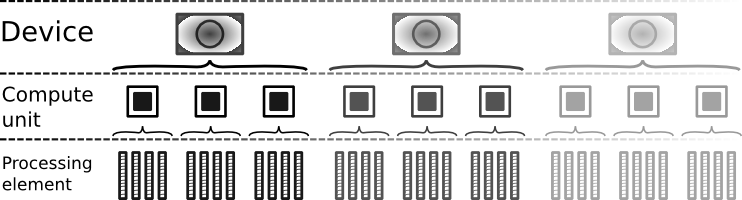
\includegraphics[scale=0.5]{../08-OpenCL/figs/platform.png}
\caption{The hierarchy defined by the OpenCL platform model.
A platform consists of multiple devices, each having multiple compute units. Whereas compute units can run independent threads, they can still contain multiple processing elements.
The memory model (\ref{sec:OpenCL:memmodel}) will also fit in this hierarchy, with (from the top) global, local and private memory residing close to corresponding layer.}
\label{fig:OpenCL:platform}
\end{center}
\end{figure}


\subsection{Execution model}
Code is written in its own language `.cl' which is a subset of the C99 standard, where functions callable from the host are called kernels.
This code is then compiled for an already initialized device, and submitted to a command queue.
The command queue is now responsible for running this kernel once the device is ready. 
It is possible to submit multiple kernels to a queue and manage their execution via events.

\paragraph*{}
Every time a kernel is queued, a virtual grid will be defined.
For every grid point, the kernel will be executed once.
This is how parallelism is achieved in OpenCL.
This so-called NDRange can be of one, two or three dimensions, and the size can be chosen arbitrarily up to a limit defined per device.

The entire global grid is divided into smaller local grids called work-groups.
An illustration of a 27x27 `2DRange' composed of nine 9x9 workgroups is found in figure~\ref{fig:OpenCL:ndrange}.
During execution each work-item will fill one processing element.
All work-items within the same work-group will run concurrently, but on the same compute unit. The other work-groups will run on other compute units within the same device.

\begin{figure}
\begin{center}
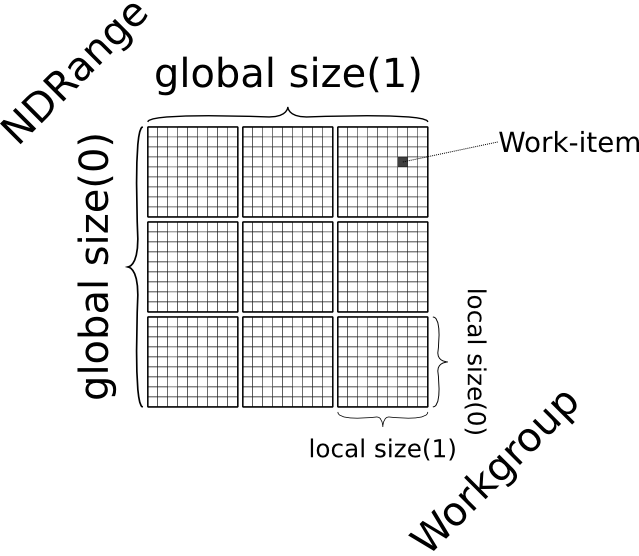
\includegraphics[scale=0.5]{../08-OpenCL/figs/NDRange.png}
\caption{A global two dimensional 27x27 NDRange. It is divided into nine work-groups, each having 9x9 work-items.}
\label{fig:OpenCL:ndrange}
\end{center}
\end{figure}



\subsection{Memory model}
\label{sec:OpenCL:memmodel}
There are four different regions for OpenCL memory:
\begin{itemize}
\item \textbf{Global} memory is allocated by the host. Both kernel and the host have read/write access. The slowest type of memory, but having a large memory size. Ideal for storing matrices or per work-item results.
\item \textbf{Constant} memory is allocated by the host, but kernels have read access only. Often used when passing many parameters/options as one struct to the kernel.
\item \textbf{Local} memory could be allocated either dynamically by the host or statically inside a kernel. Every work group share its own independent copy of this memory type. This memory is faster than global, because it resides close to each compute unit. 
\item \textbf{Private} memory is allocated statically by each work-item and not shared at all. Being closest to each processing item it is the fastest memory. Variables declared in kernels without specifying the region is private by default.
\end{itemize}
A quick summary of the different memory regions can be found in table~\ref{tab:OpenCL:memory}.

\begin{table}
\begin{center}
\begin{tabular}{c|cc|cc|cc|cc}
& \multicolumn{2}{c|}{Global} & \multicolumn{2}{c|}{Constant} & \multicolumn{2}{c|}{Local} & \multicolumn{2}{c}{Private}\\
& Host & Kernel& Host & Kernel& Host & Kernel& Host & Kernel \\
\hline
Allocation & Dyn & NA & Dyn & NA & Dyn & Stat & NA & Stat\\ 
Access & R/W & R/W & R/W & R & NA & R/W & NA & R/W\\ 
\hline 
\end{tabular} 
\caption{Overview of different OpenCL memory regions. R/W: read and write. R: read only. Dyn/Stat: dynamic/static. NA: not available.}
\label{tab:OpenCL:memory}
\end{center}
\end{table}



\subsection{Programming model}
OpenCL focuses on a data parallel programming model.
Here we have multiple memory objects that can be calculated or altered by the same set of instructions. 
Instead of using loops or nested loops, our problem can be simplified by choosing appropriate global and local sizes, as we shall see for general matrix multiplication in section~\ref{sec:OpenCL:matmult}.

Task parallel programming, and hybrids between these two, are also supported. 
GPUs however favors the data parallel model.




\section{GPU architecture}
\label{sec:OpenCL:GPUarchitecture}




\section{Matrix multiplication}
\label{sec:OpenCL:matmult}
The coupled cluster code has its bottleneck in matrix matrix multiplication.
Take for instance the second term of \eqref{eq:CC:t2eq},
\begin{equation}
t_{ij}^{ab} \leftarrow \frac{1}{2} \langle ab||de \rangle t^{de}_{ij} .
\end{equation}
Gathering indices $a,b \rightarrow \alpha$, $d,e \rightarrow \beta$ and finally $i,j \rightarrow \gamma$, it can be rewritten as
\begin{equation}
t_{\alpha,\gamma} \leftarrow \frac{1}{2} \sum_{\beta} \langle \alpha||\beta \rangle t_{\beta,\gamma} ,
\end{equation}
which is, apart from the factor $\frac{1}{2}$, identical to the mathematical definition of matrix multiplication,
\begin{equation}
C_{ij} = \sum_k A_{ik} B_{kj},
\hspace{10mm}
A \in \mathbf{R}^{m\times p}, B \in \mathbf{R}^{p\times n}, C \in \mathbf{R}^{m\times n}.
\end{equation}
Element $C_{ij}$ is thus the innerproduct of row $i$ in $A$ and column $j$ in $B$, as illustrated in fig.~\ref{fig:OpenCL:matmult}.


\begin{figure}
\begin{center}
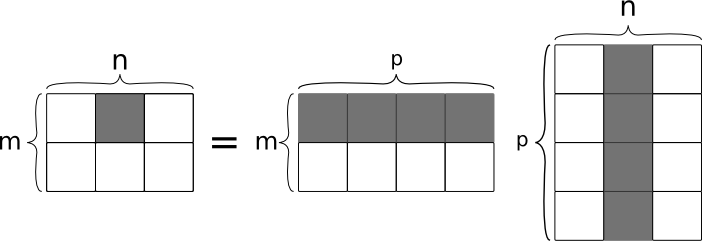
\includegraphics[scale=0.5]{../08-OpenCL/figs/matmult.png}
\caption{Outline of matrix multiplication, following its straight forward mathematical definition.}
\label{fig:OpenCL:matmult}
\end{center}
\end{figure}


\begin{figure}
\begin{center}
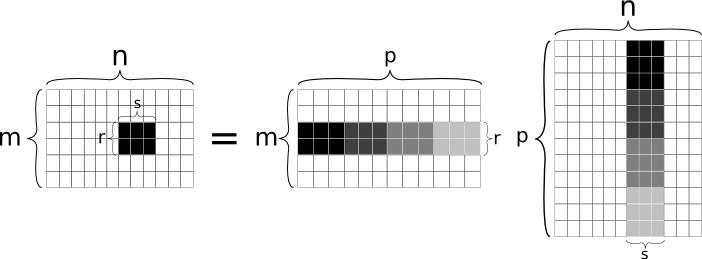
\includegraphics[scale=0.5]{../08-OpenCL/figs/matmult_loc.png}
\caption{Outline of blocked matrix multiplication.}
\label{fig:OpenCL:matmult_loc}
\end{center}
\end{figure}



\subsection{Strassen's algorithm}
The straight forward algorithm for matrix multiplication will require $p$ multiplications and $p-1$ additions for each of the $m\times n$ elements. The total number of floating point operations is then $mn(2p-1) \sim \mathcal{O}(mnp)$. If the matrices $A$ and $B$ can be divided into four equally sized blocks,
\begin{equation}
\begin{bmatrix}
C_{11} & C_{12} \\
C_{21} & C_{22}
\end{bmatrix}
=
\begin{bmatrix}
A_{11} & A_{12} \\
A_{21} & A_{22} 
\end{bmatrix}
\begin{bmatrix}
B_{11} & B_{12} \\
B_{21} & B_{22},
\end{bmatrix}
\end{equation}
which results in eight multiplications in total,
\begin{equation}
\begin{bmatrix}
C_{11} & C_{12} \\
C_{21} & C_{22}
\end{bmatrix}
=
\begin{bmatrix}
A_{11} B_{11} + A_{12} B_{21} & A_{11} B_{12} + A_{12} B_{22} \\
A_{21} B_{11} + A_{22} B_{21} & A_{21} B_{12} + A_{22} B_{22} 
\end{bmatrix}
.
\end{equation}



Defining some intermediates,
\begin{equation}
\label{eq:OpenCL:Strassen_intermediates}
\begin{matrix}
S_1 = A_{21} + A_{22}, & T_1 = B_{12} - B_{11},\\
S_2 = S_1 - A_{11}, & T_2 = B_{22} - T_1,\\
S_3 = A_{11} - A_{21}, & T_3 = B_{22} - B_{12},\\
S_4 = A_{12} - S_2, & T_4 = B_{21} - T_2 ,
\end{matrix}
\end{equation}
we only need seven multiplications,
\begin{equation}
\label{eq:OpenCL:Strassen_multiplications}
\begin{matrix}
P_1 &= A_{11} B_{11}, & U_1 = P_1 + P_2, \\
P_2 &= A_{12} B_{21}, & U_2 = P_1 + P_4, \\
P_3 &= S_1 T_1, & U_3 = U_2 + P_5,\\
P_4 &= S_2 T_2, & U_4 = U_3 + P_7,\\
P_5 &= S_3 T_3, & U_5 = U_3 + P_3,\\
P_6 &= S_4 B_{22}, & U_6 = U_2 + P_3,\\
P_7 &= A_{22} T_4, & U_7 = U_6 + P_6 ,
\end{matrix} 
\end{equation}
to find the resulting $C$ matrix as
\begin{equation}
\begin{bmatrix}
C_{11} & C_{12} \\
C_{21} & C_{22}
\end{bmatrix}
=
\begin{bmatrix}
U_1 & U_7 \\
U_4 & U_5 
\end{bmatrix}
.
\end{equation}


Despite the seemingly additional work, we have reduced the number of multiplications from 8 to 7. Since the multiplications are the computational bottleneck compared to addition and subtraction, the number of flops are reduced.

In the case of square $n\times n$ matrices with $n$ equal to a power of two, $n=2^m$, the divided blocks will have $\frac{n}{2} = 2^{m-1}$.
Letting the number of flops needed for the full matrix be $f(m)$ and applying Strassen recursively we find the total number of flops to be
\begin{equation}
f(m) = 7 f(m-1) = 7^2 f(m-2) = \cdots = 7^m f(0) , 
\end{equation}
where $f(0)$ is the one floating point operation needed for multiplication of two numbers (two $2^0\times 2^0$ matrices).
For large matrices this can prove extremely efficient, yielding a much better scaling, 
\begin{equation}
\mathcal{O}\left( 7^m \right) = 
\mathcal{O}\left( 2^{\log_2 7^m} \right) = 
\mathcal{O}\left( 2^{m \log_2 7} \right) = 
\mathcal{O}\left( n^{\log_2 7} \right) \approx
\mathcal{O}\left( n^{2.807} \right) ,
\end{equation}
effectively saving $7/8 = 12.5\%$ each time it is applied.






\section{Implementation}
Matrix multiplication has been considered an important aspect of this thesis, and all functionality has been implemented in a separate object called `GEMM' -- GEneral Matrix Multiplication.
The default implementation, demonstrated in listing~\ref{lst:OpenCL:GEMMdefault}, performs the matrix operation, 
\begin{equation}
C_{(res)} = \alpha A_{(left)} B_{(right)} + \beta C_{(res)} , 
\end{equation}
where the variable names used in the implementation are denoted in the subscript of the matrices.
When `transL' and/or `transR' is set true $A_{(left)}$ and/or $B_{(right)}$ will be transposed before used.
Armadillo's default operations will be used in `GEMM', most likely translated to calls to some BLAS library, Netlib~\cite{netlibblas} and GotoBLAS2~\cite{Goto:2008:HIL:1377603.1377607} being the two implementations tested for CPU here.
\begin{lstlisting}[float,label={lst:OpenCL:GEMMdefault},caption={GEMM default implementation.}]
virtual void dgemm(
        arma::mat &res,
        arma::mat const &left,
        arma::mat const &right,
        double alpha = 1,
        double beta = 0,
        bool transL = false,
        bool transR = false)
{
    timer.tic();
    if (transL == false && transR == false)
        res = alpha * left * right + beta * res;
    else if (transL == true && transR == false)
        res = alpha * trans(left) * right + beta * res;
    else if (transL == false && transR == true)
        res = alpha * left * trans(right) + beta * res;
    else if (transL == true && transR == true)
        res = alpha * trans(left) * trans(right) + beta * res;
    tot_time += timer.toc();

    return;
}
\end{lstlisting}

To take advantage of different implementations all C++ statements for matrix multiplication needs to be replaced with a call to a `GEMM' derived class.
As an example the second term from the coupled-cluster $\hat{T}_2$ equations, eq.~\ref{eq:CC:t2_t2_diag}, will now be written as 
\begin{equation}
\langle \xi | t'_2 | \mu \rangle_{(\lambda)} = \frac{1}{2} \sum_{\xi'} \langle \xi || \xi' \rangle_{(\lambda)} \langle \xi' |t_2| \mu \rangle_{(\lambda)} + 1 \langle \xi | t'_2 | \mu \rangle_{(\lambda)},
\end{equation}
with $\alpha = \frac{1}{2}$ and $\beta = 1$.
Implementing this listing~\ref{lst:CC:c_t2_t2} is altered slightly, as depicted in listing~\ref{lst:OpenCL:c_t2_t2}.
\begin{lstlisting}[float,label={lst:OpenCL:c_t2_t2},caption={Second term of the coupled-cluster $\hat{T}_2$ equations, now using the matrix-multiplication framework in `GEMM'.}]
for (int lmd = 0; lmd < basis->dim_lmd_2p(); lmd++)
    mult->dgemm(     //mult points to a GEMM derived object
       t2_new.at(lmd),              //Result
       sys->get_v_pppp()->at(lmd),  //Left
       t2_old.at(lmd),              //Right
       0.5, 1);                     //alpha, beta
\end{lstlisting}

Also incorporated is a system for tracking the amount of time that is used on multiplication.
A protected member, timer, of type `arma::wall\_clock', is included as well as a double, tot\_time, to record how much time is spent inside the `dgemm' method.
To extract this information one simply calls `get\_tot\_time()', returning the number of seconds elapsed.


\subsection{Strassen}
`Strassen' subclasses `GEMM' and adds the method,
\begin{lstlisting}
virtual arma::mat strassenMethod(
		const arma::mat& left,
		const arma::mat& right,
		int depth);
\end{lstlisting}
returning the product of `left' and `right' matrices.
Since the Strassen method is applied recursively, the first call should set `depth' to $0$, and it is raised by one each time a new level of recursion is performed.
This allows us to abort recursions at a specific level, helpful when timing whether blas routines or another level of recursion is the most beneficial for a specific size of the matrices.

The `dgemm' function is overridden as in listing~\ref{lst:OpenCL:Strassen_dgemm}, essentially the same as for the default base-class implementation except multiplying with the new `strassenMethod'.
\begin{lstlisting}[float,label={lst:OpenCL:Strassen_dgemm},caption={Strassen overrides the `dgemm' method.}]
timer.tic();
if (transL == false && transR == false)
  res = alpha * strassenMethod(left, right, 0) 
       + beta * res;
else if (transL == true && transR == false)
  res = alpha * strassenMethod(trans(left), right, 0) 
       + beta * res;
else if (transL == false && transR == true)
  res = alpha * strassenMethod(left, trans(right), 0) 
       + beta * res;
else if (transL == true && transR == true)
  res = alpha * strassenMethod(trans(left), trans(right), 0) 
  	   + beta * res;
tot_time += timer.toc();

return;
\end{lstlisting}
In `strassenMethod' the criterion for adding one level of recursion or invoking an underlying blas library is 
\begin{equation}
3 m n p < \tau \left( mn + np + pm \right),
\end{equation}
reduced to 
\begin{equation}
n < \tau
\end{equation}
in the case of equally sized square matrices, $m=n=p$.
Such a criterion was first proposed by Higham in 1990~\cite{Higham:1990:EFM:98267.98290}.
Other criteria exist but this was chosen because only one variable, $\tau$, needs to be tuned.
We estimate $\tau$ empirically by measuring the time a regular `dgemm' routine uses compared to doing one Strassen recursion for different sizes $m, n$ and $p$.


The first part of `strassenMethod', listing~\ref{lst:OpenCL:Strassen_p1}, defines some integer values needed, `m', `n' and `p' hold the size of the matrices, and `m2', `n2' and `p2' store half their size.
`dp1' is the current recursion level plus one.
If one of the dimensions is less than two it is not possible to split the matrices further, and if the recursion criterion is not met it has no benefit to split the matrices further.
These conditions are tested for, and regular multiplication through armadillo will then be used instead.
\begin{lstlisting}[float,label={lst:OpenCL:Strassen_p1},caption={Strassen p1},name={strassen_complete}]
//Needed integer values
int m = left.n_rows;
int m2 = m / 2;
int n = right.n_cols;
int n2 = n / 2;
int p = left.n_cols;
int p2 = p / 2;
int dp1 = depth + 1;

//Criterion for further recursion. Tau is a class member (double)
if (m < 2 || n < 2 || p < 2 || (3.0 * m * n * p) / (((double) n) * p + ((double) m) * n + ((double) m) * p) < tau)
{
  return left * right;
}
\end{lstlisting}


The second part, in listing~\ref{lst:OpenCL:Strassen_p2}, deals with situations where matrices may have odd dimensions, and thus not suitable for the Strassen algorithm.
We deal with these situations using dynamic peeling, taking away the odd rows and columns, 
\begin{equation}
\begin{bmatrix}
C_{11}  & c_{12} \\
c_{21}  & c_{22}
\end{bmatrix}
=
\begin{bmatrix}
A_{11} & a_{12} \\
a_{21} & a_{22} 
\end{bmatrix}
\begin{bmatrix}
B_{11} & b_{12} \\
b_{21} & b_{22} 
\end{bmatrix}
= 
\begin{bmatrix}
A_{11}B_{11} + a_{12}b_{21}  & A_{11}b_{12} + a_{12}b_{22} \\
a_{21}B_{11} + a_{22}b_{21}  & a_{21}b_{12} + a_{22}b_{22} 
\end{bmatrix} , 
\end{equation}
where $A_{11}$, $B_{11}$ and $C_{11}$ now are the largest possible blocks with even dimensions.
We then have one multiplication,
\begin{equation}
C_{11} = A_{11}B_{11} , 
\end{equation}
suitable for another level of Strassen, and in the end a few fix-up steps,
\begin{equation}
\begin{split}
C_{11} =&  a_{12}b_{21}  + C_{11} \\
c_{12} =& A_{11}b_{12} + a_{12}b_{22} \\
c_{21} =& a_{21}B_{11} + a_{22}b_{21} \\
c_{22} =& a_{21}b_{12} + a_{22}b_{22} ,
\end{split}
\end{equation}
where all steps may not be applicable if only some of the dimensions are odd.
\begin{lstlisting}[float,label={lst:OpenCL:Strassen_p2},caption={Strassen p2. Continuation of listing~\ref{lst:OpenCL:Strassen_p1}.},name={strassen_complete}]
else if (m % 2 != 0 || n % 2 != 0 || p % 2 != 0) 
{
  span m2Div2(0, m2 * 2 - 1); //Spanning all elements
  span n2Div2(0, n2 * 2 - 1); //except the last, if
  span p2Div2(0, p2 * 2 - 1); //the total number is odd.
  span lastM(m - 1, m - 1); //Spanning 
  span lastN(n - 1, n - 1); //the last
  span lastP(p - 1, p - 1); //element.

  mat C(m, n);
  C(m2Div2, n2Div2) = strassenMethod(left(m2Div2, p2Div2), right(p2Div2, n2Div2), depth);

  if (p % 2 != 0) //C_11 += a_12 b_21
    C(m2Div2, n2Div2) += left(m2Div2, lastP) * right(lastP, n2Div2);

  if (n % 2 != 0)
  {	//c_12 = A_11 b_12
    C(m2Div2, lastN) = left(m2Div2, p2Div2) * right(p2Div2, lastN);

    if (p % 2 != 0)  //c_12 += a_12 b_22
      C(m2Div2, lastN) += left(m2Div2, lastP) * right(lastP, lastN);        
  }

  if (m % 2 != 0)
  {	//c_21 = a_21 B_11
    C(lastM, n2Div2) = left(lastM, p2Div2) * right(p2Div2, n2Div2);

    if (p % 2 != 0)  //c_21 += a_22 b_21
      C(lastM, n2Div2) += left(lastM, lastP) * right(lastP, n2Div2);
  }

  if (m % 2 != 0 && n % 2 != 0)
  {	//c_22 = a_21 b_12
    C(lastM, lastN) = left(lastM, p2Div2) * right(p2Div2, lastN);

    if (p % 2 != 0)  //c_22 += a_22 b_22
      C(lastM, lastN) += left(lastM, lastP) * right(lastP, lastN);
  }

  return C;
}
\end{lstlisting}






The third and last part of our Strassen implementation, listing~\ref{lst:OpenCL:Strassen_p3}, carries out the actual Strassen algorithm, implemented straight forward from the equations~\eqref{eq:OpenCL:Strassen_intermediates} and~\eqref{eq:OpenCL:Strassen_multiplications}.
\begin{lstlisting}[float,label={lst:OpenCL:Strassen_p3},caption={Strassen p3. Continuation of listing~\ref{lst:OpenCL:Strassen_p2}.},name={strassen_complete}]
else
{
 //left matrix
 span lR1(0, m2 - 1); //First half of rows
 span lR2(m2, m - 1); //Second half of rows
 span lC1(0, p2 - 1); //First half of columns
 span lC2(p2, p - 1); //Second half of columns
 //right matrix
 span rR1(0, p2 - 1); //First half of rows
 span rR2(p2, p - 1); //Second half of rows
 span rC1(0, n2 - 1); //First half of columns
 span rC2(n2, n - 1); //Second half of columns

 //Intermediates
 mat S1 = left(lR2, lC1) + left(lR2, lC2);
 mat S2 = S1 - left(lR1, lC1);
 mat S3 = left(lR1, lC1) - left(lR2, lC1);
 mat S4 = left(lR1, lC2) - S2;
 mat T1 = right(rR1, rC2) - right(rR1, rC1);
 mat T2 = right(rR2, rC2) - T1;
 mat T3 = right(rR2, rC2) - right(rR1, rC2);
 mat T4 = right(rR2, rC1) - T2;

 //Multiplications
 mat P1 = strassenMethod(left(lR1,lC1), right(rR1,rC1), dp1);
 mat P2 = strassenMethod(left(lR1,lC2), right(rR2,rC1), dp1);
 mat P3 = strassenMethod(S1, T1, dp1);
 mat P4 = strassenMethod(S2, T2, dp1);
 mat P5 = strassenMethod(S3, T3, dp1);
 mat P6 = strassenMethod(S4, right(rR2, rC2), dp1);
 mat P7 = strassenMethod(left(lR2, lC2), T4, dp1);

 //U matrices
 mat U1 = P1 + P2;
 mat U2 = P1 + P4;
 mat U3 = U2 + P5;
 mat U4 = U3 + P7;
 mat U5 = U3 + P3;
 mat U6 = U2 + P3;
 mat U7 = U6 + P6;

 //Fill and return the result
 mat C(m, n);
 C(lR1, rC1) = U1;
 C(lR1, rC2) = U7;
 C(lR2, rC1) = U4;
 C(lR2, rC2) = U5;
 return C;
}
\end{lstlisting}







\subsection{CLgemm}
Matrix multiplication on GPUs through OpenCL is managed by AMD's own library APPML (Accelerated Parallel Processing Math Libraries).
Again the `dgemm' method is altered to use a function for the product itself, this time implemented in `clmult'.

The overhead when using GPUs is substantial, and we need to empirically find where a CPU implementation is more efficient.
We have chosen the simplest criterion, whenever the amount of floating point operations needed is less than a threshold value, armadillo's underlying functionality is used instead.
In listing~\ref{lst:OpenCL:CLgemm_p1} we see how one can find the number of flops required and decide whether the CPU or GPU is suited.
If there is enough work to be done data will be pushed to the graphics card followed by invoking the routine `clAmdBlasDgemm' to calculate the matrix product, as shown in listing~\ref{lst:OpenCL:CLgemm_p2}.

\begin{lstlisting}[float,label={lst:OpenCL:CLgemm_p1},caption={CLgemm multiplication implementation.},name={CLgemm}]
mat CLgemm::clmult(mat const &left, mat const &right) {

int m = left.n_rows;  //Size 
int n = right.n_cols; //of input
int p = left.n_cols;  //matrices.

mat res = zeros<mat > (m, n); //Result

//Flops ~O(mnp)
double work = ((double) m) * n * p;

//Don't use GPU if few flops are required. Found 
//empirically by testing where GPUs are quicker than CPUs.
if (work < 3e8)
  res = left * right;
\end{lstlisting}
\begin{lstlisting}[float,label={lst:OpenCL:CLgemm_p2},caption={CLgemm multiplication implementation. Continuation of listing~\ref{lst:OpenCL:CLgemm_p1}},name={CLgemm}]    
else
{
  //memptr can't be const in cl.
  cl_double *A_p = const_cast<double *> (left.memptr());
  cl_double *B_p = const_cast<double *> (right.memptr());
  cl_double *C_p = res.memptr();
  
  //Create CL buffers, copying Host memory.
  cl::Buffer A_cl(context, CL_MEM_READ_ONLY | CL_MEM_COPY_HOST_PTR, sizeof (*A_p) * left.n_elem, A_p);
  cl::Buffer B_cl(context, CL_MEM_READ_ONLY | CL_MEM_COPY_HOST_PTR, sizeof (*B_p) * right.n_elem, B_p);
  cl::Buffer C_cl(context, CL_MEM_READ_WRITE | CL_MEM_COPY_HOST_PTR, sizeof (*C_p) * res.n_elem, C_p);
 
  //Run DGEMM. armadillo uses columnmajor ordering.
  clAmdBlasDgemm( 
    clAmdBlasColumnMajor, clAmdBlasNoTrans, clAmdBlasNoTrans,
    m, n, p,      //Size of matrices.
    1.0, A_cl(), m, B_cl(), p,
    0.0, C_cl(), m,
    1, &queue(), 0, NULL, NULL);
  
  //Read results back into C
  queue.enqueueReadBuffer(C_cl, true, 0, sizeof (*C_p) * res.n_elem, C_p); 
}

return res;
}//End Method CLgemm::clmult
\end{lstlisting}








\subsection{CLstrassen}
Our `CLgemm' implementations will meet severe problems as the matrix size increases, the device will run out of available memory. 
Solving this, the matrix needs to be partitioned into smaller blocks that can be processed one at a time.
For large matrices we also experience that applying Strassen with AMD's APPML as blas back-end serves no purpose, the GPU is more efficient than the overhead of blocking up the matrices.

For these reasons we have combined `Strassen' and `CLgemm', using the Strassen algorithm with a modified criterion, now only applying another level of recursion until the blocks are small enough to fit on the GPU.
The new criterion is described by listing~\ref{lst:OpenCL:CLstrassen_criterion}, and the parameter `maxSizeCL' is found in listing~\ref{lst:OpenCL:CLstrassen_maxSizeCL}.
\begin{lstlisting}[float,label={lst:OpenCL:CLstrassen_criterion},caption={CLstrassen's new criterion.}]
int m = left.n_rows;
int m2 = m / 2;
int n = right.n_cols;
int n2 = n / 2;
int p = left.n_cols;
int p2 = p / 2;

//Number of elements in the three matrices
size_t sizRes = m * n;
size_t sizLeft = m * p;
size_t sizRight = n * p;
size_t sizTOT = sizRes + sizRight + sizLeft;
//Number of bytes needed
sizTOT = sizeof (double) * sizTOT;

//Matrix small enough for Device?
if (sizTOT < maxSizeCL)
  return clmult.clmult(left, right); 
\end{lstlisting}
\begin{lstlisting}[float,label={lst:OpenCL:CLstrassen_maxSizeCL},caption={How to query the max number of bytes on a GPU device available for OpenCL.}]
cl_ulong maxmem_bytes = device.getInfo<CL_DEVICE_MAX_MEM_ALLOC_SIZE > ();
maxSizeCL = 0.9 * maxmem_bytes;
\end{lstlisting}














\part{Results}
\chapter{Selected Results} \label{chp:results}
\epigraph{Results! Why, man, I have gotten a lot of results. I know several thousand things that won't work.}{Thomas A. Edison, \cite{noauthor_edisonian_nodate}}
\begin{figure}[H]
	\centering
	\includegraphics[scale=0.6]{../Images/art.eps}
	\caption{Radial one-body density profiles for two-dimensional quantum dots with $N=12$ electrons, popularly titled an artificial Magnesium atom. The four graphs correspond to four different oscillator frequencies, where the weakest oscillator gives the broadest density distribution. It's quite artistic, isn't it?}
\end{figure}

We are finally ready to discuss the most exciting part of this thesis, namely the results. Since this work, after all, is about physics, the physical insight should be our focus and in this chapter we finally get the opportunity to discuss pure physics. However, we will also use this section for the comparison of the restricted Boltzmann machine (RBM) and the standard variational Monte Carlo method (VMC) to decide which one that is the better and in which situations they differ. We will look at three versions of the RBM; a Slater determinant with the Boltzmann machines as the single-particle functions (RBM), as described in chapter \ref{chp:rbmimplementation}, an RBM with the simple Jastrow factor described in section \ref{sec:rbmsj} (RBM+SJ) and an RBM with the Padé-Jastrow factor described in section \ref{sec:jastrow} (RBM+PJ). For VMC, we use the Slater-Jastrow ansatz, i.e., the trial wave function consists of a Padé-Jastrow factor and a Slater determinant containing standard single-particle functions, as detailed in chapter \ref{chp:WFE}. 

As we are capable of studying various systems, system sizes $N$, system strengths $\omega$, and innumerous hyper-parameter settings by different methods, the number of results we are able to produce is uncountable. In total, we have looked at more than 150 different quantum dot systems using the four methods mentioned above, which means that we have generated a large set of results. Just a small subset of those results will be presented and discussed in this chapter, while a more extensive collection of results is presented in appendix \ref{chp:totalresults}. The results presented below were selected since they describe physically interesting properties and compare the various methods in an informative way. Typically, we will choose systems and configurations that are comparable to references, such that we can benchmark the results. Our primary focus will be on ground state energy and electron density calculations, and we will stick to natural units as discussed in appendix \ref{app:units}. A brief recap is that for quantum dots, the energy is given in units of Planck's reduced constant, $E'=E/\hbar$, length is scaled as $x'=x/\sqrt{\hbar/m}$ where $m$ is the mass of a particle, which implies that the $d$-dimensional density, $\rho_d(\bs{r})$, is given in units of $(\hbar/m)^{-d/2}$. For atoms, we use Hartree atomic units, meaning that the length is given in units of the Bohr radius, $a_0$, the $d$-dimensional density is given in units of $a_0^{-d}$ and the energy is scaled as $E'=E/(\hbar^2/m_ea_0)$.

Before we move on to the physical results, we will take a quick look at some more technical results, more precisely the computational cost of various wave function structures and the energy convergence using various optimization tools. For validation purposes, we will present a few selected results on the case without repulsive interaction and compare it to analytical results. After that, we study the case with repulsive interaction on a much larger scale, where we first look at quantum dots and then on double atoms.

\begin{figure}
	\centering 
	% This file was created by matplotlib2tikz v0.7.4.
\begin{tikzpicture}[scale=0.9]

\begin{axis}[name=2D, xlabel=$N$, ylabel={CPU-time [s]}, grid=major, 
legend cell align={left},
legend style={at={(1.68,1.10)}, anchor=south east, draw=white!80.0!black},
legend columns = 6, 
clip=false,
xtick=data] 
\addplot[color=color0,mark=oplus*, dashed] coordinates { 
	(2,6.05)
	(6,11.25)
	(12,20.53) 
	(20,38.99) 
	(30,73.73) 
	(42,130.49) 
	(56,213.47)
	(72,360.22)
	(90,856.84) }; 
\addlegendentry{RBM};

\addplot[color=color1,mark=oplus*, dash dot] coordinates { 
	(2,7.12) 
	(6,14.07) 
	(12,28.42) 
	(20,63.27) 
	(30,122.93) 
	(42,199.60)
	(56,349.22)}; 
\addlegendentry{RBM+SJ};

\addplot[color=color2,mark=oplus*, dotted] coordinates { 
	(2,7.26)
	(6,13.50)
	(12,27.68)
	(20,57.09) 
	(30,119.17) 
	(42,212.53) 
	(56,382.13) }; 
\addlegendentry{RBM+PJ};

\addplot[color=color3,mark=oplus*] coordinates { 
	(2,5.11)
	(6,10.51)
	(12,20.85) 
	(20,41.20) 
	(30,76.26) 
	(42,137.39) 
	(56,230.63)
	(72,355.81)
	(90,544.03) }; 
\addlegendentry{VMC};

\node[] at (axis cs: 44,978) {2D};
\end{axis}

\begin{axis}[name=2D, 
xshift=7.9cm, 
xlabel=$N$, 
grid=major, 
clip=false,
xtick=data] 
\addplot[color=color0,mark=oplus*, dashed] coordinates { 
	(2,7.69)
	(8,20.92)
	(20,59.67) 
	(40,171.84) 
	(70,586.39) }; 
%\addlegendentry{RBM};

\addplot[color=color1,mark=oplus*, dash dot] coordinates { 
	(2,8.95)
	(8,26.86)
	(20,94.64) 
	(40,270.92) }; 
%\addlegendentry{RBM+SJ};

\addplot[color=color2,mark=oplus*, dotted] coordinates { 
	(2,8.87)
	(8,26.36)
	(20,91.40) 
	(40,293.25) }; 
%\addlegendentry{RBM+PJ};

\addplot[color=color3,mark=oplus*] coordinates { 
	(2,6.70)
	(8,20.99)
	(20,62.54) 
	(40,185.65) 
	(70,486.02) };
%\addlegendentry{VMC};

\node[] at (axis cs: 35,670) {3D};
\end{axis}
\end{tikzpicture}
	\caption{CPU-time per iteration for $M=2^{20}=1,048,576$ cycles as a function of the number of electrons, N, for two- dimensional (left) and three-dimensional (right) quantum dots. Table with numbers and more information about simulations can be found in appendix \ref{chp:totalresults}, section \ref{sec:cputime}. For abbreviations see the text.}
	\label{fig:cpu_time}
\end{figure} 

\section{Computational cost}
Many-body quantum simulations are frequently found on lists of the most computationally expensive simulations for scientific purposes, which is caused by the large amount of information that is stored in the wave function. Albeit the VMC method is known to have a high performance-cost ratio, it is still not cheap. In this section, we will find the average cost of VMC and compare it to the cost of the RBM methods described above. In figure \eqref{fig:cpu_time}, the CPU-time is plotted as a function of the number of electrons for two-dimensional (left) and three-dimensional (right) quantum dots. To obtain accurate CPU-times, all the simulations were run on the Abel computer cluster with $M=2^{20}=1,048,576$ Monte Carlo cycles per iteration. The time presented is the average time over at least four independent runs with thousands of iterations each. To see the actual numbers that the plots are based on, go to appendix \ref{chp:totalresults}, section \ref{sec:cputime}. 

Our immediate observation is that the methods are pairwise quite similar, with RBM and VMC as the cheapest methods, and RBM+SJ and RBM+PJ as the most expensive ones. This is not surprising, as the RBM requires a neural network, VMC requires a Jastrow factor while RBM+SJ and RBM+SJ requires both a neural network and a Jastrow factor. For two-dimensional dots, the RBM is the cheapest among all the methods, but for larger systems ($N=42,56$ with $N$ as the number of electrons), VMC gets cheaper due to an explosion in CPU-time for the RBM. This explosion can be explained by our choice of the number of hidden nodes, $H$, which consequently is set to the number of electrons, i.e., $H=N$, which by \citet{nordhagen_computational_2018} was found to give the lowest energy for small quantum dots. Since the RBM has $N\cdot d\cdot (1+H)+H$ variational parameters with $d$ as the number of dimensions, the number of variational parameters for a two-dimensional dot with $N=90$ electrons is 16,470! On the other hand, the VMC method is equipped with two variational parameters for all system sizes, which obviously make the parameter update less costly. We also observe that the RBM+PJ is cheaper than the RBM+SJ for systems up to $N=42$, but after that, the RBM+SJ gets slightly cheaper. This might be surprising, as the simple Jastrow contains $N^2$ variational parameters, but a possible explanation is that BLAS is optimized for large matrix-vector operations and is thus fully utilized first when the matrices get large. We observe the same behavior for the three-dimensional dots as for the two-dimensional dots, and the discussion above is representative for them as well.

The standard way of estimating the scaling of a VMC algorithm is to fit the power function $f(x)=ax^b$ to the cost graph. As all the simulations were performed with the same hyper-parameters and with equal external factors, we fix the first parameter $a$ and focus on the second parameter $b$ only. It is this latter parameter that specifies the scaling, i.e.; we say that the method scales as $N^b$. For comparison reasons, we set $a=0.5$ as this was found to be a good average value. In table \eqref{tab:cputimefit}, the optimal $b$ from linear regression is presented for our four methods in two and three dimensions. We want to emphasize that we only did the regression for CPU-times up to $N=56$ in two dimensions and $N=40$ in three dimensions, partly because we only have data for all methods in this interval and partly because the CPU-time for the RBM explodes for large dots. We believe that this was the best way to do it in order to make the various methods comparable. 

\begin{table}
	\caption{The scaling of the computational cost of two-dimensional (2D) and three-dimensional (3D) quantum dots as a function of the number of electrons. The numbers presented in the table are the optimal $b$-value found fitting the power function $f(N)=0.5N^b$ to the cost graph. For abbreviations see the text.}
	\begin{tabularx}{\textwidth}{CCCCC} \hline\hline
		\label{tab:cputimefit}
		\makecell{\\ \phantom{=}} & RBM & RBM+SJ & RBM+PJ & VMC \\ \hline \\
		2D & 1.498 & 1.639 & 1.621 & 1.515 \\ 
		3D & 1.584 & 1.710 & 1.729 & 1.605 \\ \hline\hline
	\end{tabularx}
\end{table}

The numbers in the table match our impression from figure \eqref{fig:cpu_time}, where RBM and VMC pairwise were found to be more expensive than RBM+SJ and RBM+PJ. For all the methods, the scaling was found to be between linear and quadratic as a function of the number of electrons, which is surprising as the update of the Slater matrix scales as $\sim N^2$. 

\section{Energy convergence}
We want our calculations to converge fast and to be stable, and that is what the optimization tool is responsible for. In figure \eqref{fig:convergenceoptimization}, we compare standard gradient descent (GD) to stochastic gradient descent (SGD) and ADAM for quantum dots with $N=2$ interacting electrons in two and three dimensions. The optimization algorithms were detailed in section \ref{sec:optimizationalgorithms}. The gradient descent methods are plain, i.e., without momentum and adaptive learning rate, while the ADAM optimizer has momentum and adaptivity by nature. The frequency $\omega=1.0$ is used for the two-dimensional case since we know that the exact energy is $E=3.0$ for this case \cite{taut_two_1993}. Similarly, we use the frequency $\omega=0.5$ for the three-dimensional case since the exact energy is $E=2.0$ \cite{taut_two_1994}. 

\begin{figure}
	\centering 
	\subfloat{{\begin{tikzpicture} [scale=0.9, spy using outlines=
	{rectangle, magnification=8,size=2cm, height=1cm, connect spies}]
	\begin{axis} [name=2D, 
	xlabel=Iteration, 
	ylabel={$E/\hbar$}, 
	grid=major, 
	clip=false,
	every axis plot/.append style={thick},
	legend cell align={left},
	legend style={at={(1.45,1.1)}, anchor=south east, draw=white!80.0!black},
	legend columns = 6
	]
	
	\addplot[color2] table [x expr=\coordindex+1, 
	y index=0, 
	mark=none] {../data/GD_2D_MC16777216.dat};
	\addlegendentry{GD};
	
	\addplot[color1] table [x expr=\coordindex+1, 
	y index=0, 
	mark=none] {../data/SGD_2D_MC16777216.dat}; 
	\addlegendentry{SGD};
	
	\addplot[color0] table [x expr=\coordindex+1, 
	y index=0, 
	mark=none, 
	color=blue] {../data/ADAM_2D_MC16777216.dat}; 
	\addlegendentry{ADAM};
	
	\addplot [dashed,mark=none,black] coordinates {(0,3) (100,3)};
	\addlegendentry{Exact};
	
	\node[] at (axis cs: 50,3.178) {2D, $\omega=1.0$};
	\coordinate (spypoint1) at (axis cs:75,2.995001);
	\coordinate (magnifyglass1) at (axis cs:50,3.1);
	\end{axis}
	\spy [size=2.0cm] on (spypoint1)
	in node[fill=white] at (magnifyglass1);
	
	\begin{axis} [name=3D, 
	xshift=7.9cm, 
	xlabel=Iteration, 
	grid=major, 
	clip=false,
	every axis plot/.append style={thick}]	
	\addplot[color2] table[x expr=\coordindex+1, y index=0, mark=none] {../data/GD_3D_MC16777216.dat};  
	%\addlegendentry{GD};
	
	\addplot[color1] table[x expr=\coordindex+1, y index=0, mark=none] {../data/SGD_3D_MC16777216.dat};  
	%\addlegendentry{SGD};
	
	\addplot[color0] table[x expr=\coordindex+1, y index=0, mark=none] {../data/ADAM_3D_MC16777216.dat}; 
	%\addlegendentry{ADAM};
	
	\addplot+ [dashed,mark=none,color=black] coordinates {(0,2) (100,2)};
	%\addlegendentry{Exact};
	
	\node[] at (axis cs: 50,2.1355) {3D, $\omega=0.5$};
	\coordinate (spypoint2) at (axis cs:75,1.997);
	\coordinate (magnifyglass2) at (axis cs:50,2.077);
	\end{axis} 
	\spy [size=2.0cm] on (spypoint2)
	in node[fill=white] at (magnifyglass2);
\end{tikzpicture}}}
	\caption{Convergence of estimated ground state energy, $E$, for quantum dots with $N=2$ calculated using the VMC method, detailed in the text. We compare the optimization tools gradient descent (GD), stochastic gradient descent with 10 batches (SGD) and the ADAM optimizer. The left-hand side plot shows a two-dimensional quantum dot of frequency $\omega=1.0$ with exact energy $E=3.0$ \cite{taut_two_1993}. The right-hand side plot shows a three-dimensional quantum dot of frequency $\omega=0.5$ with exact energy $E=2.0$ \cite{taut_two_1994}. The learning rate was set to $\eta=0.5$ and the number of Metropolis steps was $M=2^{24}=16,777,216$. All energies are given in units of $\hbar$ (natural units).}
	\label{fig:convergenceoptimization}
\end{figure} 

The first thing we observe is that all three optimization tools manage to converge to the exact energy (see spy window). The stochastic and non-stochastic gradient descent methods behave similarly, but we observe that the SGD goes below the exact energy before it stabilizes. The ADAM optimizer, on the other hand, fluctuates much more, which can be described by the momentum, as discussed in section \ref{sec:momentum}. It is also important to remember that we use VMC, which is equipped with two variational parameters only, and thus is easier to control. The ADAM optimizer is known to be good at machine learning problems where we have many variational parameters, so we will stick to it even though gradient descent seems like a clever choice seen from the figure. Another point is that the circular quantum dots have neat potentials without local minima. When we move on to more complex systems, ADAM generally works better according to the literature.

\begin{figure}
	\centering 
	\subfloat{{% This file was created by tikzplotlib v0.8.1.
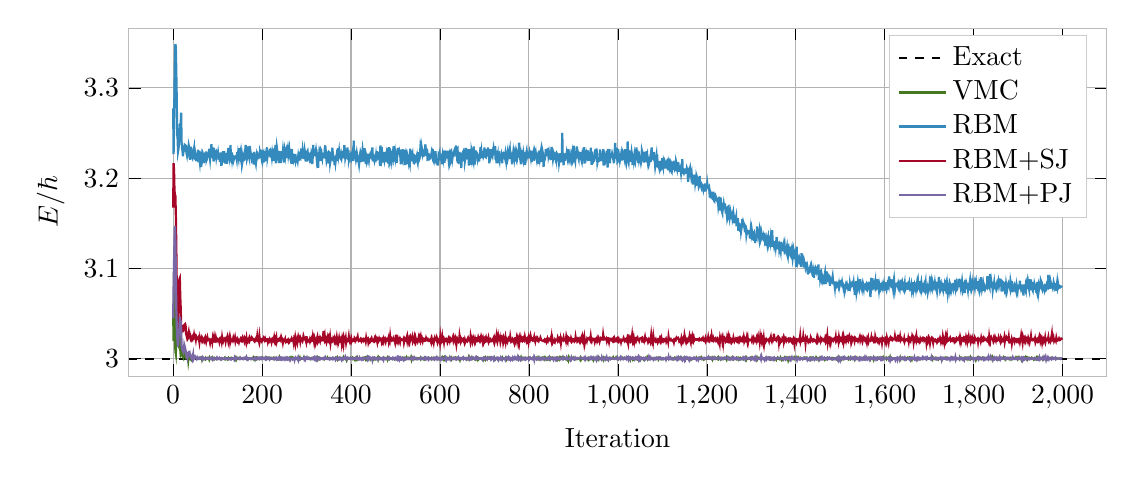
\begin{tikzpicture}

\definecolor{color0}{rgb}{0.203921568627451,0.541176470588235,0.741176470588235}
\definecolor{color1}{rgb}{0.650980392156863,0.0235294117647059,0.156862745098039}
\definecolor{color2}{rgb}{0.47843137254902,0.407843137254902,0.650980392156863}
\definecolor{color3}{rgb}{0.274509803921569,0.470588235294118,0.129411764705882}

\begin{axis}[
axis line style={white!73.72549019607844!black},
legend cell align={left},
legend style={draw=white!80.0!black},
tick pos=both,
x grid style={white!69.80392156862744!black},
xlabel={Iteration},
xmajorgrids,
xmin=-99.9499999999999, xmax=2098.95,
width=14cm,
height=6cm,
xtick style={color=black},
y grid style={white!69.80392156862744!black},
ylabel={$E/\hbar$},
ymajorgrids,
ymin=2.9807755, ymax=3.3660945,
ytick style={color=black}
]
\addplot [thick, black, dashed]
table {%
-99.9499999999999 3
2098.95 3
};
\addlegendentry{Exact}
\addplot [thick, color3]
table {%
-1.98991768347129e-15 3.04959
0.999999999999998 3.01958
2 3.09682
3 3.08172
4 3.04253
5 3.0082
6 3.00532
7 3.02106
8 3.03036
9 3.03826
10 3.02706
11 3.01589
12 3.01468
13 3.02001
14 3.03229
15 3.02307
16 3.00997
17 3.00401
18 3.00495
19 3.0102
20 3.00783
21 3.0048
22 3.002
23 3.00101
24 3.00527
24.9999999999995 3.00544
25.9999999999995 3.00456
26.9999999999995 3.00586
27.9999999999994 3.00346
28.9999999999994 3.00136
29.9999999999994 3.00207
30.9999999999994 3.00605
31.9999999999994 3.00601
32.9999999999993 3.00376
33.9999999999993 2.9984
34.9999999999993 3.00272
35.9999999999993 3.00149
36.9999999999993 3.00122
37.9999999999992 3.00043
38.9999999999992 3.0019
39.9999999999992 3.00017
40.9999999999992 2.99925
41.9999999999992 3.00079
42.9999999999991 3.0015
43.9999999999991 3.00268
44.9999999999991 3.00125
45.9999999999991 3.00077
46.9999999999991 3.00108
47.999999999999 3.00081
48.999999999999 3.00069
49.999999999999 3.0012
50.999999999999 3.00091
51.999999999999 3.00107
52.9999999999989 3.00045
53.9999999999989 3.00096
54.9999999999989 3.00126
55.9999999999989 3.00055
56.9999999999989 3.00051
57.9999999999988 3.00077
58.9999999999988 3.00047
59.9999999999988 2.99992
60.9999999999988 3.00023
61.9999999999988 3.00115
62.9999999999987 3.00086
63.9999999999987 3.0013
64.9999999999987 2.99916
65.9999999999987 3.00076
66.9999999999987 3.00077
67.9999999999986 2.99959
68.9999999999986 2.99972
69.9999999999986 3.00035
70.9999999999986 3.0005
71.9999999999986 2.99972
72.9999999999985 3.00071
73.9999999999985 2.99981
74.9999999999985 3.00037
75.9999999999985 3.00064
76.9999999999985 3.001
77.9999999999984 3.0008
78.9999999999984 3.00024
79.9999999999984 3.00066
80.9999999999984 2.99937
81.9999999999984 3.00116
82.9999999999983 3.00023
83.9999999999983 3.00099
84.9999999999983 3.00101
85.9999999999983 3.00018
86.9999999999983 2.99954
87.9999999999982 2.99974
88.9999999999982 3.00119
89.9999999999982 3.00059
90.9999999999982 3.00008
91.9999999999982 2.99958
92.9999999999982 3.00056
93.9999999999981 2.99999
94.9999999999981 3.00059
95.9999999999981 3.00049
96.9999999999981 3.00068
97.999999999998 3.00095
98.999999999998 3.0011
99.999999999998 3.00066
100.999999999998 2.99999
101.999999999998 3.0002
102.999999999998 2.99977
103.999999999998 2.99986
104.999999999998 2.99996
105.999999999998 2.99957
106.999999999998 3.00038
107.999999999998 3.00063
108.999999999998 3.00069
109.999999999998 3.00033
110.999999999998 3.00007
111.999999999998 2.99969
112.999999999998 2.99967
113.999999999998 2.99986
114.999999999998 3.00042
115.999999999998 3.00102
116.999999999998 2.99985
117.999999999998 3.00066
118.999999999998 3.00076
119.999999999998 3.00062
120.999999999998 3.00065
121.999999999998 2.99976
122.999999999998 3.00064
123.999999999998 3.00107
124.999999999998 2.99983
125.999999999997 3.00025
126.999999999997 3.00057
127.999999999997 3.00052
128.999999999997 3.00074
129.999999999997 3.001
130.999999999997 3.00044
131.999999999997 3.0009
132.999999999997 3.00051
133.999999999997 3.00059
134.999999999997 3.00068
135.999999999997 3.00059
136.999999999997 3.00024
137.999999999997 3.00033
138.999999999997 3.00023
139.999999999997 2.99941
140.999999999997 3.00082
141.999999999997 2.99928
142.999999999997 3.0004
143.999999999997 3.00078
144.999999999997 3.00102
145.999999999997 3.00004
146.999999999997 3.00006
147.999999999997 3.00042
148.999999999997 3.00075
149.999999999997 3.00121
150.999999999997 3.00014
151.999999999997 3.00038
152.999999999997 3.00035
153.999999999997 3.00059
154.999999999997 3.00063
155.999999999997 2.99972
156.999999999997 2.99978
157.999999999997 3.00029
158.999999999997 3.0003
159.999999999997 3.00087
160.999999999997 3.00058
161.999999999997 3.00013
162.999999999997 3.00025
163.999999999997 3.00131
164.999999999997 3.0008
165.999999999997 2.99977
166.999999999997 3.00037
167.999999999997 3.00065
168.999999999997 3.00004
169.999999999997 3.00055
170.999999999997 3.00078
171.999999999997 3.0004
172.999999999997 3.00006
173.999999999997 3.00036
174.999999999996 3.00023
175.999999999996 3.0002
176.999999999996 2.99961
177.999999999996 2.99979
178.999999999996 3.00008
179.999999999996 3.00116
180.999999999996 3.00009
181.999999999996 3.00093
182.999999999996 3.00048
183.999999999996 2.99932
184.999999999996 3.00074
185.999999999996 3.00032
186.999999999996 2.99986
187.999999999996 3.00151
188.999999999996 3.00124
189.999999999996 3.00039
190.999999999996 2.99968
191.999999999996 2.99979
192.999999999996 2.99993
193.999999999996 3.00056
194.999999999996 2.99974
195.999999999996 3.00003
196.999999999996 2.99999
197.999999999996 3.00008
198.999999999996 2.99965
199.999999999996 2.99952
200.999999999996 2.99966
201.999999999996 3.00087
202.999999999996 3.0002
203.999999999996 3.00023
204.999999999996 3.00071
205.999999999996 3.00084
206.999999999996 3.00019
207.999999999996 3.00083
208.999999999996 3.00021
209.999999999996 3.00161
210.999999999996 3.0014
211.999999999996 3.00093
212.999999999996 3.00067
213.999999999996 3.00072
214.999999999996 3.00047
215.999999999996 3.00116
216.999999999996 3.00057
217.999999999996 3.00099
218.999999999996 3.00083
219.999999999996 3.00017
220.999999999996 3.00061
221.999999999996 3.00011
222.999999999996 3.00008
223.999999999996 3.00072
224.999999999995 3.00051
225.999999999995 3.001
226.999999999995 2.99968
227.999999999995 3.0001
228.999999999995 2.99996
229.999999999995 3.00096
230.999999999995 3.00069
231.999999999995 3.00017
232.999999999995 3.00013
233.999999999995 3.00029
234.999999999995 2.99987
235.999999999995 2.99951
236.999999999995 2.99928
237.999999999995 2.99985
238.999999999995 3.00149
239.999999999995 3.00013
240.999999999995 3.00063
241.999999999995 3.00052
242.999999999995 2.99984
243.999999999995 3.00073
244.999999999995 3.0003
245.999999999995 3.00071
246.999999999995 3.0004
247.999999999995 3.00014
248.999999999995 3.00035
249.999999999995 3.00049
250.999999999995 3.00084
251.999999999995 3.00062
252.999999999995 2.99993
253.999999999995 2.99999
254.999999999995 3.00009
255.999999999995 2.99968
256.999999999995 3.00057
257.999999999995 2.99973
258.999999999995 3.00023
259.999999999995 3.00008
260.999999999995 3.00069
261.999999999995 2.99974
262.999999999995 2.99909
263.999999999995 3.00078
264.999999999995 3.00003
265.999999999995 3.0003
266.999999999995 3.00118
267.999999999995 3.00026
268.999999999995 3.00108
269.999999999995 3.0005
270.999999999995 3.00086
271.999999999995 3.00032
272.999999999995 2.99996
273.999999999995 3.00031
274.999999999994 3.00049
275.999999999994 3.0004
276.999999999994 2.99972
277.999999999994 2.99981
278.999999999994 3.00009
279.999999999994 3.0008
280.999999999994 3.00134
281.999999999994 2.99921
282.999999999994 3.00043
283.999999999994 2.99989
284.999999999994 3.00122
285.999999999994 2.99993
286.999999999994 3.00067
287.999999999994 3.00084
288.999999999994 3.00074
289.999999999994 3.0003
290.999999999994 3.00023
291.999999999994 3.00006
292.999999999994 2.99994
293.999999999994 3.00127
294.999999999994 2.99978
295.999999999994 2.99995
296.999999999994 3.00058
297.999999999994 3.00063
298.999999999994 3.00099
299.999999999994 3.00037
300.999999999994 2.99998
301.999999999994 3
302.999999999994 3.00027
303.999999999994 3.00065
304.999999999994 3.00115
305.999999999994 3.00079
306.999999999994 2.99971
307.999999999994 2.99951
308.999999999994 3.00035
309.999999999994 3.00046
310.999999999994 3.00071
311.999999999994 3.00005
312.999999999994 3.00053
313.999999999994 3.00034
314.999999999994 3.00092
315.999999999994 3.00006
316.999999999994 2.99984
317.999999999994 2.99995
318.999999999994 3.00052
319.999999999994 2.99981
320.999999999994 3.00075
321.999999999994 3.00063
322.999999999994 3.00086
323.999999999993 3.00146
324.999999999994 2.99934
325.999999999994 3.00023
326.999999999993 3.00002
327.999999999993 2.99969
328.999999999993 3.00117
329.999999999993 3.00083
330.999999999993 3.00055
331.999999999993 3.00028
332.999999999993 3.00071
333.999999999993 3.00057
334.999999999993 3.00039
335.999999999993 3.00028
336.999999999993 3.00048
337.999999999993 3.00048
338.999999999993 3.0005
339.999999999993 2.99931
340.999999999993 2.9997
341.999999999993 3.00011
342.999999999993 3.00046
343.999999999993 3.00032
344.999999999993 3.00035
345.999999999993 3.00053
346.999999999993 3.00146
347.999999999993 3.00063
348.999999999993 2.99984
349.999999999993 2.99974
350.999999999993 2.99991
351.999999999993 3.0007
352.999999999993 3.00045
353.999999999993 3.0001
354.999999999993 2.99971
355.999999999993 2.99988
356.999999999993 2.99984
357.999999999993 2.99996
358.999999999993 3.00102
359.999999999993 3.00093
360.999999999993 3.00079
361.999999999993 2.99995
362.999999999993 2.99982
363.999999999993 3.0008
364.999999999993 3.00117
365.999999999993 2.9997
366.999999999993 3.00013
367.999999999993 3.00017
368.999999999993 2.99938
369.999999999993 3.00128
370.999999999993 3.00061
371.999999999993 3.00068
372.999999999993 2.99975
373.999999999993 3.00025
374.999999999992 3.00094
375.999999999992 3.00014
376.999999999992 3.00048
377.999999999992 2.99996
378.999999999992 3.00032
379.999999999992 3.00029
380.999999999992 3.00065
381.999999999992 3.00008
382.999999999992 3.00158
383.999999999992 3.0006
384.999999999992 3.0001
385.999999999992 2.99983
386.999999999992 3.00084
387.999999999992 3.00007
388.999999999992 3.00045
389.999999999992 2.99889
390.999999999992 3.00046
391.999999999992 3.00032
392.999999999992 3.00082
393.999999999992 3.00015
394.999999999992 3.00046
395.999999999992 3.00014
396.999999999992 3.00029
397.999999999992 3.00036
398.999999999992 3.00107
399.999999999992 3.00057
400.999999999992 3.00062
401.999999999992 3.00031
402.999999999992 3.00086
403.999999999992 2.9996
404.999999999992 2.9998
405.999999999992 3.00076
406.999999999992 3.00047
407.999999999992 2.99939
408.999999999992 3.00018
409.999999999992 3.00075
410.999999999992 2.99936
411.999999999992 3.00044
412.999999999992 2.99971
413.999999999992 3.00112
414.999999999992 2.99984
415.999999999992 2.99946
416.999999999992 3.00029
417.999999999992 3.00045
418.999999999992 2.99998
419.999999999992 3
420.999999999992 3.00029
421.999999999992 3.00055
422.999999999992 3.00008
423.999999999991 3.00002
424.999999999991 2.99984
425.999999999991 3.00051
426.999999999991 2.99987
427.999999999991 2.99984
428.999999999991 3.00067
429.999999999991 2.99974
430.999999999991 2.99977
431.999999999991 3.00064
432.999999999991 2.99956
433.999999999991 3.00072
434.999999999991 2.99988
435.999999999991 3.00107
436.999999999991 2.9997
437.999999999991 3.00013
438.999999999991 3.00016
439.999999999991 3.00027
440.999999999991 3.00019
441.999999999991 3.00079
442.999999999991 3.00011
443.999999999991 2.99942
444.999999999991 3.00052
445.999999999991 3.00037
446.999999999991 3.00064
447.999999999991 3.00009
448.999999999991 2.99953
449.999999999991 3.00039
450.999999999991 2.99952
451.999999999991 3.00041
452.999999999991 3.00085
453.999999999991 3.0004
454.999999999991 2.99956
455.999999999991 3.00005
456.999999999991 2.99998
457.999999999991 3.00076
458.999999999991 3.00093
459.999999999991 3.00163
460.999999999991 2.99961
461.999999999991 3.00127
462.999999999991 3.00037
463.999999999991 3.00101
464.999999999991 3
465.999999999991 3.00035
466.999999999991 3.00031
467.999999999991 3.0005
468.999999999991 3.00046
469.999999999991 2.99984
470.999999999991 3.00073
471.999999999991 3.00054
472.999999999991 3.00012
473.999999999991 3.00086
474.99999999999 3.00006
475.99999999999 3.00008
476.99999999999 2.99979
477.99999999999 3.00058
478.99999999999 3.00039
479.99999999999 3
480.99999999999 3.00073
481.99999999999 2.99938
482.99999999999 3.00118
483.99999999999 3.00047
484.99999999999 3.00008
485.99999999999 3.00041
486.99999999999 2.99986
487.99999999999 3.0007
488.99999999999 3.00069
489.99999999999 3.00027
490.99999999999 2.99984
491.99999999999 2.99976
492.99999999999 3.00008
493.99999999999 3.00012
494.99999999999 3.00074
495.99999999999 3.0006
496.99999999999 3.00067
497.99999999999 2.99977
498.99999999999 3.00051
499.99999999999 2.99986
500.99999999999 2.99957
501.99999999999 3.00048
502.99999999999 3.00069
503.99999999999 3.00008
504.99999999999 3.00098
505.99999999999 3.00009
506.99999999999 2.99986
507.99999999999 3.001
508.99999999999 3.00026
509.99999999999 2.99974
510.99999999999 3.00079
511.99999999999 3.00014
512.99999999999 3.0002
513.99999999999 3.00062
514.99999999999 2.99998
515.99999999999 3.00008
516.99999999999 2.99993
517.99999999999 2.99986
518.99999999999 3.00072
519.99999999999 2.99974
520.99999999999 3.00084
521.99999999999 3.00087
522.99999999999 3.00011
523.99999999999 2.99989
524.999999999989 3.00115
525.999999999989 2.99985
526.99999999999 3
527.99999999999 3.00041
528.999999999989 3.0012
529.999999999989 3.00122
530.999999999989 3.00087
531.999999999989 3.0005
532.999999999989 2.99982
533.999999999989 2.99986
534.999999999989 3.00136
535.999999999989 2.99942
536.999999999989 3.00139
537.999999999989 3.00069
538.999999999989 3.00015
539.999999999989 3.00037
540.999999999989 3.00016
541.999999999989 3.00122
542.999999999989 3.00034
543.999999999989 2.9996
544.999999999989 2.9997
545.999999999989 2.99957
546.999999999989 3.00051
547.999999999989 3.00006
548.999999999989 2.99989
549.999999999989 3.00045
550.999999999989 3.00064
551.999999999989 2.9999
552.999999999989 2.99998
553.999999999989 2.99998
554.999999999989 2.99976
555.999999999989 3.00075
556.999999999989 2.99952
557.999999999989 3.00022
558.999999999989 2.99982
559.999999999989 3.00007
560.999999999989 3.00034
561.999999999989 2.99978
562.999999999989 3.00056
563.999999999989 3.00016
564.999999999989 2.99957
565.999999999989 3.00108
566.999999999989 3.00056
567.999999999989 3.00023
568.999999999989 3.00051
569.999999999989 3.00014
570.999999999989 3.00001
571.999999999989 3.00065
572.999999999989 3.00054
573.999999999989 3.00118
574.999999999988 3.00044
575.999999999988 3.00007
576.999999999988 3.00066
577.999999999989 3.00052
578.999999999988 3.0003
579.999999999989 3
580.999999999988 3.0007
581.999999999988 2.99961
582.999999999988 3.00031
583.999999999988 3.00059
584.999999999988 3.00109
585.999999999988 3.00057
586.999999999988 3.00047
587.999999999988 2.99994
588.999999999988 3.0007
589.999999999988 3.00089
590.999999999988 3.00084
591.999999999988 3.00052
592.999999999988 3.00113
593.999999999988 3.00044
594.999999999988 3.00018
595.999999999988 2.99952
596.999999999988 2.99992
597.999999999988 3.00087
598.999999999988 3.00047
599.999999999988 2.99971
600.999999999988 3.00028
601.999999999988 3.00021
602.999999999988 3.00071
603.999999999988 2.99994
604.999999999988 2.9997
605.999999999988 3.00102
606.999999999988 3.00004
607.999999999988 3.00096
608.999999999988 3.00157
609.999999999988 2.99919
610.999999999988 2.99994
611.999999999988 3.00061
612.999999999988 3.00088
613.999999999988 3.00039
614.999999999988 3.00034
615.999999999988 3.00075
616.999999999988 3.00095
617.999999999988 3.00038
618.999999999988 3.0005
619.999999999987 3.00032
620.999999999987 3.0012
621.999999999987 3.00135
622.999999999987 3.0008
623.999999999987 3.00006
624.999999999987 2.99927
625.999999999987 3.00077
626.999999999988 2.99992
627.999999999987 2.99978
628.999999999987 2.99999
629.999999999987 3.0007
630.999999999987 3.00011
631.999999999987 3.00074
632.999999999987 3.00038
633.999999999987 2.99997
634.999999999987 3.00103
635.999999999987 3.00041
636.999999999987 3.00064
637.999999999987 3.00103
638.999999999987 2.99977
639.999999999987 2.99959
640.999999999987 3.00022
641.999999999987 3.00011
642.999999999987 3.00063
643.999999999987 3.00066
644.999999999987 2.99905
645.999999999987 3.00067
646.999999999987 3.00069
647.999999999987 3.00048
648.999999999987 3.00045
649.999999999987 3.00053
650.999999999987 3.00029
651.999999999987 3.00012
652.999999999987 3
653.999999999987 3.00027
654.999999999987 3.00031
655.999999999987 3.0007
656.999999999987 3.00011
657.999999999987 3.00071
658.999999999987 3.0009
659.999999999987 3.00054
660.999999999987 3.00045
661.999999999987 2.99981
662.999999999987 3.00054
663.999999999987 2.99998
664.999999999987 3.00175
665.999999999987 3.00041
666.999999999987 3.00039
667.999999999987 3.00096
668.999999999987 3.00048
669.999999999987 3.00043
670.999999999987 3.00127
671.999999999987 2.99965
672.999999999987 2.9995
673.999999999986 3.00004
674.999999999986 3.00086
675.999999999986 3.00038
676.999999999986 3.00065
677.999999999986 3.00037
678.999999999986 3.00009
679.999999999986 2.99952
680.999999999986 3.00046
681.999999999986 3.00035
682.999999999986 3.00093
683.999999999986 2.99962
684.999999999986 3.00101
685.999999999986 3.00047
686.999999999986 2.9995
687.999999999986 3.00024
688.999999999986 3.0004
689.999999999986 3.00071
690.999999999986 3.00017
691.999999999986 3.00029
692.999999999986 3.00061
693.999999999986 3.00012
694.999999999986 3.00017
695.999999999986 3.00039
696.999999999986 2.99918
697.999999999986 3.00067
698.999999999986 2.99997
699.999999999986 2.99963
700.999999999986 3.00041
701.999999999986 2.99954
702.999999999986 3.00112
703.999999999986 3.00036
704.999999999986 3.00004
705.999999999986 2.99953
706.999999999986 2.99993
707.999999999986 3.00124
708.999999999986 3.00071
709.999999999986 3.00109
710.999999999986 3.00139
711.999999999986 3.00027
712.999999999986 3.00035
713.999999999986 3.0006
714.999999999986 2.99989
715.999999999986 3.00092
716.999999999986 3.00034
717.999999999986 3.0002
718.999999999986 3.00004
719.999999999986 3.0001
720.999999999986 2.99987
721.999999999986 3.00118
722.999999999986 3
723.999999999986 2.99944
724.999999999985 3.00086
725.999999999986 3.00095
726.999999999985 3.00086
727.999999999986 3.00016
728.999999999985 3.00045
729.999999999985 2.99998
730.999999999985 3.00017
731.999999999985 2.99915
732.999999999985 3.00031
733.999999999985 3.00059
734.999999999985 3.00064
735.999999999985 3.00049
736.999999999985 3.00006
737.999999999985 3.00043
738.999999999985 2.99981
739.999999999985 3.00091
740.999999999985 2.99955
741.999999999985 2.99979
742.999999999985 2.9998
743.999999999985 3.00068
744.999999999985 3.0006
745.999999999985 3.00055
746.999999999985 2.99969
747.999999999985 3.0008
748.999999999985 2.99954
749.999999999985 3.00098
750.999999999985 3.00041
751.999999999985 3.00082
752.999999999985 2.99992
753.999999999985 3.00048
754.999999999985 3.00062
755.999999999985 3.00075
756.999999999985 3.00045
757.999999999985 2.99955
758.999999999985 3.00029
759.999999999985 3.00011
760.999999999985 3.00065
761.999999999985 3.00065
762.999999999985 3.00014
763.999999999985 2.99981
764.999999999985 3.00077
765.999999999985 3.00045
766.999999999985 3.00101
767.999999999985 3.00023
768.999999999985 3.00022
769.999999999985 3.00066
770.999999999985 3.00066
771.999999999985 3.00005
772.999999999985 2.99957
773.999999999984 2.99991
774.999999999985 3.0011
775.999999999985 2.99986
776.999999999984 3.0013
777.999999999984 3.00007
778.999999999984 2.99982
779.999999999984 3.00018
780.999999999984 3.00017
781.999999999984 3.00133
782.999999999984 2.99931
783.999999999984 2.99997
784.999999999984 2.99981
785.999999999984 2.99996
786.999999999984 3.00109
787.999999999984 3.00079
788.999999999984 3.00014
789.999999999984 3.0006
790.999999999984 3.00106
791.999999999984 3.0008
792.999999999984 3.00044
793.999999999984 3.00058
794.999999999984 3.00063
795.999999999984 3.00011
796.999999999984 3.0002
797.999999999984 3.0007
798.999999999984 3.00137
799.999999999984 3.00085
800.999999999984 2.99954
801.999999999984 3.00025
802.999999999984 3.00085
803.999999999984 3.00029
804.999999999984 3.0001
805.999999999984 3.00025
806.999999999984 3.00058
807.999999999984 3.00039
808.999999999984 3.00103
809.999999999984 3.00044
810.999999999984 3.00044
811.999999999984 3.00008
812.999999999984 3.00042
813.999999999984 3.00037
814.999999999984 3.00113
815.999999999984 3.00118
816.999999999984 3.00013
817.999999999984 3.00105
818.999999999984 2.99985
819.999999999984 3.00001
820.999999999984 3.00008
821.999999999984 3.00104
822.999999999983 2.9995
823.999999999984 2.99991
824.999999999984 3.0007
825.999999999983 3.00035
826.999999999984 3.00029
827.999999999983 2.99992
828.999999999984 3.00042
829.999999999983 3.00136
830.999999999983 3.00157
831.999999999983 3.00076
832.999999999983 2.99934
833.999999999983 2.99928
834.999999999983 3.00064
835.999999999983 2.99959
836.999999999983 3.00088
837.999999999983 3.00008
838.999999999983 3.00047
839.999999999983 2.99957
840.999999999983 3.00026
841.999999999983 3.00047
842.999999999983 3.00104
843.999999999983 3.0001
844.999999999983 3.0009
845.999999999983 3.00014
846.999999999983 2.99933
847.999999999983 3.00061
848.999999999983 2.99965
849.999999999983 3.00011
850.999999999983 3.0008
851.999999999983 3.00125
852.999999999983 3.00055
853.999999999983 3.00075
854.999999999983 3.001
855.999999999983 3.00105
856.999999999983 3.00018
857.999999999983 3.00014
858.999999999983 3.00048
859.999999999983 3.00072
860.999999999983 3.00081
861.999999999983 3.00046
862.999999999983 3.00103
863.999999999983 2.99938
864.999999999983 3.00043
865.999999999983 3.00068
866.999999999983 2.99987
867.999999999983 3.00081
868.999999999983 2.99944
869.999999999983 3.00017
870.999999999982 3.00118
871.999999999983 3.00046
872.999999999983 3.00098
873.999999999983 3.00007
874.999999999982 3.00034
875.999999999982 3.00009
876.999999999982 3.00112
877.999999999982 3.00008
878.999999999982 3.00065
879.999999999982 3.00115
880.999999999982 3.00028
881.999999999982 3.0001
882.999999999982 2.99955
883.999999999982 2.99998
884.999999999982 3.00034
885.999999999982 2.99934
886.999999999982 3.00041
887.999999999982 3.00104
888.999999999982 2.9992
889.999999999982 3.0015
890.999999999982 3.00031
891.999999999982 2.9999
892.999999999982 3.00076
893.999999999982 3.00105
894.999999999982 2.99962
895.999999999982 3.0007
896.999999999982 3.00074
897.999999999982 2.99992
898.999999999982 3.00013
899.999999999982 3.001
900.999999999982 3.00019
901.999999999982 2.99991
902.999999999982 3.00049
903.999999999982 3.00092
904.999999999982 3.00102
905.999999999982 2.9995
906.999999999982 2.99967
907.999999999982 3.0003
908.999999999982 3.00058
909.999999999982 2.99979
910.999999999982 2.99996
911.999999999982 3.00037
912.999999999982 3.00087
913.999999999982 3.00099
914.999999999982 2.99969
915.999999999982 3.00088
916.999999999982 2.99938
917.999999999982 3.00061
918.999999999982 3.00078
919.999999999982 3.00034
920.999999999982 2.99995
921.999999999981 3.00073
922.999999999981 3.00081
923.999999999982 3.00107
924.999999999981 3.00005
925.999999999981 3.0007
926.999999999981 3.00013
927.999999999981 3.00089
928.999999999981 3.00052
929.999999999981 3.00033
930.999999999981 3.00021
931.999999999981 3.00001
932.999999999981 2.9993
933.999999999981 3.00092
934.999999999981 3.00046
935.999999999981 2.99976
936.999999999981 3.00059
937.999999999981 2.9999
938.999999999981 2.99991
939.999999999981 3.00058
940.999999999981 3.00104
941.999999999981 3.00042
942.999999999981 2.99978
943.999999999981 3.00055
944.999999999981 2.99914
945.999999999981 3.00067
946.999999999981 2.99984
947.999999999981 3.00051
948.999999999981 3.00096
949.999999999981 3.0006
950.999999999981 2.99999
951.999999999981 3.00003
952.999999999981 2.99913
953.999999999981 3.00009
954.999999999981 3.00131
955.999999999981 3.00063
956.999999999981 2.99955
957.999999999981 3.00098
958.999999999981 3.00017
959.999999999981 3.00004
960.999999999981 2.99987
961.999999999981 3.00045
962.999999999981 3.00046
963.999999999981 3.00066
964.999999999981 3.00059
965.999999999981 2.99987
966.999999999981 3.00072
967.999999999981 2.99931
968.999999999981 3.00114
969.999999999981 3.00065
970.999999999981 3.00061
971.999999999981 2.99983
972.999999999981 2.99971
973.999999999981 3.00091
974.99999999998 3.0001
975.999999999981 2.99956
976.99999999998 3.0004
977.99999999998 3.00068
978.99999999998 2.99933
979.999999999981 3.0006
980.99999999998 3.0003
981.99999999998 3.00105
982.99999999998 3.00092
983.99999999998 3.00008
984.99999999998 3.00004
985.99999999998 3.00047
986.99999999998 3.00081
987.99999999998 2.99995
988.99999999998 2.99995
989.99999999998 3.00131
990.99999999998 3.0003
991.99999999998 3.0005
992.99999999998 3.00025
993.99999999998 3.0002
994.99999999998 3.00066
995.99999999998 3.00143
996.99999999998 3.00041
997.99999999998 3.00065
998.99999999998 3.00074
999.99999999998 3.00073
1000.99999999998 2.99967
1001.99999999998 3.00043
1002.99999999998 3.00084
1003.99999999998 2.99979
1004.99999999998 2.99994
1005.99999999998 2.99981
1006.99999999998 3.00058
1007.99999999998 3.0012
1008.99999999998 3.00099
1009.99999999998 3.00034
1010.99999999998 3.00084
1011.99999999998 3.00013
1012.99999999998 2.99991
1013.99999999998 3.00029
1014.99999999998 3.001
1015.99999999998 3.00051
1016.99999999998 3.00036
1017.99999999998 3.00047
1018.99999999998 3.00057
1019.99999999998 3.00014
1020.99999999998 3.00085
1021.99999999998 3.00028
1022.99999999998 3.00002
1023.99999999998 3.00076
1024.99999999998 3.00035
1025.99999999998 3.00054
1026.99999999998 3.00061
1027.99999999998 2.99901
1028.99999999998 3.00055
1029.99999999998 3.00069
1030.99999999998 3.00064
1031.99999999998 3.00044
1032.99999999998 3.00075
1033.99999999998 2.99919
1034.99999999998 2.99984
1035.99999999998 2.99934
1036.99999999998 3.00046
1037.99999999998 2.99999
1038.99999999998 3.00037
1039.99999999998 3.00092
1040.99999999998 3.00022
1041.99999999998 2.99981
1042.99999999998 3.00071
1043.99999999998 2.99984
1044.99999999998 3.00047
1045.99999999998 2.99937
1046.99999999998 3.00125
1047.99999999998 3.00086
1048.99999999998 2.99947
1049.99999999998 3.00055
1050.99999999998 2.99939
1051.99999999998 3.0006
1052.99999999998 3.00039
1053.99999999998 3.00009
1054.99999999998 2.99984
1055.99999999998 2.99989
1056.99999999998 2.9999
1057.99999999998 2.99915
1058.99999999998 2.99965
1059.99999999998 3.00017
1060.99999999998 3.00042
1061.99999999998 3.00104
1062.99999999998 3.00123
1063.99999999998 3.00043
1064.99999999998 3.00028
1065.99999999998 3.00139
1066.99999999998 2.99984
1067.99999999998 3.00075
1068.99999999998 3.00026
1069.99999999998 3.00111
1070.99999999998 3.00014
1071.99999999998 3.00011
1072.99999999998 3.00005
1073.99999999998 3.00103
1074.99999999998 3.00033
1075.99999999998 3.00034
1076.99999999998 2.99984
1077.99999999998 3.00048
1078.99999999998 3.0002
1079.99999999998 3.00019
1080.99999999998 3.00062
1081.99999999998 3.00087
1082.99999999998 3.00029
1083.99999999998 3.00049
1084.99999999998 3.00043
1085.99999999998 3.00038
1086.99999999998 2.99981
1087.99999999998 2.99995
1088.99999999998 3.00077
1089.99999999998 3.00028
1090.99999999998 2.99941
1091.99999999998 3.00093
1092.99999999998 3.00054
1093.99999999998 3.00136
1094.99999999998 3.00132
1095.99999999998 3.00028
1096.99999999998 3.00071
1097.99999999998 3.00017
1098.99999999998 2.99956
1099.99999999998 3.00013
1100.99999999998 2.99976
1101.99999999998 3.00032
1102.99999999998 2.99969
1103.99999999998 2.99986
1104.99999999998 3
1105.99999999998 3.00025
1106.99999999998 3.00006
1107.99999999998 2.99991
1108.99999999998 3.00086
1109.99999999998 3.00059
1110.99999999998 3.00039
1111.99999999998 3.00066
1112.99999999998 3.00007
1113.99999999998 2.99969
1114.99999999998 2.99994
1115.99999999998 3.0005
1116.99999999998 3.00075
1117.99999999998 3.00143
1118.99999999998 3.0003
1119.99999999998 3.00083
1120.99999999998 3.00056
1121.99999999998 3.00022
1122.99999999998 2.99998
1123.99999999998 3.00052
1124.99999999998 3.00032
1125.99999999998 2.99954
1126.99999999998 3.00026
1127.99999999998 3.00103
1128.99999999998 3.00039
1129.99999999998 3.00085
1130.99999999998 3.00036
1131.99999999998 3.00049
1132.99999999998 3.00044
1133.99999999998 3.00044
1134.99999999998 3.00007
1135.99999999998 3.00099
1136.99999999998 3.00003
1137.99999999998 3.00072
1138.99999999998 3.0012
1139.99999999998 3.00002
1140.99999999998 3.0001
1141.99999999998 3.00104
1142.99999999998 2.99992
1143.99999999998 3.00057
1144.99999999998 2.99984
1145.99999999998 3.00031
1146.99999999998 3.00067
1147.99999999998 2.99968
1148.99999999998 3.00006
1149.99999999998 3.00095
1150.99999999998 2.99957
1151.99999999998 3.00087
1152.99999999998 3.00052
1153.99999999998 3.00111
1154.99999999998 3.00039
1155.99999999998 3.00046
1156.99999999998 3.00012
1157.99999999998 2.99998
1158.99999999998 3.00013
1159.99999999998 3.00004
1160.99999999998 3.00002
1161.99999999998 2.99927
1162.99999999998 3.00076
1163.99999999998 3.00046
1164.99999999998 2.99983
1165.99999999998 2.99943
1166.99999999998 2.99995
1167.99999999998 3.0002
1168.99999999998 2.99987
1169.99999999998 3.00015
1170.99999999998 3.00077
1171.99999999998 3.00049
1172.99999999998 3.00022
1173.99999999998 3.00053
1174.99999999998 3.00099
1175.99999999998 3.00146
1176.99999999998 3.00013
1177.99999999998 3.00066
1178.99999999998 3.00008
1179.99999999998 3.00042
1180.99999999998 3.00024
1181.99999999998 3.00095
1182.99999999998 3.00053
1183.99999999998 3.00034
1184.99999999998 3.00114
1185.99999999998 3.00104
1186.99999999998 3.00158
1187.99999999998 3.00022
1188.99999999998 3.00057
1189.99999999998 3.00014
1190.99999999998 3.00076
1191.99999999998 3.0005
1192.99999999998 2.99961
1193.99999999998 3.00059
1194.99999999998 3.0006
1195.99999999998 2.99982
1196.99999999998 3.00023
1197.99999999998 3.00058
1198.99999999998 3.00005
1199.99999999998 2.99974
1200.99999999998 3.00009
1201.99999999998 3.00067
1202.99999999998 3.00013
1203.99999999998 3.00031
1204.99999999998 3.00051
1205.99999999998 3.00018
1206.99999999998 3.00095
1207.99999999998 3.00008
1208.99999999998 2.99993
1209.99999999998 3.00091
1210.99999999998 3.00082
1211.99999999998 3.00127
1212.99999999998 2.99959
1213.99999999998 3.00085
1214.99999999998 3.00001
1215.99999999998 2.99982
1216.99999999998 3.00034
1217.99999999998 3.00136
1218.99999999998 3.00064
1219.99999999998 2.99999
1220.99999999998 3.00045
1221.99999999998 3.00066
1222.99999999998 3.00038
1223.99999999998 3.00107
1224.99999999998 3.00004
1225.99999999998 3.00114
1226.99999999998 2.9999
1227.99999999998 3.00045
1228.99999999998 3.00111
1229.99999999998 3.00097
1230.99999999998 3.00101
1231.99999999998 2.99953
1232.99999999998 3.00022
1233.99999999998 3.00057
1234.99999999998 3.00077
1235.99999999998 3.00007
1236.99999999998 3.00073
1237.99999999998 3.00024
1238.99999999998 3.0007
1239.99999999997 3.00032
1240.99999999998 2.99998
1241.99999999997 2.99975
1242.99999999998 2.99975
1243.99999999997 3.00098
1244.99999999998 2.99936
1245.99999999997 3.00046
1246.99999999998 3.00111
1247.99999999997 3.00087
1248.99999999997 3.00121
1249.99999999997 3.00026
1250.99999999997 3.00091
1251.99999999997 3.00059
1252.99999999997 2.99998
1253.99999999998 3.00015
1254.99999999997 3.00111
1255.99999999997 3.00089
1256.99999999997 3.00143
1257.99999999997 2.99947
1258.99999999997 2.99985
1259.99999999997 3.00053
1260.99999999997 2.99966
1261.99999999997 2.99999
1262.99999999997 3.00002
1263.99999999997 3.00047
1264.99999999997 3.00063
1265.99999999997 2.99989
1266.99999999997 3.0009
1267.99999999997 3.0003
1268.99999999997 3.00069
1269.99999999997 2.99982
1270.99999999997 3.00053
1271.99999999997 2.99947
1272.99999999997 3.00042
1273.99999999997 3.00079
1274.99999999997 2.9999
1275.99999999997 3.00071
1276.99999999997 3.00017
1277.99999999997 3.00055
1278.99999999997 3.0007
1279.99999999997 3.00086
1280.99999999997 3.00058
1281.99999999997 2.99981
1282.99999999997 3.00068
1283.99999999997 3.00059
1284.99999999997 3.00023
1285.99999999997 3.00091
1286.99999999997 2.99944
1287.99999999997 3.00062
1288.99999999997 2.99949
1289.99999999997 3.00094
1290.99999999997 3.00017
1291.99999999997 3.00023
1292.99999999997 3.00027
1293.99999999997 3.0004
1294.99999999997 3.00044
1295.99999999997 3.00013
1296.99999999997 3.00066
1297.99999999997 3.00112
1298.99999999997 2.99983
1299.99999999997 3.00075
1300.99999999997 2.99968
1301.99999999997 3.00007
1302.99999999997 3.001
1303.99999999997 3.00018
1304.99999999997 3.00053
1305.99999999997 3.00084
1306.99999999997 3.00109
1307.99999999997 3.00003
1308.99999999997 3.00037
1309.99999999997 3.00015
1310.99999999997 3.00056
1311.99999999997 2.99937
1312.99999999997 3.00093
1313.99999999997 2.99961
1314.99999999997 3.00063
1315.99999999997 3.00102
1316.99999999997 3.00039
1317.99999999997 3.00012
1318.99999999997 3.00072
1319.99999999997 3.00048
1320.99999999997 3.00015
1321.99999999997 3.00113
1322.99999999997 3.00037
1323.99999999997 2.99992
1324.99999999997 3.00037
1325.99999999997 3.00016
1326.99999999997 2.99984
1327.99999999997 3.00023
1328.99999999997 3.00014
1329.99999999997 2.99975
1330.99999999997 3.00008
1331.99999999997 2.99957
1332.99999999997 2.99956
1333.99999999997 3.00103
1334.99999999997 3.00052
1335.99999999997 3.00059
1336.99999999997 3.00096
1337.99999999997 3.00043
1338.99999999997 3.00047
1339.99999999997 3.00122
1340.99999999997 3.0009
1341.99999999997 3.00077
1342.99999999997 2.9998
1343.99999999997 3.00077
1344.99999999997 3.00042
1345.99999999997 3.00076
1346.99999999997 3.00011
1347.99999999997 3.00055
1348.99999999997 2.99982
1349.99999999997 3.00005
1350.99999999997 2.99921
1351.99999999997 3.00026
1352.99999999997 3.00042
1353.99999999997 2.99977
1354.99999999997 2.99972
1355.99999999997 2.99898
1356.99999999997 3.0005
1357.99999999997 3.00037
1358.99999999997 3.00109
1359.99999999997 3.00015
1360.99999999997 3.0003
1361.99999999997 3.00041
1362.99999999997 3.00008
1363.99999999997 2.9994
1364.99999999997 2.99959
1365.99999999997 3.00113
1366.99999999997 3.00012
1367.99999999997 2.99923
1368.99999999997 3.00069
1369.99999999997 3.0008
1370.99999999997 3.00079
1371.99999999997 2.99961
1372.99999999997 3.00057
1373.99999999997 3.00079
1374.99999999997 3.00146
1375.99999999997 3.00072
1376.99999999997 3.00015
1377.99999999997 3.0005
1378.99999999997 3.00005
1379.99999999997 3.00097
1380.99999999997 3.00029
1381.99999999997 3.0008
1382.99999999997 2.99878
1383.99999999997 3.00061
1384.99999999997 3.00092
1385.99999999997 3.00125
1386.99999999997 3.00015
1387.99999999997 3.00086
1388.99999999997 3.00032
1389.99999999997 2.99981
1390.99999999997 3.00041
1391.99999999997 3.00051
1392.99999999997 3.00026
1393.99999999997 2.9995
1394.99999999997 2.99959
1395.99999999997 3.00079
1396.99999999997 3.00012
1397.99999999997 3.00123
1398.99999999997 3.00022
1399.99999999997 3.00005
1400.99999999997 2.99966
1401.99999999997 3.00145
1402.99999999997 3.00146
1403.99999999997 3.00085
1404.99999999997 3.0015
1405.99999999997 3.00041
1406.99999999997 3.00057
1407.99999999997 3.00002
1408.99999999997 3.00041
1409.99999999997 3.0009
1410.99999999997 3.00003
1411.99999999997 2.99996
1412.99999999997 3.00051
1413.99999999997 3.00055
1414.99999999997 3.0004
1415.99999999997 3.0001
1416.99999999997 3.00034
1417.99999999997 3.00054
1418.99999999997 3.00022
1419.99999999997 3.0013
1420.99999999997 3.00109
1421.99999999997 3.00067
1422.99999999997 3.00115
1423.99999999997 3.00048
1424.99999999997 3.00096
1425.99999999997 3.00002
1426.99999999997 3.00001
1427.99999999997 2.9997
1428.99999999997 2.99945
1429.99999999997 3
1430.99999999997 3.00026
1431.99999999997 3.00091
1432.99999999997 3.00131
1433.99999999997 2.99964
1434.99999999997 3.00062
1435.99999999997 3.00097
1436.99999999997 3.00046
1437.99999999997 2.99994
1438.99999999997 3.00087
1439.99999999997 3.00015
1440.99999999997 2.99973
1441.99999999997 3.00058
1442.99999999997 3.00033
1443.99999999997 2.99999
1444.99999999997 3.00012
1445.99999999997 3.00154
1446.99999999997 3.00083
1447.99999999997 2.99976
1448.99999999997 3.00043
1449.99999999997 3.00078
1450.99999999997 3.00071
1451.99999999997 2.99926
1452.99999999997 3.00046
1453.99999999997 3.00006
1454.99999999997 3.00115
1455.99999999997 3.00032
1456.99999999997 3.00008
1457.99999999997 3.00075
1458.99999999997 3.00003
1459.99999999997 2.99991
1460.99999999997 2.99975
1461.99999999997 2.99994
1462.99999999997 3.00004
1463.99999999997 3.00063
1464.99999999997 2.99948
1465.99999999997 3.00037
1466.99999999997 3.00046
1467.99999999997 2.99955
1468.99999999997 3.00024
1469.99999999997 3.00015
1470.99999999997 3.00087
1471.99999999997 2.99999
1472.99999999997 3.00073
1473.99999999997 3.00016
1474.99999999997 3.00028
1475.99999999997 3.00051
1476.99999999997 3.00031
1477.99999999997 3.00046
1478.99999999997 2.99997
1479.99999999997 3.0005
1480.99999999997 2.99992
1481.99999999997 3.0005
1482.99999999997 2.99981
1483.99999999997 3.00065
1484.99999999997 3.00053
1485.99999999997 3.00038
1486.99999999997 3.00014
1487.99999999997 3.00037
1488.99999999997 3.00074
1489.99999999997 3.00059
1490.99999999997 2.99977
1491.99999999997 3.00043
1492.99999999997 3.00111
1493.99999999997 2.99966
1494.99999999997 3.00085
1495.99999999997 3.00039
1496.99999999997 3.00023
1497.99999999997 3.00012
1498.99999999997 3.00139
1499.99999999997 3.00079
1500.99999999997 3.00052
1501.99999999997 3.00074
1502.99999999997 2.99974
1503.99999999997 3.00112
1504.99999999997 3.00121
1505.99999999997 2.9997
1506.99999999997 2.99953
1507.99999999997 3.00031
1508.99999999997 3.00028
1509.99999999997 3.00011
1510.99999999997 3.00003
1511.99999999997 3.00058
1512.99999999997 3.00087
1513.99999999997 3.00088
1514.99999999997 3.00039
1515.99999999997 3.00084
1516.99999999997 3.00058
1517.99999999997 3.00115
1518.99999999997 2.99942
1519.99999999997 2.99985
1520.99999999997 3.00004
1521.99999999997 3.00068
1522.99999999997 2.99992
1523.99999999997 3.00093
1524.99999999997 2.99998
1525.99999999997 2.99988
1526.99999999997 3.00025
1527.99999999997 3.00011
1528.99999999997 3.00108
1529.99999999997 3.00034
1530.99999999997 3.00082
1531.99999999997 3.0012
1532.99999999997 2.99949
1533.99999999997 3.00056
1534.99999999997 3.00096
1535.99999999997 3.00035
1536.99999999997 3.0011
1537.99999999997 3.00052
1538.99999999997 3.00086
1539.99999999997 2.99996
1540.99999999997 3.00029
1541.99999999997 3.00035
1542.99999999997 3.00049
1543.99999999997 3.00017
1544.99999999997 3.00027
1545.99999999997 3.00052
1546.99999999997 3.00122
1547.99999999997 3.00101
1548.99999999997 3.00016
1549.99999999997 3.00066
1550.99999999997 3.00061
1551.99999999997 3.00063
1552.99999999997 3.00116
1553.99999999997 3.00066
1554.99999999997 3.00034
1555.99999999997 3.00092
1556.99999999997 3.00122
1557.99999999997 2.99997
1558.99999999997 3.00028
1559.99999999997 3.00095
1560.99999999997 3.00059
1561.99999999997 3.00068
1562.99999999997 3.00115
1563.99999999997 3.00067
1564.99999999997 3.00017
1565.99999999997 3.00043
1566.99999999997 3.00084
1567.99999999997 2.99956
1568.99999999997 3.00061
1569.99999999997 2.99984
1570.99999999997 3.00003
1571.99999999997 3.00102
1572.99999999997 3.00092
1573.99999999997 3.00012
1574.99999999997 2.999
1575.99999999997 3.00107
1576.99999999997 3.00019
1577.99999999997 3.00021
1578.99999999997 3.00093
1579.99999999997 3.0008
1580.99999999997 3.00022
1581.99999999997 3.00031
1582.99999999997 3.00086
1583.99999999997 2.99956
1584.99999999997 2.99983
1585.99999999997 3.00073
1586.99999999997 3.00018
1587.99999999997 2.99996
1588.99999999997 2.99998
1589.99999999997 3.00118
1590.99999999997 3.00089
1591.99999999997 3.00026
1592.99999999997 3.00085
1593.99999999997 3.00129
1594.99999999997 3.00116
1595.99999999997 3.00176
1596.99999999997 3.0002
1597.99999999997 3.0002
1598.99999999997 2.99984
1599.99999999997 3.00031
1600.99999999997 3.00077
1601.99999999997 3.00107
1602.99999999997 3.00076
1603.99999999997 2.99987
1604.99999999997 3.00104
1605.99999999997 3.00052
1606.99999999997 3.00037
1607.99999999997 3.00001
1608.99999999997 3.00076
1609.99999999997 2.99977
1610.99999999997 3.00037
1611.99999999997 3.00168
1612.99999999997 2.99948
1613.99999999997 3.00038
1614.99999999997 3.0008
1615.99999999997 2.99963
1616.99999999997 2.99936
1617.99999999997 3.00061
1618.99999999997 3.00052
1619.99999999997 3.00058
1620.99999999997 3.00033
1621.99999999997 3.00032
1622.99999999997 3.0005
1623.99999999997 3.0004
1624.99999999997 3.00054
1625.99999999997 3.00057
1626.99999999997 3.0006
1627.99999999997 3.00032
1628.99999999997 3.00049
1629.99999999997 3.0006
1630.99999999997 3.0004
1631.99999999997 3.0009
1632.99999999997 3.00112
1633.99999999997 2.99944
1634.99999999997 3.00098
1635.99999999997 2.99931
1636.99999999997 2.99999
1637.99999999997 3.00056
1638.99999999997 3.00012
1639.99999999997 2.99988
1640.99999999997 3.00112
1641.99999999997 3.00079
1642.99999999997 3.0004
1643.99999999997 2.99959
1644.99999999997 3.00023
1645.99999999997 3.0005
1646.99999999997 2.99978
1647.99999999997 3.00024
1648.99999999997 2.99958
1649.99999999997 3.00032
1650.99999999997 3.00102
1651.99999999997 3.00034
1652.99999999997 3.00084
1653.99999999997 3.00088
1654.99999999997 3.0013
1655.99999999997 3.00005
1656.99999999997 3.00068
1657.99999999997 3.00108
1658.99999999997 3.00034
1659.99999999997 3.00006
1660.99999999997 2.99902
1661.99999999997 3.00058
1662.99999999997 2.99978
1663.99999999997 3.0002
1664.99999999997 3.00028
1665.99999999997 3.0007
1666.99999999997 2.99981
1667.99999999997 3.00043
1668.99999999997 3.00026
1669.99999999997 3.00028
1670.99999999997 3.00045
1671.99999999997 3.00006
1672.99999999997 2.99936
1673.99999999997 3.00098
1674.99999999997 3.0013
1675.99999999997 3.0005
1676.99999999997 3.00087
1677.99999999997 3.00031
1678.99999999997 3.00033
1679.99999999997 2.99978
1680.99999999997 3.00046
1681.99999999997 3.0003
1682.99999999997 3.00054
1683.99999999997 3.00047
1684.99999999997 3.00084
1685.99999999997 2.99967
1686.99999999997 2.99977
1687.99999999997 3.00101
1688.99999999997 3.00073
1689.99999999997 3.00039
1690.99999999997 3.00039
1691.99999999997 3.00045
1692.99999999997 3.00048
1693.99999999997 3.0011
1694.99999999997 3.00064
1695.99999999997 3.00016
1696.99999999997 3.00073
1697.99999999997 3.00033
1698.99999999997 3.00035
1699.99999999997 3.00082
1700.99999999997 3.00089
1701.99999999997 3.00063
1702.99999999997 3.00049
1703.99999999997 2.99987
1704.99999999997 3.0003
1705.99999999997 3.0007
1706.99999999997 3.00141
1707.99999999997 2.99953
1708.99999999997 3.00037
1709.99999999997 3.00099
1710.99999999997 3.00055
1711.99999999997 3.0008
1712.99999999997 3.00103
1713.99999999997 2.99976
1714.99999999997 3.00013
1715.99999999997 3.00072
1716.99999999997 3.00103
1717.99999999997 3.00042
1718.99999999997 3.0001
1719.99999999997 3.00039
1720.99999999997 2.9994
1721.99999999997 3.0001
1722.99999999997 3.00061
1723.99999999997 3.00088
1724.99999999997 2.99996
1725.99999999997 2.99989
1726.99999999997 3.00041
1727.99999999997 2.99993
1728.99999999997 2.99924
1729.99999999997 3.00037
1730.99999999997 3.00022
1731.99999999997 3.00072
1732.99999999997 3.0002
1733.99999999997 3.00085
1734.99999999997 3.00035
1735.99999999997 3.00072
1736.99999999996 3.00021
1737.99999999997 3.00116
1738.99999999996 3.0005
1739.99999999997 3.00064
1740.99999999997 3.00069
1741.99999999996 3
1742.99999999996 3.00037
1743.99999999997 3.00032
1744.99999999996 3.00032
1745.99999999997 3.00066
1746.99999999996 3.00056
1747.99999999997 2.99979
1748.99999999997 3.00003
1749.99999999996 3.00007
1750.99999999996 3.00058
1751.99999999996 3.00006
1752.99999999996 3.00009
1753.99999999996 3.00118
1754.99999999996 3.001
1755.99999999996 3.00092
1756.99999999996 3.00023
1757.99999999996 2.9999
1758.99999999996 3.00078
1759.99999999996 3.00012
1760.99999999996 2.99997
1761.99999999996 2.99998
1762.99999999996 2.99964
1763.99999999996 2.99975
1764.99999999996 2.99989
1765.99999999996 2.99996
1766.99999999996 3.00005
1767.99999999996 2.99946
1768.99999999996 3.00146
1769.99999999996 3.00049
1770.99999999996 3.00011
1771.99999999996 3.00069
1772.99999999996 3.00113
1773.99999999996 3.00063
1774.99999999996 3.00046
1775.99999999996 3.00055
1776.99999999996 2.99936
1777.99999999996 2.99992
1778.99999999996 2.9995
1779.99999999996 3.00148
1780.99999999996 3.00151
1781.99999999996 3.00015
1782.99999999996 3.00016
1783.99999999996 3.00041
1784.99999999996 2.99975
1785.99999999996 3.00109
1786.99999999996 3.00078
1787.99999999996 3.00009
1788.99999999996 3.00061
1789.99999999996 2.99974
1790.99999999996 3.00028
1791.99999999996 2.99973
1792.99999999996 3.00146
1793.99999999996 3.00043
1794.99999999996 3.00005
1795.99999999996 2.99977
1796.99999999996 3.00009
1797.99999999996 3.00073
1798.99999999996 3.0004
1799.99999999996 3.00094
1800.99999999996 3.00097
1801.99999999996 3.00064
1802.99999999996 3.00013
1803.99999999996 3.00022
1804.99999999996 2.99879
1805.99999999996 3.00016
1806.99999999996 3.00023
1807.99999999996 3.00099
1808.99999999996 3.00043
1809.99999999996 3.00142
1810.99999999996 3.00051
1811.99999999996 2.99978
1812.99999999996 3.00047
1813.99999999996 3.00045
1814.99999999996 3.00123
1815.99999999996 3.00098
1816.99999999996 2.99998
1817.99999999996 3.00084
1818.99999999996 3.00083
1819.99999999996 3.00128
1820.99999999996 3.00023
1821.99999999996 3.00023
1822.99999999996 3.00048
1823.99999999996 3.00078
1824.99999999996 2.99954
1825.99999999996 2.9998
1826.99999999996 3.00082
1827.99999999996 3.00062
1828.99999999996 3.00022
1829.99999999996 3.00075
1830.99999999996 3.00018
1831.99999999996 3.00064
1832.99999999996 3.001
1833.99999999996 3.00018
1834.99999999996 3.0009
1835.99999999996 3.00002
1836.99999999996 3.00033
1837.99999999996 3.00031
1838.99999999996 3.00005
1839.99999999996 3.00071
1840.99999999996 3.00176
1841.99999999996 2.99986
1842.99999999996 3.00159
1843.99999999996 3.00071
1844.99999999996 3.00086
1845.99999999996 2.99988
1846.99999999996 3.00083
1847.99999999996 3.00014
1848.99999999996 3.00061
1849.99999999996 3.00008
1850.99999999996 2.99963
1851.99999999996 3.00068
1852.99999999996 3.00065
1853.99999999996 3.00011
1854.99999999996 3.00054
1855.99999999996 2.99974
1856.99999999996 3.00044
1857.99999999996 3.0014
1858.99999999996 2.99962
1859.99999999996 2.99954
1860.99999999996 3.00035
1861.99999999996 3.00073
1862.99999999996 3.00042
1863.99999999996 3.00042
1864.99999999996 3.00038
1865.99999999996 3.00037
1866.99999999996 3.00147
1867.99999999996 3.00056
1868.99999999996 3.00026
1869.99999999996 3.00083
1870.99999999996 2.99965
1871.99999999996 3.00073
1872.99999999996 3.00009
1873.99999999996 3.00033
1874.99999999996 3.00022
1875.99999999996 3.00095
1876.99999999996 3.00108
1877.99999999996 3.00101
1878.99999999996 3.00028
1879.99999999996 3.00064
1880.99999999996 2.99966
1881.99999999996 3.00002
1882.99999999996 3.00059
1883.99999999996 2.99958
1884.99999999996 3.00046
1885.99999999996 2.99999
1886.99999999996 3.00082
1887.99999999996 3.00024
1888.99999999996 3.0001
1889.99999999996 3.00009
1890.99999999996 2.99992
1891.99999999996 3.00051
1892.99999999996 3
1893.99999999996 3.00038
1894.99999999996 3.00122
1895.99999999996 3.00003
1896.99999999996 2.99994
1897.99999999996 3.00074
1898.99999999996 2.99971
1899.99999999996 3.00063
1900.99999999996 3.00019
1901.99999999996 3.00132
1902.99999999996 3.00025
1903.99999999996 3.00022
1904.99999999996 2.99976
1905.99999999996 3.00025
1906.99999999996 3.00076
1907.99999999996 2.99922
1908.99999999996 3.00079
1909.99999999996 3.00096
1910.99999999996 3.00084
1911.99999999996 2.9998
1912.99999999996 3.0003
1913.99999999996 2.99979
1914.99999999996 3.00093
1915.99999999996 3.00052
1916.99999999996 3.00153
1917.99999999996 3.0004
1918.99999999996 2.99964
1919.99999999996 2.99908
1920.99999999996 3.0011
1921.99999999996 3.00057
1922.99999999996 3.00074
1923.99999999996 3.00111
1924.99999999996 3.00028
1925.99999999996 3.00013
1926.99999999996 3.00027
1927.99999999996 3.00057
1928.99999999996 3.0004
1929.99999999996 3.00019
1930.99999999996 3.00113
1931.99999999996 3.00064
1932.99999999996 3.00054
1933.99999999996 3.00031
1934.99999999996 2.99944
1935.99999999996 3.00024
1936.99999999996 3.00067
1937.99999999996 2.9998
1938.99999999996 3.00071
1939.99999999996 3.00074
1940.99999999996 3.00042
1941.99999999996 3.00136
1942.99999999996 3.00034
1943.99999999996 3.00119
1944.99999999996 3.00008
1945.99999999996 3.00121
1946.99999999996 3.00145
1947.99999999996 3.00027
1948.99999999996 2.99958
1949.99999999996 3.00082
1950.99999999996 3.00079
1951.99999999996 3.00065
1952.99999999996 3.00064
1953.99999999996 2.99997
1954.99999999996 3.00094
1955.99999999996 2.99984
1956.99999999996 3.00083
1957.99999999996 3.0001
1958.99999999996 3.00109
1959.99999999996 3.00124
1960.99999999996 3.00069
1961.99999999996 2.99968
1962.99999999996 3.00049
1963.99999999996 3.00049
1964.99999999996 3.00032
1965.99999999996 2.9997
1966.99999999996 3.00116
1967.99999999996 3.00063
1968.99999999996 3.00022
1969.99999999996 3.00051
1970.99999999996 3.00028
1971.99999999996 3.00001
1972.99999999996 3.0008
1973.99999999996 3.00113
1975 3.00052
1976 3.00092
1977 3.00005
1978 3.00024
1979 3.00013
1980 3.00073
1981 3.0009
1982 3.00041
1983 3.00053
1984 3.00075
1985 3.00079
1986 3.00024
1987 2.99998
1988 3.00042
1989 3.00036
1990 3.00034
1991 3.00024
1992 3.00041
1993 3.0004
1994 3.00025
1995 3.0004
1996 3.0003
1997 3.00036
1998 3.00028
1999 3.00032
};
\addlegendentry{VMC}
\addplot [thick, color0]
table {%
-1.98991768347129e-15 3.27723
0.999999999999998 3.22663
2 3.25768
3 3.30204
4 3.33419
5 3.34858
6 3.34521
7 3.32
8 3.29089
9 3.24921
10 3.24335
11 3.22945
12 3.23229
13 3.23757
14 3.25087
15 3.25938
16 3.26009
17 3.26082
18 3.2727
19 3.23988
20 3.23438
21 3.22966
22 3.2242
23 3.22885
24 3.23018
24.9999999999995 3.23336
25.9999999999995 3.23714
26.9999999999995 3.2368
27.9999999999994 3.23593
28.9999999999994 3.23216
29.9999999999994 3.2279
30.9999999999994 3.22543
31.9999999999994 3.23006
32.9999999999993 3.22823
33.9999999999993 3.23209
34.9999999999993 3.23636
35.9999999999993 3.23385
36.9999999999993 3.23047
37.9999999999992 3.22041
38.9999999999992 3.22769
39.9999999999992 3.23494
40.9999999999992 3.231
41.9999999999992 3.22391
42.9999999999991 3.22276
43.9999999999991 3.23131
44.9999999999991 3.22208
45.9999999999991 3.22978
46.9999999999991 3.23282
47.999999999999 3.22247
48.999999999999 3.22178
49.999999999999 3.22662
50.999999999999 3.2235
51.999999999999 3.2206
52.9999999999989 3.22072
53.9999999999989 3.22013
54.9999999999989 3.2252
55.9999999999989 3.2238
56.9999999999989 3.22986
57.9999999999988 3.22947
58.9999999999988 3.22159
59.9999999999988 3.21763
60.9999999999988 3.22385
61.9999999999988 3.22555
62.9999999999987 3.21259
63.9999999999987 3.22046
64.9999999999987 3.2191
65.9999999999987 3.22212
66.9999999999987 3.22721
67.9999999999986 3.22587
68.9999999999986 3.21664
69.9999999999986 3.22245
70.9999999999986 3.22493
71.9999999999986 3.22404
72.9999999999985 3.22239
73.9999999999985 3.22959
74.9999999999985 3.21983
75.9999999999985 3.22124
76.9999999999985 3.22365
77.9999999999984 3.22852
78.9999999999984 3.22329
79.9999999999984 3.22811
80.9999999999984 3.23252
81.9999999999984 3.22507
82.9999999999983 3.22101
83.9999999999983 3.2266
84.9999999999983 3.22857
85.9999999999983 3.23767
86.9999999999983 3.22706
87.9999999999982 3.22541
88.9999999999982 3.22722
89.9999999999982 3.23403
90.9999999999982 3.2185
91.9999999999982 3.23332
92.9999999999982 3.22057
93.9999999999981 3.23078
94.9999999999981 3.22713
95.9999999999981 3.22827
96.9999999999981 3.22346
97.999999999998 3.22688
98.999999999998 3.22501
99.999999999998 3.22492
100.999999999998 3.22799
101.999999999998 3.22368
102.999999999998 3.2246
103.999999999998 3.22438
104.999999999998 3.2197
105.999999999998 3.21993
106.999999999998 3.22851
107.999999999998 3.21483
108.999999999998 3.21493
109.999999999998 3.21987
110.999999999998 3.22077
111.999999999998 3.22995
112.999999999998 3.21745
113.999999999998 3.22235
114.999999999998 3.22977
115.999999999998 3.22291
116.999999999998 3.2162
117.999999999998 3.22394
118.999999999998 3.22406
119.999999999998 3.22756
120.999999999998 3.21593
121.999999999998 3.2259
122.999999999998 3.22907
123.999999999998 3.23328
124.999999999998 3.22497
125.999999999997 3.22261
126.999999999997 3.23406
127.999999999997 3.22104
128.999999999997 3.2366
129.999999999997 3.22027
130.999999999997 3.2191
131.999999999997 3.22839
132.999999999997 3.22135
133.999999999997 3.22478
134.999999999997 3.22377
135.999999999997 3.21992
136.999999999997 3.22169
137.999999999997 3.22207
138.999999999997 3.22321
139.999999999997 3.22429
140.999999999997 3.22426
141.999999999997 3.22375
142.999999999997 3.22084
143.999999999997 3.22888
144.999999999997 3.22172
145.999999999997 3.22695
146.999999999997 3.22372
147.999999999997 3.23332
148.999999999997 3.22328
149.999999999997 3.2221
150.999999999997 3.22929
151.999999999997 3.23127
152.999999999997 3.22466
153.999999999997 3.22775
154.999999999997 3.21581
155.999999999997 3.21868
156.999999999997 3.22363
157.999999999997 3.22028
158.999999999997 3.22116
159.999999999997 3.22077
160.999999999997 3.22306
161.999999999997 3.2299
162.999999999997 3.2369
163.999999999997 3.22067
164.999999999997 3.22931
165.999999999997 3.22189
166.999999999997 3.22411
167.999999999997 3.22608
168.999999999997 3.23521
169.999999999997 3.22467
170.999999999997 3.22253
171.999999999997 3.23565
172.999999999997 3.22745
173.999999999997 3.22923
174.999999999996 3.22599
175.999999999996 3.22444
176.999999999996 3.22097
177.999999999996 3.22248
178.999999999996 3.22378
179.999999999996 3.22766
180.999999999996 3.21495
181.999999999996 3.22918
182.999999999996 3.22583
183.999999999996 3.2214
184.999999999996 3.21887
185.999999999996 3.21625
186.999999999996 3.22198
187.999999999996 3.22564
188.999999999996 3.22299
189.999999999996 3.22487
190.999999999996 3.2224
191.999999999996 3.22226
192.999999999996 3.22399
193.999999999996 3.22393
194.999999999996 3.22956
195.999999999996 3.22747
196.999999999996 3.22846
197.999999999996 3.22507
198.999999999996 3.231
199.999999999996 3.22496
200.999999999996 3.22136
201.999999999996 3.22645
202.999999999996 3.22782
203.999999999996 3.22118
204.999999999996 3.21751
205.999999999996 3.22611
206.999999999996 3.22528
207.999999999996 3.22982
208.999999999996 3.21933
209.999999999996 3.23093
210.999999999996 3.23414
211.999999999996 3.22307
212.999999999996 3.22606
213.999999999996 3.2265
214.999999999996 3.22724
215.999999999996 3.22639
216.999999999996 3.23078
217.999999999996 3.23141
218.999999999996 3.22907
219.999999999996 3.22643
220.999999999996 3.22771
221.999999999996 3.22357
222.999999999996 3.22843
223.999999999996 3.22554
224.999999999995 3.21921
225.999999999995 3.2256
226.999999999995 3.2316
227.999999999995 3.23226
228.999999999995 3.22549
229.999999999995 3.23674
230.999999999995 3.21643
231.999999999995 3.22808
232.999999999995 3.23449
233.999999999995 3.23069
234.999999999995 3.22288
235.999999999995 3.21967
236.999999999995 3.2303
237.999999999995 3.21688
238.999999999995 3.22101
239.999999999995 3.2227
240.999999999995 3.22979
241.999999999995 3.21675
242.999999999995 3.22736
243.999999999995 3.22733
244.999999999995 3.22478
245.999999999995 3.22642
246.999999999995 3.23133
247.999999999995 3.22698
248.999999999995 3.21737
249.999999999995 3.22167
250.999999999995 3.22902
251.999999999995 3.22546
252.999999999995 3.23076
253.999999999995 3.23206
254.999999999995 3.2224
255.999999999995 3.23382
256.999999999995 3.22664
257.999999999995 3.23079
258.999999999995 3.22552
259.999999999995 3.22854
260.999999999995 3.23175
261.999999999995 3.22528
262.999999999995 3.22313
263.999999999995 3.22534
264.999999999995 3.21987
265.999999999995 3.21588
266.999999999995 3.23214
267.999999999995 3.2158
268.999999999995 3.22292
269.999999999995 3.22098
270.999999999995 3.22582
271.999999999995 3.22552
272.999999999995 3.21946
273.999999999995 3.22018
274.999999999994 3.22679
275.999999999994 3.21996
276.999999999994 3.22219
277.999999999994 3.22249
278.999999999994 3.22138
279.999999999994 3.21902
280.999999999994 3.22324
281.999999999994 3.21888
282.999999999994 3.22947
283.999999999994 3.22097
284.999999999994 3.22128
285.999999999994 3.22105
286.999999999994 3.22539
287.999999999994 3.23281
288.999999999994 3.22214
289.999999999994 3.22609
290.999999999994 3.23069
291.999999999994 3.22556
292.999999999994 3.22114
293.999999999994 3.22976
294.999999999994 3.22254
295.999999999994 3.22939
296.999999999994 3.22573
297.999999999994 3.2183
298.999999999994 3.22656
299.999999999994 3.22775
300.999999999994 3.2185
301.999999999994 3.22397
302.999999999994 3.22656
303.999999999994 3.222
304.999999999994 3.22261
305.999999999994 3.22124
306.999999999994 3.22823
307.999999999994 3.22397
308.999999999994 3.22565
309.999999999994 3.21712
310.999999999994 3.22537
311.999999999994 3.22308
312.999999999994 3.21565
313.999999999994 3.22499
314.999999999994 3.23697
315.999999999994 3.22572
316.999999999994 3.2267
317.999999999994 3.23195
318.999999999994 3.22455
319.999999999994 3.22831
320.999999999994 3.23109
321.999999999994 3.22658
322.999999999994 3.22081
323.999999999993 3.22399
324.999999999994 3.22061
325.999999999994 3.21136
326.999999999993 3.22386
327.999999999993 3.22426
328.999999999993 3.23034
329.999999999993 3.22898
330.999999999993 3.21913
331.999999999993 3.23195
332.999999999993 3.23101
333.999999999993 3.22405
334.999999999993 3.22194
335.999999999993 3.22812
336.999999999993 3.22333
337.999999999993 3.224
338.999999999993 3.22351
339.999999999993 3.22402
340.999999999993 3.23221
341.999999999993 3.23638
342.999999999993 3.22139
343.999999999993 3.22514
344.999999999993 3.21943
345.999999999993 3.22157
346.999999999993 3.22447
347.999999999993 3.22966
348.999999999993 3.22113
349.999999999993 3.21616
350.999999999993 3.22881
351.999999999993 3.22842
352.999999999993 3.21705
353.999999999993 3.21998
354.999999999993 3.22393
355.999999999993 3.22543
356.999999999993 3.22451
357.999999999993 3.23378
358.999999999993 3.21942
359.999999999993 3.22304
360.999999999993 3.21821
361.999999999993 3.22505
362.999999999993 3.21456
363.999999999993 3.22177
364.999999999993 3.21735
365.999999999993 3.22148
366.999999999993 3.22412
367.999999999993 3.21925
368.999999999993 3.23141
369.999999999993 3.22562
370.999999999993 3.23318
371.999999999993 3.22621
372.999999999993 3.2297
373.999999999993 3.22345
374.999999999992 3.22833
375.999999999992 3.22285
376.999999999992 3.22187
377.999999999992 3.22622
378.999999999992 3.22353
379.999999999992 3.22697
380.999999999992 3.22918
381.999999999992 3.22937
382.999999999992 3.22323
383.999999999992 3.22322
384.999999999992 3.23665
385.999999999992 3.23109
386.999999999992 3.22295
387.999999999992 3.22575
388.999999999992 3.2242
389.999999999992 3.22356
390.999999999992 3.22802
391.999999999992 3.23405
392.999999999992 3.22566
393.999999999992 3.23134
394.999999999992 3.22048
395.999999999992 3.2231
396.999999999992 3.22172
397.999999999992 3.22501
398.999999999992 3.22618
399.999999999992 3.22354
400.999999999992 3.2217
401.999999999992 3.22431
402.999999999992 3.22684
403.999999999992 3.22996
404.999999999992 3.21911
405.999999999992 3.24147
406.999999999992 3.22133
407.999999999992 3.2307
408.999999999992 3.22422
409.999999999992 3.22467
410.999999999992 3.22104
411.999999999992 3.22398
412.999999999992 3.22777
413.999999999992 3.22459
414.999999999992 3.21802
415.999999999992 3.22526
416.999999999992 3.21843
417.999999999992 3.21501
418.999999999992 3.21963
419.999999999992 3.22557
420.999999999992 3.22862
421.999999999992 3.2267
422.999999999992 3.21785
423.999999999991 3.22715
424.999999999991 3.22661
425.999999999991 3.23147
426.999999999991 3.22743
427.999999999991 3.21836
428.999999999991 3.23327
429.999999999991 3.22151
430.999999999991 3.22489
431.999999999991 3.22474
432.999999999991 3.21556
433.999999999991 3.22546
434.999999999991 3.22347
435.999999999991 3.21805
436.999999999991 3.21972
437.999999999991 3.22713
438.999999999991 3.22246
439.999999999991 3.21973
440.999999999991 3.22497
441.999999999991 3.22463
442.999999999991 3.22617
443.999999999991 3.22441
444.999999999991 3.2234
445.999999999991 3.22456
446.999999999991 3.22941
447.999999999991 3.23396
448.999999999991 3.21866
449.999999999991 3.22752
450.999999999991 3.22141
451.999999999991 3.2197
452.999999999991 3.22578
453.999999999991 3.22085
454.999999999991 3.22016
455.999999999991 3.2243
456.999999999991 3.21893
457.999999999991 3.22978
458.999999999991 3.22221
459.999999999991 3.2294
460.999999999991 3.22218
461.999999999991 3.22173
462.999999999991 3.22494
463.999999999991 3.22409
464.999999999991 3.2137
465.999999999991 3.23624
466.999999999991 3.22886
467.999999999991 3.22459
468.999999999991 3.23464
469.999999999991 3.22388
470.999999999991 3.22674
471.999999999991 3.22544
472.999999999991 3.21724
473.999999999991 3.22186
474.99999999999 3.22895
475.99999999999 3.22022
476.99999999999 3.22229
477.99999999999 3.22448
478.99999999999 3.22661
479.99999999999 3.21959
480.99999999999 3.21896
481.99999999999 3.22635
482.99999999999 3.23332
483.99999999999 3.22258
484.99999999999 3.2344
485.99999999999 3.22119
486.99999999999 3.22365
487.99999999999 3.21827
488.99999999999 3.22054
489.99999999999 3.22861
490.99999999999 3.22743
491.99999999999 3.2203
492.99999999999 3.22354
493.99999999999 3.22451
494.99999999999 3.23176
495.99999999999 3.23549
496.99999999999 3.22279
497.99999999999 3.22507
498.99999999999 3.22868
499.99999999999 3.22425
500.99999999999 3.22928
501.99999999999 3.22109
502.99999999999 3.21695
503.99999999999 3.2264
504.99999999999 3.23344
505.99999999999 3.22852
506.99999999999 3.23016
507.99999999999 3.23134
508.99999999999 3.22919
509.99999999999 3.22762
510.99999999999 3.22259
511.99999999999 3.21549
512.99999999999 3.2315
513.99999999999 3.2211
514.99999999999 3.21979
515.99999999999 3.23209
516.99999999999 3.22719
517.99999999999 3.22136
518.99999999999 3.22684
519.99999999999 3.22229
520.99999999999 3.21454
521.99999999999 3.23154
522.99999999999 3.21497
523.99999999999 3.2223
524.999999999989 3.21908
525.999999999989 3.21567
526.99999999999 3.22486
527.99999999999 3.22278
528.999999999989 3.21962
529.999999999989 3.22594
530.999999999989 3.21795
531.999999999989 3.21576
532.999999999989 3.23272
533.999999999989 3.2194
534.999999999989 3.22242
535.999999999989 3.23042
536.999999999989 3.22515
537.999999999989 3.22691
538.999999999989 3.21851
539.999999999989 3.22679
540.999999999989 3.21554
541.999999999989 3.2252
542.999999999989 3.22468
543.999999999989 3.21799
544.999999999989 3.2187
545.999999999989 3.2222
546.999999999989 3.2224
547.999999999989 3.22458
548.999999999989 3.21939
549.999999999989 3.21714
550.999999999989 3.22275
551.999999999989 3.22873
552.999999999989 3.22015
553.999999999989 3.22136
554.999999999989 3.22632
555.999999999989 3.23388
556.999999999989 3.23064
557.999999999989 3.22415
558.999999999989 3.23398
559.999999999989 3.23118
560.999999999989 3.22663
561.999999999989 3.2287
562.999999999989 3.22689
563.999999999989 3.22502
564.999999999989 3.22528
565.999999999989 3.22574
566.999999999989 3.23748
567.999999999989 3.23314
568.999999999989 3.23169
569.999999999989 3.22567
570.999999999989 3.23276
571.999999999989 3.21912
572.999999999989 3.22358
573.999999999989 3.2254
574.999999999988 3.22594
575.999999999988 3.22433
576.999999999988 3.22229
577.999999999989 3.22306
578.999999999988 3.22256
579.999999999989 3.22453
580.999999999988 3.22765
581.999999999988 3.23055
582.999999999988 3.229
583.999999999988 3.2323
584.999999999988 3.21909
585.999999999988 3.21809
586.999999999988 3.22295
587.999999999988 3.22281
588.999999999988 3.22135
589.999999999988 3.2298
590.999999999988 3.22053
591.999999999988 3.21903
592.999999999988 3.22092
593.999999999988 3.22037
594.999999999988 3.21415
595.999999999988 3.21868
596.999999999988 3.22639
597.999999999988 3.22559
598.999999999988 3.22758
599.999999999988 3.21985
600.999999999988 3.22717
601.999999999988 3.22096
602.999999999988 3.22513
603.999999999988 3.21531
604.999999999988 3.22243
605.999999999988 3.22601
606.999999999988 3.22276
607.999999999988 3.23019
608.999999999988 3.22229
609.999999999988 3.21705
610.999999999988 3.23074
611.999999999988 3.21962
612.999999999988 3.23008
613.999999999988 3.22415
614.999999999988 3.22522
615.999999999988 3.22437
616.999999999988 3.22663
617.999999999988 3.23052
618.999999999988 3.2227
619.999999999987 3.21821
620.999999999987 3.22196
621.999999999987 3.21567
622.999999999987 3.21725
623.999999999987 3.22991
624.999999999987 3.23047
625.999999999987 3.22188
626.999999999988 3.22817
627.999999999987 3.22195
628.999999999987 3.22533
629.999999999987 3.22748
630.999999999987 3.22884
631.999999999987 3.224
632.999999999987 3.23096
633.999999999987 3.23093
634.999999999987 3.23144
635.999999999987 3.23631
636.999999999987 3.23071
637.999999999987 3.23486
638.999999999987 3.2253
639.999999999987 3.22748
640.999999999987 3.21754
641.999999999987 3.21716
642.999999999987 3.2201
643.999999999987 3.229
644.999999999987 3.22019
645.999999999987 3.22804
646.999999999987 3.22244
647.999999999987 3.21132
648.999999999987 3.22445
649.999999999987 3.22439
650.999999999987 3.22804
651.999999999987 3.2291
652.999999999987 3.21882
653.999999999987 3.22639
654.999999999987 3.23172
655.999999999987 3.21854
656.999999999987 3.22151
657.999999999987 3.23343
658.999999999987 3.22206
659.999999999987 3.22221
660.999999999987 3.22337
661.999999999987 3.22261
662.999999999987 3.23228
663.999999999987 3.228
664.999999999987 3.21409
665.999999999987 3.23214
666.999999999987 3.21771
667.999999999987 3.23131
668.999999999987 3.22347
669.999999999987 3.21484
670.999999999987 3.2307
671.999999999987 3.22843
672.999999999987 3.22015
673.999999999986 3.22212
674.999999999986 3.21963
675.999999999986 3.23507
676.999999999986 3.2229
677.999999999986 3.215
678.999999999986 3.22547
679.999999999986 3.22414
680.999999999986 3.23077
681.999999999986 3.22655
682.999999999986 3.22719
683.999999999986 3.22681
684.999999999986 3.22222
685.999999999986 3.22519
686.999999999986 3.22433
687.999999999986 3.21857
688.999999999986 3.224
689.999999999986 3.22363
690.999999999986 3.23471
691.999999999986 3.22582
692.999999999986 3.22931
693.999999999986 3.22229
694.999999999986 3.22869
695.999999999986 3.22231
696.999999999986 3.23017
697.999999999986 3.22452
698.999999999986 3.22592
699.999999999986 3.23413
700.999999999986 3.22866
701.999999999986 3.22375
702.999999999986 3.2233
703.999999999986 3.22807
704.999999999986 3.23192
705.999999999986 3.22407
706.999999999986 3.22894
707.999999999986 3.23393
708.999999999986 3.22784
709.999999999986 3.2258
710.999999999986 3.21634
711.999999999986 3.22916
712.999999999986 3.22325
713.999999999986 3.23199
714.999999999986 3.22492
715.999999999986 3.2267
716.999999999986 3.22646
717.999999999986 3.22495
718.999999999986 3.23033
719.999999999986 3.23286
720.999999999986 3.22754
721.999999999986 3.22643
722.999999999986 3.22647
723.999999999986 3.2356
724.999999999985 3.22053
725.999999999986 3.23037
726.999999999985 3.21638
727.999999999986 3.22354
728.999999999985 3.22284
729.999999999985 3.22567
730.999999999985 3.21646
731.999999999985 3.22977
732.999999999985 3.22174
733.999999999985 3.21934
734.999999999985 3.22476
735.999999999985 3.22387
736.999999999985 3.22461
737.999999999985 3.22705
738.999999999985 3.22475
739.999999999985 3.21658
740.999999999985 3.229
741.999999999985 3.22412
742.999999999985 3.2235
743.999999999985 3.2262
744.999999999985 3.22529
745.999999999985 3.22308
746.999999999985 3.22682
747.999999999985 3.22251
748.999999999985 3.21863
749.999999999985 3.22328
750.999999999985 3.22677
751.999999999985 3.22938
752.999999999985 3.22348
753.999999999985 3.2261
754.999999999985 3.22844
755.999999999985 3.22906
756.999999999985 3.23171
757.999999999985 3.22115
758.999999999985 3.22789
759.999999999985 3.22604
760.999999999985 3.22374
761.999999999985 3.21549
762.999999999985 3.225
763.999999999985 3.22526
764.999999999985 3.22941
765.999999999985 3.22585
766.999999999985 3.22219
767.999999999985 3.22731
768.999999999985 3.22499
769.999999999985 3.22803
770.999999999985 3.22178
771.999999999985 3.22019
772.999999999985 3.2272
773.999999999984 3.22509
774.999999999985 3.22979
775.999999999985 3.22277
776.999999999984 3.22892
777.999999999984 3.2393
778.999999999984 3.22636
779.999999999984 3.22292
780.999999999984 3.22546
781.999999999984 3.21531
782.999999999984 3.22501
783.999999999984 3.22765
784.999999999984 3.2313
785.999999999984 3.22203
786.999999999984 3.22002
787.999999999984 3.22693
788.999999999984 3.22395
789.999999999984 3.22883
790.999999999984 3.21467
791.999999999984 3.22399
792.999999999984 3.2234
793.999999999984 3.22746
794.999999999984 3.23001
795.999999999984 3.22504
796.999999999984 3.22773
797.999999999984 3.2264
798.999999999984 3.22348
799.999999999984 3.22377
800.999999999984 3.22341
801.999999999984 3.22887
802.999999999984 3.22705
803.999999999984 3.2238
804.999999999984 3.23051
805.999999999984 3.22479
806.999999999984 3.21778
807.999999999984 3.22418
808.999999999984 3.22574
809.999999999984 3.22798
810.999999999984 3.21945
811.999999999984 3.22308
812.999999999984 3.23076
813.999999999984 3.22915
814.999999999984 3.22213
815.999999999984 3.22596
816.999999999984 3.22224
817.999999999984 3.21956
818.999999999984 3.22242
819.999999999984 3.22066
820.999999999984 3.22274
821.999999999984 3.22957
822.999999999983 3.21602
823.999999999984 3.23073
824.999999999984 3.22373
825.999999999983 3.22728
826.999999999984 3.23012
827.999999999983 3.2178
828.999999999984 3.22584
829.999999999983 3.2312
830.999999999983 3.22885
831.999999999983 3.22394
832.999999999983 3.21257
833.999999999983 3.22133
834.999999999983 3.22281
835.999999999983 3.22202
836.999999999983 3.22472
837.999999999983 3.23223
838.999999999983 3.22767
839.999999999983 3.22557
840.999999999983 3.2256
841.999999999983 3.23197
842.999999999983 3.23223
843.999999999983 3.22509
844.999999999983 3.22766
845.999999999983 3.22329
846.999999999983 3.22253
847.999999999983 3.22457
848.999999999983 3.22032
849.999999999983 3.22823
850.999999999983 3.23464
851.999999999983 3.22914
852.999999999983 3.22533
853.999999999983 3.22112
854.999999999983 3.22441
855.999999999983 3.22027
856.999999999983 3.2293
857.999999999983 3.22334
858.999999999983 3.22803
859.999999999983 3.22265
860.999999999983 3.2246
861.999999999983 3.22105
862.999999999983 3.22717
863.999999999983 3.22628
864.999999999983 3.22165
865.999999999983 3.22064
866.999999999983 3.22744
867.999999999983 3.21727
868.999999999983 3.22032
869.999999999983 3.22269
870.999999999982 3.22768
871.999999999983 3.22221
872.999999999983 3.22151
873.999999999983 3.21762
874.999999999982 3.25018
875.999999999982 3.22439
876.999999999982 3.2228
877.999999999982 3.21418
878.999999999982 3.22595
879.999999999982 3.22614
880.999999999982 3.21934
881.999999999982 3.22365
882.999999999982 3.223
883.999999999982 3.2231
884.999999999982 3.22712
885.999999999982 3.22382
886.999999999982 3.22135
887.999999999982 3.2264
888.999999999982 3.23209
889.999999999982 3.2266
890.999999999982 3.22229
891.999999999982 3.22502
892.999999999982 3.22438
893.999999999982 3.2216
894.999999999982 3.22593
895.999999999982 3.22374
896.999999999982 3.22671
897.999999999982 3.21741
898.999999999982 3.21849
899.999999999982 3.22099
900.999999999982 3.23606
901.999999999982 3.22653
902.999999999982 3.22116
903.999999999982 3.21894
904.999999999982 3.2278
905.999999999982 3.22765
906.999999999982 3.22824
907.999999999982 3.23506
908.999999999982 3.22638
909.999999999982 3.22757
910.999999999982 3.22375
911.999999999982 3.22153
912.999999999982 3.22818
913.999999999982 3.22793
914.999999999982 3.22794
915.999999999982 3.22427
916.999999999982 3.2253
917.999999999982 3.22016
918.999999999982 3.21828
919.999999999982 3.2237
920.999999999982 3.22073
921.999999999981 3.22116
922.999999999981 3.23133
923.999999999982 3.23423
924.999999999981 3.21612
925.999999999981 3.22083
926.999999999981 3.23072
927.999999999981 3.22282
928.999999999981 3.22668
929.999999999981 3.22404
930.999999999981 3.22737
931.999999999981 3.23106
932.999999999981 3.21929
933.999999999981 3.22849
934.999999999981 3.22494
935.999999999981 3.21895
936.999999999981 3.22861
937.999999999981 3.22316
938.999999999981 3.23376
939.999999999981 3.22437
940.999999999981 3.21477
941.999999999981 3.22947
942.999999999981 3.2216
943.999999999981 3.22579
944.999999999981 3.21849
945.999999999981 3.21936
946.999999999981 3.21953
947.999999999981 3.22382
948.999999999981 3.23179
949.999999999981 3.22157
950.999999999981 3.22699
951.999999999981 3.23284
952.999999999981 3.22706
953.999999999981 3.21733
954.999999999981 3.21973
955.999999999981 3.21939
956.999999999981 3.22089
957.999999999981 3.22207
958.999999999981 3.22309
959.999999999981 3.23191
960.999999999981 3.22029
961.999999999981 3.22063
962.999999999981 3.22036
963.999999999981 3.22575
964.999999999981 3.22523
965.999999999981 3.22047
966.999999999981 3.23211
967.999999999981 3.21406
968.999999999981 3.22099
969.999999999981 3.21636
970.999999999981 3.2224
971.999999999981 3.21986
972.999999999981 3.22219
973.999999999981 3.22109
974.99999999998 3.23036
975.999999999981 3.21956
976.99999999998 3.21168
977.99999999998 3.23245
978.99999999998 3.22194
979.999999999981 3.22109
980.99999999998 3.23207
981.99999999998 3.21648
982.99999999998 3.22556
983.99999999998 3.22585
984.99999999998 3.2242
985.99999999998 3.22514
986.99999999998 3.22751
987.99999999998 3.22537
988.99999999998 3.22278
989.99999999998 3.22667
990.99999999998 3.21676
991.99999999998 3.2203
992.99999999998 3.23002
993.99999999998 3.23904
994.99999999998 3.22587
995.99999999998 3.22544
996.99999999998 3.22147
997.99999999998 3.23383
998.99999999998 3.2177
999.99999999998 3.21832
1000.99999999998 3.23223
1001.99999999998 3.21965
1002.99999999998 3.22284
1003.99999999998 3.22741
1004.99999999998 3.2201
1005.99999999998 3.2224
1006.99999999998 3.22553
1007.99999999998 3.22281
1008.99999999998 3.21948
1009.99999999998 3.23033
1010.99999999998 3.22913
1011.99999999998 3.22527
1012.99999999998 3.22578
1013.99999999998 3.22296
1014.99999999998 3.22079
1015.99999999998 3.23202
1016.99999999998 3.2188
1017.99999999998 3.22292
1018.99999999998 3.21961
1019.99999999998 3.2267
1020.99999999998 3.22124
1021.99999999998 3.2407
1022.99999999998 3.21936
1023.99999999998 3.2175
1024.99999999998 3.22891
1025.99999999998 3.22754
1026.99999999998 3.22253
1027.99999999998 3.21804
1028.99999999998 3.23049
1029.99999999998 3.22335
1030.99999999998 3.22876
1031.99999999998 3.2255
1032.99999999998 3.21605
1033.99999999998 3.21623
1034.99999999998 3.22652
1035.99999999998 3.22077
1036.99999999998 3.22487
1037.99999999998 3.22025
1038.99999999998 3.21806
1039.99999999998 3.22173
1040.99999999998 3.22971
1041.99999999998 3.23408
1042.99999999998 3.22294
1043.99999999998 3.23072
1044.99999999998 3.22277
1045.99999999998 3.21679
1046.99999999998 3.22949
1047.99999999998 3.22156
1048.99999999998 3.22418
1049.99999999998 3.22352
1050.99999999998 3.22051
1051.99999999998 3.2173
1052.99999999998 3.22002
1053.99999999998 3.23069
1054.99999999998 3.22862
1055.99999999998 3.22669
1056.99999999998 3.22144
1057.99999999998 3.22054
1058.99999999998 3.21733
1059.99999999998 3.22923
1060.99999999998 3.22249
1061.99999999998 3.22379
1062.99999999998 3.21802
1063.99999999998 3.22976
1064.99999999998 3.22421
1065.99999999998 3.22605
1066.99999999998 3.21915
1067.99999999998 3.21563
1068.99999999998 3.21835
1069.99999999998 3.21578
1070.99999999998 3.21778
1071.99999999998 3.22076
1072.99999999998 3.22344
1073.99999999998 3.21815
1074.99999999998 3.2291
1075.99999999998 3.23412
1076.99999999998 3.22192
1077.99999999998 3.22119
1078.99999999998 3.221
1079.99999999998 3.22468
1080.99999999998 3.22893
1081.99999999998 3.22042
1082.99999999998 3.21907
1083.99999999998 3.21293
1084.99999999998 3.21626
1085.99999999998 3.22133
1086.99999999998 3.22502
1087.99999999998 3.21854
1088.99999999998 3.22014
1089.99999999998 3.21186
1090.99999999998 3.21741
1091.99999999998 3.21302
1092.99999999998 3.21111
1093.99999999998 3.21885
1094.99999999998 3.20854
1095.99999999998 3.21255
1096.99999999998 3.21943
1097.99999999998 3.21068
1098.99999999998 3.21139
1099.99999999998 3.22219
1100.99999999998 3.21617
1101.99999999998 3.21306
1102.99999999998 3.2193
1103.99999999998 3.21761
1104.99999999998 3.21921
1105.99999999998 3.21758
1106.99999999998 3.2107
1107.99999999998 3.21472
1108.99999999998 3.21614
1109.99999999998 3.21757
1110.99999999998 3.21555
1111.99999999998 3.21738
1112.99999999998 3.20863
1113.99999999998 3.21544
1114.99999999998 3.2133
1115.99999999998 3.222
1116.99999999998 3.21129
1117.99999999998 3.22009
1118.99999999998 3.21135
1119.99999999998 3.20752
1120.99999999998 3.20673
1121.99999999998 3.21596
1122.99999999998 3.21032
1123.99999999998 3.21866
1124.99999999998 3.20933
1125.99999999998 3.2133
1126.99999999998 3.21128
1127.99999999998 3.21388
1128.99999999998 3.21142
1129.99999999998 3.20761
1130.99999999998 3.21822
1131.99999999998 3.21605
1132.99999999998 3.21383
1133.99999999998 3.20994
1134.99999999998 3.21262
1135.99999999998 3.21772
1136.99999999998 3.20719
1137.99999999998 3.21115
1138.99999999998 3.20882
1139.99999999998 3.2081
1140.99999999998 3.21026
1141.99999999998 3.20617
1142.99999999998 3.21146
1143.99999999998 3.21382
1144.99999999998 3.22099
1145.99999999998 3.20665
1146.99999999998 3.20705
1147.99999999998 3.20588
1148.99999999998 3.20842
1149.99999999998 3.20968
1150.99999999998 3.20968
1151.99999999998 3.20602
1152.99999999998 3.20631
1153.99999999998 3.20823
1154.99999999998 3.21094
1155.99999999998 3.20906
1156.99999999998 3.20403
1157.99999999998 3.19599
1158.99999999998 3.2113
1159.99999999998 3.20379
1160.99999999998 3.21014
1161.99999999998 3.21152
1162.99999999998 3.20057
1163.99999999998 3.20646
1164.99999999998 3.20213
1165.99999999998 3.20489
1166.99999999998 3.1983
1167.99999999998 3.19732
1168.99999999998 3.1931
1169.99999999998 3.199
1170.99999999998 3.20264
1171.99999999998 3.20265
1172.99999999998 3.20143
1173.99999999998 3.19482
1174.99999999998 3.19821
1175.99999999998 3.19159
1176.99999999998 3.20277
1177.99999999998 3.20122
1178.99999999998 3.19734
1179.99999999998 3.19805
1180.99999999998 3.19366
1181.99999999998 3.1905
1182.99999999998 3.19206
1183.99999999998 3.20241
1184.99999999998 3.18994
1185.99999999998 3.1966
1186.99999999998 3.19076
1187.99999999998 3.18935
1188.99999999998 3.19309
1189.99999999998 3.19248
1190.99999999998 3.19079
1191.99999999998 3.18835
1192.99999999998 3.19273
1193.99999999998 3.18655
1194.99999999998 3.18711
1195.99999999998 3.1942
1196.99999999998 3.18523
1197.99999999998 3.18877
1198.99999999998 3.18836
1199.99999999998 3.18992
1200.99999999998 3.1944
1201.99999999998 3.19025
1202.99999999998 3.19001
1203.99999999998 3.18929
1204.99999999998 3.19019
1205.99999999998 3.18417
1206.99999999998 3.18585
1207.99999999998 3.18375
1208.99999999998 3.17768
1209.99999999998 3.18202
1210.99999999998 3.18073
1211.99999999998 3.18498
1212.99999999998 3.17674
1213.99999999998 3.18055
1214.99999999998 3.18499
1215.99999999998 3.17499
1216.99999999998 3.17443
1217.99999999998 3.18095
1218.99999999998 3.18151
1219.99999999998 3.17988
1220.99999999998 3.1773
1221.99999999998 3.17623
1222.99999999998 3.17737
1223.99999999998 3.1772
1224.99999999998 3.17519
1225.99999999998 3.169
1226.99999999998 3.17215
1227.99999999998 3.17946
1228.99999999998 3.16413
1229.99999999998 3.17306
1230.99999999998 3.1788
1231.99999999998 3.16988
1232.99999999998 3.16895
1233.99999999998 3.16325
1234.99999999998 3.16152
1235.99999999998 3.17249
1236.99999999998 3.1688
1237.99999999998 3.172
1238.99999999998 3.16868
1239.99999999997 3.1678
1240.99999999998 3.17202
1241.99999999997 3.16498
1242.99999999998 3.16091
1243.99999999997 3.1683
1244.99999999998 3.15986
1245.99999999997 3.15472
1246.99999999998 3.1566
1247.99999999997 3.16825
1248.99999999997 3.16871
1249.99999999997 3.15938
1250.99999999997 3.15631
1251.99999999997 3.16144
1252.99999999997 3.15435
1253.99999999998 3.16139
1254.99999999997 3.15895
1255.99999999997 3.15805
1256.99999999997 3.15957
1257.99999999997 3.15454
1258.99999999997 3.15642
1259.99999999997 3.16048
1260.99999999997 3.15643
1261.99999999997 3.15015
1262.99999999997 3.15719
1263.99999999997 3.1567
1264.99999999997 3.15487
1265.99999999997 3.15732
1266.99999999997 3.14661
1267.99999999997 3.15362
1268.99999999997 3.15433
1269.99999999997 3.15444
1270.99999999997 3.14162
1271.99999999997 3.14597
1272.99999999997 3.14319
1273.99999999997 3.14241
1274.99999999997 3.14816
1275.99999999997 3.14761
1276.99999999997 3.14114
1277.99999999997 3.14445
1278.99999999997 3.14751
1279.99999999997 3.15494
1280.99999999997 3.1471
1281.99999999997 3.15116
1282.99999999997 3.14935
1283.99999999997 3.14637
1284.99999999997 3.14435
1285.99999999997 3.1402
1286.99999999997 3.1464
1287.99999999997 3.14538
1288.99999999997 3.13798
1289.99999999997 3.14158
1290.99999999997 3.13958
1291.99999999997 3.14097
1292.99999999997 3.14111
1293.99999999997 3.14114
1294.99999999997 3.13979
1295.99999999997 3.13937
1296.99999999997 3.13311
1297.99999999997 3.13889
1298.99999999997 3.14386
1299.99999999997 3.13917
1300.99999999997 3.14281
1301.99999999997 3.13926
1302.99999999997 3.13763
1303.99999999997 3.13132
1304.99999999997 3.13917
1305.99999999997 3.13994
1306.99999999997 3.13025
1307.99999999997 3.1368
1308.99999999997 3.12806
1309.99999999997 3.13677
1310.99999999997 3.13654
1311.99999999997 3.1352
1312.99999999997 3.14663
1313.99999999997 3.13394
1314.99999999997 3.14106
1315.99999999997 3.14049
1316.99999999997 3.13672
1317.99999999997 3.1404
1318.99999999997 3.13332
1319.99999999997 3.13683
1320.99999999997 3.13116
1321.99999999997 3.13274
1322.99999999997 3.13899
1323.99999999997 3.13619
1324.99999999997 3.13379
1325.99999999997 3.13398
1326.99999999997 3.13569
1327.99999999997 3.13004
1328.99999999997 3.13835
1329.99999999997 3.13831
1330.99999999997 3.12961
1331.99999999997 3.13079
1332.99999999997 3.13194
1333.99999999997 3.12506
1334.99999999997 3.13037
1335.99999999997 3.12704
1336.99999999997 3.13193
1337.99999999997 3.13448
1338.99999999997 3.12866
1339.99999999997 3.13137
1340.99999999997 3.12905
1341.99999999997 3.13128
1342.99999999997 3.12862
1343.99999999997 3.13424
1344.99999999997 3.13042
1345.99999999997 3.12399
1346.99999999997 3.14247
1347.99999999997 3.13114
1348.99999999997 3.12952
1349.99999999997 3.12863
1350.99999999997 3.12567
1351.99999999997 3.13014
1352.99999999997 3.12197
1353.99999999997 3.12822
1354.99999999997 3.12396
1355.99999999997 3.12856
1356.99999999997 3.13493
1357.99999999997 3.12762
1358.99999999997 3.1212
1359.99999999997 3.12867
1360.99999999997 3.12289
1361.99999999997 3.12975
1362.99999999997 3.12177
1363.99999999997 3.12457
1364.99999999997 3.12202
1365.99999999997 3.11935
1366.99999999997 3.12952
1367.99999999997 3.12448
1368.99999999997 3.12279
1369.99999999997 3.1203
1370.99999999997 3.12017
1371.99999999997 3.12435
1372.99999999997 3.12687
1373.99999999997 3.12277
1374.99999999997 3.12572
1375.99999999997 3.11914
1376.99999999997 3.11998
1377.99999999997 3.11859
1378.99999999997 3.1205
1379.99999999997 3.12327
1380.99999999997 3.11507
1381.99999999997 3.11318
1382.99999999997 3.12754
1383.99999999997 3.12051
1384.99999999997 3.11635
1385.99999999997 3.12436
1386.99999999997 3.11554
1387.99999999997 3.1143
1388.99999999997 3.11351
1389.99999999997 3.11953
1390.99999999997 3.1218
1391.99999999997 3.11553
1392.99999999997 3.11129
1393.99999999997 3.11533
1394.99999999997 3.11982
1395.99999999997 3.11643
1396.99999999997 3.11043
1397.99999999997 3.11706
1398.99999999997 3.11849
1399.99999999997 3.10983
1400.99999999997 3.10152
1401.99999999997 3.12406
1402.99999999997 3.11203
1403.99999999997 3.11263
1404.99999999997 3.10795
1405.99999999997 3.11011
1406.99999999997 3.10893
1407.99999999997 3.11111
1408.99999999997 3.10873
1409.99999999997 3.11041
1410.99999999997 3.11009
1411.99999999997 3.10196
1412.99999999997 3.1169
1413.99999999997 3.1132
1414.99999999997 3.10661
1415.99999999997 3.106
1416.99999999997 3.10997
1417.99999999997 3.10097
1418.99999999997 3.10766
1419.99999999997 3.10535
1420.99999999997 3.1056
1421.99999999997 3.10201
1422.99999999997 3.10454
1423.99999999997 3.10424
1424.99999999997 3.10513
1425.99999999997 3.1027
1426.99999999997 3.09343
1427.99999999997 3.09794
1428.99999999997 3.10016
1429.99999999997 3.10002
1430.99999999997 3.09853
1431.99999999997 3.10072
1432.99999999997 3.10238
1433.99999999997 3.09759
1434.99999999997 3.0966
1435.99999999997 3.10143
1436.99999999997 3.0989
1437.99999999997 3.09216
1438.99999999997 3.09183
1439.99999999997 3.09526
1440.99999999997 3.08975
1441.99999999997 3.10195
1442.99999999997 3.09336
1443.99999999997 3.09809
1444.99999999997 3.10104
1445.99999999997 3.10019
1446.99999999997 3.09771
1447.99999999997 3.10043
1448.99999999997 3.10048
1449.99999999997 3.0933
1450.99999999997 3.10442
1451.99999999997 3.0874
1452.99999999997 3.09347
1453.99999999997 3.09796
1454.99999999997 3.0891
1455.99999999997 3.09207
1456.99999999997 3.08772
1457.99999999997 3.08629
1458.99999999997 3.0919
1459.99999999997 3.0894
1460.99999999997 3.09146
1461.99999999997 3.0907
1462.99999999997 3.08254
1463.99999999997 3.08919
1464.99999999997 3.09261
1465.99999999997 3.09548
1466.99999999997 3.08894
1467.99999999997 3.08288
1468.99999999997 3.08888
1469.99999999997 3.09662
1470.99999999997 3.08629
1471.99999999997 3.08675
1472.99999999997 3.09211
1473.99999999997 3.09106
1474.99999999997 3.08649
1475.99999999997 3.08489
1476.99999999997 3.08088
1477.99999999997 3.08804
1478.99999999997 3.08659
1479.99999999997 3.08603
1480.99999999997 3.08529
1481.99999999997 3.08844
1482.99999999997 3.09125
1483.99999999997 3.086
1484.99999999997 3.0849
1485.99999999997 3.08322
1486.99999999997 3.08261
1487.99999999997 3.07882
1488.99999999997 3.08565
1489.99999999997 3.08145
1490.99999999997 3.08117
1491.99999999997 3.08004
1492.99999999997 3.08087
1493.99999999997 3.08356
1494.99999999997 3.08314
1495.99999999997 3.08077
1496.99999999997 3.08307
1497.99999999997 3.07914
1498.99999999997 3.0813
1499.99999999997 3.0854
1500.99999999997 3.08575
1501.99999999997 3.08408
1502.99999999997 3.08282
1503.99999999997 3.08505
1504.99999999997 3.08157
1505.99999999997 3.08222
1506.99999999997 3.07915
1507.99999999997 3.08135
1508.99999999997 3.08057
1509.99999999997 3.07381
1510.99999999997 3.07579
1511.99999999997 3.08045
1512.99999999997 3.08243
1513.99999999997 3.08081
1514.99999999997 3.08239
1515.99999999997 3.07972
1516.99999999997 3.07864
1517.99999999997 3.07703
1518.99999999997 3.07781
1519.99999999997 3.08314
1520.99999999997 3.07523
1521.99999999997 3.0827
1522.99999999997 3.07972
1523.99999999997 3.08171
1524.99999999997 3.08321
1525.99999999997 3.08386
1526.99999999997 3.081
1527.99999999997 3.08137
1528.99999999997 3.08125
1529.99999999997 3.08415
1530.99999999997 3.07748
1531.99999999997 3.07653
1532.99999999997 3.07062
1533.99999999997 3.07878
1534.99999999997 3.08122
1535.99999999997 3.0858
1536.99999999997 3.07382
1537.99999999997 3.07672
1538.99999999997 3.08054
1539.99999999997 3.08527
1540.99999999997 3.08249
1541.99999999997 3.07984
1542.99999999997 3.07698
1543.99999999997 3.07947
1544.99999999997 3.08821
1545.99999999997 3.08093
1546.99999999997 3.0809
1547.99999999997 3.07915
1548.99999999997 3.07687
1549.99999999997 3.08057
1550.99999999997 3.08375
1551.99999999997 3.08158
1552.99999999997 3.07832
1553.99999999997 3.08341
1554.99999999997 3.07803
1555.99999999997 3.07781
1556.99999999997 3.0808
1557.99999999997 3.08191
1558.99999999997 3.07648
1559.99999999997 3.07602
1560.99999999997 3.08384
1561.99999999997 3.07956
1562.99999999997 3.08028
1563.99999999997 3.08536
1564.99999999997 3.08041
1565.99999999997 3.0762
1566.99999999997 3.07564
1567.99999999997 3.06827
1568.99999999997 3.07666
1569.99999999997 3.08841
1570.99999999997 3.08824
1571.99999999997 3.08272
1572.99999999997 3.0797
1573.99999999997 3.07789
1574.99999999997 3.07855
1575.99999999997 3.08297
1576.99999999997 3.08092
1577.99999999997 3.08218
1578.99999999997 3.0854
1579.99999999997 3.07677
1580.99999999997 3.07731
1581.99999999997 3.08357
1582.99999999997 3.08822
1583.99999999997 3.07988
1584.99999999997 3.07927
1585.99999999997 3.0808
1586.99999999997 3.07667
1587.99999999997 3.08191
1588.99999999997 3.07942
1589.99999999997 3.0756
1590.99999999997 3.07642
1591.99999999997 3.08152
1592.99999999997 3.08099
1593.99999999997 3.08259
1594.99999999997 3.07989
1595.99999999997 3.0778
1596.99999999997 3.08004
1597.99999999997 3.08254
1598.99999999997 3.07636
1599.99999999997 3.0813
1600.99999999997 3.0756
1601.99999999997 3.08472
1602.99999999997 3.07894
1603.99999999997 3.07702
1604.99999999997 3.08137
1605.99999999997 3.08303
1606.99999999997 3.08134
1607.99999999997 3.08415
1608.99999999997 3.082
1609.99999999997 3.09117
1610.99999999997 3.08464
1611.99999999997 3.08341
1612.99999999997 3.08824
1613.99999999997 3.08176
1614.99999999997 3.08044
1615.99999999997 3.08123
1616.99999999997 3.08775
1617.99999999997 3.08137
1618.99999999997 3.07762
1619.99999999997 3.08454
1620.99999999997 3.08788
1621.99999999997 3.08184
1622.99999999997 3.07657
1623.99999999997 3.08045
1624.99999999997 3.0806
1625.99999999997 3.08081
1626.99999999997 3.08299
1627.99999999997 3.08341
1628.99999999997 3.08147
1629.99999999997 3.07972
1630.99999999997 3.08343
1631.99999999997 3.08171
1632.99999999997 3.07928
1633.99999999997 3.07733
1634.99999999997 3.08172
1635.99999999997 3.08746
1636.99999999997 3.07571
1637.99999999997 3.08276
1638.99999999997 3.08446
1639.99999999997 3.08017
1640.99999999997 3.07868
1641.99999999997 3.08541
1642.99999999997 3.07448
1643.99999999997 3.08051
1644.99999999997 3.08341
1645.99999999997 3.07607
1646.99999999997 3.07737
1647.99999999997 3.08461
1648.99999999997 3.07995
1649.99999999997 3.08103
1650.99999999997 3.08195
1651.99999999997 3.07764
1652.99999999997 3.07769
1653.99999999997 3.08238
1654.99999999997 3.08424
1655.99999999997 3.07851
1656.99999999997 3.07694
1657.99999999997 3.07773
1658.99999999997 3.07844
1659.99999999997 3.08135
1660.99999999997 3.0764
1661.99999999997 3.0794
1662.99999999997 3.08051
1663.99999999997 3.08481
1664.99999999997 3.0763
1665.99999999997 3.07903
1666.99999999997 3.0744
1667.99999999997 3.08012
1668.99999999997 3.07815
1669.99999999997 3.08459
1670.99999999997 3.07815
1671.99999999997 3.08123
1672.99999999997 3.0846
1673.99999999997 3.08097
1674.99999999997 3.08425
1675.99999999997 3.07675
1676.99999999997 3.08597
1677.99999999997 3.0777
1678.99999999997 3.0764
1679.99999999997 3.07965
1680.99999999997 3.08135
1681.99999999997 3.08395
1682.99999999997 3.07689
1683.99999999997 3.07928
1684.99999999997 3.07545
1685.99999999997 3.08366
1686.99999999997 3.07872
1687.99999999997 3.08061
1688.99999999997 3.07589
1689.99999999997 3.07495
1690.99999999997 3.08103
1691.99999999997 3.08423
1692.99999999997 3.0754
1693.99999999997 3.07665
1694.99999999997 3.07639
1695.99999999997 3.07849
1696.99999999997 3.07374
1697.99999999997 3.07667
1698.99999999997 3.08186
1699.99999999997 3.07721
1700.99999999997 3.08276
1701.99999999997 3.07961
1702.99999999997 3.08411
1703.99999999997 3.09117
1704.99999999997 3.07865
1705.99999999997 3.07724
1706.99999999997 3.08658
1707.99999999997 3.08473
1708.99999999997 3.08218
1709.99999999997 3.08007
1710.99999999997 3.07828
1711.99999999997 3.07957
1712.99999999997 3.08374
1713.99999999997 3.08002
1714.99999999997 3.0783
1715.99999999997 3.08542
1716.99999999997 3.07949
1717.99999999997 3.07508
1718.99999999997 3.07909
1719.99999999997 3.07971
1720.99999999997 3.08213
1721.99999999997 3.09054
1722.99999999997 3.08327
1723.99999999997 3.08379
1724.99999999997 3.07487
1725.99999999997 3.07609
1726.99999999997 3.08227
1727.99999999997 3.07517
1728.99999999997 3.08089
1729.99999999997 3.07859
1730.99999999997 3.07655
1731.99999999997 3.08376
1732.99999999997 3.07721
1733.99999999997 3.07827
1734.99999999997 3.08204
1735.99999999997 3.07934
1736.99999999996 3.08328
1737.99999999997 3.08469
1738.99999999996 3.08044
1739.99999999997 3.08367
1740.99999999997 3.07797
1741.99999999996 3.07251
1742.99999999996 3.07655
1743.99999999997 3.07649
1744.99999999996 3.08048
1745.99999999997 3.07712
1746.99999999996 3.08274
1747.99999999997 3.08106
1748.99999999997 3.07999
1749.99999999996 3.07608
1750.99999999996 3.07834
1751.99999999996 3.08332
1752.99999999996 3.07691
1753.99999999996 3.08385
1754.99999999996 3.07878
1755.99999999996 3.08125
1756.99999999996 3.08048
1757.99999999996 3.07884
1758.99999999996 3.08766
1759.99999999996 3.07889
1760.99999999996 3.08152
1761.99999999996 3.0762
1762.99999999996 3.07682
1763.99999999996 3.08536
1764.99999999996 3.07909
1765.99999999996 3.08842
1766.99999999996 3.08232
1767.99999999996 3.08172
1768.99999999996 3.08398
1769.99999999996 3.08164
1770.99999999996 3.07859
1771.99999999996 3.08316
1772.99999999996 3.08192
1773.99999999996 3.08582
1774.99999999996 3.08127
1775.99999999996 3.07583
1776.99999999996 3.07768
1777.99999999996 3.08186
1778.99999999996 3.08316
1779.99999999996 3.07273
1780.99999999996 3.08677
1781.99999999996 3.07885
1782.99999999996 3.07876
1783.99999999996 3.0834
1784.99999999996 3.08158
1785.99999999996 3.0794
1786.99999999996 3.07635
1787.99999999996 3.08397
1788.99999999996 3.07565
1789.99999999996 3.08081
1790.99999999996 3.0838
1791.99999999996 3.08702
1792.99999999996 3.0806
1793.99999999996 3.07769
1794.99999999996 3.08091
1795.99999999996 3.07692
1796.99999999996 3.07841
1797.99999999996 3.08289
1798.99999999996 3.07794
1799.99999999996 3.0783
1800.99999999996 3.08235
1801.99999999996 3.08444
1802.99999999996 3.07971
1803.99999999996 3.08385
1804.99999999996 3.08574
1805.99999999996 3.07844
1806.99999999996 3.07842
1807.99999999996 3.0817
1808.99999999996 3.08583
1809.99999999996 3.07881
1810.99999999996 3.07968
1811.99999999996 3.07706
1812.99999999996 3.08334
1813.99999999996 3.08152
1814.99999999996 3.07712
1815.99999999996 3.07894
1816.99999999996 3.09039
1817.99999999996 3.0834
1818.99999999996 3.07768
1819.99999999996 3.08017
1820.99999999996 3.08256
1821.99999999996 3.07536
1822.99999999996 3.08296
1823.99999999996 3.08172
1824.99999999996 3.07966
1825.99999999996 3.07692
1826.99999999996 3.07821
1827.99999999996 3.07988
1828.99999999996 3.08045
1829.99999999996 3.07961
1830.99999999996 3.09161
1831.99999999996 3.082
1832.99999999996 3.08
1833.99999999996 3.0811
1834.99999999996 3.08175
1835.99999999996 3.07986
1836.99999999996 3.09384
1837.99999999996 3.08609
1838.99999999996 3.07887
1839.99999999996 3.08485
1840.99999999996 3.08143
1841.99999999996 3.08213
1842.99999999996 3.07631
1843.99999999996 3.0801
1844.99999999996 3.08055
1845.99999999996 3.08376
1846.99999999996 3.07693
1847.99999999996 3.0843
1848.99999999996 3.08026
1849.99999999996 3.07836
1850.99999999996 3.08167
1851.99999999996 3.08325
1852.99999999996 3.07915
1853.99999999996 3.08074
1854.99999999996 3.08058
1855.99999999996 3.08456
1856.99999999996 3.08122
1857.99999999996 3.08427
1858.99999999996 3.08883
1859.99999999996 3.07994
1860.99999999996 3.08449
1861.99999999996 3.08526
1862.99999999996 3.07457
1863.99999999996 3.07835
1864.99999999996 3.07773
1865.99999999996 3.08498
1866.99999999996 3.08458
1867.99999999996 3.08249
1868.99999999996 3.07947
1869.99999999996 3.0846
1870.99999999996 3.07973
1871.99999999996 3.07681
1872.99999999996 3.08242
1873.99999999996 3.07889
1874.99999999996 3.07516
1875.99999999996 3.07777
1876.99999999996 3.08155
1877.99999999996 3.08312
1878.99999999996 3.08082
1879.99999999996 3.08131
1880.99999999996 3.08111
1881.99999999996 3.07845
1882.99999999996 3.08604
1883.99999999996 3.08334
1884.99999999996 3.08231
1885.99999999996 3.08604
1886.99999999996 3.07366
1887.99999999996 3.07991
1888.99999999996 3.08014
1889.99999999996 3.07842
1890.99999999996 3.08018
1891.99999999996 3.07844
1892.99999999996 3.08091
1893.99999999996 3.07924
1894.99999999996 3.07611
1895.99999999996 3.07418
1896.99999999996 3.08117
1897.99999999996 3.07858
1898.99999999996 3.07578
1899.99999999996 3.08056
1900.99999999996 3.08063
1901.99999999996 3.08124
1902.99999999996 3.07708
1903.99999999996 3.0864
1904.99999999996 3.07914
1905.99999999996 3.07875
1906.99999999996 3.07648
1907.99999999996 3.07779
1908.99999999996 3.07945
1909.99999999996 3.07814
1910.99999999996 3.08137
1911.99999999996 3.07
1912.99999999996 3.08235
1913.99999999996 3.07895
1914.99999999996 3.07884
1915.99999999996 3.07706
1916.99999999996 3.08075
1917.99999999996 3.07763
1918.99999999996 3.08354
1919.99999999996 3.08584
1920.99999999996 3.07901
1921.99999999996 3.07867
1922.99999999996 3.08257
1923.99999999996 3.07891
1924.99999999996 3.07656
1925.99999999996 3.08804
1926.99999999996 3.07763
1927.99999999996 3.07851
1928.99999999996 3.08789
1929.99999999996 3.07602
1930.99999999996 3.08255
1931.99999999996 3.07676
1932.99999999996 3.07559
1933.99999999996 3.08392
1934.99999999996 3.08386
1935.99999999996 3.07652
1936.99999999996 3.08246
1937.99999999996 3.08033
1938.99999999996 3.07963
1939.99999999996 3.07626
1940.99999999996 3.07708
1941.99999999996 3.07501
1942.99999999996 3.08492
1943.99999999996 3.08025
1944.99999999996 3.08195
1945.99999999996 3.07407
1946.99999999996 3.07758
1947.99999999996 3.08562
1948.99999999996 3.07826
1949.99999999996 3.07896
1950.99999999996 3.08672
1951.99999999996 3.08522
1952.99999999996 3.08489
1953.99999999996 3.07754
1954.99999999996 3.07597
1955.99999999996 3.07771
1956.99999999996 3.08055
1957.99999999996 3.08078
1958.99999999996 3.07822
1959.99999999996 3.08319
1960.99999999996 3.07799
1961.99999999996 3.0785
1962.99999999996 3.0762
1963.99999999996 3.07685
1964.99999999996 3.08191
1965.99999999996 3.0809
1966.99999999996 3.08005
1967.99999999996 3.09291
1968.99999999996 3.08774
1969.99999999996 3.08431
1970.99999999996 3.08253
1971.99999999996 3.07741
1972.99999999996 3.08562
1973.99999999996 3.08336
1975 3.08125
1976 3.07963
1977 3.07983
1978 3.07821
1979 3.08047
1980 3.08443
1981 3.08232
1982 3.07979
1983 3.07781
1984 3.07907
1985 3.08362
1986 3.0752
1987 3.08092
1988 3.08494
1989 3.07983
1990 3.08256
1991 3.07926
1992 3.08025
1993 3.08083
1994 3.08049
1995 3.07913
1996 3.0796
1997 3.07993
1998 3.07995
1999 3.08058
};
\addlegendentry{RBM}
\addplot [thick, color1]
table {%
-1.98991768347129e-15 3.16745
0.999999999999998 3.21662
2 3.20925
3 3.18648
4 3.18155
5 3.18096
6 3.16159
7 3.12811
8 3.08499
9 3.04401
10 3.0252
11 3.03253
12 3.05737
13 3.08082
14 3.08817
15 3.08934
16 3.06881
17 3.05674
18 3.03666
19 3.03631
20 3.03153
21 3.03752
22 3.03327
23 3.0346
24 3.03287
24.9999999999995 3.03425
25.9999999999995 3.03803
26.9999999999995 3.0385
27.9999999999994 3.03672
28.9999999999994 3.02761
29.9999999999994 3.02615
30.9999999999994 3.02369
31.9999999999994 3.02165
32.9999999999993 3.02252
33.9999999999993 3.02741
34.9999999999993 3.02979
35.9999999999993 3.02599
36.9999999999993 3.02711
37.9999999999992 3.02396
38.9999999999992 3.0224
39.9999999999992 3.02418
40.9999999999992 3.02269
41.9999999999992 3.02119
42.9999999999991 3.02267
43.9999999999991 3.02411
44.9999999999991 3.02253
45.9999999999991 3.0237
46.9999999999991 3.02656
47.999999999999 3.02374
48.999999999999 3.02284
49.999999999999 3.02399
50.999999999999 3.02118
51.999999999999 3.02463
52.9999999999989 3.02361
53.9999999999989 3.02311
54.9999999999989 3.02196
55.9999999999989 3.02209
56.9999999999989 3.02327
57.9999999999988 3.02161
58.9999999999988 3.01851
59.9999999999988 3.02271
60.9999999999988 3.02017
61.9999999999988 3.0207
62.9999999999987 3.02017
63.9999999999987 3.02229
64.9999999999987 3.02025
65.9999999999987 3.02192
66.9999999999987 3.02052
67.9999999999986 3.02233
68.9999999999986 3.02198
69.9999999999986 3.02033
70.9999999999986 3.02263
71.9999999999986 3.02373
72.9999999999985 3.02075
73.9999999999985 3.01883
74.9999999999985 3.02172
75.9999999999985 3.02119
76.9999999999985 3.02352
77.9999999999984 3.02126
78.9999999999984 3.02185
79.9999999999984 3.02153
80.9999999999984 3.021
81.9999999999984 3.02019
82.9999999999983 3.01777
83.9999999999983 3.02072
84.9999999999983 3.02009
85.9999999999983 3.02079
86.9999999999983 3.0215
87.9999999999982 3.01856
88.9999999999982 3.02234
89.9999999999982 3.01944
90.9999999999982 3.01931
91.9999999999982 3.02291
92.9999999999982 3.01913
93.9999999999981 3.01894
94.9999999999981 3.02014
95.9999999999981 3.02328
96.9999999999981 3.02076
97.999999999998 3.01991
98.999999999998 3.02172
99.999999999998 3.02087
100.999999999998 3.02031
101.999999999998 3.02119
102.999999999998 3.0217
103.999999999998 3.019
104.999999999998 3.02139
105.999999999998 3.02252
106.999999999998 3.02162
107.999999999998 3.02137
108.999999999998 3.01891
109.999999999998 3.0234
110.999999999998 3.02007
111.999999999998 3.01894
112.999999999998 3.02078
113.999999999998 3.0207
114.999999999998 3.02203
115.999999999998 3.02124
116.999999999998 3.02185
117.999999999998 3.01912
118.999999999998 3.02192
119.999999999998 3.02139
120.999999999998 3.02328
121.999999999998 3.02485
122.999999999998 3.02172
123.999999999998 3.01908
124.999999999998 3.02221
125.999999999997 3.02129
126.999999999997 3.02383
127.999999999997 3.0192
128.999999999997 3.02214
129.999999999997 3.01996
130.999999999997 3.02138
131.999999999997 3.02104
132.999999999997 3.02126
133.999999999997 3.02019
134.999999999997 3.02248
135.999999999997 3.01986
136.999999999997 3.02024
137.999999999997 3.02124
138.999999999997 3.02342
139.999999999997 3.0197
140.999999999997 3.02192
141.999999999997 3.02077
142.999999999997 3.02053
143.999999999997 3.01961
144.999999999997 3.02206
145.999999999997 3.02116
146.999999999997 3.02043
147.999999999997 3.01849
148.999999999997 3.0203
149.999999999997 3.02042
150.999999999997 3.02154
151.999999999997 3.02001
152.999999999997 3.01966
153.999999999997 3.02254
154.999999999997 3.02219
155.999999999997 3.02349
156.999999999997 3.02126
157.999999999997 3.02225
158.999999999997 3.02202
159.999999999997 3.01995
160.999999999997 3.02277
161.999999999997 3.02169
162.999999999997 3.02148
163.999999999997 3.01885
164.999999999997 3.02242
165.999999999997 3.01893
166.999999999997 3.02068
167.999999999997 3.01964
168.999999999997 3.0217
169.999999999997 3.02154
170.999999999997 3.02299
171.999999999997 3.02058
172.999999999997 3.022
173.999999999997 3.02105
174.999999999996 3.02164
175.999999999996 3.02312
176.999999999996 3.02196
177.999999999996 3.02283
178.999999999996 3.02206
179.999999999996 3.02179
180.999999999996 3.02094
181.999999999996 3.01973
182.999999999996 3.0192
183.999999999996 3.02102
184.999999999996 3.02053
185.999999999996 3.02188
186.999999999996 3.02086
187.999999999996 3.02103
188.999999999996 3.02482
189.999999999996 3.0204
190.999999999996 3.0208
191.999999999996 3.02157
192.999999999996 3.01931
193.999999999996 3.02428
194.999999999996 3.01965
195.999999999996 3.02174
196.999999999996 3.02176
197.999999999996 3.0218
198.999999999996 3.0219
199.999999999996 3.01952
200.999999999996 3.0202
201.999999999996 3.02085
202.999999999996 3.02096
203.999999999996 3.02301
204.999999999996 3.02214
205.999999999996 3.02074
206.999999999996 3.02217
207.999999999996 3.02063
208.999999999996 3.02009
209.999999999996 3.02043
210.999999999996 3.02163
211.999999999996 3.02178
212.999999999996 3.01887
213.999999999996 3.02087
214.999999999996 3.02108
215.999999999996 3.01984
216.999999999996 3.0213
217.999999999996 3.01966
218.999999999996 3.01959
219.999999999996 3.0203
220.999999999996 3.01847
221.999999999996 3.02155
222.999999999996 3.02241
223.999999999996 3.02183
224.999999999995 3.02028
225.999999999995 3.02109
226.999999999995 3.02356
227.999999999995 3.02017
228.999999999995 3.02177
229.999999999995 3.01944
230.999999999995 3.02147
231.999999999995 3.02358
232.999999999995 3.0188
233.999999999995 3.02041
234.999999999995 3.01957
235.999999999995 3.01975
236.999999999995 3.01992
237.999999999995 3.02223
238.999999999995 3.02255
239.999999999995 3.0217
240.999999999995 3.02293
241.999999999995 3.02147
242.999999999995 3.02403
243.999999999995 3.02241
244.999999999995 3.02169
245.999999999995 3.02166
246.999999999995 3.0181
247.999999999995 3.02042
248.999999999995 3.01956
249.999999999995 3.01957
250.999999999995 3.02033
251.999999999995 3.0219
252.999999999995 3.01953
253.999999999995 3.02047
254.999999999995 3.02054
255.999999999995 3.01944
256.999999999995 3.02027
257.999999999995 3.01938
258.999999999995 3.01853
259.999999999995 3.02102
260.999999999995 3.02037
261.999999999995 3.01932
262.999999999995 3.02049
263.999999999995 3.02032
264.999999999995 3.02122
265.999999999995 3.02227
266.999999999995 3.02032
267.999999999995 3.02057
268.999999999995 3.0215
269.999999999995 3.02095
270.999999999995 3.01792
271.999999999995 3.02175
272.999999999995 3.02045
273.999999999995 3.02322
274.999999999994 3.01878
275.999999999994 3.02314
276.999999999994 3.02149
277.999999999994 3.02041
278.999999999994 3.0182
279.999999999994 3.02199
280.999999999994 3.02424
281.999999999994 3.02171
282.999999999994 3.02319
283.999999999994 3.02158
284.999999999994 3.02279
285.999999999994 3.01938
286.999999999994 3.02222
287.999999999994 3.02095
288.999999999994 3.0218
289.999999999994 3.0212
290.999999999994 3.01987
291.999999999994 3.02153
292.999999999994 3.02499
293.999999999994 3.02321
294.999999999994 3.02153
295.999999999994 3.02135
296.999999999994 3.02223
297.999999999994 3.02076
298.999999999994 3.01886
299.999999999994 3.02485
300.999999999994 3.02027
301.999999999994 3.02059
302.999999999994 3.01966
303.999999999994 3.02071
304.999999999994 3.02047
305.999999999994 3.01968
306.999999999994 3.02125
307.999999999994 3.01901
308.999999999994 3.02019
309.999999999994 3.02035
310.999999999994 3.022
311.999999999994 3.02058
312.999999999994 3.02118
313.999999999994 3.02454
314.999999999994 3.02132
315.999999999994 3.02186
316.999999999994 3.01874
317.999999999994 3.02312
318.999999999994 3.02154
319.999999999994 3.01832
320.999999999994 3.02085
321.999999999994 3.02122
322.999999999994 3.02196
323.999999999993 3.02376
324.999999999994 3.01796
325.999999999994 3.01896
326.999999999993 3.02043
327.999999999993 3.02212
328.999999999993 3.02097
329.999999999993 3.01965
330.999999999993 3.02324
331.999999999993 3.02229
332.999999999993 3.02144
333.999999999993 3.02253
334.999999999993 3.0222
335.999999999993 3.02335
336.999999999993 3.01927
337.999999999993 3.03092
338.999999999993 3.02293
339.999999999993 3.02122
340.999999999993 3.02433
341.999999999993 3.01903
342.999999999993 3.01858
343.999999999993 3.02088
344.999999999993 3.0184
345.999999999993 3.02023
346.999999999993 3.02041
347.999999999993 3.02361
348.999999999993 3.02157
349.999999999993 3.02333
350.999999999993 3.02029
351.999999999993 3.01884
352.999999999993 3.02295
353.999999999993 3.01785
354.999999999993 3.02116
355.999999999993 3.02172
356.999999999993 3.02071
357.999999999993 3.01967
358.999999999993 3.02048
359.999999999993 3.02268
360.999999999993 3.02155
361.999999999993 3.02004
362.999999999993 3.02211
363.999999999993 3.01929
364.999999999993 3.02054
365.999999999993 3.01851
366.999999999993 3.01991
367.999999999993 3.02336
368.999999999993 3.01967
369.999999999993 3.02274
370.999999999993 3.02295
371.999999999993 3.01971
372.999999999993 3.02238
373.999999999993 3.01854
374.999999999992 3.0187
375.999999999992 3.02185
376.999999999992 3.02277
377.999999999992 3.02161
378.999999999992 3.0174
379.999999999992 3.02143
380.999999999992 3.0185
381.999999999992 3.02112
382.999999999992 3.01741
383.999999999992 3.02284
384.999999999992 3.02064
385.999999999992 3.02195
386.999999999992 3.02059
387.999999999992 3.02294
388.999999999992 3.018
389.999999999992 3.02054
390.999999999992 3.02127
391.999999999992 3.02154
392.999999999992 3.02044
393.999999999992 3.02117
394.999999999992 3.02446
395.999999999992 3.02029
396.999999999992 3.01901
397.999999999992 3.02125
398.999999999992 3.02135
399.999999999992 3.02282
400.999999999992 3.01958
401.999999999992 3.02111
402.999999999992 3.02023
403.999999999992 3.02072
404.999999999992 3.01969
405.999999999992 3.01991
406.999999999992 3.01986
407.999999999992 3.02295
408.999999999992 3.02225
409.999999999992 3.01968
410.999999999992 3.02051
411.999999999992 3.02184
412.999999999992 3.02278
413.999999999992 3.02211
414.999999999992 3.02411
415.999999999992 3.0209
416.999999999992 3.01979
417.999999999992 3.02024
418.999999999992 3.01997
419.999999999992 3.01988
420.999999999992 3.02115
421.999999999992 3.02252
422.999999999992 3.0222
423.999999999991 3.01973
424.999999999991 3.02067
425.999999999991 3.0218
426.999999999991 3.02179
427.999999999991 3.02061
428.999999999991 3.02227
429.999999999991 3.02218
430.999999999991 3.02083
431.999999999991 3.0213
432.999999999991 3.01927
433.999999999991 3.02288
434.999999999991 3.02003
435.999999999991 3.02065
436.999999999991 3.02198
437.999999999991 3.02242
438.999999999991 3.01839
439.999999999991 3.02021
440.999999999991 3.0207
441.999999999991 3.02106
442.999999999991 3.01878
443.999999999991 3.01952
444.999999999991 3.02208
445.999999999991 3.02299
446.999999999991 3.02085
447.999999999991 3.02137
448.999999999991 3.02135
449.999999999991 3.01926
450.999999999991 3.01891
451.999999999991 3.02076
452.999999999991 3.0225
453.999999999991 3.0212
454.999999999991 3.02281
455.999999999991 3.02021
456.999999999991 3.01986
457.999999999991 3.02123
458.999999999991 3.0188
459.999999999991 3.0223
460.999999999991 3.02182
461.999999999991 3.02038
462.999999999991 3.02202
463.999999999991 3.02027
464.999999999991 3.02054
465.999999999991 3.0219
466.999999999991 3.02134
467.999999999991 3.02171
468.999999999991 3.01864
469.999999999991 3.02026
470.999999999991 3.01879
471.999999999991 3.02063
472.999999999991 3.01899
473.999999999991 3.02198
474.99999999999 3.02046
475.99999999999 3.02023
476.99999999999 3.02137
477.99999999999 3.01923
478.99999999999 3.02149
479.99999999999 3.02073
480.99999999999 3.02048
481.99999999999 3.02143
482.99999999999 3.02103
483.99999999999 3.02281
484.99999999999 3.01884
485.99999999999 3.02115
486.99999999999 3.01963
487.99999999999 3.02459
488.99999999999 3.02031
489.99999999999 3.02035
490.99999999999 3.02163
491.99999999999 3.02032
492.99999999999 3.0208
493.99999999999 3.02068
494.99999999999 3.0222
495.99999999999 3.02048
496.99999999999 3.02061
497.99999999999 3.02037
498.99999999999 3.01822
499.99999999999 3.02214
500.99999999999 3.02674
501.99999999999 3.02069
502.99999999999 3.02249
503.99999999999 3.02049
504.99999999999 3.02211
505.99999999999 3.0195
506.99999999999 3.02175
507.99999999999 3.02228
508.99999999999 3.02009
509.99999999999 3.01853
510.99999999999 3.02201
511.99999999999 3.02113
512.99999999999 3.02087
513.99999999999 3.02137
514.99999999999 3.021
515.99999999999 3.02077
516.99999999999 3.0209
517.99999999999 3.02207
518.99999999999 3.01818
519.99999999999 3.02064
520.99999999999 3.02176
521.99999999999 3.0206
522.99999999999 3.0206
523.99999999999 3.02007
524.999999999989 3.02236
525.999999999989 3.01984
526.99999999999 3.02344
527.99999999999 3.02025
528.999999999989 3.02097
529.999999999989 3.0186
530.999999999989 3.0212
531.999999999989 3.01885
532.999999999989 3.02119
533.999999999989 3.0233
534.999999999989 3.02133
535.999999999989 3.02208
536.999999999989 3.02151
537.999999999989 3.02367
538.999999999989 3.01934
539.999999999989 3.02075
540.999999999989 3.02022
541.999999999989 3.01925
542.999999999989 3.02285
543.999999999989 3.01999
544.999999999989 3.02267
545.999999999989 3.02001
546.999999999989 3.02211
547.999999999989 3.02179
548.999999999989 3.02087
549.999999999989 3.01921
550.999999999989 3.02075
551.999999999989 3.02314
552.999999999989 3.02048
553.999999999989 3.01978
554.999999999989 3.02278
555.999999999989 3.02056
556.999999999989 3.02351
557.999999999989 3.02
558.999999999989 3.0195
559.999999999989 3.02168
560.999999999989 3.01978
561.999999999989 3.02237
562.999999999989 3.02243
563.999999999989 3.0223
564.999999999989 3.02173
565.999999999989 3.01987
566.999999999989 3.01996
567.999999999989 3.0203
568.999999999989 3.02289
569.999999999989 3.02168
570.999999999989 3.0221
571.999999999989 3.02224
572.999999999989 3.02007
573.999999999989 3.01969
574.999999999988 3.01975
575.999999999988 3.02042
576.999999999988 3.02131
577.999999999989 3.02131
578.999999999988 3.01981
579.999999999989 3.0216
580.999999999988 3.01898
581.999999999988 3.02149
582.999999999988 3.01936
583.999999999988 3.02055
584.999999999988 3.02106
585.999999999988 3.01826
586.999999999988 3.0215
587.999999999988 3.02304
588.999999999988 3.02087
589.999999999988 3.02107
590.999999999988 3.02157
591.999999999988 3.0206
592.999999999988 3.02333
593.999999999988 3.02188
594.999999999988 3.01839
595.999999999988 3.01989
596.999999999988 3.02056
597.999999999988 3.01956
598.999999999988 3.02137
599.999999999988 3.01825
600.999999999988 3.02418
601.999999999988 3.02003
602.999999999988 3.01839
603.999999999988 3.01922
604.999999999988 3.02296
605.999999999988 3.01748
606.999999999988 3.02539
607.999999999988 3.02157
608.999999999988 3.01852
609.999999999988 3.02235
610.999999999988 3.02229
611.999999999988 3.02145
612.999999999988 3.02048
613.999999999988 3.0211
614.999999999988 3.02183
615.999999999988 3.02121
616.999999999988 3.01831
617.999999999988 3.01963
618.999999999988 3.01938
619.999999999987 3.02311
620.999999999987 3.02239
621.999999999987 3.02015
622.999999999987 3.02238
623.999999999987 3.02136
624.999999999987 3.02018
625.999999999987 3.02095
626.999999999988 3.02211
627.999999999987 3.02224
628.999999999987 3.02373
629.999999999987 3.02077
630.999999999987 3.02327
631.999999999987 3.02133
632.999999999987 3.02053
633.999999999987 3.01915
634.999999999987 3.02243
635.999999999987 3.0207
636.999999999987 3.01641
637.999999999987 3.01987
638.999999999987 3.02225
639.999999999987 3.02122
640.999999999987 3.02004
641.999999999987 3.01893
642.999999999987 3.01962
643.999999999987 3.02527
644.999999999987 3.02203
645.999999999987 3.01964
646.999999999987 3.02179
647.999999999987 3.02024
648.999999999987 3.0217
649.999999999987 3.02086
650.999999999987 3.0217
651.999999999987 3.02208
652.999999999987 3.02032
653.999999999987 3.02108
654.999999999987 3.01865
655.999999999987 3.021
656.999999999987 3.0191
657.999999999987 3.02068
658.999999999987 3.02074
659.999999999987 3.01976
660.999999999987 3.01931
661.999999999987 3.02189
662.999999999987 3.02298
663.999999999987 3.02098
664.999999999987 3.02167
665.999999999987 3.02167
666.999999999987 3.02224
667.999999999987 3.01973
668.999999999987 3.02512
669.999999999987 3.02252
670.999999999987 3.0234
671.999999999987 3.02102
672.999999999987 3.01838
673.999999999986 3.0202
674.999999999986 3.02244
675.999999999986 3.02048
676.999999999986 3.02098
677.999999999986 3.01886
678.999999999986 3.02166
679.999999999986 3.01952
680.999999999986 3.02126
681.999999999986 3.02201
682.999999999986 3.02116
683.999999999986 3.02008
684.999999999986 3.02081
685.999999999986 3.02327
686.999999999986 3.02139
687.999999999986 3.02227
688.999999999986 3.02079
689.999999999986 3.02218
690.999999999986 3.02011
691.999999999986 3.02123
692.999999999986 3.02444
693.999999999986 3.02289
694.999999999986 3.02176
695.999999999986 3.01904
696.999999999986 3.02174
697.999999999986 3.01926
698.999999999986 3.02197
699.999999999986 3.02265
700.999999999986 3.02069
701.999999999986 3.02218
702.999999999986 3.02337
703.999999999986 3.01922
704.999999999986 3.01939
705.999999999986 3.02225
706.999999999986 3.02274
707.999999999986 3.02084
708.999999999986 3.02298
709.999999999986 3.01983
710.999999999986 3.02162
711.999999999986 3.02189
712.999999999986 3.02214
713.999999999986 3.01955
714.999999999986 3.01981
715.999999999986 3.01957
716.999999999986 3.02026
717.999999999986 3.02081
718.999999999986 3.02151
719.999999999986 3.02261
720.999999999986 3.02018
721.999999999986 3.02205
722.999999999986 3.01864
723.999999999986 3.02072
724.999999999985 3.022
725.999999999986 3.02279
726.999999999985 3.02555
727.999999999986 3.02015
728.999999999985 3.01846
729.999999999985 3.02096
730.999999999985 3.02432
731.999999999985 3.02097
732.999999999985 3.0206
733.999999999985 3.02053
734.999999999985 3.02278
735.999999999985 3.01865
736.999999999985 3.02084
737.999999999985 3.02087
738.999999999985 3.02328
739.999999999985 3.0223
740.999999999985 3.02335
741.999999999985 3.01896
742.999999999985 3.02194
743.999999999985 3.0195
744.999999999985 3.02115
745.999999999985 3.02111
746.999999999985 3.02358
747.999999999985 3.01925
748.999999999985 3.02217
749.999999999985 3.02093
750.999999999985 3.02102
751.999999999985 3.01918
752.999999999985 3.02067
753.999999999985 3.02229
754.999999999985 3.02118
755.999999999985 3.02017
756.999999999985 3.0202
757.999999999985 3.02418
758.999999999985 3.02081
759.999999999985 3.01891
760.999999999985 3.01955
761.999999999985 3.02135
762.999999999985 3.02212
763.999999999985 3.02093
764.999999999985 3.01932
765.999999999985 3.01991
766.999999999985 3.01793
767.999999999985 3.02116
768.999999999985 3.02269
769.999999999985 3.02265
770.999999999985 3.01981
771.999999999985 3.02244
772.999999999985 3.02476
773.999999999984 3.02272
774.999999999985 3.0209
775.999999999985 3.01753
776.999999999984 3.02032
777.999999999984 3.0175
778.999999999984 3.02182
779.999999999984 3.01938
780.999999999984 3.0195
781.999999999984 3.02276
782.999999999984 3.02038
783.999999999984 3.01995
784.999999999984 3.02373
785.999999999984 3.02365
786.999999999984 3.02164
787.999999999984 3.02282
788.999999999984 3.02074
789.999999999984 3.02005
790.999999999984 3.02385
791.999999999984 3.02134
792.999999999984 3.02106
793.999999999984 3.02234
794.999999999984 3.02268
795.999999999984 3.01837
796.999999999984 3.01899
797.999999999984 3.02113
798.999999999984 3.01853
799.999999999984 3.02279
800.999999999984 3.02065
801.999999999984 3.01993
802.999999999984 3.02148
803.999999999984 3.02507
804.999999999984 3.02302
805.999999999984 3.02114
806.999999999984 3.02061
807.999999999984 3.02026
808.999999999984 3.02167
809.999999999984 3.02103
810.999999999984 3.02191
811.999999999984 3.02412
812.999999999984 3.02142
813.999999999984 3.01956
814.999999999984 3.02274
815.999999999984 3.02206
816.999999999984 3.02144
817.999999999984 3.02285
818.999999999984 3.02115
819.999999999984 3.02211
820.999999999984 3.0208
821.999999999984 3.01984
822.999999999983 3.02125
823.999999999984 3.02102
824.999999999984 3.02126
825.999999999983 3.02322
826.999999999984 3.02196
827.999999999983 3.02065
828.999999999984 3.02027
829.999999999983 3.02007
830.999999999983 3.02009
831.999999999983 3.01972
832.999999999983 3.02016
833.999999999983 3.02062
834.999999999983 3.0199
835.999999999983 3.02165
836.999999999983 3.02138
837.999999999983 3.02017
838.999999999983 3.0209
839.999999999983 3.01861
840.999999999983 3.01962
841.999999999983 3.02204
842.999999999983 3.02052
843.999999999983 3.02239
844.999999999983 3.02221
845.999999999983 3.02108
846.999999999983 3.02164
847.999999999983 3.02096
848.999999999983 3.02254
849.999999999983 3.02063
850.999999999983 3.02417
851.999999999983 3.01967
852.999999999983 3.02172
853.999999999983 3.01898
854.999999999983 3.02034
855.999999999983 3.01986
856.999999999983 3.01858
857.999999999983 3.0181
858.999999999983 3.02109
859.999999999983 3.02037
860.999999999983 3.02044
861.999999999983 3.0208
862.999999999983 3.02132
863.999999999983 3.02025
864.999999999983 3.02355
865.999999999983 3.0224
866.999999999983 3.02092
867.999999999983 3.02188
868.999999999983 3.0202
869.999999999983 3.01896
870.999999999982 3.02179
871.999999999983 3.01785
872.999999999983 3.02168
873.999999999983 3.0203
874.999999999982 3.02054
875.999999999982 3.02036
876.999999999982 3.02089
877.999999999982 3.02327
878.999999999982 3.02102
879.999999999982 3.02175
880.999999999982 3.02155
881.999999999982 3.02192
882.999999999982 3.01997
883.999999999982 3.02431
884.999999999982 3.02192
885.999999999982 3.01956
886.999999999982 3.01831
887.999999999982 3.02259
888.999999999982 3.02159
889.999999999982 3.02295
890.999999999982 3.02235
891.999999999982 3.02072
892.999999999982 3.02103
893.999999999982 3.02015
894.999999999982 3.02301
895.999999999982 3.02181
896.999999999982 3.01996
897.999999999982 3.02095
898.999999999982 3.02031
899.999999999982 3.02161
900.999999999982 3.02168
901.999999999982 3.02071
902.999999999982 3.01924
903.999999999982 3.01978
904.999999999982 3.024
905.999999999982 3.02115
906.999999999982 3.02117
907.999999999982 3.02178
908.999999999982 3.01896
909.999999999982 3.01942
910.999999999982 3.02213
911.999999999982 3.02258
912.999999999982 3.02054
913.999999999982 3.01898
914.999999999982 3.01785
915.999999999982 3.01893
916.999999999982 3.02267
917.999999999982 3.02383
918.999999999982 3.02215
919.999999999982 3.02443
920.999999999982 3.02129
921.999999999981 3.02316
922.999999999981 3.02129
923.999999999982 3.01774
924.999999999981 3.02238
925.999999999981 3.01842
926.999999999981 3.02114
927.999999999981 3.02083
928.999999999981 3.02063
929.999999999981 3.01937
930.999999999981 3.02203
931.999999999981 3.02118
932.999999999981 3.02141
933.999999999981 3.02245
934.999999999981 3.023
935.999999999981 3.02329
936.999999999981 3.02166
937.999999999981 3.02065
938.999999999981 3.02439
939.999999999981 3.02037
940.999999999981 3.01927
941.999999999981 3.02158
942.999999999981 3.02059
943.999999999981 3.02107
944.999999999981 3.02221
945.999999999981 3.02216
946.999999999981 3.02127
947.999999999981 3.01904
948.999999999981 3.02137
949.999999999981 3.02187
950.999999999981 3.0198
951.999999999981 3.02038
952.999999999981 3.022
953.999999999981 3.01898
954.999999999981 3.01979
955.999999999981 3.02097
956.999999999981 3.02282
957.999999999981 3.0215
958.999999999981 3.01939
959.999999999981 3.02135
960.999999999981 3.02161
961.999999999981 3.02283
962.999999999981 3.02228
963.999999999981 3.02248
964.999999999981 3.02123
965.999999999981 3.02132
966.999999999981 3.02645
967.999999999981 3.02302
968.999999999981 3.02334
969.999999999981 3.02151
970.999999999981 3.0217
971.999999999981 3.02166
972.999999999981 3.02161
973.999999999981 3.0224
974.99999999998 3.02015
975.999999999981 3.02282
976.99999999998 3.02284
977.99999999998 3.02143
978.99999999998 3.02039
979.999999999981 3.01841
980.99999999998 3.0217
981.99999999998 3.02117
982.99999999998 3.02122
983.99999999998 3.02081
984.99999999998 3.0221
985.99999999998 3.02184
986.99999999998 3.02067
987.99999999998 3.01992
988.99999999998 3.02242
989.99999999998 3.02307
990.99999999998 3.02135
991.99999999998 3.02284
992.99999999998 3.02134
993.99999999998 3.01937
994.99999999998 3.01956
995.99999999998 3.02211
996.99999999998 3.0222
997.99999999998 3.02268
998.99999999998 3.02039
999.99999999998 3.02127
1000.99999999998 3.02006
1001.99999999998 3.02162
1002.99999999998 3.01988
1003.99999999998 3.02081
1004.99999999998 3.02099
1005.99999999998 3.02094
1006.99999999998 3.01874
1007.99999999998 3.02107
1008.99999999998 3.02083
1009.99999999998 3.02022
1010.99999999998 3.02089
1011.99999999998 3.02113
1012.99999999998 3.02293
1013.99999999998 3.02178
1014.99999999998 3.02034
1015.99999999998 3.02148
1016.99999999998 3.02175
1017.99999999998 3.02207
1018.99999999998 3.01934
1019.99999999998 3.0188
1020.99999999998 3.02152
1021.99999999998 3.01898
1022.99999999998 3.01705
1023.99999999998 3.02685
1024.99999999998 3.02116
1025.99999999998 3.01981
1026.99999999998 3.02081
1027.99999999998 3.0222
1028.99999999998 3.02024
1029.99999999998 3.02151
1030.99999999998 3.02168
1031.99999999998 3.02551
1032.99999999998 3.01985
1033.99999999998 3.01753
1034.99999999998 3.01859
1035.99999999998 3.02226
1036.99999999998 3.01911
1037.99999999998 3.02198
1038.99999999998 3.02117
1039.99999999998 3.02192
1040.99999999998 3.01997
1041.99999999998 3.02158
1042.99999999998 3.02271
1043.99999999998 3.02348
1044.99999999998 3.02131
1045.99999999998 3.02164
1046.99999999998 3.02134
1047.99999999998 3.01988
1048.99999999998 3.02161
1049.99999999998 3.02256
1050.99999999998 3.02272
1051.99999999998 3.02262
1052.99999999998 3.02275
1053.99999999998 3.0232
1054.99999999998 3.01941
1055.99999999998 3.01975
1056.99999999998 3.01934
1057.99999999998 3.0208
1058.99999999998 3.01946
1059.99999999998 3.02138
1060.99999999998 3.02376
1061.99999999998 3.02057
1062.99999999998 3.02133
1063.99999999998 3.0211
1064.99999999998 3.02184
1065.99999999998 3.02088
1066.99999999998 3.02036
1067.99999999998 3.01839
1068.99999999998 3.01952
1069.99999999998 3.02134
1070.99999999998 3.02038
1071.99999999998 3.02027
1072.99999999998 3.01879
1073.99999999998 3.02187
1074.99999999998 3.02615
1075.99999999998 3.0215
1076.99999999998 3.01921
1077.99999999998 3.02125
1078.99999999998 3.01864
1079.99999999998 3.02437
1080.99999999998 3.0208
1081.99999999998 3.02142
1082.99999999998 3.02147
1083.99999999998 3.02016
1084.99999999998 3.0212
1085.99999999998 3.01885
1086.99999999998 3.01912
1087.99999999998 3.02028
1088.99999999998 3.02088
1089.99999999998 3.01811
1090.99999999998 3.01908
1091.99999999998 3.02012
1092.99999999998 3.02001
1093.99999999998 3.0218
1094.99999999998 3.02004
1095.99999999998 3.02187
1096.99999999998 3.02005
1097.99999999998 3.02207
1098.99999999998 3.01877
1099.99999999998 3.01924
1100.99999999998 3.01946
1101.99999999998 3.02185
1102.99999999998 3.0219
1103.99999999998 3.01968
1104.99999999998 3.02033
1105.99999999998 3.02012
1106.99999999998 3.02066
1107.99999999998 3.0217
1108.99999999998 3.01889
1109.99999999998 3.01998
1110.99999999998 3.02146
1111.99999999998 3.02154
1112.99999999998 3.0191
1113.99999999998 3.0242
1114.99999999998 3.02108
1115.99999999998 3.02126
1116.99999999998 3.0207
1117.99999999998 3.02087
1118.99999999998 3.02158
1119.99999999998 3.02028
1120.99999999998 3.02057
1121.99999999998 3.02025
1122.99999999998 3.02051
1123.99999999998 3.01964
1124.99999999998 3.02042
1125.99999999998 3.01846
1126.99999999998 3.02114
1127.99999999998 3.02167
1128.99999999998 3.02071
1129.99999999998 3.02035
1130.99999999998 3.02249
1131.99999999998 3.02361
1132.99999999998 3.023
1133.99999999998 3.02233
1134.99999999998 3.02211
1135.99999999998 3.02268
1136.99999999998 3.02133
1137.99999999998 3.01944
1138.99999999998 3.0202
1139.99999999998 3.01947
1140.99999999998 3.02075
1141.99999999998 3.01865
1142.99999999998 3.02204
1143.99999999998 3.01952
1144.99999999998 3.02128
1145.99999999998 3.02222
1146.99999999998 3.01962
1147.99999999998 3.02112
1148.99999999998 3.021
1149.99999999998 3.02596
1150.99999999998 3.02334
1151.99999999998 3.0205
1152.99999999998 3.02234
1153.99999999998 3.02143
1154.99999999998 3.01914
1155.99999999998 3.02074
1156.99999999998 3.0215
1157.99999999998 3.0198
1158.99999999998 3.02074
1159.99999999998 3.02152
1160.99999999998 3.02438
1161.99999999998 3.02109
1162.99999999998 3.02006
1163.99999999998 3.01818
1164.99999999998 3.02371
1165.99999999998 3.02291
1166.99999999998 3.02489
1167.99999999998 3.02139
1168.99999999998 3.02298
1169.99999999998 3.02058
1170.99999999998 3.02273
1171.99999999998 3.0203
1172.99999999998 3.02104
1173.99999999998 3.02186
1174.99999999998 3.02174
1175.99999999998 3.02115
1176.99999999998 3.02109
1177.99999999998 3.02166
1178.99999999998 3.02151
1179.99999999998 3.02174
1180.99999999998 3.02088
1181.99999999998 3.02024
1182.99999999998 3.02023
1183.99999999998 3.02173
1184.99999999998 3.02093
1185.99999999998 3.02105
1186.99999999998 3.02074
1187.99999999998 3.02143
1188.99999999998 3.02228
1189.99999999998 3.02205
1190.99999999998 3.02289
1191.99999999998 3.02037
1192.99999999998 3.01995
1193.99999999998 3.0197
1194.99999999998 3.02162
1195.99999999998 3.02129
1196.99999999998 3.02287
1197.99999999998 3.01977
1198.99999999998 3.02093
1199.99999999998 3.02174
1200.99999999998 3.02194
1201.99999999998 3.02097
1202.99999999998 3.02358
1203.99999999998 3.02
1204.99999999998 3.02034
1205.99999999998 3.01963
1206.99999999998 3.02136
1207.99999999998 3.02292
1208.99999999998 3.02135
1209.99999999998 3.0208
1210.99999999998 3.0255
1211.99999999998 3.02276
1212.99999999998 3.02005
1213.99999999998 3.01979
1214.99999999998 3.02223
1215.99999999998 3.02057
1216.99999999998 3.02159
1217.99999999998 3.02201
1218.99999999998 3.02256
1219.99999999998 3.02132
1220.99999999998 3.01995
1221.99999999998 3.02059
1222.99999999998 3.02174
1223.99999999998 3.02045
1224.99999999998 3.019
1225.99999999998 3.02149
1226.99999999998 3.0207
1227.99999999998 3.01971
1228.99999999998 3.01716
1229.99999999998 3.02341
1230.99999999998 3.02139
1231.99999999998 3.02135
1232.99999999998 3.0207
1233.99999999998 3.02296
1234.99999999998 3.0193
1235.99999999998 3.0216
1236.99999999998 3.0173
1237.99999999998 3.02157
1238.99999999998 3.02142
1239.99999999997 3.02317
1240.99999999998 3.02244
1241.99999999997 3.02134
1242.99999999998 3.01917
1243.99999999997 3.01984
1244.99999999998 3.01975
1245.99999999997 3.02388
1246.99999999998 3.0224
1247.99999999997 3.01751
1248.99999999997 3.02375
1249.99999999997 3.02136
1250.99999999997 3.02315
1251.99999999997 3.02002
1252.99999999997 3.02081
1253.99999999998 3.01935
1254.99999999997 3.0221
1255.99999999997 3.02175
1256.99999999997 3.01895
1257.99999999997 3.01983
1258.99999999997 3.01987
1259.99999999997 3.02315
1260.99999999997 3.0211
1261.99999999997 3.01938
1262.99999999997 3.02062
1263.99999999997 3.02038
1264.99999999997 3.0215
1265.99999999997 3.02025
1266.99999999997 3.01961
1267.99999999997 3.02165
1268.99999999997 3.02104
1269.99999999997 3.01986
1270.99999999997 3.02237
1271.99999999997 3.02152
1272.99999999997 3.02239
1273.99999999997 3.01979
1274.99999999997 3.02077
1275.99999999997 3.02258
1276.99999999997 3.02161
1277.99999999997 3.02035
1278.99999999997 3.02098
1279.99999999997 3.02212
1280.99999999997 3.01986
1281.99999999997 3.02028
1282.99999999997 3.02328
1283.99999999997 3.01988
1284.99999999997 3.02184
1285.99999999997 3.02024
1286.99999999997 3.02139
1287.99999999997 3.01987
1288.99999999997 3.01955
1289.99999999997 3.02278
1290.99999999997 3.01998
1291.99999999997 3.02269
1292.99999999997 3.01854
1293.99999999997 3.02108
1294.99999999997 3.02029
1295.99999999997 3.02102
1296.99999999997 3.02129
1297.99999999997 3.02074
1298.99999999997 3.02081
1299.99999999997 3.02067
1300.99999999997 3.0195
1301.99999999997 3.02231
1302.99999999997 3.0205
1303.99999999997 3.02135
1304.99999999997 3.02272
1305.99999999997 3.01976
1306.99999999997 3.02112
1307.99999999997 3.02192
1308.99999999997 3.02128
1309.99999999997 3.02018
1310.99999999997 3.02167
1311.99999999997 3.02328
1312.99999999997 3.01985
1313.99999999997 3.02127
1314.99999999997 3.02353
1315.99999999997 3.01834
1316.99999999997 3.02304
1317.99999999997 3.02329
1318.99999999997 3.01921
1319.99999999997 3.02385
1320.99999999997 3.01993
1321.99999999997 3.02112
1322.99999999997 3.01932
1323.99999999997 3.02408
1324.99999999997 3.02257
1325.99999999997 3.02219
1326.99999999997 3.01909
1327.99999999997 3.02273
1328.99999999997 3.01765
1329.99999999997 3.0219
1330.99999999997 3.0218
1331.99999999997 3.0188
1332.99999999997 3.01983
1333.99999999997 3.02143
1334.99999999997 3.02056
1335.99999999997 3.02137
1336.99999999997 3.02135
1337.99999999997 3.02087
1338.99999999997 3.02136
1339.99999999997 3.0197
1340.99999999997 3.02226
1341.99999999997 3.02282
1342.99999999997 3.02218
1343.99999999997 3.024
1344.99999999997 3.02035
1345.99999999997 3.01924
1346.99999999997 3.02163
1347.99999999997 3.02224
1348.99999999997 3.02112
1349.99999999997 3.02271
1350.99999999997 3.02781
1351.99999999997 3.02196
1352.99999999997 3.02136
1353.99999999997 3.02211
1354.99999999997 3.02165
1355.99999999997 3.0207
1356.99999999997 3.02214
1357.99999999997 3.02301
1358.99999999997 3.02247
1359.99999999997 3.02381
1360.99999999997 3.02287
1361.99999999997 3.01844
1362.99999999997 3.0231
1363.99999999997 3.02237
1364.99999999997 3.01806
1365.99999999997 3.01906
1366.99999999997 3.01882
1367.99999999997 3.01934
1368.99999999997 3.01966
1369.99999999997 3.02227
1370.99999999997 3.02163
1371.99999999997 3.02318
1372.99999999997 3.01945
1373.99999999997 3.02261
1374.99999999997 3.02084
1375.99999999997 3.0228
1376.99999999997 3.02319
1377.99999999997 3.02089
1378.99999999997 3.01967
1379.99999999997 3.02069
1380.99999999997 3.02164
1381.99999999997 3.02201
1382.99999999997 3.02227
1383.99999999997 3.02087
1384.99999999997 3.01914
1385.99999999997 3.0197
1386.99999999997 3.0207
1387.99999999997 3.02253
1388.99999999997 3.02221
1389.99999999997 3.02146
1390.99999999997 3.0184
1391.99999999997 3.01782
1392.99999999997 3.0204
1393.99999999997 3.0216
1394.99999999997 3.02277
1395.99999999997 3.02155
1396.99999999997 3.01727
1397.99999999997 3.02089
1398.99999999997 3.01992
1399.99999999997 3.02185
1400.99999999997 3.02156
1401.99999999997 3.01901
1402.99999999997 3.02097
1403.99999999997 3.02053
1404.99999999997 3.02129
1405.99999999997 3.0211
1406.99999999997 3.02023
1407.99999999997 3.02177
1408.99999999997 3.02048
1409.99999999997 3.02481
1410.99999999997 3.0194
1411.99999999997 3.02126
1412.99999999997 3.02164
1413.99999999997 3.01958
1414.99999999997 3.01985
1415.99999999997 3.01985
1416.99999999997 3.02457
1417.99999999997 3.02076
1418.99999999997 3.02116
1419.99999999997 3.02121
1420.99999999997 3.02203
1421.99999999997 3.01743
1422.99999999997 3.02236
1423.99999999997 3.02087
1424.99999999997 3.02075
1425.99999999997 3.0222
1426.99999999997 3.0202
1427.99999999997 3.01881
1428.99999999997 3.02003
1429.99999999997 3.02056
1430.99999999997 3.01851
1431.99999999997 3.01832
1432.99999999997 3.01949
1433.99999999997 3.02364
1434.99999999997 3.02254
1435.99999999997 3.02116
1436.99999999997 3.02029
1437.99999999997 3.01968
1438.99999999997 3.02146
1439.99999999997 3.02166
1440.99999999997 3.0199
1441.99999999997 3.01973
1442.99999999997 3.02029
1443.99999999997 3.01988
1444.99999999997 3.01964
1445.99999999997 3.01864
1446.99999999997 3.02066
1447.99999999997 3.02337
1448.99999999997 3.02065
1449.99999999997 3.02269
1450.99999999997 3.0205
1451.99999999997 3.02162
1452.99999999997 3.02153
1453.99999999997 3.02048
1454.99999999997 3.02195
1455.99999999997 3.01977
1456.99999999997 3.02144
1457.99999999997 3.02216
1458.99999999997 3.02069
1459.99999999997 3.02143
1460.99999999997 3.02172
1461.99999999997 3.02077
1462.99999999997 3.02005
1463.99999999997 3.01954
1464.99999999997 3.02003
1465.99999999997 3.0222
1466.99999999997 3.01984
1467.99999999997 3.02197
1468.99999999997 3.01964
1469.99999999997 3.02066
1470.99999999997 3.02494
1471.99999999997 3.01931
1472.99999999997 3.02316
1473.99999999997 3.02203
1474.99999999997 3.02137
1475.99999999997 3.01913
1476.99999999997 3.02301
1477.99999999997 3.02261
1478.99999999997 3.01879
1479.99999999997 3.02167
1480.99999999997 3.02078
1481.99999999997 3.02167
1482.99999999997 3.02124
1483.99999999997 3.02031
1484.99999999997 3.02207
1485.99999999997 3.02194
1486.99999999997 3.02253
1487.99999999997 3.02193
1488.99999999997 3.02091
1489.99999999997 3.02391
1490.99999999997 3.01927
1491.99999999997 3.0201
1492.99999999997 3.02219
1493.99999999997 3.0234
1494.99999999997 3.02294
1495.99999999997 3.01973
1496.99999999997 3.02347
1497.99999999997 3.02001
1498.99999999997 3.02164
1499.99999999997 3.01986
1500.99999999997 3.01974
1501.99999999997 3.02228
1502.99999999997 3.02178
1503.99999999997 3.02041
1504.99999999997 3.02345
1505.99999999997 3.02043
1506.99999999997 3.01816
1507.99999999997 3.02301
1508.99999999997 3.0201
1509.99999999997 3.02192
1510.99999999997 3.02087
1511.99999999997 3.01978
1512.99999999997 3.02534
1513.99999999997 3.02096
1514.99999999997 3.02273
1515.99999999997 3.02066
1516.99999999997 3.02003
1517.99999999997 3.02248
1518.99999999997 3.02043
1519.99999999997 3.02179
1520.99999999997 3.02395
1521.99999999997 3.02133
1522.99999999997 3.02168
1523.99999999997 3.02253
1524.99999999997 3.0174
1525.99999999997 3.01895
1526.99999999997 3.0228
1527.99999999997 3.02173
1528.99999999997 3.02268
1529.99999999997 3.02199
1530.99999999997 3.02152
1531.99999999997 3.01971
1532.99999999997 3.02364
1533.99999999997 3.02316
1534.99999999997 3.01998
1535.99999999997 3.0199
1536.99999999997 3.02148
1537.99999999997 3.02179
1538.99999999997 3.02139
1539.99999999997 3.01993
1540.99999999997 3.02154
1541.99999999997 3.02213
1542.99999999997 3.02264
1543.99999999997 3.02415
1544.99999999997 3.02101
1545.99999999997 3.0232
1546.99999999997 3.02401
1547.99999999997 3.02247
1548.99999999997 3.02052
1549.99999999997 3.01883
1550.99999999997 3.0209
1551.99999999997 3.02397
1552.99999999997 3.02302
1553.99999999997 3.02215
1554.99999999997 3.02112
1555.99999999997 3.02234
1556.99999999997 3.02141
1557.99999999997 3.01972
1558.99999999997 3.02084
1559.99999999997 3.0184
1560.99999999997 3.02205
1561.99999999997 3.02082
1562.99999999997 3.02289
1563.99999999997 3.01943
1564.99999999997 3.02112
1565.99999999997 3.02099
1566.99999999997 3.02124
1567.99999999997 3.02046
1568.99999999997 3.02134
1569.99999999997 3.02368
1570.99999999997 3.02032
1571.99999999997 3.02023
1572.99999999997 3.02022
1573.99999999997 3.02174
1574.99999999997 3.02008
1575.99999999997 3.02117
1576.99999999997 3.02091
1577.99999999997 3.01715
1578.99999999997 3.02429
1579.99999999997 3.02231
1580.99999999997 3.02072
1581.99999999997 3.02134
1582.99999999997 3.01988
1583.99999999997 3.01907
1584.99999999997 3.02121
1585.99999999997 3.02033
1586.99999999997 3.02105
1587.99999999997 3.01841
1588.99999999997 3.01971
1589.99999999997 3.02037
1590.99999999997 3.02024
1591.99999999997 3.02195
1592.99999999997 3.02144
1593.99999999997 3.01795
1594.99999999997 3.0215
1595.99999999997 3.01987
1596.99999999997 3.02007
1597.99999999997 3.0205
1598.99999999997 3.02237
1599.99999999997 3.02215
1600.99999999997 3.01923
1601.99999999997 3.02181
1602.99999999997 3.02087
1603.99999999997 3.01888
1604.99999999997 3.02317
1605.99999999997 3.02101
1606.99999999997 3.02161
1607.99999999997 3.0216
1608.99999999997 3.01863
1609.99999999997 3.02201
1610.99999999997 3.02195
1611.99999999997 3.02294
1612.99999999997 3.02212
1613.99999999997 3.02369
1614.99999999997 3.02295
1615.99999999997 3.02064
1616.99999999997 3.02041
1617.99999999997 3.02201
1618.99999999997 3.0214
1619.99999999997 3.02158
1620.99999999997 3.02167
1621.99999999997 3.02152
1622.99999999997 3.02479
1623.99999999997 3.02168
1624.99999999997 3.02093
1625.99999999997 3.0215
1626.99999999997 3.02073
1627.99999999997 3.02233
1628.99999999997 3.02199
1629.99999999997 3.02667
1630.99999999997 3.02106
1631.99999999997 3.02011
1632.99999999997 3.02015
1633.99999999997 3.02034
1634.99999999997 3.0239
1635.99999999997 3.02077
1636.99999999997 3.02187
1637.99999999997 3.02256
1638.99999999997 3.02119
1639.99999999997 3.02159
1640.99999999997 3.02143
1641.99999999997 3.02088
1642.99999999997 3.01987
1643.99999999997 3.02234
1644.99999999997 3.01934
1645.99999999997 3.02082
1646.99999999997 3.02066
1647.99999999997 3.02131
1648.99999999997 3.02154
1649.99999999997 3.02084
1650.99999999997 3.0202
1651.99999999997 3.01977
1652.99999999997 3.02244
1653.99999999997 3.0196
1654.99999999997 3.02378
1655.99999999997 3.02372
1656.99999999997 3.02011
1657.99999999997 3.01936
1658.99999999997 3.02169
1659.99999999997 3.02121
1660.99999999997 3.02176
1661.99999999997 3.02521
1662.99999999997 3.02383
1663.99999999997 3.02282
1664.99999999997 3.01886
1665.99999999997 3.02282
1666.99999999997 3.02184
1667.99999999997 3.02049
1668.99999999997 3.02187
1669.99999999997 3.02365
1670.99999999997 3.02576
1671.99999999997 3.02005
1672.99999999997 3.02147
1673.99999999997 3.01917
1674.99999999997 3.01901
1675.99999999997 3.02167
1676.99999999997 3.02094
1677.99999999997 3.01884
1678.99999999997 3.01988
1679.99999999997 3.02195
1680.99999999997 3.02042
1681.99999999997 3.02195
1682.99999999997 3.02145
1683.99999999997 3.02208
1684.99999999997 3.02102
1685.99999999997 3.02202
1686.99999999997 3.02336
1687.99999999997 3.02315
1688.99999999997 3.02063
1689.99999999997 3.02176
1690.99999999997 3.02154
1691.99999999997 3.02185
1692.99999999997 3.02236
1693.99999999997 3.01781
1694.99999999997 3.02133
1695.99999999997 3.02028
1696.99999999997 3.02187
1697.99999999997 3.01875
1698.99999999997 3.01981
1699.99999999997 3.02278
1700.99999999997 3.02149
1701.99999999997 3.01768
1702.99999999997 3.02089
1703.99999999997 3.02092
1704.99999999997 3.02276
1705.99999999997 3.02363
1706.99999999997 3.02307
1707.99999999997 3.02052
1708.99999999997 3.01793
1709.99999999997 3.02128
1710.99999999997 3.02057
1711.99999999997 3.02103
1712.99999999997 3.02128
1713.99999999997 3.01959
1714.99999999997 3.01924
1715.99999999997 3.02037
1716.99999999997 3.02059
1717.99999999997 3.01837
1718.99999999997 3.01932
1719.99999999997 3.0217
1720.99999999997 3.02143
1721.99999999997 3.02197
1722.99999999997 3.01947
1723.99999999997 3.01964
1724.99999999997 3.02264
1725.99999999997 3.02125
1726.99999999997 3.01821
1727.99999999997 3.01945
1728.99999999997 3.02121
1729.99999999997 3.01965
1730.99999999997 3.02451
1731.99999999997 3.0219
1732.99999999997 3.02012
1733.99999999997 3.02456
1734.99999999997 3.01857
1735.99999999997 3.021
1736.99999999996 3.02402
1737.99999999997 3.02042
1738.99999999996 3.02228
1739.99999999997 3.025
1740.99999999997 3.01973
1741.99999999996 3.02033
1742.99999999996 3.0213
1743.99999999997 3.02056
1744.99999999996 3.02097
1745.99999999997 3.02249
1746.99999999996 3.02329
1747.99999999997 3.02122
1748.99999999997 3.01967
1749.99999999996 3.02013
1750.99999999996 3.01999
1751.99999999996 3.01978
1752.99999999996 3.02255
1753.99999999996 3.02288
1754.99999999996 3.02279
1755.99999999996 3.02247
1756.99999999996 3.0193
1757.99999999996 3.02031
1758.99999999996 3.02109
1759.99999999996 3.01924
1760.99999999996 3.01982
1761.99999999996 3.02265
1762.99999999996 3.02196
1763.99999999996 3.02138
1764.99999999996 3.02201
1765.99999999996 3.02217
1766.99999999996 3.02319
1767.99999999996 3.02138
1768.99999999996 3.01932
1769.99999999996 3.02388
1770.99999999996 3.02195
1771.99999999996 3.01978
1772.99999999996 3.02276
1773.99999999996 3.02263
1774.99999999996 3.02264
1775.99999999996 3.0213
1776.99999999996 3.02262
1777.99999999996 3.02146
1778.99999999996 3.02378
1779.99999999996 3.02358
1780.99999999996 3.02266
1781.99999999996 3.02035
1782.99999999996 3.0235
1783.99999999996 3.02136
1784.99999999996 3.02253
1785.99999999996 3.01919
1786.99999999996 3.02191
1787.99999999996 3.02092
1788.99999999996 3.02389
1789.99999999996 3.02069
1790.99999999996 3.02125
1791.99999999996 3.0209
1792.99999999996 3.019
1793.99999999996 3.02237
1794.99999999996 3.0209
1795.99999999996 3.01988
1796.99999999996 3.02239
1797.99999999996 3.02018
1798.99999999996 3.02104
1799.99999999996 3.0193
1800.99999999996 3.02034
1801.99999999996 3.01941
1802.99999999996 3.02306
1803.99999999996 3.02179
1804.99999999996 3.02196
1805.99999999996 3.02122
1806.99999999996 3.02077
1807.99999999996 3.02175
1808.99999999996 3.02228
1809.99999999996 3.0188
1810.99999999996 3.02221
1811.99999999996 3.02211
1812.99999999996 3.02137
1813.99999999996 3.02184
1814.99999999996 3.0221
1815.99999999996 3.01988
1816.99999999996 3.02268
1817.99999999996 3.02008
1818.99999999996 3.02071
1819.99999999996 3.02277
1820.99999999996 3.02334
1821.99999999996 3.02017
1822.99999999996 3.02074
1823.99999999996 3.02115
1824.99999999996 3.02222
1825.99999999996 3.02089
1826.99999999996 3.02109
1827.99999999996 3.0208
1828.99999999996 3.02123
1829.99999999996 3.02036
1830.99999999996 3.02184
1831.99999999996 3.02047
1832.99999999996 3.02017
1833.99999999996 3.01867
1834.99999999996 3.02416
1835.99999999996 3.02034
1836.99999999996 3.01874
1837.99999999996 3.0236
1838.99999999996 3.02426
1839.99999999996 3.02253
1840.99999999996 3.02206
1841.99999999996 3.02175
1842.99999999996 3.02207
1843.99999999996 3.0202
1844.99999999996 3.02222
1845.99999999996 3.02003
1846.99999999996 3.02117
1847.99999999996 3.02344
1848.99999999996 3.0214
1849.99999999996 3.02007
1850.99999999996 3.02276
1851.99999999996 3.02218
1852.99999999996 3.02174
1853.99999999996 3.02047
1854.99999999996 3.02085
1855.99999999996 3.02308
1856.99999999996 3.02081
1857.99999999996 3.02032
1858.99999999996 3.02027
1859.99999999996 3.019
1860.99999999996 3.02256
1861.99999999996 3.02083
1862.99999999996 3.02196
1863.99999999996 3.01974
1864.99999999996 3.02046
1865.99999999996 3.02006
1866.99999999996 3.02127
1867.99999999996 3.021
1868.99999999996 3.02354
1869.99999999996 3.01887
1870.99999999996 3.02148
1871.99999999996 3.0209
1872.99999999996 3.02097
1873.99999999996 3.02399
1874.99999999996 3.02318
1875.99999999996 3.02337
1876.99999999996 3.02167
1877.99999999996 3.02066
1878.99999999996 3.02391
1879.99999999996 3.0189
1880.99999999996 3.01838
1881.99999999996 3.01909
1882.99999999996 3.01918
1883.99999999996 3.01872
1884.99999999996 3.02085
1885.99999999996 3.01696
1886.99999999996 3.0201
1887.99999999996 3.0205
1888.99999999996 3.02167
1889.99999999996 3.02064
1890.99999999996 3.02137
1891.99999999996 3.01951
1892.99999999996 3.02216
1893.99999999996 3.02192
1894.99999999996 3.02017
1895.99999999996 3.01949
1896.99999999996 3.02104
1897.99999999996 3.02168
1898.99999999996 3.02139
1899.99999999996 3.01991
1900.99999999996 3.02182
1901.99999999996 3.02209
1902.99999999996 3.0213
1903.99999999996 3.01879
1904.99999999996 3.02158
1905.99999999996 3.02199
1906.99999999996 3.02563
1907.99999999996 3.02216
1908.99999999996 3.02128
1909.99999999996 3.01826
1910.99999999996 3.02418
1911.99999999996 3.02235
1912.99999999996 3.0209
1913.99999999996 3.02214
1914.99999999996 3.0202
1915.99999999996 3.02219
1916.99999999996 3.02028
1917.99999999996 3.02342
1918.99999999996 3.02346
1919.99999999996 3.02139
1920.99999999996 3.02099
1921.99999999996 3.01938
1922.99999999996 3.0226
1923.99999999996 3.02092
1924.99999999996 3.02132
1925.99999999996 3.01886
1926.99999999996 3.02142
1927.99999999996 3.02177
1928.99999999996 3.025
1929.99999999996 3.02087
1930.99999999996 3.02075
1931.99999999996 3.02044
1932.99999999996 3.02067
1933.99999999996 3.02203
1934.99999999996 3.02219
1935.99999999996 3.02195
1936.99999999996 3.02067
1937.99999999996 3.02238
1938.99999999996 3.01894
1939.99999999996 3.02081
1940.99999999996 3.01942
1941.99999999996 3.02017
1942.99999999996 3.02122
1943.99999999996 3.01971
1944.99999999996 3.01856
1945.99999999996 3.01902
1946.99999999996 3.02261
1947.99999999996 3.02493
1948.99999999996 3.02299
1949.99999999996 3.02
1950.99999999996 3.02249
1951.99999999996 3.0204
1952.99999999996 3.02185
1953.99999999996 3.01836
1954.99999999996 3.02167
1955.99999999996 3.02239
1956.99999999996 3.01998
1957.99999999996 3.02172
1958.99999999996 3.02136
1959.99999999996 3.01989
1960.99999999996 3.02318
1961.99999999996 3.01982
1962.99999999996 3.02212
1963.99999999996 3.02218
1964.99999999996 3.02095
1965.99999999996 3.02142
1966.99999999996 3.02156
1967.99999999996 3.0238
1968.99999999996 3.01981
1969.99999999996 3.0208
1970.99999999996 3.01973
1971.99999999996 3.02084
1972.99999999996 3.01925
1973.99999999996 3.02066
1975 3.02389
1976 3.02721
1977 3.02079
1978 3.02057
1979 3.02002
1980 3.02257
1981 3.01977
1982 3.02105
1983 3.0212
1984 3.02144
1985 3.02009
1986 3.02323
1987 3.02097
1988 3.02044
1989 3.02134
1990 3.02167
1991 3.02128
1992 3.02236
1993 3.02083
1994 3.02122
1995 3.02108
1996 3.02169
1997 3.02241
1998 3.02208
1999 3.02108
};
\addlegendentry{RBM+SJ}
\addplot [thick, color2]
table {%
-1.98991768347129e-15 3.04487
0.999999999999998 3.07969
2 3.10706
3 3.13251
4 3.14676
5 3.13254
6 3.09983
7 3.05811
8 3.03891
9 3.02508
10 3.01811
11 3.01335
12 3.02405
13 3.02978
14 3.03262
15 3.04663
16 3.03873
17 3.03946
18 3.03197
19 3.01475
20 3.01168
21 3.00963
22 3.00853
23 3.00745
24 3.01036
24.9999999999995 3.01538
25.9999999999995 3.01354
26.9999999999995 3.01123
27.9999999999994 3.00917
28.9999999999994 3.00796
29.9999999999994 3.00209
30.9999999999994 3.002
31.9999999999994 3.00041
32.9999999999993 3.004
33.9999999999993 3.00473
34.9999999999993 3.00648
35.9999999999993 3.00586
36.9999999999993 3.00667
37.9999999999992 3.00361
38.9999999999992 3.00341
39.9999999999992 3.00129
40.9999999999992 3.00062
41.9999999999992 3.002
42.9999999999991 2.99995
43.9999999999991 3.00184
44.9999999999991 3.00457
45.9999999999991 2.99973
46.9999999999991 3.0008
47.999999999999 3.00146
48.999999999999 3.00227
49.999999999999 3.00091
50.999999999999 3.00085
51.999999999999 3.00112
52.9999999999989 3.00006
53.9999999999989 3.00126
54.9999999999989 2.99998
55.9999999999989 2.99982
56.9999999999989 3.00073
57.9999999999988 3.00078
58.9999999999988 3.00115
59.9999999999988 3.00021
60.9999999999988 3.00027
61.9999999999988 3.00015
62.9999999999987 3.00072
63.9999999999987 3.00061
64.9999999999987 3.00141
65.9999999999987 2.99953
66.9999999999987 3.00037
67.9999999999986 3.00081
68.9999999999986 2.99946
69.9999999999986 2.99961
70.9999999999986 3.00043
71.9999999999986 3.00051
72.9999999999985 3.00056
73.9999999999985 3.00034
74.9999999999985 3.00009
75.9999999999985 2.99996
76.9999999999985 3.00001
77.9999999999984 3.0008
78.9999999999984 3.00118
79.9999999999984 3.00112
80.9999999999984 3.00017
81.9999999999984 2.99993
82.9999999999983 3.00023
83.9999999999983 2.99988
84.9999999999983 3.00013
85.9999999999983 3.00094
86.9999999999983 3.0001
87.9999999999982 3.00027
88.9999999999982 2.99924
89.9999999999982 3.00019
90.9999999999982 3.00059
91.9999999999982 2.9998
92.9999999999982 3.00024
93.9999999999981 3.00031
94.9999999999981 3.00039
95.9999999999981 2.99999
96.9999999999981 3.00034
97.999999999998 3.0011
98.999999999998 2.99944
99.999999999998 2.99974
100.999999999998 3.00048
101.999999999998 3.00028
102.999999999998 3.00079
103.999999999998 3.00123
104.999999999998 3.00042
105.999999999998 2.99981
106.999999999998 3.00027
107.999999999998 3.00057
108.999999999998 2.99966
109.999999999998 3.00055
110.999999999998 3.00075
111.999999999998 3.00029
112.999999999998 3.00017
113.999999999998 3.00033
114.999999999998 3.00033
115.999999999998 3.00017
116.999999999998 3.0006
117.999999999998 2.9995
118.999999999998 2.99955
119.999999999998 3.00013
120.999999999998 3.00003
121.999999999998 3.0004
122.999999999998 3.00052
123.999999999998 2.99976
124.999999999998 3.00009
125.999999999997 2.99987
126.999999999997 2.99963
127.999999999997 2.99936
128.999999999997 2.99979
129.999999999997 2.99934
130.999999999997 3.00033
131.999999999997 2.99999
132.999999999997 3.00042
133.999999999997 3.00039
134.999999999997 3.00053
135.999999999997 3.00033
136.999999999997 2.99934
137.999999999997 3.00092
138.999999999997 2.99936
139.999999999997 3.00007
140.999999999997 2.99992
141.999999999997 3.00031
142.999999999997 3.00112
143.999999999997 3.00048
144.999999999997 3.00045
145.999999999997 3.00064
146.999999999997 3.00035
147.999999999997 3.00017
148.999999999997 2.99948
149.999999999997 2.99955
150.999999999997 3.00058
151.999999999997 2.99974
152.999999999997 2.99988
153.999999999997 3.00007
154.999999999997 3.0007
155.999999999997 3.00085
156.999999999997 3.0005
157.999999999997 2.99978
158.999999999997 3.00023
159.999999999997 3.00113
160.999999999997 3.00107
161.999999999997 2.99991
162.999999999997 3.00007
163.999999999997 3.00003
164.999999999997 3.00143
165.999999999997 2.99982
166.999999999997 3.00011
167.999999999997 2.99928
168.999999999997 3.00034
169.999999999997 3.00031
170.999999999997 3.00057
171.999999999997 3.0002
172.999999999997 3.00001
173.999999999997 2.99958
174.999999999996 2.99975
175.999999999996 3.00001
176.999999999996 3.00055
177.999999999996 3.00089
178.999999999996 3.00048
179.999999999996 2.99991
180.999999999996 2.99989
181.999999999996 3.00003
182.999999999996 2.99953
183.999999999996 3.00082
184.999999999996 3.00011
185.999999999996 3.00056
186.999999999996 2.99961
187.999999999996 3.00017
188.999999999996 3.00007
189.999999999996 3.00017
190.999999999996 3.00113
191.999999999996 3.00044
192.999999999996 3.00047
193.999999999996 2.99965
194.999999999996 2.99985
195.999999999996 2.99985
196.999999999996 3.00116
197.999999999996 3.00086
198.999999999996 3.00132
199.999999999996 3.00014
200.999999999996 3.00002
201.999999999996 3.00043
202.999999999996 3.00066
203.999999999996 3.0003
204.999999999996 2.99965
205.999999999996 2.99957
206.999999999996 3.00083
207.999999999996 2.99971
208.999999999996 3.00025
209.999999999996 2.99972
210.999999999996 3.0009
211.999999999996 3.00065
212.999999999996 3.00097
213.999999999996 3.00045
214.999999999996 3.00089
215.999999999996 3.00042
216.999999999996 2.99918
217.999999999996 2.99979
218.999999999996 2.99994
219.999999999996 3.00043
220.999999999996 3.001
221.999999999996 3.00074
222.999999999996 3.00062
223.999999999996 3.00001
224.999999999995 3.00028
225.999999999995 3.00049
226.999999999995 3.00032
227.999999999995 2.9998
228.999999999995 3.00068
229.999999999995 3.00065
230.999999999995 3.00097
231.999999999995 2.99982
232.999999999995 3.00069
233.999999999995 2.9995
234.999999999995 3.00002
235.999999999995 2.99959
236.999999999995 3.00033
237.999999999995 3.00113
238.999999999995 2.99996
239.999999999995 3.0005
240.999999999995 2.99985
241.999999999995 3.00119
242.999999999995 3.00086
243.999999999995 2.99979
244.999999999995 3.00064
245.999999999995 2.99995
246.999999999995 3.00093
247.999999999995 3.00077
248.999999999995 3.00101
249.999999999995 2.99947
250.999999999995 3.00009
251.999999999995 3.00009
252.999999999995 3.00084
253.999999999995 2.99932
254.999999999995 2.99993
255.999999999995 3.00064
256.999999999995 2.99985
257.999999999995 3.00062
258.999999999995 2.99952
259.999999999995 3.00011
260.999999999995 3.0005
261.999999999995 3.0005
262.999999999995 2.99893
263.999999999995 2.99998
264.999999999995 2.99986
265.999999999995 2.99982
266.999999999995 2.99984
267.999999999995 2.9994
268.999999999995 3.00044
269.999999999995 3.00071
270.999999999995 3.00031
271.999999999995 3.0005
272.999999999995 2.99867
273.999999999995 3.00056
274.999999999994 3.00128
275.999999999994 3.00026
276.999999999994 3.00035
277.999999999994 3.00069
278.999999999994 3.00055
279.999999999994 2.99957
280.999999999994 3.00113
281.999999999994 2.9991
282.999999999994 3.00095
283.999999999994 3.0006
284.999999999994 3.0003
285.999999999994 2.99977
286.999999999994 3.00037
287.999999999994 3.0005
288.999999999994 3.00038
289.999999999994 3.00045
290.999999999994 3.00055
291.999999999994 3.00016
292.999999999994 3.00042
293.999999999994 3.00101
294.999999999994 2.99949
295.999999999994 3.0004
296.999999999994 2.9992
297.999999999994 3.00049
298.999999999994 2.99978
299.999999999994 2.9999
300.999999999994 3.00116
301.999999999994 2.99993
302.999999999994 2.99978
303.999999999994 2.99989
304.999999999994 2.99999
305.999999999994 3.00017
306.999999999994 3.00073
307.999999999994 3.0003
308.999999999994 2.99987
309.999999999994 3.00024
310.999999999994 2.99989
311.999999999994 3.00011
312.999999999994 2.99951
313.999999999994 2.99962
314.999999999994 3.00092
315.999999999994 3.00043
316.999999999994 2.99966
317.999999999994 3.00131
318.999999999994 3.00045
319.999999999994 3.00035
320.999999999994 2.99925
321.999999999994 3.00115
322.999999999994 3.00014
323.999999999993 2.99905
324.999999999994 2.99967
325.999999999994 3.00074
326.999999999993 2.99995
327.999999999993 3.00109
328.999999999993 3.00105
329.999999999993 2.99984
330.999999999993 2.99949
331.999999999993 2.99994
332.999999999993 3.00051
333.999999999993 3.00073
334.999999999993 3.00039
335.999999999993 2.99988
336.999999999993 3.00036
337.999999999993 3.00012
338.999999999993 3.00078
339.999999999993 2.99997
340.999999999993 3.00011
341.999999999993 3.00136
342.999999999993 3.00007
343.999999999993 2.99982
344.999999999993 2.99972
345.999999999993 3.00008
346.999999999993 3.00021
347.999999999993 2.99992
348.999999999993 3.00027
349.999999999993 3.00041
350.999999999993 3.00015
351.999999999993 2.99937
352.999999999993 3.00009
353.999999999993 3.00067
354.999999999993 3.00021
355.999999999993 3.00049
356.999999999993 3.00048
357.999999999993 3.00076
358.999999999993 2.99992
359.999999999993 3.00109
360.999999999993 3.00078
361.999999999993 3.00002
362.999999999993 2.9999
363.999999999993 3.00017
364.999999999993 2.99902
365.999999999993 3.00014
366.999999999993 3.00108
367.999999999993 3.00047
368.999999999993 2.99994
369.999999999993 2.99944
370.999999999993 2.99995
371.999999999993 2.99922
372.999999999993 2.99947
373.999999999993 3.00064
374.999999999992 2.99993
375.999999999992 3.00049
376.999999999992 3.0008
377.999999999992 3.00016
378.999999999992 2.999
379.999999999992 3.00082
380.999999999992 3.00104
381.999999999992 2.99996
382.999999999992 3.00061
383.999999999992 3.00023
384.999999999992 3.00068
385.999999999992 3.00079
386.999999999992 3.00198
387.999999999992 3.00025
388.999999999992 3.00043
389.999999999992 3.0003
390.999999999992 2.99942
391.999999999992 3.00072
392.999999999992 3.00007
393.999999999992 3.00025
394.999999999992 3.00088
395.999999999992 3.00075
396.999999999992 3.00033
397.999999999992 2.99988
398.999999999992 3.00064
399.999999999992 3.00026
400.999999999992 2.99982
401.999999999992 2.99987
402.999999999992 3.00079
403.999999999992 3.0008
404.999999999992 3.00029
405.999999999992 3.00056
406.999999999992 3.00017
407.999999999992 3.00015
408.999999999992 2.99975
409.999999999992 2.99968
410.999999999992 3.00037
411.999999999992 3.00018
412.999999999992 3.00126
413.999999999992 3.00036
414.999999999992 2.99953
415.999999999992 3.00028
416.999999999992 3.00023
417.999999999992 2.99985
418.999999999992 3.00105
419.999999999992 2.99987
420.999999999992 3.00032
421.999999999992 2.99978
422.999999999992 3.00052
423.999999999991 3.00072
424.999999999991 2.99907
425.999999999991 2.99956
426.999999999991 2.99929
427.999999999991 3.00063
428.999999999991 3.001
429.999999999991 3.00038
430.999999999991 3.00041
431.999999999991 3.00055
432.999999999991 3.00096
433.999999999991 3.00097
434.999999999991 3.00055
435.999999999991 3.00104
436.999999999991 2.99978
437.999999999991 3.00169
438.999999999991 3.00091
439.999999999991 2.99988
440.999999999991 3.00157
441.999999999991 3.00095
442.999999999991 3.0005
443.999999999991 3.00094
444.999999999991 3.00033
445.999999999991 3.00023
446.999999999991 3.00069
447.999999999991 2.99864
448.999999999991 3.00085
449.999999999991 3.00034
450.999999999991 3.00037
451.999999999991 3.00086
452.999999999991 3.00138
453.999999999991 3.00045
454.999999999991 2.99979
455.999999999991 2.99989
456.999999999991 3.00025
457.999999999991 2.99923
458.999999999991 2.99914
459.999999999991 3.00037
460.999999999991 3.00083
461.999999999991 2.99944
462.999999999991 2.99998
463.999999999991 3.00043
464.999999999991 3.00031
465.999999999991 3.00044
466.999999999991 3.0006
467.999999999991 2.99938
468.999999999991 2.99952
469.999999999991 3.00036
470.999999999991 2.99979
471.999999999991 3.00059
472.999999999991 2.99913
473.999999999991 3.00079
474.99999999999 3.00022
475.99999999999 3.00013
476.99999999999 2.99959
477.99999999999 2.99964
478.99999999999 3.00052
479.99999999999 3.00068
480.99999999999 3.00003
481.99999999999 3.00022
482.99999999999 3.00017
483.99999999999 2.99966
484.99999999999 2.9994
485.99999999999 3.00137
486.99999999999 3.0007
487.99999999999 3.00005
488.99999999999 3.00016
489.99999999999 3.0002
490.99999999999 3.00044
491.99999999999 3.00027
492.99999999999 3.00079
493.99999999999 2.99947
494.99999999999 2.99969
495.99999999999 3.00073
496.99999999999 3.00031
497.99999999999 3.00021
498.99999999999 3.00075
499.99999999999 2.99997
500.99999999999 3.0006
501.99999999999 3.00017
502.99999999999 2.9995
503.99999999999 3.001
504.99999999999 2.99993
505.99999999999 3.00125
506.99999999999 3.00003
507.99999999999 3.00076
508.99999999999 2.99908
509.99999999999 3.00019
510.99999999999 3.00091
511.99999999999 2.99901
512.99999999999 2.99889
513.99999999999 2.99951
514.99999999999 2.99993
515.99999999999 3.00094
516.99999999999 3.00036
517.99999999999 2.99898
518.99999999999 2.99992
519.99999999999 3.00017
520.99999999999 3.00017
521.99999999999 2.99954
522.99999999999 3.00047
523.99999999999 2.99977
524.999999999989 2.99981
525.999999999989 3.00024
526.99999999999 3.00025
527.99999999999 3.00068
528.999999999989 2.99982
529.999999999989 3.00014
530.999999999989 3.00002
531.999999999989 2.99977
532.999999999989 3.00012
533.999999999989 2.99991
534.999999999989 2.99986
535.999999999989 2.9997
536.999999999989 3.00081
537.999999999989 2.99952
538.999999999989 2.99909
539.999999999989 3.00064
540.999999999989 3.00017
541.999999999989 3.00112
542.999999999989 3.00044
543.999999999989 3.00103
544.999999999989 3.00092
545.999999999989 3.00078
546.999999999989 3.00024
547.999999999989 3.00027
548.999999999989 2.99955
549.999999999989 2.99996
550.999999999989 2.99999
551.999999999989 2.99975
552.999999999989 2.99967
553.999999999989 2.99991
554.999999999989 2.99977
555.999999999989 2.99977
556.999999999989 3.00017
557.999999999989 3.00136
558.999999999989 3.0011
559.999999999989 3.00001
560.999999999989 2.99992
561.999999999989 2.99992
562.999999999989 2.99983
563.999999999989 3.00018
564.999999999989 3.00079
565.999999999989 3.00135
566.999999999989 3.00021
567.999999999989 3.0009
568.999999999989 2.99978
569.999999999989 3.00063
570.999999999989 3.00014
571.999999999989 3.00065
572.999999999989 2.99992
573.999999999989 2.99925
574.999999999988 3.00083
575.999999999988 3.00031
576.999999999988 2.99959
577.999999999989 2.99952
578.999999999988 2.99995
579.999999999989 3.00057
580.999999999988 3.00073
581.999999999988 2.9996
582.999999999988 2.99963
583.999999999988 3.0003
584.999999999988 3.00007
585.999999999988 2.99962
586.999999999988 3.00041
587.999999999988 2.99956
588.999999999988 3.00085
589.999999999988 3.00118
590.999999999988 3.00054
591.999999999988 3.00006
592.999999999988 3.00129
593.999999999988 2.99982
594.999999999988 3.00071
595.999999999988 3.00072
596.999999999988 3.00071
597.999999999988 3.00081
598.999999999988 2.99954
599.999999999988 2.99977
600.999999999988 2.99955
601.999999999988 2.99888
602.999999999988 2.9998
603.999999999988 3.00104
604.999999999988 3.00037
605.999999999988 3
606.999999999988 3.00036
607.999999999988 2.99994
608.999999999988 3.00022
609.999999999988 3.00045
610.999999999988 3.0007
611.999999999988 3.0016
612.999999999988 3.00026
613.999999999988 2.99869
614.999999999988 3.00013
615.999999999988 2.99912
616.999999999988 2.99959
617.999999999988 2.99996
618.999999999988 2.99945
619.999999999987 2.99983
620.999999999987 2.99968
621.999999999987 3.00114
622.999999999987 2.99967
623.999999999987 3.001
624.999999999987 3.00061
625.999999999987 3.00044
626.999999999988 3.00062
627.999999999987 2.99985
628.999999999987 3.00034
629.999999999987 3.00038
630.999999999987 3
631.999999999987 3.00086
632.999999999987 3.00022
633.999999999987 3.00035
634.999999999987 2.99984
635.999999999987 3.00047
636.999999999987 2.99955
637.999999999987 3.00018
638.999999999987 3.00015
639.999999999987 3.00052
640.999999999987 3.00128
641.999999999987 2.99946
642.999999999987 2.99961
643.999999999987 3.00072
644.999999999987 3.00033
645.999999999987 3.00008
646.999999999987 3.0002
647.999999999987 2.99956
648.999999999987 2.99982
649.999999999987 3.00079
650.999999999987 3.00037
651.999999999987 3.00124
652.999999999987 3
653.999999999987 3.00087
654.999999999987 3.0004
655.999999999987 3.00059
656.999999999987 3.00007
657.999999999987 2.99972
658.999999999987 2.99925
659.999999999987 3.00075
660.999999999987 3.00062
661.999999999987 3.00021
662.999999999987 3.00028
663.999999999987 2.99982
664.999999999987 2.99985
665.999999999987 3.00124
666.999999999987 2.9997
667.999999999987 3.00064
668.999999999987 2.99996
669.999999999987 2.99942
670.999999999987 3.00004
671.999999999987 3.00112
672.999999999987 3.00075
673.999999999986 3.00127
674.999999999986 3.00063
675.999999999986 3.00072
676.999999999986 2.99999
677.999999999986 2.9995
678.999999999986 3.00042
679.999999999986 3.00132
680.999999999986 3.00057
681.999999999986 3.00165
682.999999999986 3.00079
683.999999999986 2.99995
684.999999999986 3.0002
685.999999999986 3.00083
686.999999999986 3.0002
687.999999999986 2.99995
688.999999999986 2.99982
689.999999999986 2.99987
690.999999999986 3.00027
691.999999999986 3.00058
692.999999999986 3.00066
693.999999999986 3.00004
694.999999999986 2.99922
695.999999999986 3.00036
696.999999999986 3.00058
697.999999999986 3.00112
698.999999999986 3.00131
699.999999999986 2.99993
700.999999999986 3.00079
701.999999999986 3.00037
702.999999999986 3.00047
703.999999999986 3.00045
704.999999999986 3.00043
705.999999999986 2.99963
706.999999999986 3.00114
707.999999999986 3.0006
708.999999999986 3.00081
709.999999999986 3.00053
710.999999999986 2.99992
711.999999999986 2.99983
712.999999999986 3.00079
713.999999999986 3.00129
714.999999999986 2.99913
715.999999999986 2.99958
716.999999999986 2.99971
717.999999999986 3.00087
718.999999999986 3.00028
719.999999999986 3.00086
720.999999999986 2.99921
721.999999999986 3.00044
722.999999999986 2.99915
723.999999999986 2.99982
724.999999999985 3.0003
725.999999999986 3.00056
726.999999999985 3.00069
727.999999999986 3.00107
728.999999999985 2.99997
729.999999999985 3.00052
730.999999999985 2.99916
731.999999999985 3.00059
732.999999999985 3.00091
733.999999999985 3.00094
734.999999999985 2.99997
735.999999999985 2.99947
736.999999999985 3.00128
737.999999999985 3.00042
738.999999999985 3.00055
739.999999999985 2.99919
740.999999999985 3.00026
741.999999999985 3.00026
742.999999999985 3.00051
743.999999999985 3.0006
744.999999999985 3.00055
745.999999999985 3.00057
746.999999999985 2.99917
747.999999999985 3.0005
748.999999999985 3.00135
749.999999999985 3.00141
750.999999999985 3.00035
751.999999999985 2.99981
752.999999999985 3.00045
753.999999999985 3.00145
754.999999999985 3.00005
755.999999999985 3.0007
756.999999999985 2.99964
757.999999999985 3.00016
758.999999999985 2.99899
759.999999999985 2.99988
760.999999999985 3.00031
761.999999999985 2.99965
762.999999999985 3.00085
763.999999999985 2.99931
764.999999999985 3.00008
765.999999999985 3.00049
766.999999999985 2.99996
767.999999999985 3.00108
768.999999999985 2.99958
769.999999999985 2.99952
770.999999999985 3.00066
771.999999999985 3.00007
772.999999999985 3.00087
773.999999999984 3.00022
774.999999999985 3.00199
775.999999999985 3.00068
776.999999999984 2.99948
777.999999999984 3.00041
778.999999999984 3.00122
779.999999999984 3.00067
780.999999999984 2.99942
781.999999999984 3.00062
782.999999999984 2.99999
783.999999999984 3.00018
784.999999999984 3.00009
785.999999999984 2.9995
786.999999999984 3.00047
787.999999999984 3.00005
788.999999999984 2.99971
789.999999999984 3.00006
790.999999999984 2.99939
791.999999999984 3.0006
792.999999999984 2.99999
793.999999999984 3.00103
794.999999999984 3.00092
795.999999999984 3.00006
796.999999999984 3.00037
797.999999999984 3.00077
798.999999999984 3.00104
799.999999999984 2.99922
800.999999999984 2.99992
801.999999999984 3.00037
802.999999999984 3.00102
803.999999999984 3.00001
804.999999999984 2.99975
805.999999999984 3.00053
806.999999999984 3.00038
807.999999999984 2.99956
808.999999999984 2.99916
809.999999999984 2.99926
810.999999999984 3.00114
811.999999999984 2.99903
812.999999999984 3.00151
813.999999999984 3.00053
814.999999999984 2.99998
815.999999999984 3.00039
816.999999999984 2.99982
817.999999999984 3.00086
818.999999999984 3.00098
819.999999999984 3.00004
820.999999999984 3.00069
821.999999999984 3.00068
822.999999999983 3.00102
823.999999999984 3.00025
824.999999999984 2.99941
825.999999999983 3.00062
826.999999999984 3.00008
827.999999999983 3.00018
828.999999999984 2.99958
829.999999999983 3.00037
830.999999999983 3.00065
831.999999999983 3.00021
832.999999999983 3.00075
833.999999999983 3.00091
834.999999999983 2.99949
835.999999999983 3.00006
836.999999999983 3.00022
837.999999999983 3.00026
838.999999999983 3.00028
839.999999999983 3.00051
840.999999999983 2.99995
841.999999999983 2.9993
842.999999999983 2.99999
843.999999999983 3.00025
844.999999999983 3.00024
845.999999999983 3.0014
846.999999999983 2.99998
847.999999999983 3.00079
848.999999999983 3.00067
849.999999999983 3.00084
850.999999999983 2.99991
851.999999999983 3.00003
852.999999999983 3.00032
853.999999999983 3.00048
854.999999999983 2.99922
855.999999999983 3.00054
856.999999999983 3.00106
857.999999999983 3.00062
858.999999999983 2.99973
859.999999999983 2.99894
860.999999999983 3.00027
861.999999999983 2.99942
862.999999999983 3.00118
863.999999999983 3.00093
864.999999999983 3.001
865.999999999983 3.00047
866.999999999983 2.99996
867.999999999983 3.00002
868.999999999983 3.00026
869.999999999983 2.99957
870.999999999982 3.00014
871.999999999983 2.99975
872.999999999983 3.00017
873.999999999983 3.00045
874.999999999982 3.00032
875.999999999982 3.00137
876.999999999982 2.99973
877.999999999982 3.00031
878.999999999982 3.0008
879.999999999982 3.00065
880.999999999982 3.00093
881.999999999982 3.0008
882.999999999982 2.99998
883.999999999982 3.0001
884.999999999982 3.00139
885.999999999982 2.99994
886.999999999982 3.00061
887.999999999982 3.00046
888.999999999982 3.00024
889.999999999982 3.00005
890.999999999982 3.00037
891.999999999982 3.00008
892.999999999982 2.99882
893.999999999982 2.99994
894.999999999982 2.99941
895.999999999982 3.00148
896.999999999982 3.00042
897.999999999982 3.00026
898.999999999982 3.00004
899.999999999982 3.00032
900.999999999982 2.9997
901.999999999982 2.99912
902.999999999982 2.99997
903.999999999982 3.00112
904.999999999982 3.00022
905.999999999982 2.99979
906.999999999982 2.99976
907.999999999982 3.00085
908.999999999982 3.00079
909.999999999982 3.00058
910.999999999982 3.00057
911.999999999982 3.00044
912.999999999982 3.00021
913.999999999982 3.00038
914.999999999982 3.00103
915.999999999982 3.00082
916.999999999982 3.00089
917.999999999982 3.0011
918.999999999982 3.00043
919.999999999982 3.00005
920.999999999982 3.00032
921.999999999981 3.00042
922.999999999981 3.00099
923.999999999982 3.00122
924.999999999981 3.00013
925.999999999981 3.00121
926.999999999981 2.99923
927.999999999981 3.00011
928.999999999981 2.99981
929.999999999981 3.00064
930.999999999981 3.00031
931.999999999981 3.00046
932.999999999981 3.00077
933.999999999981 3.00075
934.999999999981 3.00086
935.999999999981 2.99962
936.999999999981 2.99951
937.999999999981 3.00011
938.999999999981 2.99978
939.999999999981 3.0014
940.999999999981 3.00045
941.999999999981 3.00056
942.999999999981 2.99985
943.999999999981 2.99989
944.999999999981 3.00144
945.999999999981 3.00112
946.999999999981 3.0007
947.999999999981 3.00032
948.999999999981 2.99937
949.999999999981 2.99974
950.999999999981 3.00086
951.999999999981 2.99905
952.999999999981 3.00055
953.999999999981 2.99996
954.999999999981 2.99961
955.999999999981 3.00157
956.999999999981 3.00053
957.999999999981 3.001
958.999999999981 3.00046
959.999999999981 3.00028
960.999999999981 3.00053
961.999999999981 2.99998
962.999999999981 2.99929
963.999999999981 3.0017
964.999999999981 3.00047
965.999999999981 3.00072
966.999999999981 3.00018
967.999999999981 2.99965
968.999999999981 2.99994
969.999999999981 2.99998
970.999999999981 3.00066
971.999999999981 2.99936
972.999999999981 3.00012
973.999999999981 2.99978
974.99999999998 3.00138
975.999999999981 2.99946
976.99999999998 2.99957
977.99999999998 2.99885
978.99999999998 2.99991
979.999999999981 3.00012
980.99999999998 3.00086
981.99999999998 3.00044
982.99999999998 2.99983
983.99999999998 3.00087
984.99999999998 3.00068
985.99999999998 3.00062
986.99999999998 3.00044
987.99999999998 3.00015
988.99999999998 3.00036
989.99999999998 3.00041
990.99999999998 2.99985
991.99999999998 2.99993
992.99999999998 2.99972
993.99999999998 3.00031
994.99999999998 3.00006
995.99999999998 3.00017
996.99999999998 3.00032
997.99999999998 2.99979
998.99999999998 3.00098
999.99999999998 2.99947
1000.99999999998 2.99953
1001.99999999998 3.00006
1002.99999999998 3.00055
1003.99999999998 3.00026
1004.99999999998 3.00075
1005.99999999998 2.99996
1006.99999999998 3.00191
1007.99999999998 3.00124
1008.99999999998 3.00079
1009.99999999998 3.00101
1010.99999999998 2.99988
1011.99999999998 2.99991
1012.99999999998 2.99949
1013.99999999998 2.99999
1014.99999999998 3.00026
1015.99999999998 3.00086
1016.99999999998 3.00015
1017.99999999998 3.00001
1018.99999999998 2.99952
1019.99999999998 3.00104
1020.99999999998 2.99994
1021.99999999998 2.99985
1022.99999999998 3.00102
1023.99999999998 2.9993
1024.99999999998 3.00077
1025.99999999998 2.99999
1026.99999999998 3.00078
1027.99999999998 2.99988
1028.99999999998 3.00107
1029.99999999998 3.00036
1030.99999999998 3.00036
1031.99999999998 3.00086
1032.99999999998 3.00127
1033.99999999998 2.99997
1034.99999999998 3
1035.99999999998 3.00039
1036.99999999998 3.00032
1037.99999999998 2.99943
1038.99999999998 3.00066
1039.99999999998 3.00137
1040.99999999998 3.00031
1041.99999999998 2.99996
1042.99999999998 3.00062
1043.99999999998 2.99931
1044.99999999998 2.99926
1045.99999999998 3.00108
1046.99999999998 2.99953
1047.99999999998 3.00164
1048.99999999998 3.00065
1049.99999999998 2.99941
1050.99999999998 3.00051
1051.99999999998 3.00016
1052.99999999998 3.00086
1053.99999999998 3.00019
1054.99999999998 3.00056
1055.99999999998 3.00019
1056.99999999998 3.00035
1057.99999999998 3.00098
1058.99999999998 3.00046
1059.99999999998 2.99935
1060.99999999998 3.00056
1061.99999999998 3.00092
1062.99999999998 2.99989
1063.99999999998 3.00045
1064.99999999998 3.00049
1065.99999999998 2.9997
1066.99999999998 2.99938
1067.99999999998 2.99989
1068.99999999998 2.99964
1069.99999999998 3.00173
1070.99999999998 3.0003
1071.99999999998 2.99974
1072.99999999998 3.00142
1073.99999999998 3.0006
1074.99999999998 3.00092
1075.99999999998 3.00084
1076.99999999998 3.00002
1077.99999999998 2.99992
1078.99999999998 2.99988
1079.99999999998 2.99916
1080.99999999998 3.00051
1081.99999999998 3.00023
1082.99999999998 3.00005
1083.99999999998 3.00046
1084.99999999998 2.99938
1085.99999999998 2.99961
1086.99999999998 3.0008
1087.99999999998 3.00018
1088.99999999998 3.00035
1089.99999999998 2.99992
1090.99999999998 2.99973
1091.99999999998 3.00031
1092.99999999998 3.00111
1093.99999999998 3.00131
1094.99999999998 3.0003
1095.99999999998 3.00072
1096.99999999998 2.99995
1097.99999999998 3.00025
1098.99999999998 2.99976
1099.99999999998 2.99991
1100.99999999998 2.99967
1101.99999999998 3.00067
1102.99999999998 3.00041
1103.99999999998 2.99996
1104.99999999998 2.99988
1105.99999999998 2.99996
1106.99999999998 3.00029
1107.99999999998 2.99918
1108.99999999998 3.00105
1109.99999999998 3.00062
1110.99999999998 3.00023
1111.99999999998 3.00009
1112.99999999998 2.99989
1113.99999999998 3.00197
1114.99999999998 2.99968
1115.99999999998 3.00015
1116.99999999998 3.00091
1117.99999999998 3.00123
1118.99999999998 3.00013
1119.99999999998 2.99972
1120.99999999998 3.00058
1121.99999999998 3.00082
1122.99999999998 3.00041
1123.99999999998 2.99943
1124.99999999998 2.99972
1125.99999999998 2.99997
1126.99999999998 3.00038
1127.99999999998 3.00008
1128.99999999998 3.00003
1129.99999999998 2.99965
1130.99999999998 3.00004
1131.99999999998 2.99938
1132.99999999998 3.00081
1133.99999999998 2.99953
1134.99999999998 3.00056
1135.99999999998 3.00136
1136.99999999998 3.00004
1137.99999999998 2.99961
1138.99999999998 2.99993
1139.99999999998 3.00023
1140.99999999998 3.00109
1141.99999999998 2.99977
1142.99999999998 2.99997
1143.99999999998 3.00016
1144.99999999998 2.99893
1145.99999999998 3.00014
1146.99999999998 3.00111
1147.99999999998 3.00124
1148.99999999998 3.00078
1149.99999999998 2.99898
1150.99999999998 3.00041
1151.99999999998 2.99926
1152.99999999998 3.00062
1153.99999999998 3.00108
1154.99999999998 3.00167
1155.99999999998 3.00072
1156.99999999998 3.00047
1157.99999999998 3.00028
1158.99999999998 2.99998
1159.99999999998 2.99883
1160.99999999998 3.00098
1161.99999999998 3.00054
1162.99999999998 3.00044
1163.99999999998 3.00103
1164.99999999998 3.00081
1165.99999999998 2.99991
1166.99999999998 3.00052
1167.99999999998 3.00068
1168.99999999998 3.00005
1169.99999999998 3.00036
1170.99999999998 3.00114
1171.99999999998 3.00014
1172.99999999998 3.00002
1173.99999999998 3.00069
1174.99999999998 3.00061
1175.99999999998 3.00001
1176.99999999998 2.99887
1177.99999999998 2.99947
1178.99999999998 3.00048
1179.99999999998 3.00022
1180.99999999998 2.9991
1181.99999999998 3.00077
1182.99999999998 3.00093
1183.99999999998 3.00134
1184.99999999998 3.00061
1185.99999999998 3.00042
1186.99999999998 3.00021
1187.99999999998 2.9996
1188.99999999998 2.99941
1189.99999999998 2.99972
1190.99999999998 3.00076
1191.99999999998 3.00055
1192.99999999998 3.00068
1193.99999999998 3.00104
1194.99999999998 3.00051
1195.99999999998 3.00076
1196.99999999998 3.00082
1197.99999999998 3.00021
1198.99999999998 3.00032
1199.99999999998 3.00025
1200.99999999998 3.00131
1201.99999999998 3.00089
1202.99999999998 3.00054
1203.99999999998 3.0017
1204.99999999998 3.00039
1205.99999999998 3.0003
1206.99999999998 3.00039
1207.99999999998 3.00034
1208.99999999998 3.00083
1209.99999999998 3.00034
1210.99999999998 2.99984
1211.99999999998 3.00096
1212.99999999998 3.0001
1213.99999999998 2.99988
1214.99999999998 3.00049
1215.99999999998 3.00004
1216.99999999998 3.00063
1217.99999999998 3.00125
1218.99999999998 3.00032
1219.99999999998 3.00021
1220.99999999998 3.00008
1221.99999999998 3.00042
1222.99999999998 3.00023
1223.99999999998 3.00029
1224.99999999998 3.00087
1225.99999999998 3.00052
1226.99999999998 3.00046
1227.99999999998 3.00097
1228.99999999998 3.00055
1229.99999999998 2.99987
1230.99999999998 3.0009
1231.99999999998 3.00115
1232.99999999998 3.00021
1233.99999999998 3.0008
1234.99999999998 3.00087
1235.99999999998 3.00032
1236.99999999998 3.00013
1237.99999999998 2.99962
1238.99999999998 2.99985
1239.99999999997 3.00006
1240.99999999998 3.00127
1241.99999999997 3.00102
1242.99999999998 3.00071
1243.99999999997 3.00054
1244.99999999998 3.00045
1245.99999999997 3.00035
1246.99999999998 3.00132
1247.99999999997 2.99995
1248.99999999997 3.00022
1249.99999999997 2.99942
1250.99999999997 2.99987
1251.99999999997 3.00017
1252.99999999997 2.99932
1253.99999999998 2.99978
1254.99999999997 3.00008
1255.99999999997 3.00085
1256.99999999997 3.00122
1257.99999999997 3.00005
1258.99999999997 3.00042
1259.99999999997 3.00106
1260.99999999997 2.99948
1261.99999999997 2.99994
1262.99999999997 3.00056
1263.99999999997 3.00013
1264.99999999997 3.00038
1265.99999999997 3.00089
1266.99999999997 3.00063
1267.99999999997 3.00012
1268.99999999997 3.00068
1269.99999999997 3.00067
1270.99999999997 2.99962
1271.99999999997 3.00031
1272.99999999997 2.99977
1273.99999999997 2.99947
1274.99999999997 2.99927
1275.99999999997 2.99965
1276.99999999997 3.00021
1277.99999999997 3.00038
1278.99999999997 2.99969
1279.99999999997 3.00042
1280.99999999997 3.00002
1281.99999999997 3.00144
1282.99999999997 3.00077
1283.99999999997 3.00064
1284.99999999997 3.00005
1285.99999999997 3.00105
1286.99999999997 2.99929
1287.99999999997 2.99984
1288.99999999997 3.00036
1289.99999999997 3.00082
1290.99999999997 3.00063
1291.99999999997 3.00061
1292.99999999997 3.00028
1293.99999999997 3.00088
1294.99999999997 3.001
1295.99999999997 3.00042
1296.99999999997 3.00025
1297.99999999997 3.0007
1298.99999999997 2.99963
1299.99999999997 3.0008
1300.99999999997 3.00076
1301.99999999997 3.00032
1302.99999999997 2.99993
1303.99999999997 3.00097
1304.99999999997 3.00051
1305.99999999997 2.99969
1306.99999999997 3.00066
1307.99999999997 2.99935
1308.99999999997 2.99996
1309.99999999997 3.00127
1310.99999999997 2.99935
1311.99999999997 3.00051
1312.99999999997 3.00011
1313.99999999997 2.99974
1314.99999999997 3.00038
1315.99999999997 3.00038
1316.99999999997 3.00015
1317.99999999997 3.0003
1318.99999999997 3.00017
1319.99999999997 2.99973
1320.99999999997 3.00148
1321.99999999997 2.99971
1322.99999999997 3.00225
1323.99999999997 3.00033
1324.99999999997 3.00126
1325.99999999997 3.00101
1326.99999999997 3.00081
1327.99999999997 2.99987
1328.99999999997 3.00019
1329.99999999997 2.99889
1330.99999999997 3.0001
1331.99999999997 3.00024
1332.99999999997 3.00115
1333.99999999997 2.99951
1334.99999999997 3.0006
1335.99999999997 3.00086
1336.99999999997 2.99978
1337.99999999997 3.00001
1338.99999999997 3.00073
1339.99999999997 2.99981
1340.99999999997 3.00063
1341.99999999997 2.9999
1342.99999999997 3.00042
1343.99999999997 3.00112
1344.99999999997 3.00071
1345.99999999997 2.99957
1346.99999999997 3.00009
1347.99999999997 2.99956
1348.99999999997 3.00026
1349.99999999997 3.00102
1350.99999999997 3.00138
1351.99999999997 2.9992
1352.99999999997 2.99971
1353.99999999997 3.00025
1354.99999999997 3.00022
1355.99999999997 3.00054
1356.99999999997 3.00049
1357.99999999997 3.00017
1358.99999999997 3.00016
1359.99999999997 3.0005
1360.99999999997 3.00057
1361.99999999997 3.00098
1362.99999999997 3.00057
1363.99999999997 3.00072
1364.99999999997 3.00038
1365.99999999997 3.00031
1366.99999999997 2.99982
1367.99999999997 3
1368.99999999997 3.00034
1369.99999999997 3.00034
1370.99999999997 2.99939
1371.99999999997 3.0001
1372.99999999997 3.00061
1373.99999999997 3.00053
1374.99999999997 3.00025
1375.99999999997 2.99952
1376.99999999997 3.00077
1377.99999999997 2.99981
1378.99999999997 3.00065
1379.99999999997 3.00035
1380.99999999997 2.99984
1381.99999999997 3.00006
1382.99999999997 3.00056
1383.99999999997 3.00042
1384.99999999997 3.00111
1385.99999999997 2.99985
1386.99999999997 3.001
1387.99999999997 3.00077
1388.99999999997 2.99933
1389.99999999997 3.00094
1390.99999999997 3.00174
1391.99999999997 3.00007
1392.99999999997 3.00016
1393.99999999997 3.0001
1394.99999999997 3.0002
1395.99999999997 3.00073
1396.99999999997 3.00012
1397.99999999997 3.0002
1398.99999999997 3.00017
1399.99999999997 2.99979
1400.99999999997 2.99936
1401.99999999997 3.0006
1402.99999999997 2.99892
1403.99999999997 3.00048
1404.99999999997 3.00033
1405.99999999997 2.99957
1406.99999999997 2.99953
1407.99999999997 2.9993
1408.99999999997 3.00107
1409.99999999997 3.00097
1410.99999999997 2.99975
1411.99999999997 3.00024
1412.99999999997 3.00086
1413.99999999997 3.00087
1414.99999999997 3.00094
1415.99999999997 2.99969
1416.99999999997 3.00033
1417.99999999997 3.00117
1418.99999999997 3.00102
1419.99999999997 3.00073
1420.99999999997 3.00052
1421.99999999997 2.99994
1422.99999999997 3.00028
1423.99999999997 3.00078
1424.99999999997 3.00086
1425.99999999997 2.99914
1426.99999999997 3.00035
1427.99999999997 3.00015
1428.99999999997 3.00027
1429.99999999997 2.99927
1430.99999999997 3.00031
1431.99999999997 2.99953
1432.99999999997 3.0006
1433.99999999997 3.00051
1434.99999999997 3.00073
1435.99999999997 2.99969
1436.99999999997 2.99898
1437.99999999997 2.9995
1438.99999999997 2.99958
1439.99999999997 3.00078
1440.99999999997 2.99997
1441.99999999997 2.9991
1442.99999999997 2.99989
1443.99999999997 3.00015
1444.99999999997 3.00024
1445.99999999997 2.9995
1446.99999999997 3.00004
1447.99999999997 2.99996
1448.99999999997 3.00037
1449.99999999997 3.0001
1450.99999999997 2.99996
1451.99999999997 3.00002
1452.99999999997 2.99896
1453.99999999997 2.99979
1454.99999999997 2.99926
1455.99999999997 2.99969
1456.99999999997 3.00091
1457.99999999997 3.00018
1458.99999999997 3.00135
1459.99999999997 2.99998
1460.99999999997 3.00059
1461.99999999997 3.00038
1462.99999999997 2.99985
1463.99999999997 3.00072
1464.99999999997 2.99989
1465.99999999997 2.99989
1466.99999999997 3.00027
1467.99999999997 3.00019
1468.99999999997 3.00078
1469.99999999997 3.00024
1470.99999999997 2.99964
1471.99999999997 3.00049
1472.99999999997 2.99983
1473.99999999997 3.00006
1474.99999999997 3.00016
1475.99999999997 3.00096
1476.99999999997 3.00012
1477.99999999997 3.0005
1478.99999999997 2.99995
1479.99999999997 2.9996
1480.99999999997 2.99983
1481.99999999997 2.99962
1482.99999999997 2.99942
1483.99999999997 3.00034
1484.99999999997 3.0004
1485.99999999997 3.00042
1486.99999999997 2.9997
1487.99999999997 3.00006
1488.99999999997 2.99967
1489.99999999997 3.0001
1490.99999999997 2.99995
1491.99999999997 3.0005
1492.99999999997 2.99984
1493.99999999997 3.00084
1494.99999999997 3.00037
1495.99999999997 2.99899
1496.99999999997 3.00118
1497.99999999997 3.00001
1498.99999999997 2.99969
1499.99999999997 2.99829
1500.99999999997 3.00002
1501.99999999997 3.00074
1502.99999999997 3.00118
1503.99999999997 3.0007
1504.99999999997 3.0001
1505.99999999997 3.0006
1506.99999999997 3.00136
1507.99999999997 3.00049
1508.99999999997 3.00129
1509.99999999997 2.99968
1510.99999999997 2.99989
1511.99999999997 3.0008
1512.99999999997 3.00022
1513.99999999997 2.9999
1514.99999999997 2.99988
1515.99999999997 3.00038
1516.99999999997 3.00024
1517.99999999997 3.00008
1518.99999999997 3.00021
1519.99999999997 3.00032
1520.99999999997 3.00066
1521.99999999997 2.99969
1522.99999999997 2.99989
1523.99999999997 3.00137
1524.99999999997 3.00039
1525.99999999997 3.00054
1526.99999999997 2.99995
1527.99999999997 3.00069
1528.99999999997 3.00005
1529.99999999997 3.00072
1530.99999999997 3.00052
1531.99999999997 3.00123
1532.99999999997 3.00008
1533.99999999997 3.00115
1534.99999999997 3.00005
1535.99999999997 3.00072
1536.99999999997 3.00031
1537.99999999997 2.99995
1538.99999999997 3.00039
1539.99999999997 3.00002
1540.99999999997 3.00033
1541.99999999997 2.9993
1542.99999999997 3.0007
1543.99999999997 2.99971
1544.99999999997 3.00144
1545.99999999997 3.0012
1546.99999999997 3.00019
1547.99999999997 3.00091
1548.99999999997 3.00087
1549.99999999997 2.99933
1550.99999999997 2.99989
1551.99999999997 3.00078
1552.99999999997 3.00007
1553.99999999997 2.99898
1554.99999999997 2.99911
1555.99999999997 3.0015
1556.99999999997 3.00037
1557.99999999997 3.00136
1558.99999999997 2.9997
1559.99999999997 3.00024
1560.99999999997 3.00041
1561.99999999997 2.99941
1562.99999999997 3.00003
1563.99999999997 2.99975
1564.99999999997 3.00087
1565.99999999997 3.00114
1566.99999999997 2.99918
1567.99999999997 3.0001
1568.99999999997 3.00084
1569.99999999997 3.00101
1570.99999999997 3.00031
1571.99999999997 2.99995
1572.99999999997 2.99978
1573.99999999997 3.00026
1574.99999999997 3.00143
1575.99999999997 3.00037
1576.99999999997 2.99968
1577.99999999997 3.00012
1578.99999999997 2.99974
1579.99999999997 3.00053
1580.99999999997 2.99913
1581.99999999997 2.99976
1582.99999999997 3.00036
1583.99999999997 2.99968
1584.99999999997 3.00068
1585.99999999997 3.00039
1586.99999999997 3.00046
1587.99999999997 3.00081
1588.99999999997 3.00132
1589.99999999997 3.00009
1590.99999999997 2.99925
1591.99999999997 3.00009
1592.99999999997 3.00087
1593.99999999997 2.99957
1594.99999999997 3.00071
1595.99999999997 3.00006
1596.99999999997 2.9995
1597.99999999997 3.00011
1598.99999999997 2.99984
1599.99999999997 3.00002
1600.99999999997 3.00044
1601.99999999997 3.00046
1602.99999999997 3.00092
1603.99999999997 3.0009
1604.99999999997 3.00052
1605.99999999997 3.00039
1606.99999999997 3.0007
1607.99999999997 3.00052
1608.99999999997 2.99941
1609.99999999997 3.00068
1610.99999999997 3.00012
1611.99999999997 2.99844
1612.99999999997 3.00047
1613.99999999997 2.99981
1614.99999999997 3.00038
1615.99999999997 2.99895
1616.99999999997 2.99926
1617.99999999997 2.9999
1618.99999999997 3.00048
1619.99999999997 3.00039
1620.99999999997 3.00009
1621.99999999997 3.00031
1622.99999999997 3.00039
1623.99999999997 2.99888
1624.99999999997 3.00036
1625.99999999997 3.00093
1626.99999999997 3.00058
1627.99999999997 3.00109
1628.99999999997 2.99887
1629.99999999997 3.0003
1630.99999999997 3.0008
1631.99999999997 3.00082
1632.99999999997 2.99997
1633.99999999997 3.00086
1634.99999999997 2.99941
1635.99999999997 3.00034
1636.99999999997 3.00003
1637.99999999997 3.00048
1638.99999999997 3.0002
1639.99999999997 3.00144
1640.99999999997 3.00133
1641.99999999997 3.00031
1642.99999999997 3.00045
1643.99999999997 2.99985
1644.99999999997 3.00091
1645.99999999997 2.99961
1646.99999999997 3.00065
1647.99999999997 3.00011
1648.99999999997 2.99946
1649.99999999997 2.99985
1650.99999999997 3.00003
1651.99999999997 3.00022
1652.99999999997 3.00047
1653.99999999997 3.0006
1654.99999999997 2.99984
1655.99999999997 3.00077
1656.99999999997 3.00062
1657.99999999997 2.99927
1658.99999999997 3.00074
1659.99999999997 3.00057
1660.99999999997 3.00058
1661.99999999997 3.00074
1662.99999999997 3.00028
1663.99999999997 3.00062
1664.99999999997 2.99985
1665.99999999997 2.99986
1666.99999999997 3.00149
1667.99999999997 2.99972
1668.99999999997 3.00026
1669.99999999997 3.0004
1670.99999999997 2.99907
1671.99999999997 3.00018
1672.99999999997 2.99954
1673.99999999997 3.00069
1674.99999999997 3.0001
1675.99999999997 2.99964
1676.99999999997 3.00089
1677.99999999997 3.0007
1678.99999999997 2.99991
1679.99999999997 3.00087
1680.99999999997 3.00084
1681.99999999997 3.0005
1682.99999999997 2.99975
1683.99999999997 2.99999
1684.99999999997 3.00106
1685.99999999997 2.99964
1686.99999999997 2.99964
1687.99999999997 3.00093
1688.99999999997 3.00026
1689.99999999997 3.00076
1690.99999999997 3.00039
1691.99999999997 3.00109
1692.99999999997 3.00018
1693.99999999997 2.99914
1694.99999999997 2.99963
1695.99999999997 3.00118
1696.99999999997 3.00024
1697.99999999997 3.00053
1698.99999999997 3.00041
1699.99999999997 3.00012
1700.99999999997 2.99993
1701.99999999997 3.00018
1702.99999999997 2.99975
1703.99999999997 3.00038
1704.99999999997 3.00174
1705.99999999997 2.99918
1706.99999999997 2.99952
1707.99999999997 2.99974
1708.99999999997 3.00056
1709.99999999997 3.00093
1710.99999999997 3.00053
1711.99999999997 3.00029
1712.99999999997 3.0005
1713.99999999997 3.00073
1714.99999999997 2.99978
1715.99999999997 2.99942
1716.99999999997 3.00016
1717.99999999997 3.00005
1718.99999999997 2.99957
1719.99999999997 3.00089
1720.99999999997 3.00088
1721.99999999997 3.00034
1722.99999999997 3.00051
1723.99999999997 3.00091
1724.99999999997 3.00066
1725.99999999997 3.00141
1726.99999999997 3.00068
1727.99999999997 2.99897
1728.99999999997 3.00101
1729.99999999997 3.0012
1730.99999999997 3.00023
1731.99999999997 3.00001
1732.99999999997 2.99998
1733.99999999997 3.0004
1734.99999999997 3.00005
1735.99999999997 3.00057
1736.99999999996 3.00041
1737.99999999997 3.00007
1738.99999999996 2.99964
1739.99999999997 2.9992
1740.99999999997 2.99969
1741.99999999996 3.00059
1742.99999999996 2.9996
1743.99999999997 2.99987
1744.99999999996 3.00074
1745.99999999997 3.00062
1746.99999999996 2.99916
1747.99999999997 3.00036
1748.99999999997 2.99979
1749.99999999996 3.00119
1750.99999999996 3.00039
1751.99999999996 2.99994
1752.99999999996 3.00075
1753.99999999996 2.99961
1754.99999999996 3.00038
1755.99999999996 3.00067
1756.99999999996 3.0003
1757.99999999996 2.99961
1758.99999999996 3.00175
1759.99999999996 2.99929
1760.99999999996 3.00075
1761.99999999996 3.00006
1762.99999999996 3.0002
1763.99999999996 3.00046
1764.99999999996 2.99996
1765.99999999996 2.99984
1766.99999999996 2.99992
1767.99999999996 2.99943
1768.99999999996 3.00079
1769.99999999996 2.99987
1770.99999999996 3.00008
1771.99999999996 3.00053
1772.99999999996 3.00011
1773.99999999996 2.9995
1774.99999999996 3.00017
1775.99999999996 2.99933
1776.99999999996 3.00016
1777.99999999996 3.00027
1778.99999999996 2.99894
1779.99999999996 3.00056
1780.99999999996 3.00062
1781.99999999996 3.00104
1782.99999999996 3.00059
1783.99999999996 3.00044
1784.99999999996 3.00022
1785.99999999996 3.00062
1786.99999999996 2.99996
1787.99999999996 3.00048
1788.99999999996 3.00112
1789.99999999996 3.00036
1790.99999999996 3.00045
1791.99999999996 2.99963
1792.99999999996 3.00025
1793.99999999996 3.0003
1794.99999999996 3.00103
1795.99999999996 3.00059
1796.99999999996 3.00073
1797.99999999996 3.0005
1798.99999999996 3.00052
1799.99999999996 2.99887
1800.99999999996 2.99994
1801.99999999996 3.00006
1802.99999999996 3.00032
1803.99999999996 3.00065
1804.99999999996 2.99993
1805.99999999996 3.00045
1806.99999999996 3.00021
1807.99999999996 3.00015
1808.99999999996 3.00051
1809.99999999996 3.00105
1810.99999999996 2.9996
1811.99999999996 3.0006
1812.99999999996 3.0011
1813.99999999996 3.00008
1814.99999999996 3.00035
1815.99999999996 3.00034
1816.99999999996 2.99999
1817.99999999996 3.00065
1818.99999999996 3.00043
1819.99999999996 2.99992
1820.99999999996 3.00007
1821.99999999996 2.99936
1822.99999999996 3.00083
1823.99999999996 3.00043
1824.99999999996 3.00058
1825.99999999996 2.99936
1826.99999999996 2.99997
1827.99999999996 2.99976
1828.99999999996 3.00062
1829.99999999996 3.00092
1830.99999999996 3.00006
1831.99999999996 3.00049
1832.99999999996 3.00199
1833.99999999996 2.99955
1834.99999999996 3.00016
1835.99999999996 3.00077
1836.99999999996 3.00023
1837.99999999996 3.0019
1838.99999999996 3.00044
1839.99999999996 3.00035
1840.99999999996 3.00012
1841.99999999996 3.00029
1842.99999999996 2.99915
1843.99999999996 3.00069
1844.99999999996 3.00062
1845.99999999996 3.00126
1846.99999999996 2.99986
1847.99999999996 3.00046
1848.99999999996 3.00091
1849.99999999996 3.00023
1850.99999999996 2.9997
1851.99999999996 3.00071
1852.99999999996 2.99951
1853.99999999996 3.00078
1854.99999999996 3.00038
1855.99999999996 3.00054
1856.99999999996 2.99995
1857.99999999996 2.99949
1858.99999999996 3.00107
1859.99999999996 2.99949
1860.99999999996 3.00066
1861.99999999996 3.00011
1862.99999999996 3.00078
1863.99999999996 3.00015
1864.99999999996 2.99999
1865.99999999996 3.00018
1866.99999999996 3.00025
1867.99999999996 3.00029
1868.99999999996 3.00125
1869.99999999996 3.00132
1870.99999999996 3.00061
1871.99999999996 3.0001
1872.99999999996 2.99972
1873.99999999996 3.00058
1874.99999999996 3.00086
1875.99999999996 3.00019
1876.99999999996 3.00011
1877.99999999996 3.00078
1878.99999999996 3.00037
1879.99999999996 2.99964
1880.99999999996 2.99961
1881.99999999996 2.99992
1882.99999999996 2.99984
1883.99999999996 3.00019
1884.99999999996 3.0003
1885.99999999996 3.00064
1886.99999999996 3.00015
1887.99999999996 3.00162
1888.99999999996 3.00036
1889.99999999996 3.00011
1890.99999999996 3
1891.99999999996 3.00038
1892.99999999996 2.9999
1893.99999999996 2.99985
1894.99999999996 3.00026
1895.99999999996 3.00041
1896.99999999996 3.00053
1897.99999999996 2.99979
1898.99999999996 3.00067
1899.99999999996 3.00028
1900.99999999996 3.00059
1901.99999999996 3.00002
1902.99999999996 3.00038
1903.99999999996 2.99989
1904.99999999996 2.99988
1905.99999999996 3.00066
1906.99999999996 3.00126
1907.99999999996 3.00001
1908.99999999996 3.00063
1909.99999999996 2.99895
1910.99999999996 3.00044
1911.99999999996 3.00109
1912.99999999996 2.99965
1913.99999999996 3.00041
1914.99999999996 2.99975
1915.99999999996 3.00056
1916.99999999996 3.00029
1917.99999999996 2.99996
1918.99999999996 2.99945
1919.99999999996 3.00046
1920.99999999996 3.00072
1921.99999999996 3.00062
1922.99999999996 3.00077
1923.99999999996 2.99942
1924.99999999996 2.99919
1925.99999999996 2.99947
1926.99999999996 3.00013
1927.99999999996 2.9998
1928.99999999996 2.99969
1929.99999999996 3.00015
1930.99999999996 3.00052
1931.99999999996 3.00003
1932.99999999996 2.99999
1933.99999999996 2.99997
1934.99999999996 3.00028
1935.99999999996 3.00011
1936.99999999996 3.00029
1937.99999999996 3.00066
1938.99999999996 2.9998
1939.99999999996 2.9999
1940.99999999996 2.99943
1941.99999999996 3.00031
1942.99999999996 3.00029
1943.99999999996 2.99973
1944.99999999996 3.0008
1945.99999999996 3.00065
1946.99999999996 2.99964
1947.99999999996 3.00132
1948.99999999996 2.99939
1949.99999999996 2.99954
1950.99999999996 2.9998
1951.99999999996 3.0008
1952.99999999996 3.00065
1953.99999999996 3.00094
1954.99999999996 3.00057
1955.99999999996 2.99936
1956.99999999996 3.00052
1957.99999999996 3.00171
1958.99999999996 3.00006
1959.99999999996 2.9999
1960.99999999996 3.00011
1961.99999999996 3.0017
1962.99999999996 2.99932
1963.99999999996 3.00119
1964.99999999996 3.00116
1965.99999999996 3.00029
1966.99999999996 3.00147
1967.99999999996 3.00015
1968.99999999996 2.99931
1969.99999999996 3.0008
1970.99999999996 3.0003
1971.99999999996 3.00009
1972.99999999996 3.00014
1973.99999999996 2.99996
1975 2.99947
1976 3.00055
1977 3.00115
1978 3.00041
1979 3.00003
1980 3.00089
1981 3.0008
1982 3.00044
1983 3.0004
1984 3.00101
1985 2.99968
1986 3.00037
1987 3.00021
1988 3.00019
1989 3.00024
1990 3.00019
1991 3.0002
1992 3.00034
1993 3.00025
1994 3.00019
1995 2.99985
1996 3.00035
1997 3.00017
1998 3.00044
1999 3.00024
};
\addlegendentry{RBM+PJ}
\end{axis}

\end{tikzpicture}}}
	\caption{Energy convergence for quantum dots where we use the ADAM optimizer. We look at a two-dimensional quantum dot with $N=2$ electrons and frequency $\omega=1.0$, and compare VMC, RBM, RBM+SJ and RBM+PJ to the exact value $E=3.0$ found by \citet{taut_two_1993}. The learning rate was set to $\eta=0.5$ and the number of Metropolis steps used for each iteration was $M=2^{20}=1,048,576$. All energies are given in units of $\hbar$ (Hartree units), see text for abbreviations.}
	\label{fig:convergence42}
\end{figure} 

Further, we compare the energy convergence of the various methods in figure \eqref{fig:convergence42}. VMC and RBM+PJ apparently give the lowest energy, followed by the RBM+SJ and RBM. Also the scale of the fluctuations (noise) seems to be in the same order, agreeing with the zero-variance property \cite{assaraf_zero-variance_2003}. While VMC, RBM+SJ and RBM+PJ all immediately converge and stabilize, RBM first converges to a value before it after more than 1000 iterations converges further to a new value. This illustrates that it can be hard to decide whether or not the RBM has converged, and an intelligent system is needed in order to see if the simulation can be stopped or not. In practice, we often turn of the convergence check and let the simulation run the maximum number of iterations. It is apparent that the RBM is harder to train than the other methods, which is a result of the absence of a Jastrow factor.

\section{No repulsive interaction} \label{sec:norepulsive}
We start with the non-interacting case in order to validate the implemented code. For this case, we know the exact energy and the exact electron density for both quantum dots and atoms, which makes it a good test for the implementation. The physical significance is though limited as such systems do not appear in the real world. We will start with the quantum dot, and then move on to atoms. 

\subsection{Quantum dots}
The quantum dot system is the system we will keep most of the attention on, and for that reason, we will also validate the implemented quantum dot code thoroughly. As we use the harmonic oscillator potential to describe the attraction in the quantum dots, the system has well-known analytical results for the most common observable. The quantum dots have analytical ground state energies given by equation \eqref{eq:HOenergies} and the number of particles in a closed-shell given by the magic numbers in equation \eqref{eq:HOclosedshell}. For some selected number of electrons and frequencies $\omega=0.5$ and $\omega=1.0$, we compare our obtained energies to the analytical energies in the table \eqref{tab:quantumdotswointeraction}. We observe that both the standard VMC, with $\alpha=1$, and standard RBM, with all parameters set to zero, can reproduce the analytical expression. This is as expected since the exact wave functions are found when the parameters have these particular values. RBM+SJ and RBM+PJ were omitted as we expect them to give similar results to RBM and VMC.

\begin{table}[h]
	\caption{The energy of quantum dots with frequencies $\omega=0.5$, 1.0 and $N$ non-interacting electrons. Exact values are obtained by $E=\omega(n+1/2)$, and all values are given in units of $\hbar$. The standard error is zero down to machine precision, and for abbreviations see the text.}
	\label{tab:quantumdotswointeraction}
	\begin{tabularx}{\textwidth}{r|rR{2cm}R{2cm}R{2cm}|R{2cm}R{2cm}R{2cm}} \hline\hline
		&& \multicolumn{3}{c}{$\omega=0.5$}&\multicolumn{3}{c}{$\omega=1.0$}\\ \hline
		\makecell{\\ \phantom{=}}& $N$ & \multicolumn{1}{c}{RBM} & \multicolumn{1}{c}{VMC} & \multicolumn{1}{c}{Exact} & \multicolumn{1}{c}{RBM} & \multicolumn{1}{c}{VMC} & \multicolumn{1}{c}{Exact} \\ \hline \\
		
		\parbox[t]{2mm}{\multirow{3}{*}{\rotatebox[origin=c]{90}{2D}}}
		&2 & 1.0 & 1.0 & 1 & 2.0 & 2.0 & 2\\
		%&6 & 5.0 & 5.0 & 5 & 10.0 & 10.0 & 10 \\
		&12 & 14.0 & 14.0 & 14 & 28.0 & 28.0 & 28\\
		%&20 & 30.0 & 30.0 & 30 & 60.0 & 60.0 & 60\\
		&30 & 55.0 & 55.0 & 55 & 110.0 & 110.0 & 110\\ \hline \\
		
		\parbox[t]{2mm}{\multirow{3}{*}{\rotatebox[origin=c]{90}{3D}}}
		&2 & 1.5 & 1.5 & 1.5 & 3.0 & 3.0 & 3 \\
		%&8 & 9.0 & 9.0 & 9 & 18.0 & 18.0 & 18 \\
		&20 & 30.0 & 30.0 & 30 & 60.0 & 60.0 & 60 \\
		%&40 & 75.0 & 75.0 & 75 & 150.0 & 150.0 & 150 \\
		&70 & 157.5 & 157.5 & 157.5 & 315.0 & 315.0 & 315 \\ \hline\hline
	\end{tabularx}
\end{table}

We will also focus on the electron density throughout the results, and compare the obtained densities to the analytical ones is a good indicator of whether the implementation is correct or not. In figure \eqref{fig:OB_nointeraction} the radial one-body density is plotted for quantum dots with $N=2$ non-interacting electrons and frequency $\omega=1.0$ in two- (left) and three dimensions (right). We use VMC and RBM, and compare to the exact density profile found from the definition of an electron density in section \ref{eq:electron_density}. We observe that both VMC and RBM are more or less able to reproduce the exact distribution, which indicates that we have done the implementation correctly. However, the densities get noisy when they approach $r=0$, most notably in three dimensions, which is caused by the way we calculate the radial one-body density. In section \ref{sec:electrondensityimplementation}, we saw that the innermost bins are also the smallest, which means that particles are less likely to be observed there when the number of Monte Carlo cycles is finite. Apart from this noise, the density plot in two and three dimensions are identical, which can be explained mathematically by the fact that the non-interacting electron densities are trivially separable.

\begin{figure}
	\centering
	\captionsetup[subfigure]{labelformat=empty}
	\subfloat[2D]{\includegraphics[width=7cm]{../plots/int0/onebody/2D/2P/GD_MC2pow30_w1p0.png}}
	\subfloat[3D]{\includegraphics[width=7cm]{../plots/int0/onebody/3D/2P/GD_MC2pow30_w1p0.png}}
	\caption{Radial one-body density plots for quantum dots with $N=2$ non-interacting electrons and frequency $\omega=1.0$. We look at both a two-dimensional dot (left) and a three-dimensional dot (right) with density profiles produced using VMC and RBM, and comparing to the analytical case $\rho(r)\propto\exp(-r^2)$. For abbreviations see the text.}
	\label{fig:OB_nointeraction}
\end{figure}

Furthermore, we present the spatial one-body distribution and radial two-body distribution and compare to analytical results in figure \eqref{fig:ED_nointeraction}, in order to validate also these implementations. For the one-body density plots, we see that the both RBM, VMC and the exact plot are very similar. The radial two-body density plots are found in the same way as the radial one-body density plots, and we again observe some noise close to $r=0$. We also get a cross on the simulated density profile, which occurs since we in practice only simulate one quadrant and add the three other quadrants to make the plot more intuitive and illustrative. Apart from that, the simulated two-body density plots for RBM and VMC seem to match the exact plot. As we have seen before, the electron densities are separable without interaction, which means that the radial two-body density presented here simply is the radial one-body density rotated in space. 

\begin{figure}
	\centering
	\captionsetup[subfigure]{labelformat=empty}
	\subfloat{\raisebox{2.cm}{\rotatebox[origin=t]{90}{One-body}}}\hspace{0.1cm}
	\subfloat{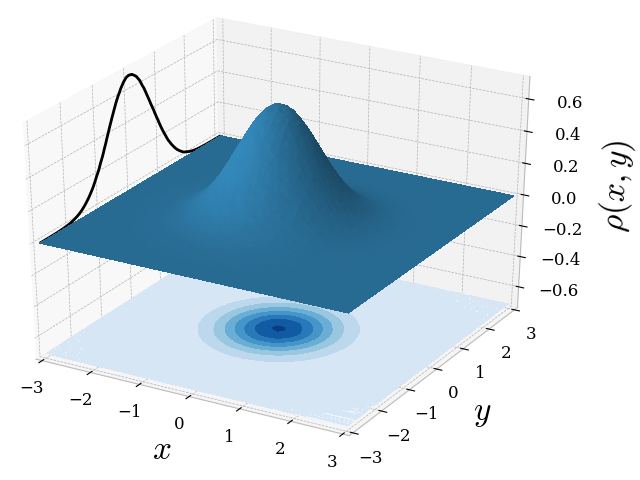
\includegraphics[width=5.1cm]{../plots/int0/onebody2/2D/2P/1.000000w/RBM_ADAM_MC268435456.png}}
	\subfloat{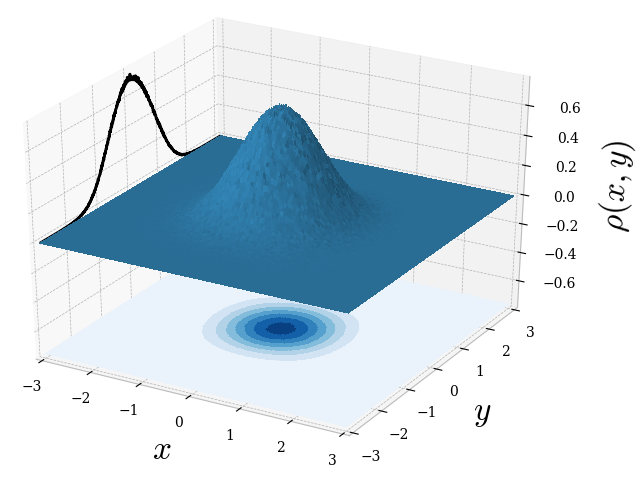
\includegraphics[width=5.1cm]{../plots/int0/onebody2/2D/2P/1.000000w/VMC_GD_MC2pow30_blue_small.png}}
	\subfloat{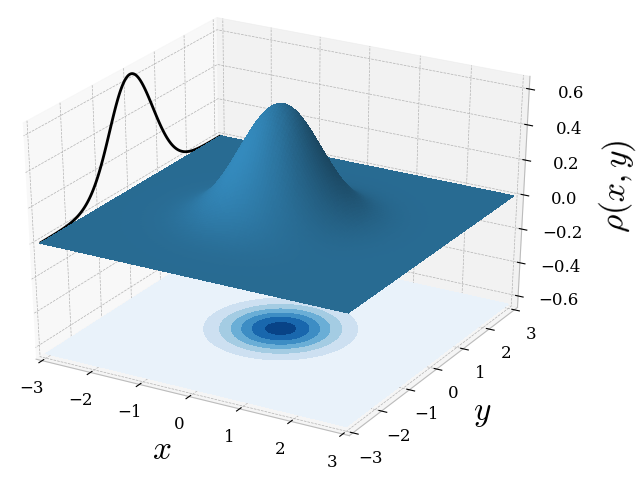
\includegraphics[width=5.1cm]{../plots/int0/onebody2/2D/2P/1.000000w/Exact.png}}
	
	\subfloat{\raisebox{2.cm}{\rotatebox[origin=t]{90}{Two-body}}}\hspace{0.1cm}
	\subfloat[RBM]{{
\includegraphics[width=5.1cm]{../plots/int0/twobody/RBM/2D/2P/1.000000w/RBM_GD_MC2pow30.png}}}
	\subfloat[VMC]{{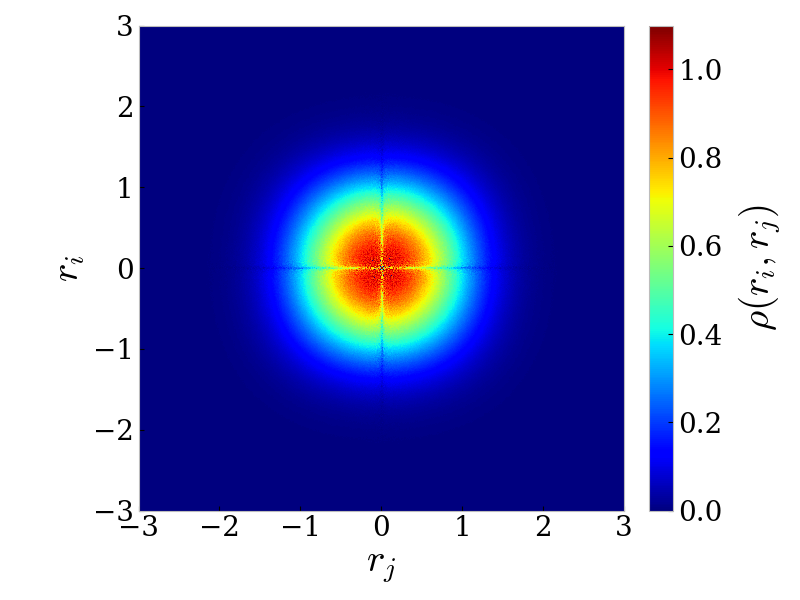
\includegraphics[width=5.1cm]{../plots/int0/twobody/VMC/2D/2P/1.000000w/VMC_GD_MC2pow30.png}}}
	\subfloat[Exact]{{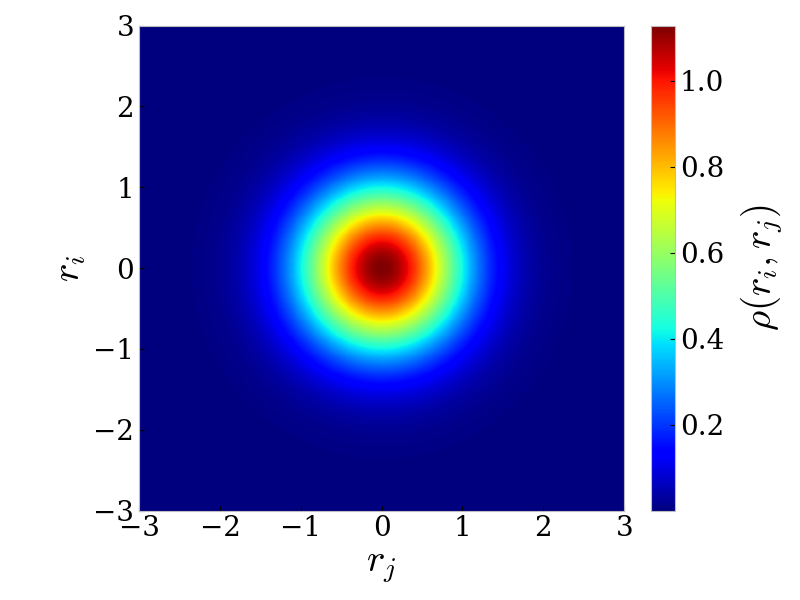
\includegraphics[width=5.1cm]{../plots/int0/twobody/VMC/2D/2P/1.000000w/exact.png}}}
	
	\caption{Electron density plots for a two-dimensional quantum dot with $N=2$ non-interacting electrons and frequency $\omega=1.0$ produces using RBM and VMC. The upper plots are the (spatial) one-body density distribution, where the surface plot and the contour plot on the $xy$-plane illustrate the density and the graph on the $yz$-plane represents the cross-section through $x=0$. The lower plots are the radial two-body density distributions. Besides, we compare the results to the exact densities, given by $\rho(x,y)\propto\exp(-x^2-y^2)$ and $\rho(r_i,r_j)\propto\exp(-r_i^2-r_j^2)$, respectively. For abbreviations see the text.}
	\label{fig:ED_nointeraction}
\end{figure}

As discussed before, the electron density should be normalized such that the integral over the density function $\rho$ corresponds to the number of particles $N$. For the one-body density, this corresponds to $\int dr\rho(r)=N$ for the radial density profile and $\int dxdy\rho(x,y)=N$ for the spatial density distribution and for the two-body radial density profile the normalization condition is $\int dr_idr_j\rho(r_i,r_j)=N$. However, there is no standard way of normalizing these densities when they are calculated using bins like us, as the normalization constant depends on the number of bins \textit{et cetera}. This is not very important either; we are only interested in the relative densities and the shapes of the density plots. We have been consequent when normalizing the density plots, such that the various density magnitudes can be compared to each other.

\iffalse
\newpage
\subsection{Double quantum dots}
For the double quantum dots, we can also find analytical energies without interaction, as explained in section \ref{sec:doubledots}. We first find the matrix 
\begin{equation*}
\hat{h}_{\nu\lambda}=\mel{\phi_{\nu}^{\text{HO}}(x)}{\hat{\mathcal{H}}_{\text{HO}}}{\phi_{\lambda}^{\text{HO}}(x)}+\mel{\phi_{\nu}^{\text{HO}}(x)}{\hat{\mathcal{H}}_{\text{+}}}{\phi_{\lambda}^{\text{HO}}(x)}
\end{equation*}
for a satisfying number of harmonic oscillator functions (basis functions). All the symbols are detailed in section \ref{sec:doubledots}. The energies are the eigenvalues of the matrix, which were obtained by the script \texttt{doublewell\_functions.py}. For one particle in one-dimensional potentials, we get the energy $E=0.3095$ for $\omega=1.0$ and $b=2$, and $E=0.1916$ for $\omega=0.5$ and $b=4$. This gives the analytical energies presented in table \eqref{tab:doubledotswointeraction}. 
\begin{table} [H]
	\caption{Energy of double quantum dots of frequency $\omega$ and with a splitting parameter $b$ containing two non-interacting electrons. The methods used were detailed in the introductory words of this chapter.}
	\label{tab:doubledotswointeraction}
	\begin{tabularx}{\textwidth}{lrrrR{3.5cm}R{3.5cm}R{3.5cm}} \hline\hline
		D & $\omega$ & $b$ & \makecell{\\ \phantom{=}} & RBM & VMC & Exact \\ \hline \\
		
		2D & 0.5 & 4.0 && - & - & 0.8832 \\
		& 1.0 & 2.0 && - & 1.6207(2) & 1.619 \\
		3D & 0.5 & 4.0 && - & - & 1.3832 \\
		& 1.0 & 2.0 && - & - & 2.619 \\ \hline\hline
	\end{tabularx}
\end{table}

The VMC reproduces the energies perfectly, while the RBM does not...
\fi

\newpage
\subsection{Atoms}
Lastly, we will look at atoms with non-interacting electrons in order to validate our code. The analytical energy of those atoms is given by the Bohr formula presented in equation \eqref{eq:bohrformula}. In table \eqref{tab:atomswointeraction}, the lowest closed-shell atoms Helium, Beryllium and Neon are listed with their exact energy and the obtained energy using VMC with hydrogen-like orbitals. Besides, we add calculations of the Hydrogen ground state energy as another simple test. What distinguish the implementation of atoms from the implementation of quantum dots, is that we are forced to include variational parameters in the Slater determinant for the atoms with atomic number $Z>2$. However, as all the energies are reproduced to machine-precision with the variational parameter $\alpha=1.0$, we have a clear indication that also this part works as it should.

\begin{table}[H]
	\caption{Energy of neutral atoms with atomic number $Z$ and non-interacting electrons. The energy is given in atomic units, see appendix \ref{app:units}. The variance is zero to machine-precision for all listed results. For abbreviations see the text.}
	\label{tab:atomswointeraction}
	\begin{tabularx}{\textwidth}{R{3.5cm}lrrR{2.5cm}R{2.5cm}} \hline\hline
		& Atom & $Z$ & \makecell{\\ \phantom{=}} & VMC & Exact \\ \hline \\
		
		& H & 1 && -0.5 & -0.5 \\
		& He & 2 && -4.0 & -4 \\
		& Be & 4 && -20.0 & -20 \\
		& Ne & 10 && -200.0 & -200 \\ \hline\hline
	\end{tabularx}
\end{table}

For completeness reasons, we also present the radial one-body density for Helium in figure \eqref{fig:helium_nointeraction}. The density is multiplied with $r^2$ in order to reveal the structure, and later in section \ref{sec:atomsresults} to compare the obtained density to other references. We see that the produced density curve is more or less identical to the exact density curve, found from the definition in section \ref{eq:electron_density}.

\begin{figure}[H]
	\centering
	\captionsetup[subfigure]{labelformat=empty}
	\subfloat{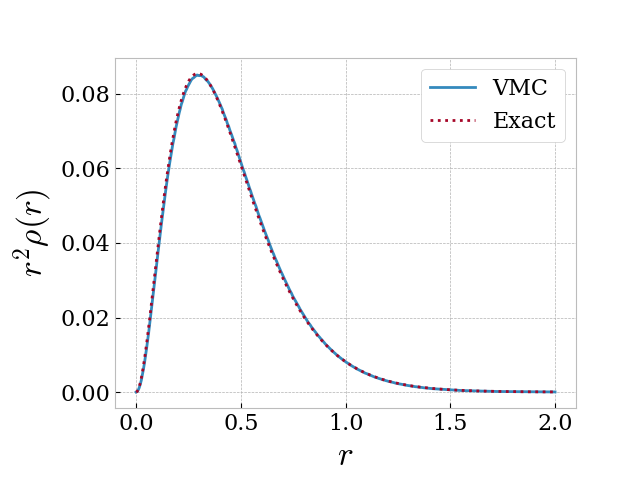
\includegraphics[width=9cm]{../plots/int0/onebody/helium.png}}
	\caption{Radial one-body density plot for the non-interacting Helium atom produced using VMC. The density was multiplied with $r^2$ in order to reveal the structures. For abbreviations see the text.}
	\label{fig:helium_nointeraction}
\end{figure}

\cleardoublepage
\section{Quantum dots} \label{sec:quantumdotresults}
We now move on to the more interesting case with repulsive interaction between the electrons. Analytical results are in general unavailable for this case, apart from a few semi-analytical energies and wave functions for the two- and three-dimensional quantum dots. We will for this system calculate the ground state energy, the one-body density, and the two-body density. 

The simulations are dependent on an array of parameters and factors, and in order to achieve good results, these hyper-parameters need to be reasonable. Firstly, the simulations are very sensitive about the learning rate, which needs to be small to avoid the quantum force to explode, but still large enough for the system to converge in an adequate number of iterations. Appropriate learning rates were found to be between $\eta=0.5$ and 0.00001 dependent on the system, where large systems and/or systems with low frequency required the lowest learning rates. Also, the step length needs to be specified cleverly, as we want to sample over the space where the particles physically can be located in a reasonable number of cycles. For a narrow oscillator potential (high frequency), the step length needs to be smaller than for a wide oscillator (low frequency). The acceptance ratio is directly dependent on the step length, where we want a high acceptance ratio to keep the computational cost low. However, we experienced that a too high acceptance ratio is neither favorable, as it can cause a very slow convergence or even a divergence. Also, the statistical error is largely dependent on the step length, and keeping an acceptance ratio at around 0.995 was found to be optimal, with a step length spanning from 0.01 to 1.0. The initial particle configurations and initial parameters are crucial to make the simulations converge rapidly. Lastly, the statistical error naturally also depends on the number of Monte Carlo cycles, where a high number of cycles is preferred as discussed in section \ref{sec:vmc}. We have applied an adaptive step number, which means that the number of cycles per iteration is increased for the last iterations. Firstly, this makes the final energy more accurate due to better statistics. Secondly, we get less noisy electron density plots by using this technique. All results below are produced using $2^{20}=1,048,576$ number of steps per iteration until the energy has converged. Then we run 10 more iterations with the number of steps increased to $2^{24}=16,777,216$ and for the very last iteration we run $2^{28}=268,435,456$ or $2^{30}=1,073,741,824$ steps.

Initially, we look at two-dimensional quantum dots with up to $N=56$ electrons and three-dimensional quantum dots with up to $N=40$ electrons and frequencies spanning from  $\omega=0.1$ to $\omega=1.0$. For those systems, we will compute the ground state energy, the one-body density, and the two-body density. After that, we move on to some special cases where the dots have low frequency ($\omega=0.01$) and large dots ($N>56$) to test how far we can go. For those systems, we will typically focus on either the ground state energy or the one-body density dependent on what we want to investigate. For instance, we will focus on the one-body density for low-frequency dots because of the search for Wigner localization. We also have a thorough discussion of how the energy is distributed between kinetic and potential energy, and compare this to the virial theorem.

\afterpage{
	\begin{landscape}
		\begin{table}
			\captionsetup{width=0.9\hsize}
			\caption{The ground state energy of two-dimensional circular quantum dots with frequency $\omega$ containing $N$ electrons. The HF results are taken from \citet{mariadason_quantum_2018}, the DMC results are taken from \citet{hogberget_quantum_2013} and semi-analytical results (Exact) are taken from \citet{taut_two_1994}. For abbreviations see the text. The energy is given in units of $\hbar$, and the numbers in parenthesis are the statistical uncertainties in the last digit.}
			\begin{tabularx}{\hsize}{llR{2.65cm}R{2.65cm}R{2.65cm}R{2.65cm}R{2.65cm}R{2.65cm}R{2.65cm}} \hline\hline
				\label{tab:quantumdotswinteraction2D1}
				\makecell{\\ $N$ \\ \phantom{=}} & $\omega$ & \multicolumn{1}{c}{RBM} & \multicolumn{1}{c}{RBM+SJ} & \multicolumn{1}{c}{RBM+PJ} & \multicolumn{1}{c}{\makecell{HF \\ (Ref.\cite{mariadason_quantum_2018})}} & \multicolumn{1}{c}{VMC} & \multicolumn{1}{c}{\makecell{DMC \\ (Ref.\cite{hogberget_quantum_2013})}} & \multicolumn{1}{c}{\makecell{Exact \\ (Ref.\cite{taut_two_1994})}} \\ \hline \\
				2 & 0.1 & 0.4728(1) & 0.44856(1) & 0.440975(8) & 0.525635 & 0.44129(1) & 0.44079(1) \\ 
				& 1/6 & 0.7036(1) & 0.67684(7) & 0.66715(6) & 0.768675 & 0.66710(1) & - & 2/3 \\
				& 0.28 & 1.07050(4) & 1.03470(7) & 1.021668(7) & 1.14171 & 1.02192(1) & 1.02164(1) \\
				& 0.5 & 1.72293(7) & 1.67739(9) & 1.659637(6) & 1.79974 & 1.65974(1) & 1.65977(1)  \\
				& 1.0 & 3.0803(2) & 3.02108(5) & 2.999587(5) & 3.16190 & 2.99936(1) & 3.00000(1) & 3.0 \\ 
				\hline \\
				
				6 & 0.1 & 3.697(1) & 3.63825(9) & 3.5700(2) & 3.85238 & 3.5695(1) & 3.55385(5) \\ 
				& 0.28 & 7.9273(9) & 7.7313(2) & 7.6203(2) & 8.01957 & 7.6219(1) & 7.60019(6) \\
				& 0.5 & 12.241(1) & 11.9659(5) & 11.8074(2) & 12.2713 & 11.8104(2) & 11.78484(6) \\
				& 1.0 & 20.716(1) & 20.3393(8) & 20.1832(2) & 20.7192 & 20.1918(2) & 20.15932(8) \\ \hline \\
				
				12 & 0.1 & 12.679(1) & 12.5964(7) & 12.3416(4) & 12.9247 & 12.29962(9) & 12.26984(8) \\ 
				& 0.28 & 26.389(2) & 26.051(1) & 25.7331(5) & 26.5500 & 25.7049(4) & 25.63577(9) \\
				& 0.5 & 40.440(3) & 39.6340(7) & 39.2743(6) & 40.2161 & 39.2421(5) & 39.1596(1) \\
				& 1.0 & 67.632(3) & 66.1898(8) & 65.7911(7) & 66.9113 & 65.7026(4) & 65.7001(1) \\ \hline
			\end{tabularx}
		\end{table}
		
		\begin{table}
			\label{tab:quantumdotswinteraction2D2}
			\begin{tabularx}{\hsize}{llR{2.65cm}R{2.65cm}R{2.65cm}R{2.65cm}R{2.65cm}R{2.65cm}R{2.65cm}} \\
				20 & 0.1 & 30.824(2) & 30.567(3) & 30.1553(9) & 31.1902 & 30.0403(2) & 29.9779(1) \\ 
				& 0.28 & 63.788(4) & 62.786(3) & 62.148(1) & 63.5390 & 62.0755(7) & 61.9268(1) \\
				& 0.5 & 96.410(1) & 94.920(4) & 94.104(1) & 95.7328 & 94.0433(9) & 93.8752(1) \\
				& 1.0 & 159.428(3) & 156.816(4) & 156.104(1) & 158.004 & 155.8900(4) & 155.8822(1) & \phantom{=} \\ 
				\hline \\
				
				30 & 0.1 & 61.829(5) & 61.198(2) & 60.774(2) & & 60.585(1) & 60.4205(2) \\ 
				& 0.28 & 126.958(6) & 125.413(2) & 124.437(2) & & 124.195(2) & 123.9683(2) \\
				& 0.5 & 191.495(7) & 188.995(5) & 187.488(2) & & 187.325(3) & 187.0426(2) \\
				& 1.0 & 315.364(8) & 309.997(6) & 308.989(2) & & 308.576(1) & 308.5627(2) \\ \hline \\
				
				42 & 0.1 & 109.892(6) & 109.48(2) & 108.183(1) & &  107.928(2) & 107.6389(2) \\ 
				& 0.28 & 224.462(8) & 224.184(9) & 222.200(5) & & 220.224(2) & 219.8426(2) \\
				& 0.5 & 337.523(8) & 333.582(9) & 331.410(3) & & 331.276(3) & 330.6306(2) \\
				& 1.0 & 553.40(1) & 545.817(9) & 543.746(3) & & 542.977(2) & 542.9428(8) \\ \hline \\
				
				56 & 0.1 & 179.789(6) & 179.59(1) & 178.501(5) & & 176.774(3) & 175.9553(7) \\ 
				& 0.28 & 364.85(1) & 364.165(9) & 359.83(2) & & 359.63(1) & 358.145(2) \\
				& 0.5 & 547.46(1) & 545.74(1) & 538.810(7) & & 538.686(9) & 537.353(2) \\
				& 1.0 & 894.12(2) & 882.93(1) & 881.010(5) & & 879.514(3) & 879.3986(6) \\ \hline\hline
			\end{tabularx}
		\end{table}
		
		\begin{table}
			\captionsetup{width=0.9\hsize}
			\caption{The ground state energy of two-dimensional circular quantum dots with frequency $\omega$ containing $N$ electrons.  The HF results are taken from \citet{mariadason_quantum_2018}, the DMC results are taken from \citet{hogberget_quantum_2013} and semi-analytical results (Exact) are taken from \citet{taut_two_1993}. For abbreviations see the text. The energy is given in units of $\hbar$, and the numbers in parenthesis are the statistical uncertainties in the last digit.} 
			\begin{tabularx}{\hsize}{llR{2.65cm}R{2.65cm}R{2.65cm}R{2.65cm}R{2.65cm}R{2.65cm}R{2.65cm}} \hline\hline
				\label{tab:quantumdotswinteraction3D1}
				\makecell{\\ $N$ \\ \phantom{=}} & $\omega$ & \multicolumn{1}{c}{RBM} & \multicolumn{1}{c}{RBM+SJ} & \multicolumn{1}{c}{RBM+PJ} & \multicolumn{1}{c}{\makecell{HF \\ (Ref.\cite{mariadason_quantum_2018})}} & \multicolumn{1}{c}{VMC} & \multicolumn{1}{c}{\makecell{DMC \\ (Ref.\cite{hogberget_quantum_2013})}} & \multicolumn{1}{c}{\makecell{Exact \\ (Ref.\cite{taut_two_1993})}} \\ \hline \\
				2 & 0.1 & 0.5177(1) & 0.50214(3) & 0.500080(6) & 0.529065 & 0.500083(7) & 0.499997(3) & 0.5 \\
				& 0.28 & 1.2261(1) & 1.20475(4) & 1.201710(6) & 1.23722 & 1.201752(6) & 1.201725(2) \\
				& 0.5 & 2.0269(1) & 2.00371(4) & 1.999912(5) & 2.03851 & 1.999977(5) & 2.000000(2) & 2.0 \\
				& 1.0 & 3.7574(1) & 3.73543(4) & 3.729827(5) & 3.77157 & 3.730030(5) & 3.730123(3) \\ 
				\hline \\
				
				8 & 0.1 & 5.8910(6) & 5.7498(4) & 5.718(4) & 5.86255 & 5.7126(1) & 5.7028(1) \\ 
				& 0.28 & 12.650(1) & 12.2492(4) & 12.2056(2) & 12.3987 & 12.2050(2) & 12.1927(1) \\
				& 0.5 & 19.487(2) & 19.0241(4) & 18.9747(2) & 19.1916 & 18.9759(1) & 18.9611(1) \\
				& 1.0 & 33.302(1) & 32.7159(6) & 32.6820(2) & 32.9246 & 32.6863(2) & 32.6680(1) \\ 
				\hline \\
				
				20 & 0.1 & 27.813(2) & 27.470(1) & 27.3382(8) & & 27.3144(5) & 27.2717(2) \\ 
				& 0.28 & 57.700(4) & 56.600(1) & 56.4477(6) & & 56.4297(5) & 56.3868(2) \\
				& 0.5 & 87.840(4) & 85.893(1) & 85.7153(6) & & 85.7161(5) & 85.6555(2) \\
				& 1.0 & 146.292(4) & 143.209(2) & 142.9409(6) & & 142.9560(7) & 142.8875(2) \\ \hline \\
				
				40 & 0.1 & 89.45(8) & 89.618(4) & 88.596(4) & & 88.182(1) \\ 
				& 0.28 & 182.714(6) & 181.877(4) & 179.630(1) & & 179.567(1) \\
				& 0.5 & 275.262(7) & 271.030(4) & 269.782(2) & & 269.746(1) \\
				& 1.0 & 452.732(8) & 442.874(4) & 442.630(1) & & 442.602(2) \\ \hline\hline
			\end{tabularx}
		\end{table}
	\end{landscape}
}

\subsection{Ground state energy} \label{sec:groundstateenergy}
The ground state energy is a natural starting point as our methods govern the minimization of the energy and it easily can be compared to benchmarks. By exploiting the symmetry of quantum dots with $n=2$ electrons, \citeauthor{taut_two_1993} was able to obtain semi-analytical energies for some specific frequencies $\omega$. More specifically, he found the energy to be $E=3$ for the frequency $\omega=1$ and $E=2/3$ for the frequency $\omega=1/6$ for the two-dimensional case \cite{taut_two_1993}, and $E=2$ for the frequency $\omega=1/2$ and $E=1/2$ for the frequency $\omega=1/10$ for the three-dimensional case \cite{taut_two_1994}. For other references, we need to rely on what researchers have found before us. Since diffusion Monte Carlo (DMC) is known to give very accurate results, we will mainly compare our results to the DMC computations of \citet{hogberget_quantum_2013}, which exist for quantum dots with up to $N=56$ electrons in two dimensions and with up to $N=20$ electrons in three dimensions. Comparing the energy to the Hartree-Fock (HF) limit is also interesting as the HF method approximates the electron-electron interactions by a mean-field, while the RBM needs to model the interactions itself. Practically, the RBM should give a lower energy than the HF method as the latter traditionally is notably computationally cheaper. We use the HF computations of \citet{mariadason_quantum_2018} for two-dimensional quantum dots with up to $N=20$ electrons and three-dimensional quantum dots with up to $N=8$ electrons. Computations for larger dots were not included, as they seem to not have converged.

Ground state energy computations of two- and three dimensional quantum dots are found in tables \eqref{tab:quantumdotswinteraction2D1} and \eqref{tab:quantumdotswinteraction3D1} respectively. They are computed by an RBM, RBM+SJ, RBM+PJ, and VMC, in addition to the HF limit and DMC that are present for reference purposes. The exact values are found in the last column with the same name. We observe that the method where less physical intuition is used, RBM, is the one that gives the highest energies among our implemented methods. This is as expected as no Jastrow factor is added to account for the correlations. For small quantum dots ($N<8$), the RBM energy is lower than the HF limit, and for low frequencies ($\omega<0.5$) the RBM energy is generally also lower. However, for higher frequencies and larger dots, the HF limit is lower than the energy obtained with the RBMs. It is apparent that the mean-field approximation works better than the RBM when the interactions get less important. When we add more intuition in the form of a simple Jastrow factor, the energy drops significantly, especially for high frequencies. It is, therefore, lower than the HF limit for all simulations, and surprisingly close to the reference considering the simple form of the Jastrow factor. The statistical errors of the RBM+SJ is in general smaller than for RBM, which is a good indication that the method provides a better ground state estimate as the actual ground state obeys a zero-variance property. 

Furthermore, we added a more complex Jastrow factor in the form of a Padé-Jastrow factor, and we observe that the energy drops further. The RBM+PJ provides energies entirely on par with VMC, in many cases even lower. Notably, RBM+PJ provides the lowest energies among our implemented methods for dots with two electrons, and the statistical errors are also the lowest. This hints that RBM+PJ can obtain a better ground state estimate than VMC for the smallest dots, which makes sense as the former method is more flexible than VMC. However, for large dots, RBM+PJ provides slightly higher energies than VMC, which we suspect is a result of the large number of variational parameters, and thus a too complex model for the problem. If we recall that the number of hidden units is set to the number of electrons, the number of variational parameters increases rapidly as the number of electrons increases. To see if the problem occurs because the model has not converged, we have decreased the number of hidden nodes for some selected systems, and it has given promising results.

We also see that all the methods can obtain energies closer to the reference energy in three dimensions compared to two dimensions. This is a well-known concept and occurs because we have more degrees of freedom. One can imagine that the electrons can move in the space instead of just on a plane, which makes it easier to form a configuration that minimizes the energy. 

Efforts were made to reproduce the results using a partly restricted Boltzmann machine and a deep belief network, but due to convergence problems and energy fluctuations, the methods were not investigated further. 

\begin{figure}
	\centering
	\captionsetup[subfigure]{labelformat=empty}
	\subfloat{\raisebox{2.5cm}{\rotatebox[origin=t]{90}{$N=2$}}}\hspace{0.1cm}
	\subfloat{{\includegraphics[width=7.8cm]{../plots/int1/onebody2/2D/2P/1.000000w/RBM_ADAM_MC2pow28_smooth_blue.png}}}\hspace{-0.0cm}
	\subfloat{{\includegraphics[width=7.8cm]{../plots/int1/onebody2/2D/2P/1.000000w/VMC_ADAM_MC2pow28_smooth_blue.png}}}\\
	
	\subfloat{\raisebox{2.5cm}{\rotatebox[origin=t]{90}{$N=6$}}}\hspace{0.05cm}
	\subfloat{{\includegraphics[width=7.8cm]{../plots/int1/onebody2/2D/6P/1.000000w/RBM_ADAM_MC2pow28_smooth_blue.png}}}\hspace{-0.0cm}
	\subfloat{{\includegraphics[width=7.8cm]{../plots/int1/onebody2/2D/6P/1.000000w/VMC_ADAM_MC2pow28_smooth_blue.png}}}\\
	
	\subfloat{\raisebox{2.5cm}{\rotatebox[origin=t]{90}{$N=12$}}}\hspace{0.1cm}
	\subfloat[RBM]{{\includegraphics[width=7.8cm]{../plots/int1/onebody2/2D/12P/1.000000w/RBM_ADAM_MC2pow28_smooth_blue.png}}}\hspace{-0.0cm}
	\subfloat[VMC]{{\includegraphics[width=7.8cm]{../plots/int1/onebody2/2D/12P/1.000000w/VMC_ADAM_MC2pow28_smooth_blue.png}}}
	
	\caption{One-body density plots for two-dimensional quantum dots with frequency $\omega=1.0$, where the surface plot and the contour plot on the $xy$-plane illustrate the density and the graph on the $yz$-plane represents the cross-section through $x=0$. From the top, the plots present quantum dots with $N=2$, 6 and 12 electrons, and were all obtained using RBM (right column) and VMC (left column). The ADAM optimizer was used, and after convergence the number of Monte Carlo cycles was $M=2^{30}=1,073,741,824$. The plots are noise-reduced using a Savitzky-Golay filter, and for abbreviations see the text.}
	\label{fig:OB_interaction_1p0w1}
\end{figure}
\begin{figure}
	\centering
	\captionsetup[subfigure]{labelformat=empty}
	\subfloat{\raisebox{2.5cm}{\rotatebox[origin=t]{90}{$N=20$}}}\hspace{0.1cm}
	\subfloat{{\includegraphics[width=7.8cm]{../plots/int1/onebody2/2D/20P/1.000000w/RBM_ADAM_MC2pow28_smooth_blue.png}}}\hspace{-0.0cm}
	\subfloat{{\includegraphics[width=7.8cm]{../plots/int1/onebody2/2D/20P/1.000000w/VMC_ADAM_MC2pow28_smooth_blue.png}}}\\
	
	\subfloat{\raisebox{2.5cm}{\rotatebox[origin=t]{90}{$N=30$}}}\hspace{0.1cm}
	\subfloat{{\includegraphics[width=7.8cm]{../plots/int1/onebody2/2D/30P/1.000000w/RBM_ADAM_MC2pow28_smooth_blue.png}}}\hspace{-0.0cm}
	\subfloat{{\includegraphics[width=7.8cm]{../plots/int1/onebody2/2D/30P/1.000000w/VMC_ADAM_MC2pow28_smooth_blue.png}}}\\
	
	\subfloat{\raisebox{2.5cm}{\rotatebox[origin=t]{90}{$N=42$}}}\hspace{0.1cm}
	\subfloat[RBM]{{\includegraphics[width=7.8cm]{../plots/int1/onebody2/2D/42P/1.000000w/RBM_ADAM_MC2pow28_smooth_blue.png}}}\hspace{-0.0cm}
	\subfloat[VMC]{{\includegraphics[width=7.8cm]{../plots/int1/onebody2/2D/42P/1.000000w/VMC_ADAM_MC2pow28_smooth_blue.png}}}
	
	\caption{One-body density plots for two-dimensional quantum dots with frequency $\omega=1.0$, where the surface plot and the contour plot on the $xy$-plane illustrate the density and the graph on the $yz$-plane represents the cross-section through $x=0$. From the top, the plots present quantum dots with $N=20$, 30 and 42 electrons, and were all obtained using RBM (right column) and VMC (left column). The ADAM optimizer was used, and after convergence the number of Monte Carlo cycles was $M=2^{30}=1,073,741,824$. The plots are noise-reduced using a Savitzky-Golay filter, and for abbreviations see the text.}
	\label{fig:OB_interaction_1p0w2}
\end{figure}

\subsection{One-body density} \label{sec:onebodyresults}
Another quantity of particular interest is the one-body density. For all the systems presented in tables \eqref{tab:quantumdotswinteraction2D1} and \eqref{tab:quantumdotswinteraction3D1} we have also calculated the one-body density. However, since all of those plots would occupy tens of pages, we will not present all of them here. Instead, we select a few sample plots that might be interesting for the reader and give a representative picture of the density. The total collection of one-body density plots can be found in section \ref{sec:onebody} in appendix \ref{chp:totalresults}. 

We have computed the one-body density in two different ways: by dividing the space into annuluses and obtaining the radial density profile, as discussed in section \ref{sec:electrondensityimplementation}, and by dividing the space into a grid of equally sized bins and obtaining the density profile throughout the space. The former is computationally beneficial as the density typically is stored in $n$ bins compared to $n^2$ bins for the second method, but the latter is clearly able to store more information. The second method is thereby able to give more informative plots, but when we want to compare the various methods, a radial density profile is more convenient. In other words, there are pros and cons associated with both methods, and we will, therefore, present both to give an as comprehensive description of the results as possible. 

Initially, we will present the spatial density profiles for two-dimensional quantum dots of frequency $\omega=1.0$. In figure \eqref{fig:OB_interaction_1p0w1} and \eqref{fig:OB_interaction_1p0w2}, the evolution of the one-body density for dots of sizes $N=2$, 6, 12, 20, 30 and 42 are presented, produced with RBM and VMC. To maximize the amount of information in the plots, we have included a graph presenting the cross-section through $x=0$ on the $yz$-plane and a contour plot of the density on the $xy$-plane, in addition to a 3D surface plot of the density. What we observe is that the density profile is smooth, with more peaks as the number of particles increases, representing high densities. For an odd number of shells ($N=2$, 12 and 30) the density has its maximum at the center of the dot, resulting in equal shapes where for example the shape of $N=12$ is seen as the top of $N=30$. On the other hand, for an even number of shells ($N=6$, 20 and 42) the highest density is found at a ridge that encircles the center, and also here the shape of for example $N=20$ is seen as the top of $N=42$. It is apparent that those are the configurations that minimize the energy, with a structure following directly from the Pauli principle, as the electrons are forced to distribute over multiple shells. Even when we remove the interaction between the electrons, we get the same characteristic wave shape, though narrower. The RBM provides sharper and more distinct peaks than the VMC, but at least the extrema seem to be located at the same radii. These differences are caused by the ways the methods model the correlations, where the VMC employs the Padé-Jastrow factor, and the RBM needs to find the best way to account for the correlations itself. To connect the observations to something everyone is familiar with, we can compare the density plots to water ripples if one sees it from the smallest to the largest dot. \citet{hogberget_quantum_2013} discusses this in his master thesis, and his one-body densities are consistent with what we have obtained. However, for $N=42$ the RBM provides a density profile that has ripples in both radial and angular direction, indicating that the simulation has not fully converged to the minimum. This might be an effect of the large number of variational parameters. One-body density plots for the same systems using an RBM+SJ and RBM+PJ were generated, but in order to limit us to a few plots we decided to keep the extremes here, and placed the others in appendix \ref{chp:totalresults}.

In figure \eqref{fig:OB_interaction_23D}, we stick to frequency $\omega=1.0$ for small two- and three-dimensional quantum dots and compare the results obtained by VMC, RBM, RBM+SJ, and RBM+PJ. We investigate dots with $N=2$, 6 and 12 in two dimensions and $N=2$, 8 and 20 in three dimensions, which corresponds to one shell ($S=1$), two shells ($S=2$) and three shells ($S=3$), respectively. For all the numbers of shells, we immediately see that the density plots are identical for two- and three-dimensional dots. The same phenomenon was observed for quantum dots with non-interacting electrons in figure \eqref{fig:OB_nointeraction}, which can easily be explained as the wave function is trivially separable. However, this is not the situation when we look at the interacting case, and it was therefore not obvious to us that the same phenomenon would occur here. Physically, this means that the electrons configure in the same way in three dimensions as in two dimensions, 
\begin{figure}[H]
	\centering
	\captionsetup[subfigure]{labelformat=empty}
	\subfloat{\raisebox{1.5cm}{\rotatebox[origin=t]{90}{$S=1$}}}\hspace{0.1cm}
	\subfloat{{\includegraphics[width=5.1cm]{../plots/int1/onebody2/2D/2P/1.000000w/VMC_ADAM_MC2pow28_smooth_blue_small.png}}}\hspace{-0.0cm}
	\subfloat{{\includegraphics[width=5.1cm]{../plots/int1/onebody/2D/2P/1.000000w/ADAM_MC1048576.png}}}\hspace{-0.5cm}
	\subfloat{{\includegraphics[width=5.1cm]{../plots/int1/onebody/3D/2P/1.000000w/ADAM_MC1048576.png}}}\\ [-0.2cm]
	
	\subfloat{\raisebox{1.5cm}{\rotatebox[origin=t]{90}{$S=2$}}}\hspace{0.1cm}
	\subfloat{{\includegraphics[width=5.1cm]{../plots/int1/onebody2/2D/6P/1.000000w/VMC_ADAM_MC2pow28_smooth_blue_small.png}}}\hspace{-0.0cm}
	\subfloat{{\includegraphics[width=5.1cm]{../plots/int1/onebody/2D/6P/1.000000w/ADAM_MC1048576.png}}}\hspace{-0.5cm}
	\subfloat{{\includegraphics[width=5.1cm]{../plots/int1/onebody/3D/8P/1.000000w/ADAM_MC1048576.png}}}\\ [-0.2cm]
	
	\subfloat{\raisebox{1.5cm}{\rotatebox[origin=t]{90}{$S=3$}}}\hspace{0.1cm}
	\subfloat[VMC, 2D]{{\includegraphics[width=5.1cm]{../plots/int1/onebody2/2D/12P/1.000000w/VMC_ADAM_MC2pow28_smooth_blue_small.png}}}\hspace{-0.0cm}
	\subfloat[2D]{{\includegraphics[width=5.1cm]{../plots/int1/onebody/2D/12P/1.000000w/ADAM_MC1048576.png}}}\hspace{-0.5cm}
	\subfloat[3D]{{\includegraphics[width=5.1cm]{../plots/int1/onebody/3D/20P/1.000000w/ADAM_MC1048576.png}}}
	
	\caption{One-body density plot for small quantum dots with frequency $\omega=1.0$. We look at the three lowest shells $S=1$, 2 and 3 corresponding to $N=2$, 6, and 12 electrons in two dimensions and $N=2$, 8 and 20 electrons in three dimensions. In the first column, the surface plot and the contour plot on the $xy$-plane illustrate the density and the graph on the $yz$-plane represents the cross-section through $x=0$. In the middle column, the corresponding radial density profiles are obtained using RBM, RBM+SJ, RBM+PJ and VMC. On the right-hand side, the radial density profiles for the three-dimensional dots are given using the same methods. ADAM optimizer was used, and after convergence, the number of Monte-Carlo cycles was $M=2^{30}=1,073,741,824$. The surface plots are noise-reduced using a Savitzky-Golay filter, and for abbreviations see the text.}
	\label{fig:OB_interaction_23D}
\end{figure}
\noindent
where the average distance from a "shell" to the center of the dot is dimensionless. Besides the physics, we are also interested in analyzing the performance of the various methods. We observe that all the methods give quite similar radial density profiles, but RBM is always the guy standing out. Apparently, the RBM tends to exaggerate the peaks discussed above and gives an even more wavy density plot, as also observed in figures \eqref{fig:OB_interaction_1p0w1} and \eqref{fig:OB_interaction_1p0w2}. Further, the RBM+SJ is more similar to the VMC and RBM+PJ, which are almost identical. This is consistent with the energy analysis in section \ref{sec:groundstateenergy}, where we found VMC and RBM+PJ to be the most accurate methods, followed by RBM+SJ and RBM. We also observe some noise close to $r=0$, which is caused by the fact that the number of Monte Carlo cycles is finite and we in practice have bins of different sizes.

\begin{figure}
	\centering
	\captionsetup[subfigure]{labelformat=empty}
	\subfloat{\raisebox{3cm}{\rotatebox[origin=t]{90}{$\omega=0.1$}}}\hspace{0.1cm}
	\subfloat{{\includegraphics[width=8cm]{../plots/int1/onebody/2D/20P/0.100000w/ADAM_MC1048576.png}}}\hspace{-0.5cm}
	\subfloat{{\includegraphics[width=8cm]{../plots/int1/onebody/2D/42P/0.100000w/ADAM_MC1048576.png}}}\\
	
	\subfloat{\raisebox{3cm}{\rotatebox[origin=t]{90}{$\omega=0.5$}}}\hspace{0.1cm}
	\subfloat{{\includegraphics[width=8cm]{../plots/int1/onebody/2D/20P/0.500000w/ADAM_MC1048576.png}}}\hspace{-0.5cm}
	\subfloat{{\includegraphics[width=8cm]{../plots/int1/onebody/2D/42P/0.500000w/ADAM_MC1048576.png}}}\\
	
	\subfloat{\raisebox{3cm}{\rotatebox[origin=t]{90}{$\omega=1.0$}}}\hspace{0.1cm}
	\subfloat[20P]{{\includegraphics[width=8cm]{../plots/int1/onebody/2D/20P/1.000000w/ADAM_MC1048576.png}}}\hspace{-0.5cm}
	\subfloat[42P]{{\includegraphics[width=8cm]{../plots/int1/onebody/2D/42P/1.000000w/ADAM_MC1048576.png}}}
	
	\caption{One-body density plot for two-dimensional quantum dots with oscillator frequencies $\omega=0.1$, 0.5 and 1.0 and $N=20$, 42 electrons. The ADAM optimizer was used, and after convergence the number of Monte-Carlo cycles was $M=2^{28}=268,435,456$. For abbreviations see the text.}
	\label{fig:OB_interaction}
\end{figure}

We now move on to larger two-dimensional dots and lower frequencies than $\omega=1.0$ to see if the physics is conserved also when the interactions get stronger. In figure \eqref{fig:OB_interaction}, we plot the radial density profile for two-dimensional quantum dots with $N=20,42$ and frequencies $\omega=0.1$, 0.5 and 1.0 to compare all the methods again. What we see is that the peaks discussed above are conserved for lower frequencies, and they change slightly as the frequency drops. Also, the density distribution is spatially expanded as the frequency drops, since the force pushing the electrons towards the center of the dot gets weaker. All the methods VMC, RBM+PJ, and RBM+SJ appear to give quite similar density plots, but for lower frequencies, the difference gets gradually more visible. In particular, the peaks for frequency $\omega=0.1$ do no longer match for the various methods. Especially RBM and RBM+SJ differ from VMC and RBM+PJ, which is again a clear indication that the final results are heavily dependent on the way the methods account for the correlations. RBM+SJ tends to slightly exaggerate the peaks in the density plots, and RBM takes the exaggeration to the next level. This trend was also observed in the plots in figures (\ref{fig:OB_interaction_1p0w1}, \ref{fig:OB_interaction_1p0w2}, \ref{fig:OB_interaction_23D}), and technically speaking, this means that the method is capable of finding the most likely places to find the electrons, but fails to determine the actual density there. We have also seen that the one-body density is shape-invariant for the frequencies $\omega=0.5$ and 1.0 except for their radial extent. For that reason, it is not very exciting to further study those high frequencies, and in section \ref{sec:lowfrequencies} we move on to low-frequency dots.

\subsection{Two-body density}
We have on multiple occasions in this thesis discussed the electron density, and we have also mentioned the two-body density. The two-body density gives the probability of finding an electron at a certain position, given the position of another electron. Unlike the one-body density, this density, therefore, gives the information of how the particles distribute pairwise, and it is therefore very informative when we want to study the electron-electron correlations. Similarly to the one-body density, we can both plot the radial two-body density profile and the actual two-body density distribution throughout the space. However, since the latter results in a higher-dimensional object, we stick to the radial density profile. Also for this quantity, it would be convenient to have references to benchmark our results, but for some reason, it is hard to find papers that discuss the two-body density for quantum dots. Nevertheless, someone needs to be the first, and we will use the plots to discuss physics and compare the various methods in the best possible way. Again, we will emphasize that a negative radial distance does not make sense, so all the quadrants in the two-body density plots are the same and presented in this way to make them more illustrative and intuitive. We will focus on the two-dimensional case, as the three-dimensional case becomes similar in the same way as for the one-body density. 

In figure \eqref{fig:TB_interaction_2P}, we plot the two-body density for a two-dimensional quantum dot with $N=2$ and frequencies $\omega=0.1$, 0.5 and 1.0. For the frequency $\omega=1.0$, the density plots for all the methods give quite similar results, but the RBM provides a higher two-body density in the middle of the quantum dot, compared to the other methods. This can be seen from the magnitude of the density at the center, but also the density itself is narrower than for its fellow methods, making it more compact. This can be explained by the absence of a Jastrow factor. Also, the RBM+SJ gives a slightly narrower distribution than the RBM+PJ and VMC, so it is apparent that the Padé-Jastrow factor results in a more repulsive factor than the simple Jastrow factor. The same indication can be seen at the density at the origin, which is low for RBM+PJ and VMC, but high for RBM and RBM+SJ. Furthermore, we know that the potential, and thus the interactions, get more dominating as the frequency drops. For VMC and RBM+PJ, this can be observed by a significant circle of higher density at a certain distance from the origin both for $\omega=0.5$ and $\omega=0.1$, which physically means that both particles are less likely to be found in the center of the dot at the same time. If one particle is close to the center, the other particle is probably far from the center and \textit{vice versa}. For the RBM+SJ, this behavior can only be observed 

\begin{landscape}
	\begin{figure}
		\centering
		\captionsetup{width=0.9\hsize}
		\captionsetup[subfigure]{labelformat=empty}
		\subfloat{\raisebox{2cm}{\rotatebox[origin=t]{90}{$\omega=0.1$}}}\hspace{0.1cm}
		\subfloat{{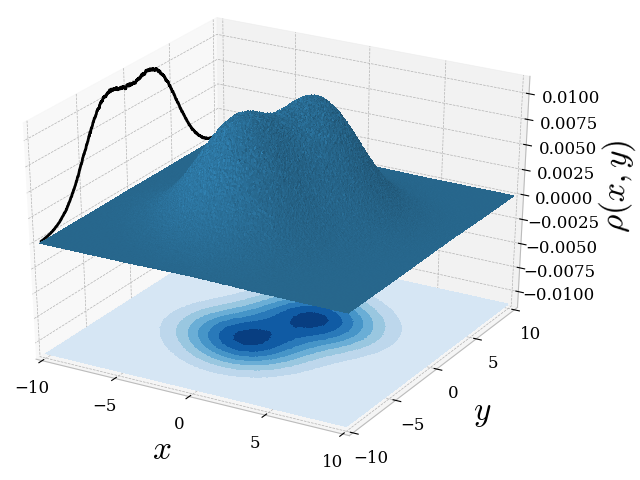
\includegraphics[width=5.7cm]{../plots/int1/twobody/2D/2P/0.100000w/RBM_ADAM_MC1048576.png}}}
		\subfloat{{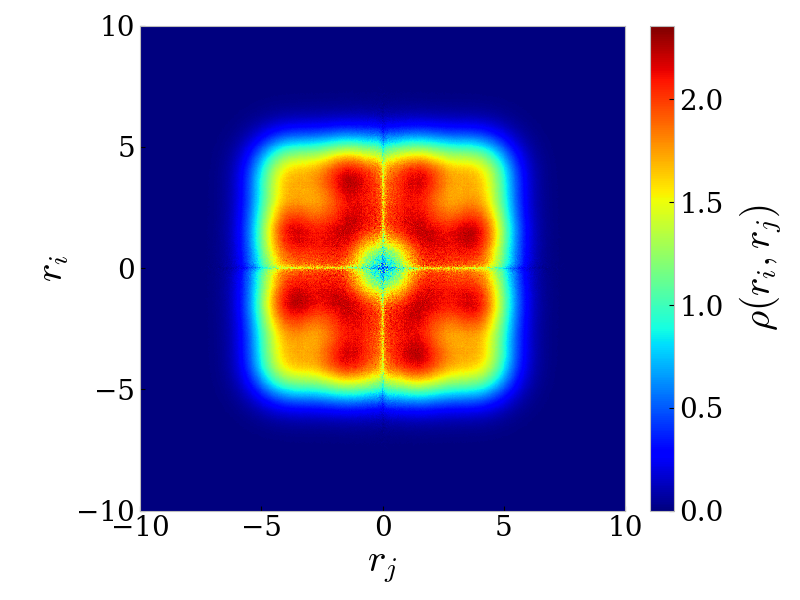
\includegraphics[width=5.7cm]{../plots/int1/twobody/2D/2P/0.100000w/RBMSJ_ADAM_MC1048576.png}}}
		\subfloat{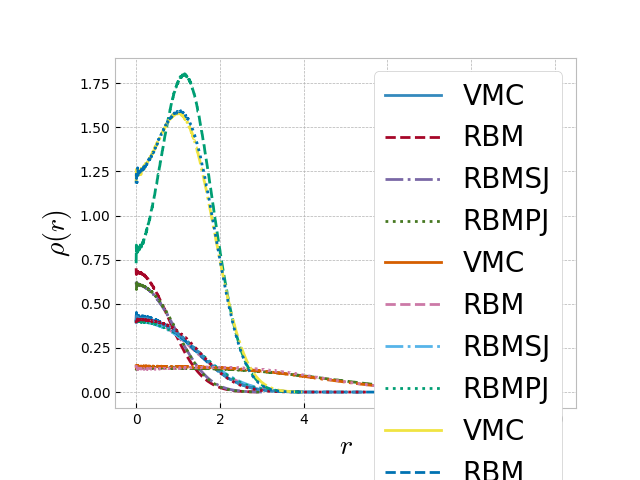
\includegraphics[width=5.7cm]{../plots/int1/twobody/2D/2P/0.100000w/RBMPJ_ADAM_MC1048576.png}}
		\subfloat{{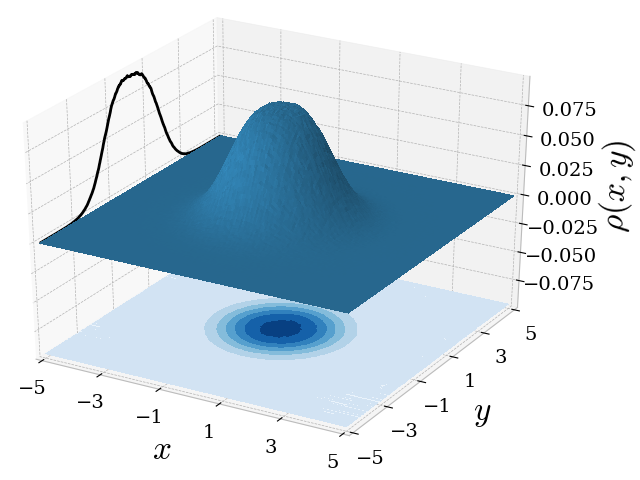
\includegraphics[width=5.7cm]{../plots/int1/twobody/2D/2P/0.100000w/VMC_ADAM_MC1048576.png}}}
		
		\subfloat{\raisebox{2cm}{\rotatebox[origin=t]{90}{$\omega=0.5$}}}\hspace{0.1cm}
		\subfloat{{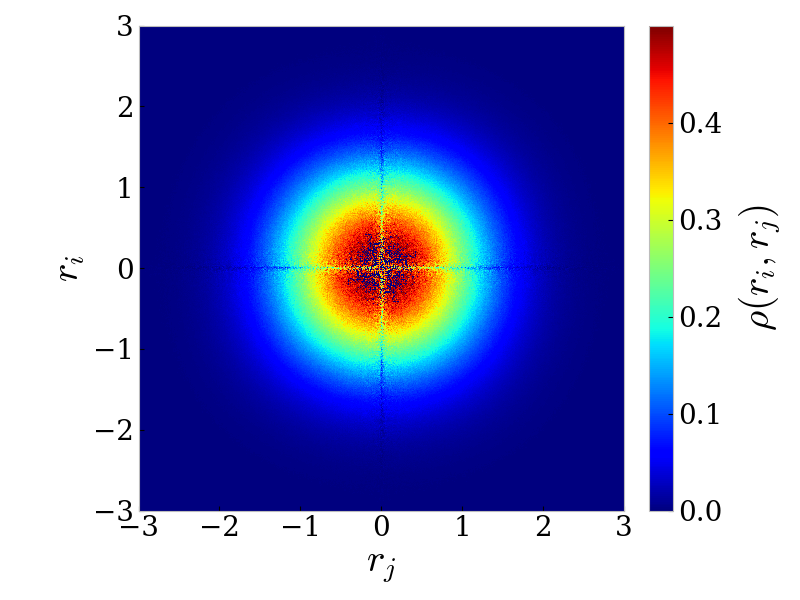
\includegraphics[width=5.7cm]{../plots/int1/twobody/2D/2P/0.500000w/RBM_ADAM_MC1048576_zoomed.png}}}
		\subfloat{{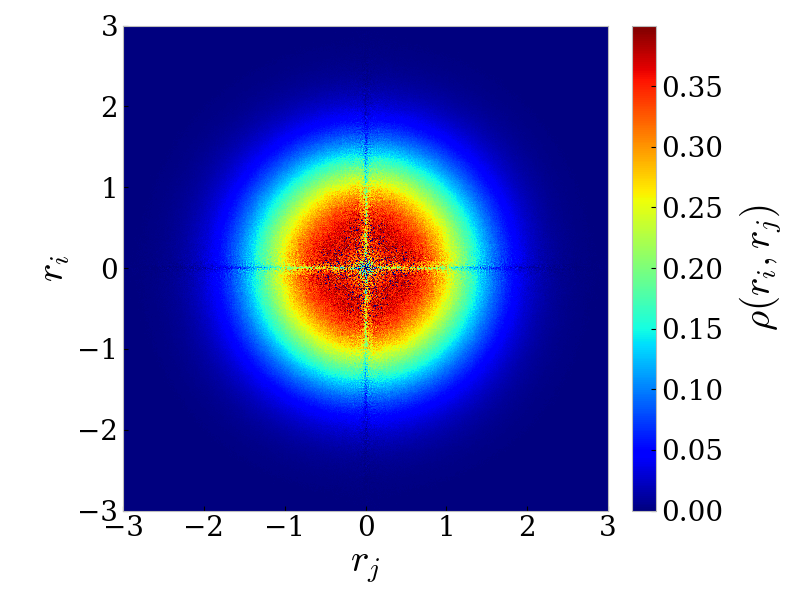
\includegraphics[width=5.7cm]{../plots/int1/twobody/2D/2P/0.500000w/RBMSJ_ADAM_MC1048576_zoomed.png}}}
		\subfloat{\includegraphics[width=5.7cm]{../plots/int1/twobody/2D/2P/0.500000w/RBMPJ_ADAM_MC1048576_zoomed.png}}
		\subfloat{{\includegraphics[width=5.7cm]{../plots/int1/twobody/2D/2P/0.500000w/VMC_ADAM_MC1048576_zoomed.png}}}\\
		
		\subfloat{\raisebox{2cm}{\rotatebox[origin=t]{90}{$\omega=1.0$}}}\hspace{0.1cm}
		\subfloat[RBM]{{\includegraphics[width=5.7cm]{../plots/int1/twobody/2D/2P/1.000000w/RBM_ADAM_MC1048576_zoomed.png}}}
		\subfloat[RBM+SJ]{{\includegraphics[width=5.7cm]{../plots/int1/twobody/2D/2P/1.000000w/RBMSJ_ADAM_MC1048576_zoomed.png}}}
		\subfloat[RBM+PJ]{{\includegraphics[width=5.7cm]{../plots/int1/twobody/2D/2P/1.000000w/RBMPJ_ADAM_MC1048576_zoomed.png}}}
		\subfloat[VMC]{{\includegraphics[width=5.7cm]{../plots/int1/twobody/2D/2P/1.000000w/VMC_ADAM_MC1048576_zoomed.png}}}
		
		\caption{Two-body density plots for two-dimensional quantum dots with $N=2$ electrons and oscillator frequencies $\omega=0.1$, 0.5 and 1.0. The ADAM optimizer was used, and after convergence the number of Monte-Carlo cycles was $M=2^{28}=268,435,456$. For abbreviations see the text.}%
		\label{fig:TB_interaction_2P}
	\end{figure}
\end{landscape}
\begin{figure}[H]
	\centering
	\captionsetup{width=0.9\hsize}
	\captionsetup[subfigure]{labelformat=empty}
	\subfloat{\raisebox{2.5cm}{\rotatebox[origin=t]{90}{$N=6$}}}\hspace{0.1cm}
	\subfloat{{\includegraphics[width=7cm]{../plots/int1/twobody/2D/6P/0.500000w/RBM_ADAM_MC1048576.png}}}
	\subfloat{{\includegraphics[width=7cm]{../plots/int1/twobody/2D/6P/0.500000w/VMC_ADAM_MC1048576.png}}}\\
	
	\subfloat{\raisebox{2.5cm}{\rotatebox[origin=t]{90}{$N=20$}}}\hspace{0.1cm}
	\subfloat{{\includegraphics[width=7cm]{../plots/int1/twobody/2D/20P/0.500000w/RBM_ADAM_MC1048576.png}}}
	\subfloat{{\includegraphics[width=7cm]{../plots/int1/twobody/2D/20P/0.500000w/VMC_ADAM_MC1048576.png}}}\\
	
	\subfloat{\raisebox{2.5cm}{\rotatebox[origin=t]{90}{$N=42$}}}\hspace{0.1cm}
	\subfloat[RBM]{\includegraphics[width=7cm]{../plots/int1/twobody/2D/42P/0.500000w/RBM_ADAM_MC1048576.png}}
	\subfloat[VMC]{{\includegraphics[width=7cm]{../plots/int1/twobody/2D/42P/0.500000w/VMC_ADAM_MC1048576.png}}}
	
	\caption{Two-body density plots for two-dimensional quantum dots with an even number of closed shells ($N=6$, 20 and 42 electrons) and oscillator frequency $\omega=0.5$. The ADAM optimizer was used, and after convergence, the number of Monte-Carlo cycles was $M=2^{28}=268,435,456$. For abbreviations see the text.}%
	\label{fig:TB_interaction_20P}
\end{figure}
\noindent
for $\omega=0.1$, while the RBM is not able to reproduce this phenomenon at all. This indicates that the RBM is not able to model the correlations correctly, and it needs a Jastrow factor to account for them. The resolutions of the plots get lower when we decrease the frequency, as the particles spread over a larger area and therefore more bins.

The calculations are repeated for two-dimensional quantum dots with frequency $\omega=0.5$ and an even number of closed shells ($N=6$, 20 and 42), with radial two-body density plots presented in figure \eqref{fig:TB_interaction_20P}. The first thing we observe is that the RBM manages to obtain the correct peaks, but all the peaks are circular unlike the density plots from the VMC, and they are also more distinct and higher than for VMC. This is the same effect we saw in the one-body density plots, which we argued was caused by the different approaches to model the correlations. If we now keep our attention on the VMC plots, it is apparent that two particles will not be observed in the middle of the dot at the same time, as the density there is almost absent. For $N=6$, a particle pair is most likely to be found at the same radius around $r=2$, which matches the one-body density plot. When we move on to $N=20$, the most probable location is not ambiguous anymore, but an electron pair is likely to be found at the same radius at around $r=1$, which matches the highest peak in the one-body density plot. However, the density is also high along both axes, which means that if one of the electrons moves towards the center of the dot, the other will also move towards the center. This is probably a consequence of the repulsive interactions. For $N=42$, finding two electrons at the same radius is not the most likely case anymore. This is because the electrons now spread over a large area. The density plot clearly has some distinct peaks around $r_i\sim 2$ and $r_j\sim 1$, matching the peaks found in the one-body density plots. For dots with an odd number of closed shells, the same tendency was found, but the peaks were found at the intersection between the quadrants, again matching the one-body density. 

\iffalse
\begin{figure}[H]
	\centering 
	\captionsetup[subfigure]{labelformat=empty}
	\subfloat[RBM]{{% This file was created by tikzplotlib v0.8.1.
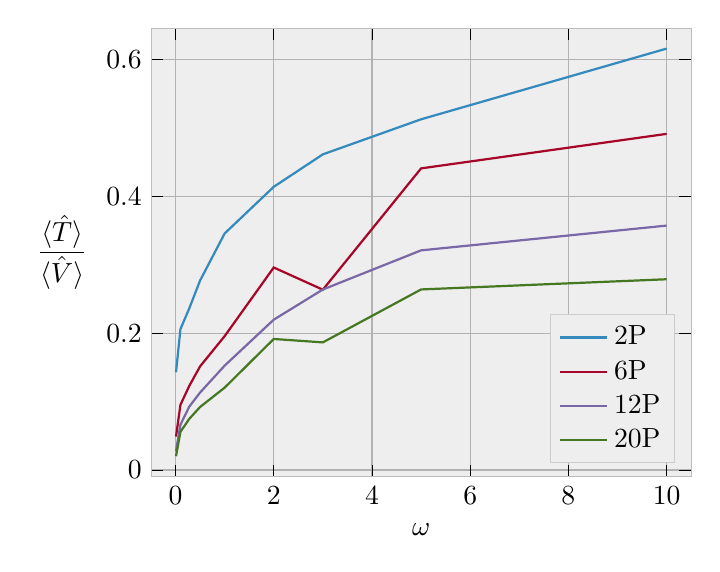
\begin{tikzpicture}

\definecolor{color0}{rgb}{0.203921568627451,0.541176470588235,0.741176470588235}
\definecolor{color1}{rgb}{0.650980392156863,0.0235294117647059,0.156862745098039}
\definecolor{color2}{rgb}{0.47843137254902,0.407843137254902,0.650980392156863}
\definecolor{color3}{rgb}{0.274509803921569,0.470588235294118,0.129411764705882}

\begin{axis}[
axis background/.style={fill=white!93.33333333333333!black},
axis line style={white!73.72549019607844!black},
legend cell align={left},
legend style={at={(0.97,0.03)}, anchor=south east, draw=white!80.0!black, fill=white!93.33333333333333!black},
tick pos=both,
x grid style={white!69.80392156862744!black},
xlabel={\(\displaystyle \omega\)},
xmajorgrids,
xmin=-0.4895, xmax=10.4995,
xtick style={color=black},
y grid style={white!69.80392156862744!black},
ylabel style={rotate=-90.0},
ylabel={\(\displaystyle \frac{\langle\hat{T}\rangle}{\langle\hat{V}\rangle}\)},
ymajorgrids,
ymin=-0.00950153433365221, ymax=0.645814840406007,
ytick style={color=black}
]
\addplot [thick, color0]
table {%
0.01 0.14292980671414
0.1 0.206000508517671
0.28 0.236346842166032
0.5 0.277065579844387
1 0.345784185233727
2 0.41399969664796
3 0.461449773987519
5 0.512681528738802
10 0.616027732463295
};
\addlegendentry{2P}
\addplot [thick, color1]
table {%
0.01 0.0489614243323442
0.1 0.0953652097389264
0.28 0.123020257826888
0.5 0.151552210724365
1 0.195728715728716
2 0.296060131091479
3 0.263623577547628
5 0.440925380415408
10 0.491388484677367
};
\addlegendentry{6P}
\addplot [thick, color2]
table {%
0.01 0.0279279279279279
0.1 0.0663141106354403
0.28 0.0927190456602221
0.5 0.113307273027584
1 0.152620094780267
2 0.21978952717725
3 0.263891885843983
5 0.321107495449782
10 0.357318784099766
};
\addlegendentry{12P}
\addplot [thick, color3]
table {%
0.01 0.0202855736090596
0.1 0.0558188176084186
0.28 0.0748673013733255
0.5 0.092181964299863
1 0.120447174205168
2 0.191577362501107
3 0.186589637000426
5 0.263982205508037
10 0.278872126802915
};
\addlegendentry{20P}
\end{axis}

\end{tikzpicture}}}
	\subfloat[RBM+SJ]{{% This file was created by tikzplotlib v0.8.1.
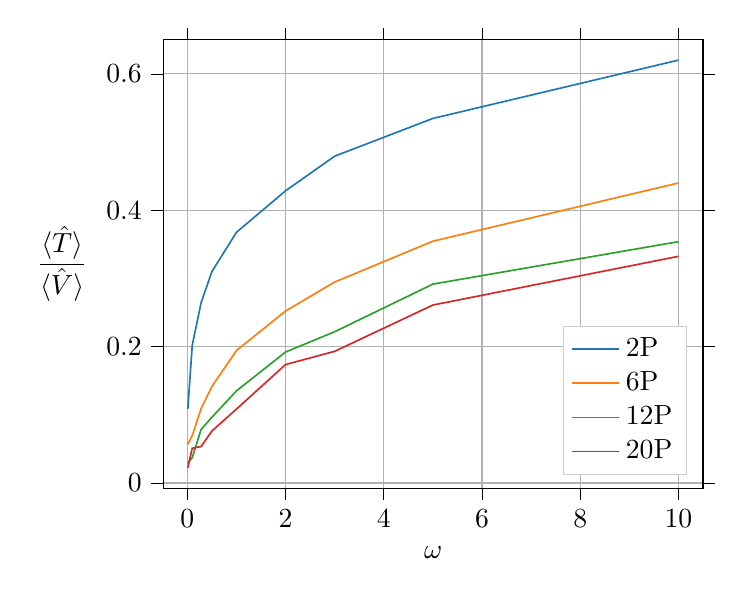
\begin{tikzpicture}

\definecolor{color0}{rgb}{0.12156862745098,0.466666666666667,0.705882352941177}
\definecolor{color1}{rgb}{1,0.498039215686275,0.0549019607843137}
\definecolor{color2}{rgb}{0.172549019607843,0.627450980392157,0.172549019607843}
\definecolor{color3}{rgb}{0.83921568627451,0.152941176470588,0.156862745098039}

\begin{axis}[
legend cell align={left},
legend style={at={(0.97,0.03)}, anchor=south east, draw=white!80.0!black},
tick align=outside,
tick pos=both,
x grid style={white!69.01960784313725!black},
xlabel={\(\displaystyle \omega\)},
xmajorgrids,
xmin=-0.4895, xmax=10.4995,
xtick style={color=black},
y grid style={white!69.01960784313725!black},
ylabel style={rotate=-90.0},
ylabel={\(\displaystyle \frac{\langle\hat{T}\rangle}{\langle\hat{V}\rangle}\)},
ymajorgrids,
ymin=-0.00739548914049018, ymax=0.649881709767761,
ytick style={color=black}
]
\addplot [semithick, color0]
table {%
0.01 0.108705258506407
0.1 0.202009646302251
0.28 0.264296187683284
0.5 0.310018755861207
1 0.367553865652725
2 0.428427393293865
3 0.479188481675393
5 0.534512711346008
10 0.620005473453749
};
\addlegendentry{2P}
\addplot [semithick, color1]
table {%
0.01 0.0567119155354449
0.1 0.0697142186491403
0.28 0.109019214224262
0.5 0.141514485132422
1 0.194234043802478
2 0.252176075603084
3 0.294666494223597
5 0.354539716887567
10 0.439893538370546
};
\addlegendentry{6P}
\addplot [semithick, color2]
table {%
0.01 0.0288659793814433
0.1 0.0372200263504611
0.28 0.0784915858002702
0.5 0.096412072256494
1 0.135095692138839
2 0.192092791484218
3 0.221784714644907
5 0.291641379310345
10 0.353855680855225
};
\addlegendentry{12P}
\addplot [semithick, color3]
table {%
0.01 0.0224807471735212
0.1 0.0510365183964855
0.28 0.0535270823545204
0.5 0.0761996706229769
1 0.108428284656055
2 0.17366909653192
3 0.19307880632568
5 0.260942252768941
10 0.332349732889548
};
\addlegendentry{20P}
\end{axis}

\end{tikzpicture}}}\\
	\subfloat[RBM+PJ]{{% This file was created by tikzplotlib v0.8.1.
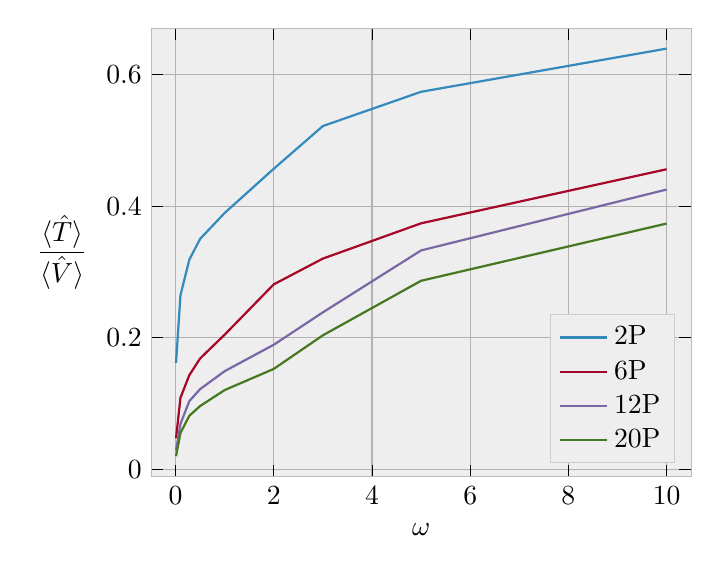
\begin{tikzpicture}

\definecolor{color0}{rgb}{0.203921568627451,0.541176470588235,0.741176470588235}
\definecolor{color1}{rgb}{0.650980392156863,0.0235294117647059,0.156862745098039}
\definecolor{color2}{rgb}{0.47843137254902,0.407843137254902,0.650980392156863}
\definecolor{color3}{rgb}{0.274509803921569,0.470588235294118,0.129411764705882}

\begin{axis}[
axis background/.style={fill=white!93.33333333333333!black},
axis line style={white!73.72549019607844!black},
legend cell align={left},
legend style={at={(0.97,0.03)}, anchor=south east, draw=white!80.0!black, fill=white!93.33333333333333!black},
tick pos=both,
x grid style={white!69.80392156862744!black},
xlabel={\(\displaystyle \omega\)},
xmajorgrids,
xmin=-0.4895, xmax=10.4995,
xtick style={color=black},
y grid style={white!69.80392156862744!black},
ylabel style={rotate=-90.0},
ylabel={\(\displaystyle \frac{\langle\hat{T}\rangle}{\langle\hat{V}\rangle}\)},
ymajorgrids,
ymin=-0.011155128448522, ymax=0.670716886119897,
ytick style={color=black}
]
\addplot [thick, color0]
table {%
0.01 0.161598746081505
0.1 0.264466364626943
0.28 0.318533815178111
0.5 0.350256285086649
1 0.389730328777244
2 0.456965583072599
3 0.52190696776684
5 0.574018126888218
10 0.639722703639515
};
\addlegendentry{2P}
\addplot [thick, color1]
table {%
0.01 0.0468986384266263
0.1 0.108489101409675
0.28 0.142927927927928
0.5 0.168400011874487
1 0.204595643091614
2 0.281150742944763
3 0.320306803143652
5 0.373984932084395
10 0.456212770963223
};
\addlegendentry{6P}
\addplot [thick, color2]
table {%
0.01 0.0287417763157895
0.1 0.0689267491135519
0.28 0.103510351035104
0.5 0.121754035137837
1 0.149081447331657
2 0.189290836653386
3 0.238556500646571
5 0.332749562171629
10 0.425379527774922
};
\addlegendentry{12P}
\addplot [thick, color3]
table {%
0.01 0.0198390540318607
0.1 0.0550696242390316
0.28 0.0812272164373049
0.5 0.0960548685344326
1 0.120346512979882
2 0.152555093728466
3 0.20363356015151
5 0.286590458917023
10 0.373618884667807
};
\addlegendentry{20P}
\end{axis}

\end{tikzpicture}}}
	\subfloat[VMC]{{% This file was created by tikzplotlib v0.8.1.
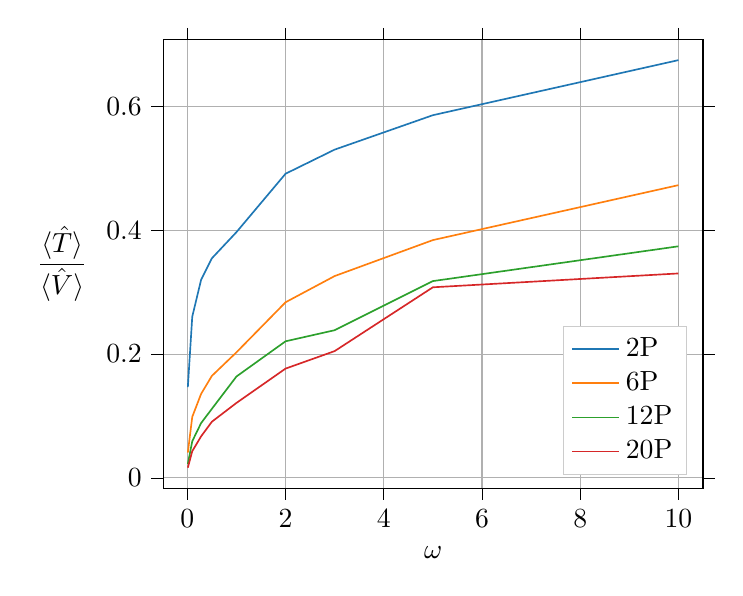
\begin{tikzpicture}

\definecolor{color0}{rgb}{0.12156862745098,0.466666666666667,0.705882352941177}
\definecolor{color1}{rgb}{1,0.498039215686275,0.0549019607843137}
\definecolor{color2}{rgb}{0.172549019607843,0.627450980392157,0.172549019607843}
\definecolor{color3}{rgb}{0.83921568627451,0.152941176470588,0.156862745098039}

\begin{axis}[
legend cell align={left},
legend style={at={(0.97,0.03)}, anchor=south east, draw=white!80.0!black},
tick align=outside,
tick pos=both,
x grid style={white!69.01960784313725!black},
xlabel={\(\displaystyle \omega\)},
xmajorgrids,
xmin=-0.4895, xmax=10.4995,
xtick style={color=black},
y grid style={white!69.01960784313725!black},
ylabel style={rotate=-90.0},
ylabel={\(\displaystyle \frac{\langle\hat{T}\rangle}{\langle\hat{V}\rangle}\)},
ymajorgrids,
ymin=-0.0164668337421715, ymax=0.707728537231861,
ytick style={color=black}
]
\addplot [semithick, color0]
table {%
0.01 0.146594427244582
0.1 0.260418749464423
0.28 0.319901846829394
0.5 0.354717597127
1 0.396972519795063
2 0.491318502441671
3 0.53027950310559
5 0.585870116692034
10 0.67481056582395
};
\addlegendentry{2P}
\addplot [semithick, color1]
table {%
0.01 0.0407722122838402
0.1 0.0985104942450914
0.28 0.135666711367395
0.5 0.164801025691602
1 0.202835527491511
2 0.28369079862382
3 0.326016767506851
5 0.384115256741781
10 0.472868887927304
};
\addlegendentry{6P}
\addplot [semithick, color2]
table {%
0.01 0.0225470925470925
0.1 0.0591952540624194
0.28 0.0885030700825746
0.5 0.111576919808515
1 0.163770657314416
2 0.220633968028807
3 0.238556500646571
5 0.317885405699147
10 0.37406475534662
};
\addlegendentry{12P}
\addplot [semithick, color3]
table {%
0.01 0.0164511376657391
0.1 0.0430938843433643
0.28 0.067074638154502
0.5 0.0907330085826954
1 0.121087634122869
2 0.176534004132603
3 0.20481414099371
5 0.307872099467483
10 0.330233868695407
};
\addlegendentry{20P}
\end{axis}

\end{tikzpicture}}}
	\caption{The kinetic-potential energy ratio $\langle\hat{T}\rangle/\langle\hat{V}\rangle$ plotted as a function of the oscillator frequency for two-dimensional circular quantum dots. The frequencies $\omega=0.01, 0.1, 0.28, 0.5, 1.0, 2.0, 3.0, 5.0, 10.0$ were run. For abbreviations see the text.}
	\label{fig:energysplitVMC2D}
\end{figure}
\fi

\subsection{Energy distribution} \label{sec:energydistributions}
If we now recall the general Hamiltonian presented in chapter \ref{chp:manybody}, the total energy is just the sum of the kinetic, potential, and interaction energy. As our methods attempt to solve the Schrödinger equation directly, it is trivial to find the distribution between the various energy sources, which in general is interesting when we want to find the most important contributor to the energy. Additionally, we can use those results to verify the virial theorem presented in section \ref{sec:virial}, and it is also interesting to see if the different methods give different energy distributions. In figure \eqref{fig:energydistribution}, we plot the ratio between the kinetic and potential energy as a function of oscillator frequency for two-dimensional quantum dots with up to $N=20$ electrons for all our methods. The plots are based on the numbers in the tables (\ref{tab:splitfrequencyQDVMC}-\ref{tab:splitfrequencyQDRBMPJ}) in appendix \ref{chp:totalresults}. 

% This file was created by tikzplotlib v0.8.1.
\begin{figure}
\begin{tikzpicture}

\begin{axis}[
legend cell align={left},
legend style={at={(1.7,1.15)}, anchor=south east, draw=white!80.0!black},
legend columns = 4,
title={RBM},
title style={yshift=-1.5ex},
%tick align=outside,
tick pos=both,
x grid style={white!69.01960784313725!black},
%xlabel={\(\displaystyle \omega\)},
width=8cm,
height=5cm,
xmajorgrids,
xmin=-0.4895, xmax=10.4995,
xtick style={color=black},
y grid style={white!69.01960784313725!black},
ylabel style={rotate=-90.0},
ylabel={\(\displaystyle \frac{\langle\hat{T}\rangle}{\langle\hat{V}\rangle}\)},
ymajorgrids,
ymin=-0.03, ymax=0.7,
ytick style={color=black}
]
\addplot [thick, color0]
table {%
	0.01 0.14292980671414
	0.1 0.206000508517671
	0.28 0.236346842166032
	0.5 0.277065579844387
	1 0.345784185233727
	2 0.41399969664796
	3 0.461449773987519
	5 0.512681528738802
	10 0.616027732463295
};
\addlegendentry{$N=2$}
\addplot [thick, color1]
table {%
	0.01 0.0489614243323442
	0.1 0.0953652097389264
	0.28 0.123020257826888
	0.5 0.151552210724365
	1 0.195728715728716
	2 0.296060131091479
	3 0.363623577547628
	5 0.440925380415408
	10 0.491388484677367
};
\addlegendentry{$N=6$}
\addplot [thick, color2]
table {%
	0.01 0.0279279279279279
	0.1 0.0663141106354403
	0.28 0.0927190456602221
	0.5 0.113307273027584
	1 0.152620094780267
	2 0.21978952717725
	3 0.263891885843983
	5 0.321107495449782
	10 0.357318784099766
};
\addlegendentry{$N=12$}
\addplot [thick, color3]
table {%
	0.01 0.0202855736090596
	0.1 0.0558188176084186
	0.28 0.0748673013733255
	0.5 0.092181964299863
	1 0.120447174205168
	2 0.191577362501107
	3 0.2257693437
	5 0.263982205508037
	10 0.278872126802915
};
\addlegendentry{$N=20$}
\end{axis}

\begin{axis}[
xshift=7.7cm,
legend cell align={left},
legend style={at={(0.97,0.03)}, anchor=south east, draw=white!80.0!black},
%tick align=outside,
title={RBM+SJ},
title style={yshift=-1.5ex},
tick pos=both,
x grid style={white!69.01960784313725!black},
%xlabel={\(\displaystyle \omega\)},
xmajorgrids,
width=8cm,
height=5cm,
xmin=-0.4895, xmax=10.4995,
xtick style={color=black},
y grid style={white!69.01960784313725!black},
%ylabel style={rotate=-90.0},
%ylabel={\(\displaystyle \frac{\langle\hat{T}\rangle}{\langle\hat{V}\rangle}\)},
ymajorgrids,
ymin=-0.03, ymax=0.7,
ytick style={color=black}
]
\addplot [thick, color0]
table {%
	0.01 0.108705258506407
	0.1 0.202009646302251
	0.28 0.264296187683284
	0.5 0.310018755861207
	1 0.367553865652725
	2 0.428427393293865
	3 0.479188481675393
	5 0.534512711346008
	10 0.620005473453749
};
%\addlegendentry{2P}
\addplot [thick, color1]
table {%
	0.01 0.0567119155354449
	0.1 0.0697142186491403
	0.28 0.109019214224262
	0.5 0.141514485132422
	1 0.194234043802478
	2 0.252176075603084
	3 0.294666494223597
	5 0.354539716887567
	10 0.439893538370546
};
%\addlegendentry{6P}
\addplot [thick, color2]
table {%
	0.01 0.0288659793814433
	0.1 0.0372200263504611
	0.28 0.0784915858002702
	0.5 0.096412072256494
	1 0.135095692138839
	2 0.192092791484218
	3 0.221784714644907
	5 0.291641379310345
	10 0.353855680855225
};
%\addlegendentry{12P}
\addplot [thick, color3]
table {%
	0.01 0.0224807471735212
	0.1 0.0510365183964855
	0.28 0.0535270823545204
	0.5 0.0761996706229769
	1 0.108428284656055
	2 0.17366909653192
	3 0.19307880632568
	5 0.260942252768941
	10 0.332349732889548
};
%\addlegendentry{20P}
\end{axis}

\end{tikzpicture}

\begin{tikzpicture}

\begin{axis}[
legend cell align={left},
legend style={at={(0.97,1.03)}, anchor=south east, draw=white!80.0!black},
%tick align=outside,
title={RBM+PJ},
title style={yshift=-1.5ex},
tick pos=both,
x grid style={white!69.01960784313725!black},
xlabel={\(\displaystyle \omega\)},
width=8cm,
height=5cm,
xmajorgrids,
xmin=-0.4895, xmax=10.4995,
xtick style={color=black},
y grid style={white!69.01960784313725!black},
ylabel style={rotate=-90.0},
ylabel={\(\displaystyle \frac{\langle\hat{T}\rangle}{\langle\hat{V}\rangle}\)},
ymajorgrids,
ymin=-0.03, ymax=0.75,
ytick style={color=black}
]
\addplot [thick, color0]
table {%
	0.01 0.161598746081505
	0.1 0.264466364626943
	0.28 0.318533815178111
	0.5 0.350256285086649
	1 0.389730328777244
	2 0.456965583072599
	3 0.52190696776684
	5 0.574018126888218
	10 0.639722703639515
};
%\addlegendentry{2P}
\addplot [thick, color1]
table {%
	0.01 0.0468986384266263
	0.1 0.108489101409675
	0.28 0.142927927927928
	0.5 0.168400011874487
	1 0.204595643091614
	2 0.281150742944763
	3 0.320306803143652
	5 0.373984932084395
	10 0.456212770963223
};
%\addlegendentry{6P}
\addplot [thick, color2]
table {%
	0.01 0.0287417763157895
	0.1 0.0689267491135519
	0.28 0.103510351035104
	0.5 0.121754035137837
	1 0.149081447331657
	2 0.189290836653386
	3 0.238556500646571
	5 0.332749562171629
	10 0.425379527774922
};
%\addlegendentry{12P}
\addplot [thick, color3]
table {%
	0.01 0.0198390540318607
	0.1 0.0550696242390316
	0.28 0.0812272164373049
	0.5 0.0960548685344326
	1 0.120346512979882
	2 0.152555093728466
	3 0.20363356015151
	5 0.286590458917023
	10 0.373618884667807
};
%\addlegendentry{20P}
\node[] at (axis cs: 5,-.25) {RBM+PJ};
\end{axis}

\begin{axis}[
xshift=7.7cm,
legend cell align={left},
legend style={at={(0.97,0.03)}, anchor=south east, draw=white!80.0!black},
%tick align=outside,
title={VMC},
title style={yshift=-1.5ex},
tick pos=both,
x grid style={white!69.01960784313725!black},
xlabel={\(\displaystyle \omega\)},
xmajorgrids,
width=8cm,
height=5cm,
xmin=-0.4895, xmax=10.4995,
xtick style={color=black},
y grid style={white!69.01960784313725!black},
%ylabel style={rotate=-90.0},
%ylabel={\(\displaystyle \frac{\langle\hat{T}\rangle}{\langle\hat{V}\rangle}\)},
ymajorgrids,
ymin=-0.03, ymax=0.75,
ytick style={color=black}
]
\addplot [thick, color0]
table {%
	0.01 0.146594427244582
	0.1 0.260418749464423
	0.28 0.319901846829394
	0.5 0.354717597127
	1 0.396972519795063
	2 0.491318502441671
	3 0.53027950310559
	5 0.585870116692034
	10 0.67481056582395
};

\addplot [thick, color1]
table {%
	0.01 0.0407722122838402
	0.1 0.0985104942450914
	0.28 0.135666711367395
	0.5 0.164801025691602
	1 0.202835527491511
	2 0.28369079862382
	3 0.326016767506851
	5 0.384115256741781
	10 0.472868887927304
};

\addplot [thick, color2]
table {%
	0.01 0.0225470925470925
	0.1 0.0591952540624194
	0.28 0.0885030700825746
	0.5 0.111576919808515
	1 0.163770657314416
	2 0.220633968028807
	3 0.238556500646571
	5 0.317885405699147
	10 0.37406475534662
};

\addplot [thick, color3]
table {%
	0.01 0.0164511376657391
	0.1 0.0430938843433643
	0.28 0.067074638154502
	0.5 0.0907330085826954
	1 0.121087634122869
	2 0.176534004132603
	3 0.20481414099371
	5 0.307872099467483
	10 0.330233868695407
};
\end{axis}

\end{tikzpicture}
\caption{The kinetic-potential energy ratio $\langle\hat{T}\rangle/\langle\hat{V}\rangle$ plotted as a function of the oscillator frequency for two-dimensional circular quantum dots with $N=2$, 6, 12 and 20 electrons. The frequencies $\omega=0.01,$ 0.1, 0.28, 0.5, 1.0, 2.0, 3.0, 5.0, 10.0 were run, see appendix \ref{chp:totalresults} for exact energies. For abbreviations see the text.}
\label{fig:energydistribution}
\end{figure}

Firstly, the graphs are very similar for all the methods, which means that they all give the same distribution between kinetic and potential energy, although they do not provide the same energy. This is an interesting observation and means that the obtained kinetic and potential energy are both different for the various methods when the total energy is different. Physically, this indicates that the electron configurations are fundamentally different for the different methods, which is the only factor that can cause a change in potential energy. This is already observed in the one-body density plots. Further, we see a significant trend where the ratio drops as the frequency is decreased, implying that the potential energy dominates the kinetic energy at low frequencies, which is a known phenomenon already mentioned several times throughout this thesis. For all the methods, the ratio is also lower for larger dots, which is a result of gradually more interaction energy as the number of particles increases.

\begin{table}
	\caption{This table shows how the total energy ($\langle\hat{H}\rangle$) is distributed between kinetic energy ($\langle\hat{T}\rangle$), external potential energy ($\langle\hat{V}_{\text{ext}}\rangle$) and interaction energy ($\langle\hat{V}_{\text{int}}\rangle$) for two-dimensional quantum dots with $N=12$ electrons and at a wide range of frequencies $\omega$. The energy is given in units of $\hbar$, and the numbers in parenthesis are the statistical uncertainties in the last digit. For abbreviations see the text.}
	\label{tab:splitfrequencyQD20P}
	\begin{tabularx}{\textwidth}{R{0.5cm}rrcR{2.3cm}R{2.3cm}R{2.3cm}R{2.3cm}R{0.3cm}} \hline\hline
		&\makecell{\\ \phantom{$N$}} & $\omega$ && \multicolumn{1}{c}{$\langle \hat{H}\rangle$} & \multicolumn{1}{c}{$\langle \hat{T}\rangle$} & \multicolumn{1}{c}{$\langle \hat{V}_{\text{ext}} \rangle$} & \multicolumn{1}{c}{$\langle \hat{V}_{\text{int}} \rangle$} \\ \hline \\
		&RBM & 0.01 && 6.217(2) & 0.1236(4) & 2.244(2) & 3.849(2) \\
		&& 2.0 && 269.086(8) & 43.262(8) & 95.17(2) & 130.65(1) \\
		&& 10.0 && 961.03(4) & 260.2(1) & 364.8(1) & 336.06(7) \\
		\hline \\
		
		&RBM+SJ & 0.01 && 6.239(2) & 0.1372(6) & 2.184(2) & 3.919(3) \\
		&& 2.0 && 265.66(9) & 39.31(8) & 95.78(1) & 130.57(2) \\
		&& 10.0 && 952.71(2) & 237.65(4) & 392.06(7) & 323.00(3) \\
		\hline \\
		
		&RBM+PJ & 0.01 && 6.210(1) & 0.1208(5) & 2.189(2) & 3.900(2) \\
		&& 2.0 && 262.598(1) & 34.758(6) & 108.546(9) & 119.293(7) \\
		&& 10.0 && 947.33(2) & 257.67(5) & 348.35(6) & 341.31(3) \\ 
		\hline \\
		
		&VMC & 0.01 && 6.2097(8) & 0.1005(4) & 2.270(3) & 3.839(3) \\
		&& 2.0 && 262.5339(9) & 38.402(3) & 95.681(7) & 128.451(5) \\
		&& 10.0 && 945.596(8) & 231.56(4) & 389.26(7) & 324.77(3) \\
		\hline\hline
	\end{tabularx}
\end{table}

If we further recall the virial theorem presented in section \ref{sec:virial}, it states that the kinetic energy is related to the potential energies in a certain way. If we assume that the interaction potential goes as $V_{\text{int}}\propto r^{-1}$, we can write the virial theorem as
\begin{empheq}[box={\mybluebox[5pt]}]{equation}
2\langle \hat{T} \rangle=2\langle \hat{V}_{\text{ext}} \rangle-\langle \hat{V}_{\text{int}} \rangle,
\label{eq:modifiedvirial}
\end{empheq}
according to equation \eqref{eq:simplevirial}. We could try to verify this formula from figure \eqref{fig:energydistribution}, but in order to do this accurately, we will list up the energy distributions for some selected systems. For a two-dimensional quantum dot with $N=20$ electrons the energy distribution is given in table \eqref{tab:splitfrequencyQD20P} for some selected frequencies. By doing the math, we see that the virial theorem is not satisfied for any of the methods or frequencies! For the lowest frequency, the theorem is far from being correct, but as the frequency increases the error decreases. To estimate the accuracy of the theorem, we introduce a ratio
\begin{equation}
R=\frac{2\langle\hat{T}\rangle}{2\langle\hat{V}_{\text{ext}}\rangle-\langle\hat{V}_{\text{int}}\rangle}
\end{equation}
which naturally is $R_{\text{exact}}=1$ if our version of the virial theorem is satisfied. To estimate the error, we calculate the absolute error $E_{\omega}=||R_{\omega}-1||$. Take, for example VMC, we get $E_{\omega=0.01}=0.713$, $E_{\omega=2}=0.221$ and $E_{\omega=10}=0.021$, which shows that equation \eqref{eq:modifiedvirial} gradually gets more accurate as the potential energy gets more important. To see why this is the case, we need to go back to the original virial theorem given in equation \eqref{eq:virialtheorem}. By inserting the interaction energy, we see that our modified virial theorem is inaccurate, and breaks down when the interaction energy dominates. However, it should be quite accurate when the interaction energy is not so important, which is consistent with our results. 

Another interesting thing is how the energy is distributed for the various methods. Most notably, we see that VMC and RBM+PJ provide different distributions between the different methods, albeit the total energy is more or less identical. Physically, this means that the RBM+PJ finds another configuration than VMC to minimize the energy, which is exciting as the former method is supposed to be more flexible than the latter. For more frequencies and system sizes, please look at appendix \ref{chp:totalresults}.

\begin{figure}
	\centering
	\captionsetup[subfigure]{labelformat=empty}
	\subfloat{\raisebox{1.5cm}{\rotatebox[origin=t]{90}{RBM}}}\hspace{0.1cm}
	\subfloat{{\includegraphics[width=5.1cm]{../plots/int1/onebody2/2D/2P/0.100000w/RBM_ADAM_MC1048576.png}}}\hspace{-0.cm}
	\subfloat{{\includegraphics[width=5.1cm]{../plots/int1/onebody2/2D/6P/0.100000w/RBM_ADAM_MC1048576.png}}}\hspace{-0.cm}
	\subfloat{{\includegraphics[width=5.1cm]{../plots/int1/onebody2/2D/12P/0.100000w/RBM_ADAM_MC1048576.png}}}\\ [-0.cm]
	
	\subfloat{\raisebox{1.5cm}{\rotatebox[origin=t]{90}{VMC}}}\hspace{0.1cm}
	\subfloat[$N=2$]{{\includegraphics[width=5.1cm]{../plots/int1/onebody2/2D/2P/0.100000w/VMC_ADAM_MC1048576.png}}}\hspace{-0.cm}
	\subfloat[$N=6$]{{\includegraphics[width=5.1cm]{../plots/int1/onebody2/2D/6P/0.100000w/VMC_ADAM_MC1048576.png}}}\hspace{-0.cm}
	\subfloat[$N=12$]{{\includegraphics[width=5.1cm]{../plots/int1/onebody2/2D/12P/0.100000w/VMC_ADAM_MC1048576.png}}}
	
	\caption{One-body density of two-dimensional circular quantum dots with frequency $\omega=0.1$ with $N=2$, 6 and 12 electrons, where the surface plot and the contour plot on the $xy$-plane illustrate the density and the graph on the $yz$-plane represents the cross-section through $x=0$. The surface plots are noise-reduced using a Savitzky-Golay filter, and for abbreviations see the text.}
	\label{fig:lowfreqRBM}
\end{figure}

\newpage
\subsection{Low frequency dots} \label{sec:lowfrequencies}
In section \ref{sec:onebodyresults}, we found the one-body density to be shape-invariant for high-frequency dot with $\omega\geq0.28$. However, when we further decreased the frequency down to $\omega=0.1$, the density profiles changed significantly, and we got other extrema and so on. This section aims to investigate the transitions between the various shapes with frequencies down to $\omega=0.01$. We start by looking at quantum dots with frequency $\omega=0.1$, and in figure \eqref{fig:lowfreqRBM} we compare the radial density profiles for $N=2$, 6 and 12 produced by RBM to the results produced by VMC. What we observe is that the density plots are completely different. While VMC provides a single peak with some bumps on the top, RBM gives several peaks for all the numbers of electrons. The numbers of peaks apparently is equal to the number of electrons, which indicates that the RBM finds the electrons to be localized at some fixed spots. The two methods model the correlations in completely different ways, and as the correlations become more important for low frequencies, it was expected that the results would also be different. However, the obtained ground state energies by the two methods are not so different for the same systems, indicating that the electron density plots are better at reveal differences between the methods than the energy itself. 

\begin{figure}
	\centering
	\captionsetup[subfigure]{labelformat=empty}
	\subfloat{\raisebox{1.5cm}{\rotatebox[origin=t]{90}{RBM+PJ}}}\hspace{0.1cm}
	\subfloat{{\includegraphics[width=5.1cm]{../plots/int1/onebody2/2D/2P/0.280000w/RBMPJ_ADAM_MC1048576.png}}}\hspace{-0.cm}
	\subfloat{{\includegraphics[width=5.1cm]{../plots/int1/onebody2/2D/2P/0.100000w/RBMPJ_ADAM_MC1048576.png}}}\hspace{-0.cm}
	\subfloat{{\includegraphics[width=5.1cm]{../plots/int1/onebody2/2D/2P/0.010000w/RBMPJ_ADAM_MC2pow28_smooth_blue_small.png}}}\\ [-0.cm]
	
	\subfloat{\raisebox{1.5cm}{\rotatebox[origin=t]{90}{VMC}}}\hspace{0.1cm}
	\subfloat[$\omega=0.28$]{{\includegraphics[width=5.1cm]{../plots/int1/onebody2/2D/2P/0.280000w/VMC_ADAM_MC1048576.png}}}\hspace{-0.cm}
	\subfloat[$\omega=0.1$]{{\includegraphics[width=5.1cm]{../plots/int1/onebody2/2D/2P/0.100000w/VMC_ADAM_MC1048576.png}}}\hspace{-0.cm}
	\subfloat[$\omega=0.01$]{{\includegraphics[width=5.1cm]{../plots/int1/onebody2/2D/2P/0.010000w/VMC_ADAM_MC2pow28_smooth_blue_small.png}}}
	
	\caption{One-body density of two-dimensional circular quantum dots with $N=2$ electrons and frequencies $\omega=0.28$, 0.1 and 0.01, where the surface plot and the contour plot on the $xy$-plane illustrate the density and the graph on the $yz$-plane represents the cross-section through $x=0$. The surface plots are noise-reduced using a Savitzky-Golay filter, and for abbreviations see the text.}
	\label{fig:lowfreq2P}
\end{figure}

Further, we fix the number of electrons to be $N=2$, and vary the frequency from $\omega=0.28$ down to $\omega=0.01$ with density profiles produced by VMC and RBM+PJ found in figure \eqref{fig:lowfreq2P}. Those methods were selected as they hitherto have shown the most promising results and we want to see if the RBM+PJ can reveal effects that the VMC is not able to capture. We see that the two methods obtain very similar density plots, where they agree that a ridge around the center of the dot should be more distinct as the frequency drops. If we go back to figure \eqref{fig:energydistribution}, we saw that the kinetic energy was negligible for the lowest energies, and the effect is, therefore, an indication of the Wigner localization effect discussed in section \ref{sec:wigner}. As in the classical limit, the two electrons will repel each other and seldom be located at the same place when their kinetic energy is low. RBM+PJ possibly provides a sharper ridge for $\omega=0.01$, which is closer to the DMC results found from \citet{hogberget_quantum_2013} and thus perhaps more correct. However, the energy provided by RBM+PJ and VMC are more or less identical (0.074107 and 0.074070 respectively), which means that the potential difference does not give effect to the energy.

\begin{figure}
	\centering
	\captionsetup[subfigure]{labelformat=empty}
	\subfloat{\raisebox{1.5cm}{\rotatebox[origin=t]{90}{RBM+PJ}}}\hspace{0.1cm}
	\subfloat{{\includegraphics[width=5.1cm]{../plots/int1/onebody2/2D/6P/0.280000w/RBMPJ_ADAM_MC1048576.png}}}\hspace{-0.cm}
	\subfloat{{\includegraphics[width=5.1cm]{../plots/int1/onebody2/2D/6P/0.100000w/RBMPJ_ADAM_MC1048576.png}}}\hspace{-0.cm}
	\subfloat{{\includegraphics[width=5.1cm]{../plots/int1/onebody2/2D/6P/0.010000w/RBMPJ_ADAM_MC1048576.png}}}\\ [-0.cm]
	
	\subfloat{\raisebox{1.5cm}{\rotatebox[origin=t]{90}{VMC}}}\hspace{0.1cm}
	\subfloat[$\omega=0.28$]{{\includegraphics[width=5.1cm]{../plots/int1/onebody2/2D/6P/0.280000w/VMC_ADAM_MC1048576.png}}}\hspace{-0.cm}
	\subfloat[$\omega=0.1$]{{\includegraphics[width=5.1cm]{../plots/int1/onebody2/2D/6P/0.100000w/VMC_ADAM_MC1048576.png}}}\hspace{-0.cm}
	\subfloat[$\omega=0.01$]{{\includegraphics[width=5.1cm]{../plots/int1/onebody2/2D/6P/0.010000w/VMC_ADAM_MC2pow28_smooth}}}
	
	\caption{One-body density of two-dimensional circular quantum dots with $N=6$ electrons and frequencies $\omega=0.28$, 0.1 and 0.01, where the surface plot and the contour plot on the $xy$-plane illustrate the density and the graph on the $yz$-plane represents the cross-section through $x=0$. The surface plots are noise-reduced using a Savitzky-Golay filter, and for abbreviations see the text.}
	\label{fig:lowfreq6P}
\end{figure}

We repeat the exercise for quantum dots with $N=6$ electrons, and obtain the plots in figure \eqref{fig:lowfreq6P}. When using VMC, we observe the same tendency as for the dots with $N=2$ electrons, where we get an additional peak in the density plot as the frequency decreases. However, for RBM+PJ, we do not get this peak in the center, but rather a significant density drop. This is contrary to the DMC one-body density plots obtained by \citet{hogberget_quantum_2013}, where it is a sharp peak in the center. The density plot for quantum dots is also known to approach the classical limit as the frequency is decreased \cite{ghosal_incipient_2007}, where the potential energy is minimized when we have one electron in the center and five electrons surrounding it. In other words, RBM+PJ appears to be wrong for this case. 

In order to give a more qualitative comparison of the various methods, we also present the radial one-body density profile of the quantum dots of frequency $\omega=0.01$ with $N=2$ and $N=6$ electrons, see figure \eqref{fig:lowfreq}. We see that all the methods agree for $N=2$, where RBM+PJ gives the most distinct peak, followed by VMC, RBM+SJ and RBM. For $N=6$, however, the various methods give completely different density profiles. As discussed for the spatial density profile, we believe that the VMC is the most correct because of the peak in the center. 

\begin{figure}
	\centering
	\captionsetup[subfigure]{labelformat=empty}
	\subfloat{{\includegraphics[width=\textwidth/2]{../plots/int1/onebody/2D/2P/0.010000w/ADAM_MC1048576.eps}}}
  	\subfloat{{\includegraphics[width=\textwidth/2]{../plots/int1/onebody/2D/6P/0.010000w/ADAM_MC10485762.eps}}}
	
	\caption{One-body density of two-dimensional quantum dots of frequency $\omega=0.01$ and $N=72$, 90. The ADAM optimizer was used, and after convergence the number of Monte-Carlo cycles was $M=2^{28}=268,435,456$. For abbreviations see the text.}
	\label{fig:lowfreq}
\end{figure}

\iffalse
\subsection{$S\neq0$}
When the number of particles in the quantum dot is among the magic numbers presented in equation \eqref{eq:HOclosedshell}, the ground state is guaranteed to be found at $L=S=0$. However, if we want to look at dots of other sizes, this is often not true, and we will, therefore, look at some cases with $S\neq 0$. We will still stick to $L=0$ and closed-shell systems.

Imagine a dot of four particles with $S=1$ (three have spin-up, and the last has spin-down). The ground state is obviously found when a spin up and a spin down particle is in the lowest energy state, and the remaining particles are in the first excited energy state. Since the lowest states and the first excited states with spin up are filled up, this is a closed shell system.

Again, our results will be benchmarked to DMC, with references Ref.\cite{pederiva_diffusion_2000} and Ref.\cite{ghosal_incipient_2007}. The former reference also presents Hartree-Fock results which we also will use. 

The results are listed in table \eqref{tab:sneq0}, where we use a restricted Boltzmann machine with Padé-Jastrow factor (RBM+PJ) and standard variational Monte-Carlo (VMC). 

We find both the RBM+PJ and VMC to reproduce the reference energy in all the cases. 

\begin{table}
	\caption{The ground state energy of two-dimensional circular quantum dots of frequency $\omega$ for a given spin configuration ($L$,$S$). The results were obtained by a restricted Boltzmann machine with Padé-Jastrow factor (RBM+PJ) and standard variational Monte-Carlo (VMC). For reference, the Hartree-Fock limit results from Ref.\cite{pederiva_diffusion_2000} (HF) and diffusion Monte-Carlo results from Refs.\cite{pederiva_diffusion_2000},\cite{ghosal_incipient_2007} (DMC) are listed. All energies are given in units of $\hbar$, and the numbers in parenthesis are the statistical uncertainties in the last digit.}
	\label{tab:sneq0}
	\begin{tabularx}{\textwidth}{rrXrrXR{2.3cm}R{2.3cm}R{2.3cm}R{2.3cm}} \hline\hline
		\makecell{\\ $N$ \\ \phantom{=}} & \makecell{$\omega$} & \phantom{R} & $L$ & $S$ & \phantom{R} & \multicolumn{1}{c}{RBM+PJ} & \multicolumn{1}{c}{VMC} & \multicolumn{1}{c}{\makecell{HF\\ (Ref.\cite{pederiva_diffusion_2000})}} & \multicolumn{1}{c}{\makecell{DMC\\ (Ref.\cite{pederiva_diffusion_2000})$^a$\\ (Ref.\cite{ghosal_incipient_2007})$^b$}} \\ \hline \\
		4 & 0.28 && 0 & 1 && 3.7475(2) & 3.7711(5) & 3.9033 & 3.7135(3)$^a$\\ \\
		8 & 0.28 && 0 & 1 && 12.828(3) & 12.849(1) & 13.1887 & 12.6903(7)$^a$ \\
		& 0.25 && 0 & 1 && 11.807(1) & 11.852(1) & - & 11.6697(1)$^b$ \\ \\
		9 & 0.28 && 0 & 3/2 && 15.886(4) & 15.812(4) & 16.1544 & 15.4784(7)$^a$\\
		&3.0 && 0 & 3/2 && 97.164(4) & 96.936(7) & - & 97.0095(3)$^b$\\ \\
		11 & 0.28 && 0 & 1/2 && 22.285(2) & 22.252(1) & 22.8733 & 22.0750(4)$^a$ \\ \hline\hline
	\end{tabularx}
\end{table}
\fi

\subsection{Large dots}
In order to test the code, we also decided to run for systems with $N>56$. This has no scientific significance, other than testing how far a VMC code can go. One thing is that the computations get extremely expensive as the number of particles increases, but we have also seen that the statistical error increases as the system size increases. This means that we cannot just crack up the wall clock time and wait when studying large systems; at some point, the standard error gets insufficiently large, and we need to increase the number of Monte Carlo cycles further. The learning rate also needs to be decreased as the system sizes increase, which requires more iterations.  We look at weakly interacting particles, so we will not get any relativistic effects even when adding many particles. In table \eqref{tab:largeQD}, the ground state energy of quantum dots with frequency $\omega=1.0$ and $N=72$, 90 electrons in two dimensions and $N=70$ particles in three dimensions is listed. We observe that the difference between VMC and RBM is quite significant, especially for $N=90$ electrons in two dimensions. We suspect that this simulation simply has not converged. 

\begin{table}
	\caption{Energy of large quantum dots with $N=72$ and 90, and $\omega=1.0$. All energies are given in units of $\hbar$, and the numbers in parenthesis are the statistical uncertainties in the last digit. For abbreviations see the text.}
	\label{tab:largeQD}
	\begin{tabularx}{\textwidth}{R{1.6cm}R{2cm}R{2cm}R{3cm}R{3cm}} \hline\hline
		& \makecell{\\ \phantom{$N$}} & $N$ & RBM & VMC \\ \hline \\
		& 2D & 72 & 1355.37(2) & 1340.520(7) \\
		&& 90 & 2194.12(9) & 1990.89(2) \\
		& 3D & 70 & 1129.40(2) & 1108.950(4) \\
		\hline \hline
	\end{tabularx}
\end{table}

In figure \eqref{fig:largedotsOB}, the radial one-body density profile is plotted for two-dimensional quantum dots with frequency $\omega=1.0$ and $N=72$, 90 electrons. Again, we observe the same peaks as we observed in section \ref{sec:onebodyresults}, and the number of peaks substantiates that we get an additional peak every time we add a closed-shell. However, for $N=90$, the peaks are not as significant as before, most notably for the RBM, which is another evidence that the simulation has not converged.

\begin{figure}
	\centering
	\captionsetup[subfigure]{labelformat=empty}
	\subfloat[$N=72$]{\includegraphics[width=8cm]{../plots/int1/onebody/2D/72P/1.000000w/ADAM_MC1048576.png}}\hspace{-0.5cm}
	\subfloat[$N=90$]{\includegraphics[width=8cm]{../plots/int1/onebody/2D/90P/1.000000w/ADAM_MC1048576.png}}\\
	\caption{Radial one-body density profile of large quantum dots with $N=72$ and 90, and frequency $\omega=1.0$ produced with RBM and VMC. The methods were detailed in the introductory words to this chapter, and for abbreviations see the text.}
	\label{fig:largedotsOB}
\end{figure}

\iffalse
\begin{figure}[H]
	\centering
	\subfloat[RBM]{\includegraphics[scale=0.4]{../plots/int1/twobody/2D/72P/1.000000w/RBM_ADAM_MC2pow28.png}}
	\subfloat[VMC]{\includegraphics[scale=0.4]{../plots/int1/twobody/2D/72P/1.000000w/RBM_ADAM_MC2pow28.png}}
	\caption{One-body density of large two-dimensional circular quantum dots with frequency $\omega=1.0$ containing 72 particles.}
	\label{fig:largedotsTB}
\end{figure}
\fi

\iffalse
\section{Double quantum dots}
Double quantum dots are systems that are very interesting when it comes to testing the Boltzmann machines. Even though we know the wave functions for the non-interacting case, they are expansions that are computationally expensive to work with.

\subsection{Ground state energy}
For the interacting case, we will use Alocias Mariadason's VMC calculations with and without a Hartree-Fock basis as a reference. Additionally, Høgberget provides a DMC energy for the case with two particles and $\omega=1.0$. All the results are given in table \eqref{tab:doubleQD}.
\begin{table}
	\caption{Double quantum dots. F is the number of functions used in the expansion.}
	\label{tab:doubleQD}
	\begin{tabularx}{\textwidth}{rrXR{2.3cm}R{2.3cm}R{2.3cm}R{2.3cm}R{2.3cm}} \hline\hline
		\makecell{\\ $N$ \\ \phantom{=}} & $\omega$ & \phantom{R} & \multicolumn{1}{c}{VMC (F=1)} & \multicolumn{1}{c}{RBM+PJ} & \multicolumn{1}{c}{\makecell{VMC (F$>$1)\\ (Ref.\cite{mariadason_quantum_2018})}} & \multicolumn{1}{c}{\makecell{VMC+HF\\ (Ref.\cite{mariadason_quantum_2018})}} & \multicolumn{1}{c}{\makecell{DMC\\ (Ref.\cite{hogberget_quantum_2013})}} \\ \hline \\
		2 & 0.1 && 0.41982(4) & 0.41939(3)\\
		& 0.28 && 0.9365(1) & 0.92618(4) \\
		& 0.5 && 1.4847(2) & 1.44004(4) \\
		& 1.0 && 2.6331(5) & 2.38342(3) & 2.42238(4) & 2.36618(4) & 2.3496(1) \\ \hline \\
		
		4 & 0.1 \\
		& 0.28 \\
		& 0.5 \\
		& 1.0 && - & - & 7.95247(4) & 7.90232(4) & - \\ \hline \\
		
		6 & 0.1 \\
		& 0.28 \\
		& 0.5 \\
		& 1.0 && - & - & 16.61419(4) & 16.55609(4) \\ \hline \\
		
		8 & 0.1 \\
		& 0.28 \\
		& 0.5 \\
		& 1.0 && - & - & \\ \hline \hline
	\end{tabularx}
\end{table}
What we observe, is that the Boltzmann machine with a Padé-Jastrow factor outperforms a Hermite expansion of 10 functions, which is surprising. The reason might be that the Boltzmann machine consists of a sum over all hidden nodes, which makes it behave similar to an expansion. However, the Boltzmann machine was then again beat by the Hermite expansion with a Hartree-Fock basis. 
\fi

\newpage
\section{Atoms}\label{sec:atomsresults}
The next systems we will address are the real atomic systems, which have been investigated by physicists since the childhood of quantum mechanics. This section is added to show the flexibility of the implemented code, which can easily be expanded to new systems. We use the simple hydrogen-like orbitals in our calculations, detailed in section \ref{sec:atomic}. In table \eqref{tab:atomswinteraction} we present the ground state energy of the four smallest closed-shell atoms Helium, Beryllium, Neon, and Magnesium, including an overview of how the energy is distributed and the ratio between kinetic and potential energy. We also compare the obtained results to experimental values. What we see is that the total energy is similar but slightly higher than our reference, which is as expected as we use a simple basis.

\begin{table}[H]
	\caption{Ground state energy of neutral atoms with atomic number $Z$ produced by VMC. We present the total energy ($\langle\hat{H}\rangle$), the external potential energy ($\langle\hat{V}_{\text{ext}}\rangle$), the interaction energy ($\langle\hat{V}_{\text{int}}\rangle$), the kinetic-potential energy ratio ($\langle\hat{T}\rangle/\langle\hat{V}\rangle$) and experimental values (Expr.). The latter were taken from \citet{degroote_faddeev_2013}, table 4.4. The energy is given in atomic units, and the numbers in parenthesis is the statistical error. For abbreviations see the text.}
	\label{tab:atomswinteraction}
	\begin{tabularx}{\textwidth}{lrrR{2cm}R{1.9cm}|R{1.7cm}R{1.7cm}R{1.7cm}R{1.7cm}} \hline\hline
		Atom & $Z$ & \makecell{\\ \phantom{=} \\ \phantom{=}} & 
		\multicolumn{1}{c}{\makecell{Expr.\\ (Ref.\cite{degroote_faddeev_2013})}} & \multicolumn{1}{c}{$\langle\hat{H}\rangle$} & \multicolumn{1}{c}{$\langle\hat{T}\rangle$} & \multicolumn{1}{c}{$\langle\hat{V}_{\text{ext}}\rangle$} & \multicolumn{1}{c}{$\langle\hat{V}_{\text{int}}\rangle$} & \multicolumn{1}{c}{$\langle\hat{T}\rangle/\langle\hat{V}\rangle $} \\ \hline \\
		
		He & 2 && -2.9037 & -2.8719(3) & 2.813(3) & -6.696(4) & 1.010(7) & -0.495 \\
		Be & 4 && -14.6674 & -14.4992(5) & 15.465(6) & -34.987(7) & 5.023(1) & -0.516 \\
		Ne & 10 && -128.9383 & -128.09(1) & 133.4(2) & -318.4(2) & 56.94(5) & -0.510 \\ 
		Mg & 12 && -200.054 & -196.81(4) & 251.9(2) & -557.0(2) & 108.23(6) & -0.379 \\ \hline\hline
	\end{tabularx}
\end{table}

If we once again recall the virial theorem first introduced in section \ref{sec:virial}, it reads
\begin{empheq}[box={\mybluebox[5pt]}]{equation}
2\langle\hat{T}\rangle = -(\langle\hat{V}_{\text{ext}}\rangle + \langle\hat{V}_{\text{int}}\rangle)
\label{eq:virialratio}
\end{empheq}
for atoms and molecules under the assumption that $V_{\text{int}}\propto r^{-1}$. For quantum dots, we found this assumption to be inaccurate, and our modified virial theorem broke down for strongly interacting systems. To see if the same happens fro atoms, we again introduce the ratio between the kinetic and potential energy, $R=\langle\hat{T}\rangle/\langle\hat{V}\rangle$, which for this system should be $R=-0.5$ in order to fulfill equation \eqref{eq:virialratio}. In the last column of table \ref{tab:atomswinteraction}, this ratio is presented for the various atoms, and for Helium, Beryllium and Neon we see that the ratio actually is close to -0.5. However, for Magnesium, the value is off, which could either be a result of too strong attraction force from the nucleus or some errors in the calculations. We believe that it is the latter, as we get an accurate result with Neon, and perhaps the model has just not converged. 
\begin{figure}
	\centering
	\captionsetup[subfigure]{labelformat=empty}
	\subfloat[Helium]{\includegraphics[width=\textwidth/2]{../plots/int1/atoms/He/ADAM_MC2pow28.png}}
	\subfloat[Beryllium]{\includegraphics[width=\textwidth/2]{../plots/int1/atoms/Be/ADAM_MC2pow28.png}}\\
	\subfloat[Neon]{\includegraphics[width=\textwidth/2]{../plots/int1/atoms/Ne/ADAM_MC2pow28.png}}
	\subfloat[Magnesium]{\includegraphics[width=\textwidth/2]{../plots/int1/atoms/Mg/ADAM_MC2pow28.png}}
	\caption{Radial one-body density profiles, $\rho(r)$, as a function of the radial distance from the nucleus, multiplied with $r^2$ in order to reveal fluctuations. We look at the Helium atom (upper left), the Beryllium atom (upper right), the Neon atom (lower left) and the Magnesium atom (lower right). VMC was used, which is detailed in the text. The number of Monte Carlo cycles used was $M=2^{28}=268,435,456$ and the ADAM optimizer was used. Hartree atomic units were used, see appendix \ref{app:units}.}
	\label{fig:atomsonebody}
\end{figure}
Further, we look at the radial one-body density profiles, which are presented in figure \eqref{fig:atomsonebody} for our four atoms. To reveal details, they are multiplied with $r^2$ as for example \citet{hogberget_quantum_2013} has done before us. We observe that the densities mostly are similar to his DMC results, which again substantiates that our framework and electron density computations work as they should. However, for Magnesium, the density plot is slightly different, which probably is related to the potential bug discussed above. 


\chapter{Conclusion}

\section{Summary of Results}
The aim of this thesis project is twofold: to create a quantum computing library that is oriented towards physicists and to study the performance of the Variational Quantum Eigensolver (VQE) and the Adaptive, Problem Tailor (ADAPT) VQE to obtain some insights for the best practices in using these algorithms. 

We built Quanthon as a result, which contains the basic elements to be able to perform any quantum operation. The \texttt{Hamiltonian} class was made to allow the Hamiltonians to be entered in a low-level way by specifying the one- and two-body coefficients. Other functionalities include the \texttt{VQE} and \texttt{ADAPT-VQE} classes which are the main focus of this project, as well as different modules that can assist the quantum simulations, including the mappers to convert fermionic Hamiltonians or matrix Hamiltonians to qubit Hamiltonians, the staircase and inverted staircase algorithms for converting exponentials of Pauli strings to quantum circuits, and the expectation value estimator which simulates the measurements of the quantum circuits and computes the expectation values of the Hamiltonians. 

With the library built, we then proceeded to study the performance of the VQE with hardware efficient ansatzes and ADAPT-VQE with two different minimal complete pools, the $ V $ and the $ G $ pool defined in Subsection~\ref{sub:qubit_adapt_vqe}, through both exact energy and ideal simulations of the multiple models. With the exact energy simulation, we observed that the hardware efficient ansatz in many cases does not converge to the ground state. When it does, the relative error is usually of order $ 10^{-2} $. The ADAPT-VQE with minimal pools, however, can indeed converge to the ground state with relative error lower than $ 10^{-6} $ given enough ADAPT iterations. The number of iterations it takes for the qubit-ADAPT-VQE to converge scales roughly linearly with the number of qubits in the model and the choice of the optimiser is independent of the number of iterations required. The best optimiser for the VQE was found to be the Powell method, and the best optimiser for the qubit-ADAPT-VQE was the BFGS method. 

In the presence of shot noise, the convergence of the qubit-ADAPT-VQE slows down but is still more stable and consistently outperforms the hardware efficient ansatz. We compared the error with the expected error from the number of shots to see if the algorithms have converged. The best optimiser, in this case, is the COBYLA method for the qubit-ADAPT-VQE and the Powell method for the VQE. We noticed that the ADAPT-VQE rarely exits due to the gradient being below the tolerance level, which is likely due to the noise.

No significant differences were observed in the performances of the $ V $ and $ G $ pool, except in the case of large pairing strength the $ G $ pool converges much faster than the $ V $ pool.

Additionally, we found that the gradient for all the operators in the minimal complete pool can be $ 0 $ for many Hamiltonians if the state is initialised in the $ \ket{0} $ state. This causes the ADAPT-VQE to exit immediately without any iterations. Initialising randomly avoids this problem but causes slow convergence. First, we used the maximally superposed state as an initial state. Later, we found that by initialising the ADAPT-VQE with the optimised state from hardware efficient ansatz boosts performances by reducing the number of iterations it takes for the ADAPT-VQE to converge. 

\section{Future Work}

We will group future work into two categories: improvements to the Quanthon library and improvements to the VQE and ADAPT-VQE algorithms.

\subsection{Improvements to Quanthon}
Many functionalities can be added to the Quanthon Library, such as adding more predefined gates or other popular algorithms. We could also explore other mappers, such as the Bravyi-Kitaev transformation~\cite{Seeley2012}. To increase the speed of simulations we could parallelise the measurements and add an option to group commuting terms of the Hamiltonian to be measured simultaneously. Integration with quantum hardware could also be extremely useful to allow the library to run on real quantum devices. More ansatzes could be implemented to allow for flexibility and performance comparison, specifically the unitary coupled cluster ansatz~\cite{Romero2019} and the fermionic-ADAPT ansatz~\cite{grimsley2019}. This would allow for a more comprehensive comparison of the ansatz. Another interesting direction would be to implement noise models to allow for noisy simulations.
\subsection{Improvements to Simulation Results}
The ideal simulation takes a long time to run, therefore the maximum number of iterations was all set to below $ 30 $, the performance of the ADAPT-VQE could potentially be improved by simply allowing the algorithm to run for more iterations. The $ 0 $ gradient problem is also concerning as the initial state could cause the algorithm to exit prematurely. More research is needed to find out under which circumstance would the gradient vanish and come up with either a different operator selection criteria for choosing an operator to be appended to the ansatz, or a systematic way to select the initial state to avoid the difficulty in convergence.



\clearpage
\phantomsection
\addcontentsline{toc}{chapter}{Bibliography}
\bibliographystyle{IEEEtran}
\bibliography{../bibtex/bibtex.bib}

\end{document}
